\documentclass[a4paper, 12pt]{report}
\usepackage{tikz}
\usetikzlibrary{shapes,arrows,positioning}
\usepackage{cmap}
\usepackage{tabularx}
\usepackage{amssymb}
\usepackage{amsmath}
\usepackage{graphicx}
\usepackage{amsthm}
\usepackage{amsmath}
\usepackage{amssymb}
\usepackage{upgreek}
\usepackage{setspace}
\usepackage{empheq}
\usepackage{mathtools}
\usepackage{listings}
\usepackage{pdflscape}
\usepackage{tikz}
\setcounter{secnumdepth}{5}
\setcounter{tocdepth}{5}
\numberwithin{equation}{section}
\renewcommand{\theequation}{\arabic{equation}}
\usepackage[T2A]{fontenc}
\usepackage[utf8]{inputenc}
\usepackage[normalem]{ulem}
\usepackage{mathtext} % русские буквы в формулах
\usepackage[left=2cm,right=2cm, top=2cm,bottom=2cm,bindingoffset=0cm]{geometry}
\usepackage[english,russian]{babel}
\usepackage[unicode]{hyperref}

\renewcommand{\leq}{\leqslant}
\renewcommand{\geq}{\geqslant}

\renewcommand{\alpha}{\upalpha}
\renewcommand{\beta}{\upbeta}
\renewcommand{\gamma}{\upgamma}
\renewcommand{\delta}{\updelta}
\renewcommand{\varphi}{\upvarphi}
\renewcommand{\phi}{\upvarphi}
\renewcommand{\tau}{\uptau}
\renewcommand{\theta}{\uptheta}
\renewcommand{\eta}{\upeta}
\renewcommand{\lambda}{\uplambda}
\renewcommand{\sigma}{\upsigma}
\renewcommand{\psi}{\uppsi}
\renewcommand{\mu}{\upmu}
\renewcommand{\omega}{\upomega}
\renewcommand{\xi}{\upxi}
\renewcommand{\epsilon}{\upvarepsilon}
\renewcommand{\rho}{\uprho}
\renewcommand{\varepsilon}{\upvarepsilon}

\newcommand{\pderiv}[2]{\dfrac{\partial #1}{\partial #2}}
\newcommand{\pderivtwo}[3]{\dfrac{\partial^2 #1}{\ifstrequal{#2}{#3}{\partial #2^2}{\partial #2 \partial #3}}}
\newcommand{\pderivt}[2]{\frac{\partial^2 #1}{\partial #2^2}}
\renewcommand{\d}{\partial}
\newcommand{\rank}{\operatorname{rank}}
\newcommand{\diag}{\operatorname{diag}}
\newcommand{\grad}{\operatorname{grad}}
\renewcommand{\Re}{\operatorname{Re}}
\newcommand{\const}{\operatorname{const}}
\newcommand\Norm[1]{\left\| #1 \right\|}
\newcommand{\sumn}{\sum\limits_{n=1}^\infty}
\newcommand{\summ}{\sum\limits_{m=1}^\infty}
\newcommand{\sumin}{\sum\limits_{i=1}^n}

\newtheorem*{theorem}{Теорема}

\begin{document}
	\tableofcontents{}
	\chapter{Математический анализ}
	\section{Функции одной и нескольких переменных}
	\textbf{Функцией}, определенной на множестве \( X \) со значениями в множестве \( Y \), называют закон \( f \), который каждому элементу \( x \in X \) относит единственный элемент \( y \in Y \), обозначаемый \( f(x) \). Множество \( X \) называют \textbf{множеством задания функции}. Совокупность всех элементов \( y=f(x) \), \( x \in X \), называют \textbf{множеством значений функции} \( f \). Тот факт, что \( f \) — функция, заданная на \( X \) со значениями в \( Y \), обозначают:
	\[
	f : X \to Y \text{ или } y = f(x), \ x \in X, \ y \in Y.
	\]
	Рассмотрим основные способы задания функции:
	\begin{enumerate}
		\item аналитическое, или явное, задание
		\begin{equation}
			y = f(x);
		\end{equation}
		\item неявное задание в виде уравнения
		\begin{equation}
			F(x,y) = 0,
		\end{equation}
		где найти явное выражение $y=y(x)$ невозможно;
		\item параметрически
		\begin{equation}
			\begin{cases}
				x = \varphi(t),\\
				y = \psi(t),
			\end{cases} t \in T;
		\end{equation}
		\item с помощью графика
		\begin{equation}
			\Gamma_f = \{(x,y) : x \in X,\ y = f(x)\}.
		\end{equation}
	\end{enumerate}
	Производная функции в точке \( x_0 \) равна угловому коэффициенту касательной к ее графику, а знак углового коэффициента показывает, острый или тупой угол образует касательная к графику с положительным направлением оси \( Ox \), поэтому ясно, что знак производной указывает, возрастает или убывает функция.
	\begin{theorem}
		[Критерий монотонности]
		Для возрастания дифференцируемой функции \( f : |a, b| \to \mathbb{R} \) необходимо и достаточно, чтобы на интервале \( (a, b) \) производная функции была неотрицательна:
		\[
		f'(x) \geq 0 \quad \forall x \in (a, b);
		\]
		для убывания, чтобы производная функции была неположительна:
		\[
		f'(x) \leq 0 \quad \forall x \in (a, b).
		\]
	\end{theorem}
	\begin{theorem}
		[Критерий строгой монотонности]
		Для строго возрастания (строгого убывания) дифференцируемой функции \( f : |a, b| \to \mathbb{R} \) необходимо и достаточно, чтобы
		\[
		f'(x) \geq 0 \quad \forall x \in (a, b)\ (
		f'(x) \leq 0 \quad \forall x \in (a, b),)
		\]
		причем \( f'(x) \) не обращается в ноль ни на одном интервале \( (\alpha, \beta) \) из $|a,b|$.
	\end{theorem}
	\noindent
	{Функцию $f:|a,b| \to \mathbb R$ называют:}
	\begin{itemize}
		\item {\textbf{выпуклой} на промежутке $|a,b|$, если $\forall x_1, x_2 \in |a,b|$, $\forall \tau \in (0,1)$}
		\begin{equation}
			f(\tau x_1 + (1-\tau)x_2)\leq \tau f(x_1) + (1-\tau )f(x_2),
		\end{equation}
		\item {или \textbf{вогнутой}, если}
		\begin{equation}
			f(\tau x_1 + (1-\tau)x_2)\geq \tau f(x_1) + (1-\tau )f(x_2),
		\end{equation}
	\end{itemize}
	Графически выпуклая функция выглядит следующим образом
	$$
	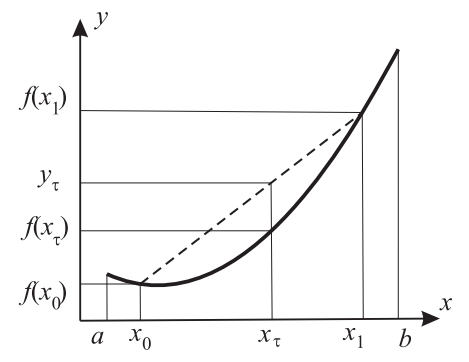
\includegraphics[scale=0.5]{images/img07}
	$$
	То есть для выпуклой функции часть графика выпуклой функции, находящаяся между точками пересечения графика и любой секущей, лежит ниже этой секущей.
	\begin{theorem}
		[Критерий выпуклости дифференцируемой функции]
		Пусть функция $f$ дифференцируема на $|a,b|$. Для выпуклости $f$ на $|a,b|$ необходимо и достаточно, чтобы производная $f'(x)$ была возрастающей функцией на интервале $(a,b)$.
	\end{theorem}
	\begin{theorem}
		[Критерий выпуклости дважды дифференцируемой функции]
		Пусть функция $f$ дважды дифференцируема на $|a,b|$. Для выпуклости $f$ на $|a,b|$ необходимо и достаточно, чтобы
		\begin{equation*}
			f''(x) \geq 0 \quad \forall x \in (a,b).
		\end{equation*}
	\end{theorem}
	\noindent
	{Внутреннюю точку $x_0$ промежутка $[a, b]$ называют точкой:}
	\begin{itemize}
		\item {\textbf{локального максимума} функции $f : [a, b] \to \mathbb{R}$, если}
		\[
		f(x_0) \geq f(x)
		\]
		\textit{для всех $x$ из некоторой $\delta$-окрестности $[x_0 - \delta, x_0 + \delta]$, $\delta > 0$, точки $x_0$;}
		\item {\textbf{локального минимума}, если}
		\[
		f(x_0) \leq f(x) \quad \forall x \in [x_0 - \delta, x_0 + \delta].
		\]
	\end{itemize}
	{Точки локального минимума и локального максимума называют точками \textbf{локального экстремума}}.
	\begin{theorem}
		[Необходимое условие локального экстремума]
		Если $x_0$ -- точка локального экстремума дифференцируемой в точке $x_0$
		функции, то $x_0$ -- стационарная точка функции.
	\end{theorem}
	\noindent
	Точками, подозрительными на локальный экстремум
	непрерывной функции, являются стационарные точки и точки, в которых
	функция не дифференцируема.
	\begin{theorem}
		[Правила исследования стационарных точек]
		\begin{enumerate}
			\item Пусть функция $f(x)$ непрерывно дифференцируема на интервалах $(x_0 - \delta, x_0)$, $(x_0, x_0 + \delta)$ и непрерывна в точке $x_0$, и пусть $x_0$ является либо стационарной точкой функции, либо точкой, в которой функция не дифференцируема. Тогда если при переходе через точку $x_0$ производная $f'(x)$
			\begin{itemize}
				\item меняет знак с <<->> на <<+>>, то $x_0$ — точка локального максимума;
				\item меняет знак с <<+>> на <<->>, то $x_0$ — точка локального минимума;
				\item не меняет знак, то $x_0$ не является точкой экстремума.
			\end{itemize}
			\item Пусть функция $f(x)$ дважды непрерывно дифференцируема в некоторой окрестности стационарной точки $x_0$. Тогда
			\begin{itemize}
				\item если $f''(x_0) > 0$, то $x_0$ — точка локального минимума;
				\item если $f''(x_0) < 0$, то $x_0$ — точка локального максимума.
			\end{itemize} 
			\item Пусть функция $f(x)$ $n$ раз непрерывно дифференцируема в некоторой окрестности точки $x_0$ и 
			\[
			f'(x_0) = f''(x_0) = \dots = f^{(n-1)}(x_0) = 0, \quad f^{(n)}(x_0) \neq 0.
			\]
			Тогда
			\begin{itemize}
				\item если $n$ — чётное и $f^{(n)}(x_0) > 0$, то $x_0$ — точка локального минимума;
				\item если $n$ — чётное и $f^{(n)}(x_0) < 0$, то $x_0$ — точка локального максимума;
				\item если $n$ — нечётное, то $x_0$ не является точкой локального экстремума.
			\end{itemize}  
		\end{enumerate}
	\end{theorem}
	\noindent
	Рассмотрим функцию $f:X\to \mathbb R$. Пусть \begin{equation*}
		\underset{x \in X}{\sup} f(x) = M,\ \underset{x \in X}{\inf} f(x) = m,
	\end{equation*}
	$-\infty < M \leq +\infty$, $-\infty \leq m < +\infty$.
	\\\\
	{Если существует точка $\overline x\in X$ такая, что $f(\overline x) = M$, то $\overline x$ -- это \textbf{точка глобального максимума} и пишут $$M = \underset{x \in X}{\max} f(x).$$
	Если существует точка $\underline x\in X$ такая, что $f(\underline x) = m$, то $\underline x$ -- это \textbf{точка глобального минимума} и пишут} $$m = \underset{x \in X}{\min} f(x).$$
	Укажем способ нахождения глобальных экстремумов непрерывной функции $f$ в двух случаях: 1) $X$ — отрезок $[a, b]$, 2) $X$ — интервал $(a, b)$.
	\\\\
	В первом случае допустим, что $f$ имеет конечное число точек $\xi_1, \dots, \xi_l$, подозрительных на точки локального экстремума, принадлежащих интервалу $(a, b)$. Для выявления точек глобального экстремума достаточно найти значения функции $f(\xi_1), \dots, f(\xi_l)$ и сравнить их со значениями $f(a)$ и $f(b)$:
	\[
	M = \max\{f(\xi_1), \dots, f(\xi_l), f(a), f(b)\},
	\]
	\[
	m = \min\{f(\xi_1), \dots, f(\xi_l), f(a), f(b)\}.
	\]
	Во втором случае допустим, что $f$ имеет конечное число точек $\xi_1, \dots, \xi_l$, подозрительных на точки локального экстремума, принадлежащих интервалу $(a, b)$, и существуют (конечные или бесконечные) пределы
	\[
	\lim_{x \to a+0} f(x) = f(a + 0), \quad \lim_{x \to b-0} f(x) = f(b - 0).
	\]
	Вычислим значения функции $f(\xi_1), \dots, f(\xi_l)$. Если
	\[
	\max\{f(\xi_1), \dots, f(\xi_l)\} = f(\xi_i) \geq \max\{f(a + 0), f(b - 0)\},
	\]
	то $\xi_i$ — точка глобального максимума, если
	\[
	\max\{f(a + 0), f(b - 0)\} > \max\{f(\xi_1), \dots, f(\xi_l)\},
	\]
	то $f$ не достигает глобального максимума на $(a, b)$ и
	\[
	\sup_{x \in X} f(x) = \max\{f(a + 0), f(b - 0)\}.
	\]
	Аналогично находятся точки глобального минимума.
	\begin{theorem}
		[о глобальном минимуме выпуклой функции]
		Если $f$ -- дифференцируемая выпуклая (вогнутая) функция на интервале $(a,b)$ и $x_0 \in (a,b)$ -- ее стационарная точка, то $x_0$ -- точка глобального минимума (максимума), то есть 
		$$f(x_0) = \underset{x \in (a,b)}{\min}f(x)\quad (f(x_0) = \underset{x \in (a,b)}{\max}f(x)).$$
	\end{theorem}
	\noindent
	Пусть $D\subseteq\mathbb R^2$. 
	\\\\
	{Функцию $f:D \to \mathbb R$ называют \textbf{функцией двух переменных} и обозначают $z = f(x,y)$.}
	\\\\
	Рассмотрим соотношение
	\begin{equation}
		F(x,y) = 0.
	\end{equation}
	Ппусть существует прямоугольник $\Pi = [a,b]\times [c,d]$.
	\\\\
	{Если функция $y=\varphi(x)$, определенная на отрезке $[a,b]$, каждому $x \in [a,b]$ ставит в соответствие единственное число $y \in [c,d]$ такое, что $F(x,y) = 0$, то такая функция называется \textbf{неявной}, заданной соотношением $F(x,y) = 0$ в прямоугольнике $\Pi$.}
	\begin{theorem}
		[о неявной функции]
		Пусть $F(x,y)$ удовлетворяет условиям:
		\begin{enumerate}
			\item существует точка $(x_0, y_0)\in D$ такая, что $F(x_0, y_0) = 0$;
			\item непрерывно дифференцируема в некоторой окрестности точки $(x_0, y_0)$;
			\item $F'y(x_0,y_0)\ne 0$.
		\end{enumerate}
		Тогда существует прямоугольник
		\begin{equation*}
			\Pi = \{(x,y) : x_0 -a \leq x \leq x_0 + a,\ y_0 - b\leq y \leq y_0+b\},\ a>0,\ b>0,
		\end{equation*}
		в котором соотношение $F(x,y)=0$ задает непрерывно дифференцируемую неявную функцию $y = \varphi(x)$, производная которой равна
		\begin{equation}
			\varphi'(x) = -\dfrac{F'_x(x,\varphi(x))}{F'_y(x,\varphi(x))},\ \forall x \in [x_0-a,\ x_0+a].
		\end{equation}
	\end{theorem}
	\noindent
	Рассмотрим множество $E \subseteq \mathbb R$. Пусть на $E$ задана последовательность скалярных функций $(f_n(x))$ таких, что $f_n:E \to \mathbb R$. 
	\\\\
	{Сумма $\sum_{n=1}^\infty f_n(x)$, $x \in E$ называется \textbf{функциональным рядом}. Множество $E^*$ таких $x\in E$, при которых ряд $\sum_{n=1}^\infty f_n(x)$ сходится, называется \textbf{множеством сходимости} функционального ряда.}
	\\\\
	Пусть функция $S_n(x) = \sum_{k=1}^n f_k(x)$ -- это частная сумма ряда. 
	\\\\
	{Функциональный ряд $\sum_{n=1}^\infty f_n(x)$ называется \textbf{равномерно сходящимся на $E^*$ к функции $S(x)$}, если}
	\begin{equation}
		\forall \epsilon > 0,\ \exists \delta > 0: \forall n \geq \delta\ \forall x \in E^* \Rightarrow|S_n(x) - S(x) | \leq\ \epsilon.
	\end{equation}
	Таким образом, функция может быть задана через равномерно сходящийся функциональный ряд
	\begin{equation}
		S(x) = \sum_{n=1}^\infty f_n(x),\ x \in E^*.
	\end{equation}
	\begin{theorem}
		[Стокса-Зейделя о непрерывности суммы ФР]
		Если
		\begin{itemize}
			\item члены $f_n(x)$ функционального ряда $\sum_{n=1}^\infty f_n(x)$ непрерывны на отрезке $[a,b]$;
			\item ряд $\sum_{n=1}^\infty f_n(x)$ сходится равномерно на $[a,b]$,
		\end{itemize} 
		то функция $S(x) = \sum_{n=1}^\infty f_n(x)$ непрерывна на $[a,b]$.
	\end{theorem}
	\begin{theorem}
		[о почленном интегрировании ФР]
		Если 
		\begin{itemize}
			\item члены $f_n(x)$ функционального ряда $\sum_{n=1}^\infty f_n(x)$ непрерывны на отрезке $[a,b]$;
			\item ряд $\sum_{n=1}^\infty f_n(x)$ сходится равномерно на $[a,b]$,
		\end{itemize} 
		то его можно почленно интегрировать на любом отрезке $[\alpha, \beta]\subset [a,b]$
		\begin{equation}
			\int\limits_\alpha^\beta S(x)dx = \int\limits_\alpha^\beta \left( \sum_{n=1}^\infty f_n(x)\right)dx = \sum_{n=1}^\infty \left(\int\limits_\alpha^\beta f_n(x) dx \right).
		\end{equation}
	\end{theorem}
	\begin{theorem}
		[о почленном дифференцировании ФР]
		Если
		\begin{itemize}
			\item ряд $\sum_{n=1}^\infty f_n(x)$ сходится поточечно на $[a,b]$;
			\item члены $f_n(x)$ функционального ряда $\sum_{n=1}^\infty f_n(x)$ непрерывно дифференцируемы на отрезке $[a,b]$;
			\item ряд из производных $\sum_{n=1}^\infty f_n'(x)$ сходится равномерно на $[a,b]$,
		\end{itemize}
		то функциональный ряд можно почленно дифференцировать
		\begin{equation}
			S'(x) = \left(\sum_{n=1}^\infty f_n(x)\right)' = \sum_{n=1}^\infty f_n'(x),\ x \in [a,b].
		\end{equation}
	\end{theorem}
	\noindent 
	Таким образом, функции могут быть заданы в виде равномерно сходящихся функциональных рядов, при этом они будут обладать свойствами непрерывности, интегрируемости и дифференцируемости.\\\\
	К примеру, основные элементарные функции могут быть представлены в окрестности некоторой точки $x_0$ в виде степенного ряда Тейлора
	\begin{equation}
		f(x) = \sum_{n=0}^\infty \dfrac{f{(n)}}{n!}(x-x_0)^n,
	\end{equation}
	причем такое разложение единственно.
	\\\\
	Рассмотрим скалярную функцию двух переменных, определенную на множестве $[a,b)\times Y$, $Y \subseteq \mathbb R$. Пусть при каждом фиксированном $y \in Y$ функция $f(x,y)$ интегрируема на $[a,b)$. 
	\\\\
	{На множестве $Y$ определена функция 
		\begin{equation}
			F(y) = \int\limits_a^b f(x,y)dx,
		\end{equation}
		которую называют \textbf{интегралом, зависящим от параметра}.}
	\\\\
	Рассмотрим функцию $f(x,y)$ заданную на множестве $X \times Y$. Пусть $y_0$ -- это предельная точка множества $Y$ и пусть для каждого фиксированного $x\in X$ существует предел
	\begin{equation}
		\lim\limits_{y \to y_0,\ y \in Y} f(x,y) = \varphi(x)
	\end{equation}
	вдоль множества $Y$. 
	{Тогда функция $\varphi(x)$ называется \textbf{предельной функцией} для $f(x,y)$ при $y \to y_0$ вдоль $Y$, а сходимость называется \textbf{поточечной}.}
	\\\\
	{Если 
		\begin{equation}
			\forall \epsilon > 0,\ \exists \delta > 0,\ \forall y \in Y : 0 < |y-y_0|<\delta,\ \forall x \in X \Rightarrow |f(x,y) - \varphi(x) | \leq \epsilon,
		\end{equation}
		то функция $f(x,y)$ \textbf{равномерно сходится} к $\varphi(x)$ на множестве $X$ при $y \to y_0$.}
	\begin{theorem}
		[о переходе к пределу под знаком интеграла]
		Если 
		\begin{itemize}
			\item при каждом фиксированном $y \in Y$ функция $f(x,y)$ непрерывна по $x$ на отрезке $[a,b]$;
			\item $f(x,y) \underset{y\to y_0}{\overset{[a,b]}{\rightrightarrows}}\varphi(x)$,
		\end{itemize} то
		\begin{equation}
			\lim\limits_{y \to y_0} F(y) = \lim\limits_{y \to y_0}\int\limits_a^b f(x,y)dx = \int\limits_a^b\lim\limits_{y \to y_0} f(x,y)dx = \int\limits_a^b \varphi(x)dx.
		\end{equation}
	\end{theorem}
	\begin{theorem}
		[о непрерывности ИЗОП]
		Если функция $f(x,y)$ непрерывна на прямоугольнике $[a,b]\times [c,d]$, то функция 
		\begin{equation*}
			F(y) = \int\limits_a^b f(x,y)dx,
		\end{equation*}
		непрерывна на $[c,d]$.
	\end{theorem}
	\begin{theorem}
		[о дифференцировании ИЗОП]
		Пусть
		\begin{itemize}
			\item функция $f(x,y)$ непрерывна по $x$ при каждом фиксированном $y \in [c,d]$;
			\item частная производная $f'y(x,y)$ непрерывна на $[a,b]\times [c,d]$.
		\end{itemize}
		Тогда имеет место формула Лейбница
		\begin{equation}
			F'(y) = \left(\int\limits_a^b f(x,y)dx\right)'  = \int\limits_a^b f'_y(x,y)dx\ \forall y \in [c,d].
		\end{equation}
	\end{theorem}
	\begin{theorem}
		[о перестановке порядка интегрирования]
		Если функция $f(x,y)$ непрерывна на прямоугольнике $[a,b]\times [c,d]$, то \begin{equation}
			\int\limits_c^d dy \int\limits_a^b f(x,y)dx = \int\limits_a^b dx \int\limits_c^d f(x,y)dy.
		\end{equation}
	\end{theorem}
	
	\section{Интегралы}
	Пусть на отрезке $[a,b]$ задана функция $y=f(x)$. Возьмем разбиение отрезка $[a,b]$ на $n$ частей
	\begin{equation*}
		a = x_0 < x_1 < \ldots < x_{n-1} < x_n = b.
	\end{equation*}
	Обозначим $\Delta x_k = x_k - x_{k-1}$. 
	\\\\
	Число $\delta (\{x_k\}) = \underset{k}{\max} \Delta x_k$ называется \textbf{диаметром разбиения}.
	\\\\
	На каждом отрезке $[x_{k-1}, x_k]$ выбираем точку $\xi _k$ и строим интегральную сумму
	\begin{equation}
		\sigma(\{x_k\}, \xi_k) = \sum_{k=1}^n f(\xi_k)\Delta x_k.
	\end{equation}
	Значение интегральной суммы зависит от способа разбиения отрезка $[a,b]$ и выборка точек $\xi_k$. 
	$$
	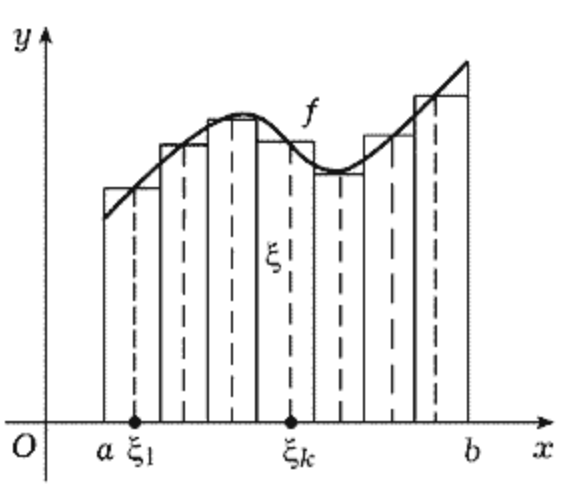
\includegraphics[scale=0.4]{images/img08}
	$$
	Мы можем выбрать сколь угодно малый диаметр разбиения, то есть $\delta (\{x_k\}) \to 0$. В таком случае
	\begin{equation*}
		\forall \epsilon > 0,\ \exists \delta > 0,\ \forall \{x_k\} : \delta (\{x_k\}) \leq \delta,\ \forall \xi_k \Rightarrow |\sigma(\{x_k\}, \xi_k) - I| \leq \epsilon,
	\end{equation*}
	то есть
	\begin{equation*}
		\sigma(\{x_k\}, \xi_k) = \sum_{k=1}^n f(\xi_k)\Delta x_k \xrightarrow[ \delta (\{x_k\}) \to 0]{м} \int\limits_a^b f(x)dx = I.
	\end{equation*}
	Число $I$ называется интегралом Римана от функции $f(x)$ на отрезке $[a,b]$, а функцию $f(x)$ называют \textbf{интегрируемой по Риману} на отрезке $[a,b]$.
	\begin{theorem}
		[Необходимое условие интегрируемости по Риману]
		Если функция $f(x)$ интегрируема по Риману на отрезке $[a,b]$, то она ограничена.
	\end{theorem}
	\noindent
	Рассмотрим основные методы вычисления интегралов Римана
	\begin{enumerate}
		\item \textbf{Формула Ньютона-Лейбница}
		\begin{equation}
			\int\limits_a^b f(x)dx = F(x)\Big|_a^b= F(b) - F(a),
		\end{equation}
		где $F(x) = \int f(x)dx$ -- это первообразная.
		\item \textbf{Формула замены переменной.} Если $f:[a,b] \to \mathbb R$ -- непрерывная функция, а $\varphi : [\alpha, \beta]\to [a,b]$ -- непрерывно дифференцируемое отображение такое, что $\varphi(\alpha) = a$, $\varphi(\beta) = b$, то имеет место формула
		\begin{equation}
			\int\limits_a^b f(x)dx = \int\limits_\alpha^\beta f(\varphi(t))\cdot \varphi'(t)dt.
		\end{equation}
		\item \textbf{Формула интегрирования по частям.} Пусть $u(x)$, $v(x)$ -- непрерывно дифференцируемые на отрезке $[a,b]$ функции. Тогда
		\begin{equation}
			\int\limits_a^b u(x)v'(x)dx = u(x)v(x)\Big|_a^b - \int\limits_a^b v(x)u'(x)dx.
		\end{equation}
	\end{enumerate}
	Интеграл Римана позволяет вычислять площадь под графиком кривой и длины кривых, заданных параметрически.
	\\\\
	Интеграл Римана и интеграл Лебега отличаются подходом к тому, как «суммировать» значения функции, и тем, какие функции можно интегрировать.
	\begin{enumerate}
		\item \textbf{Разбиение области интегрирования:}
		\begin{itemize}
			\item При Римановом интегрировании область определения функции (ось $x$) разбивается на маленькие интервалы, и интеграл рассчитывается как предел суммы прямоугольников, высота которых задаётся значениями функции на этих промежутках. Таким образом, вся схема построена на разбиении по $x$.
			\item В случае интеграла Лебега акцент смещается с разбиения области $x$ на разбиение по значениям функции (ось $y$). То есть мы группируем точки, где функция принимает похожие значения, и суммируем вклад каждого такого «слоя», умножая его на меру (объём в смысле меры) множества, где функция примерно равна этому значению.
		\end{itemize}
		\item \textbf{Класс интегрируемых функций:}
		\begin{itemize}
			\item Подход Римана хорошо работает для функций, которые «не слишком разрывны» и имеют «хорошее» поведение на отрезке. Если функция имеет слишком много разрывов или обладает сложной структурой, Риманов интеграл может не существовать.
			\item Лебегов интеграл способен обрабатывать гораздо более широкий класс функций, поскольку он оперирует с измеримыми функциями. Даже если функция сильно разрывна, но её значение можно «сгруппировать» по известным измеримым множествам, интеграл Лебега может существовать.
		\end{itemize}
	\end{enumerate}
	Лебегов интеграл обладает мощными теоремами сходимости, что позволяет уверенно переходить к пределу последовательностей функций. Это особенно важно в анализе и в теории вероятностей.
	\\\\
	Например, пусть задано измеримое вероятностное пространство $(\Omega, \mathcal F, \mathbf P)$, где $\Omega$ -- пространство элементарных событий, $\mathcal F$ -- $\sigma$-алгебра, $\mathbf P$ -- вероятностная мера, на котором определена случайная величина $X : \Omega \to \mathbb R$, которая является измеримой функцией. Если существует интеграл Лебега от $X$ по пространству $\Omega$, то он называется \textbf{математическим ожиданием}
	\begin{equation}
		\mathbb E \{X\} = \int\limits_\Omega X(\omega) P(d\omega).
	\end{equation}
	В теории вероятностей эта характеристика играет огромную роль при исследовании случайных величин.
	\\\\
	Рассмотрим скалярную функцию $y = f(x)$, заданную на промежутке $[a, +\infty)$ и интегрируемую по Риману на любом отрезке $[a, A], \, A > a$. Построим функцию
	$$
	F(A) = \int\limits_a^A f(x) \, dx, \ A \in [a, \infty).
	$$
	Предел функции $F(A)$ при $A \to \infty$ называют \textbf{несобственным интегралом первого типа} (НИ-1) от функции $f(x)$ по промежутку $[a, +\infty)$ и обозначают
	$$
	\int\limits_a^{+\infty} f(x) \, dx = \lim\limits_{A \to \infty} F(A) = \lim\limits_{A \to \infty} \int\limits_a^A f(x) \, dx.
	$$
	Если предел $\lim\limits_{A \to \infty} F(A)$ конечен, то несобственный интеграл называют \textbf{сходящимся}, а функцию $f(x)$ — \textbf{интегрируемой} (в несобственном смысле) на $[a, +\infty)$. В противном случае, если предел $\lim\limits_{A \to \infty} F(A)$ либо не существует, либо равен $\infty$, то интеграл называют \textbf{расходящимся}.
	\\\\
	Если $f(x)$ при $x \geq a$ неотрицательная и непрерывная функция, то $\int_a^A f(x) \, dx$ равен площади криволинейной трапеции, ограниченной осью $Ox$, прямыми $x = a$, $x = A$ и графиком функции $y = f(x)$. В случае сходимости интеграла $\int_a^{+\infty} f(x) \, dx$ его значение естественно принять за площадь неограниченной фигуры, заключённой между осью $Ox$, прямой $x = a$ и графиком функции $f(x)$
	$$
	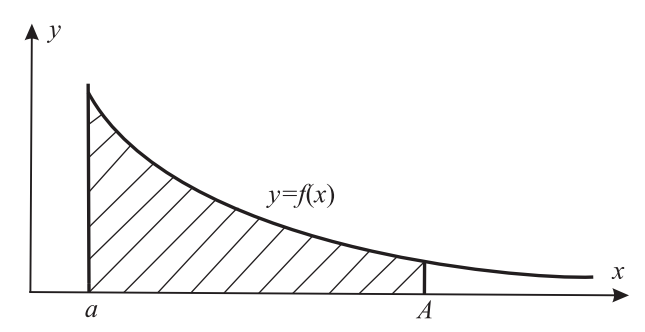
\includegraphics[scale=0.5]{images/img09}
	$$
	Рассмотрим функцию $y=f(x)$, заданную на промежутке $[a, b)$. Предположим, точка $b$ такова, что на любом отрезке $[a, b - \eta]$, $0 < \eta < b - a$, функция интегрируема по Риману, но не интегрируема на отрезке $[a, b]$. Точку $x = b$ с такими свойствами называют \textbf{особой точкой} функции $f$.
	\\\\
	Предел
	\[
	\int\limits_a^b f(x) \, dx = \lim\limits_{\eta \to +0} \int\limits_a^{b - \eta} f(x) \, dx \tag{16.6}
	\]
	называют \textbf{несобственным интегралом второго типа} (НИ-2) от функции $f(x)$ на промежутке $[a, b)$ и обозначают
	$$
	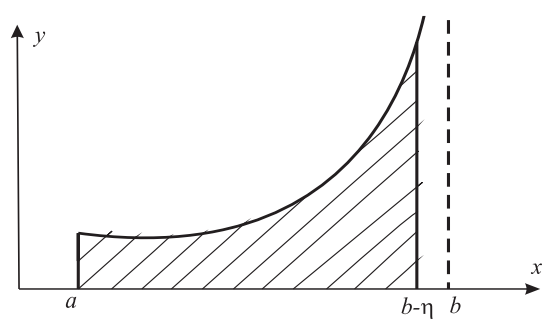
\includegraphics[scale=0.5]{images/img10}
	$$
	Если предел конечен, то несобственный интеграл второго типа называют \textbf{сходящимся}, а функцию $f$ — интегрируемой (в несобственном смысле) на $[a, b]$. В противном случае говорят, что интеграл \textbf{расходится}.
	\\\\
	Пусть теперь функция интегрируема по Риману на любом отрезке $[a + \eta, b]$, $0 < \eta < b - a$, но не интегрируема на $[a, b]$. В этом случае говорят, что точка $x = a$ — особая. Несобственный интеграл второго типа на промежутке $(a, b]$ определяют равенством
	\[
	\int\limits_a^b f(x) \, dx = \lim\limits_{\eta \to +0} \int\limits_{a + \eta}^b f(x) \, dx.
	\]
	Для вычисления несобственных интегралов 1-го и 2-го типов используются
	\begin{itemize}
		\item формула Ньютона-Лейбница;
		\item замена переменных;
		\item формула интегрирования по частям.
	\end{itemize}
	Всякую совокупность точек $T \subset \mathbb R^n$ называют \textbf{телом}.
	Совокупность тел $\{T_k\} = \{T_1, \ldots, T_n\}$ называют \textbf{разбиением} тела $T$, если объединение всех $T_k$ составляет $T$ и никакие две части из $\{T_k\}$ не имеют общих внутренних точек. Если $\{T_k\}$ — разбиение $T$, то
	\[
	\text{об.} T = \sum_{k=1}^n \text{об.} T_k.
	\]
	Величину
	\[
	\delta(\{T_k\}) = \max_{1 \leq k \leq n} \{\text{diam} T_k\}, \quad \text{где } \text{diam} T_k = \sup_{\mathbf{x}_1, \mathbf{x}_2 \in T_k} \rho(\mathbf{x}_1, \mathbf{x}_2),
	\]
	называют \textbf{диаметром разбиения}.
	\\\\
	Допустим, что задана функция $f : T \to \mathbb{R}$. Возьмем разбиение $\{T_k\}$ тела $T$ на $n$ частей и выберем по точке $\mathbf{x}_k \in T_k$. Построим \textbf{интегральную сумму}
	\[
	\sigma = \sum_{k=1}^n f(\mathbf{x}_k) \, \text{об.} T_k.
	\]
	Если существует число $I$ такое, что
	\[
	\forall \varepsilon > 0, \, \exists \delta(\varepsilon) > 0, \, \forall \{T_k\} : \delta(\{T_k\}) \leq \delta(\varepsilon), \, \forall \mathbf{x}_k \in T_k \implies |\sigma - I| \leq \varepsilon,
	\]
	то функцию $f$ называют \textbf{интегрируемой по Риману на $T$}, а число $I$ — \textbf{$n$-кратным интегралом} от $f$ по $T$ и обозначают
	\[
	\int_T f(x) \, dx \quad \text{или} \quad \int_T \ldots \int f(x_1, \ldots, x_n) \, dx_1 \ldots dx_n.
	\]
	Тело $T = \{(x_1, \ldots, x_{n-1}, x_n) : (x_1, \ldots, x_{n-1}) \in D, \psi_1(x_1, \ldots, x_{n-1}) \leq x_n \leq \psi_2(x_1, \ldots, x_{n-1})\}$,  
	где $D$ — замкнутая ограниченная область в $\mathbb{R}^{n-1}$,  
	а $\psi_1(x_1, \ldots, x_{n-1})$, $\psi_2(x_1, \ldots, x_{n-1})$ — непрерывные на $D$ функции, называют \textbf{цилиндроидом}, элементарным относительно оси $0x_n$.
	\begin{theorem}
		[о сведении кратного интеграла к повторному интегралу]
		Пусть $T$ — цилиндроид, элементарный относительно оси $0x_n$, и пусть $f(x_1, \ldots, x_n)$ — непрерывная на $T$ функция. Тогда
		\[
		\int_T \cdots \int f(x_1, \ldots, x_n) \, dx_1 \cdots dx_n =
		\int_D \cdots \int dx_1 \cdots dx_{n-1} \int\limits_{\psi_1(x_1, \ldots, x_{n-1})}^{\psi_2(x_1, \ldots, x_{n-1})} f(x_1, \ldots, x_n) \, dx_n.
		\]
	\end{theorem}
	\noindent
	Особенность заключается в том, что $n$-кратные интегралы позволяют вычислять объемы $n$-мерных тел.
	\\\\
	Пусть $l^+$ -- это кусочно-гладкий путь
	\begin{equation*}
		l: \begin{cases}
			x = x(t),\\
			y = y(t);
		\end{cases} t \in [a,b],
	\end{equation*}
	$x(t)$, $y(t)$ -- непрерывные на $[a,b]$ функции. 
	Пусть задана функция $f: D \to \mathbb R$, $D \subset \mathbb R^2$, $l\subset D$ такая, что отображение $f(x(t), y(t))$ интегрируемо по Риману на $[a,b]$. Тогда функция $f(x(t), y(t))\cdot \sqrt{\dot x^2 (t) + \dot y^2 (t)}$ также интегрируема по Риману на $[a,b]$ в силу интегрируемости $f(x(t), y(t))$ и 
	\begin{equation*}
		\text{дл}.l = \int\limits_a^b\sqrt{\dot {x} ^2 (t) + \dot {y}^2 (t)} dt.
	\end{equation*}
	Интеграл Римана вида
	\begin{equation}
		\int\limits_a^b f(x(t), y(t))\cdot \sqrt{\dot {x} ^2 (t) + \dot {y}^2 (t)} dt = \int\limits_{l^+} f(x,y)ds
	\end{equation}
	называется \textbf{криволинейным интегралом первого типа} от $f(x,y)$ по пути $l^+$.
	\begin{itemize}
		\item \textbf{Механический смысл.} Если $f(x,y)$ -- это линейная плотность пути $l^+$, то $\int\limits_{l^+} f(x,y)ds$ определяет массу пути.
		\item \textbf{Экономический смысл.} Если $f(x,y)$ -- это удельная стоимость провоза груза в точке $(x,y)$ по пути $l^+$, то $\int\limits_{l^+} f(x,y)ds$ определяет цену провоза груза по всему пути.
	\end{itemize}
	Пусть заданы две функции $P(x,y)$, $Q(x,y)$, определенные на $D$ такие, что $P(x(t), y(t))$, $Q(x(t), y(t))$ интегрируемы по Риману на отрезке $[a,b]$. Тогда $P(x(t), y(t))\cdot \dot x (t)$, $Q(x(t), y(t))\cdot \dot y(t)$ также интегрируемы по Риману на отрезке $[a,b]$, а интегралы Римана вида
	\begin{equation}
		\int\limits_a^bP(x(t), y(t))\cdot \dot x (t)dt = \int\limits_{l^+} P(x,y)dx,\ \int\limits_a^bQ(x(t), y(t))\cdot \dot y (t)dt = \int\limits_{l^+} Q(x,y)dy
	\end{equation}
	называются \textbf{криволинейными интегралами второго типа} соответственно от функций $P(x,y)$, $Q(x,y)$ по пути $l^+$.
	Чаще всего рассматривается сумма этих интегралов, которая обозначается
	\begin{equation}
		\int\limits_{l^+} P(x,y)dx + Q(x,y)dy.
	\end{equation}
	\begin{itemize}
		\item \textbf{Механический смысл.} Если задано силовое поле $\mathbf F = P(x,y)\cdot \mathbf i + Q(x,y)\cdot \mathbf j$, то $\int\limits_{l^+} P(x,y)dx + Q(x,y)dy$ определяет работу силы $\mathbf F$ по перемещению точки единичной массы по пути $l^{+}$.
		\item \textbf{Применение.} КРИ-2 в совокупности с теоремой о независимости КРИ-2 от формы пути определяет метод решения обыкновенных дифференциальных уравнений в полных дифференциалах.
	\end{itemize}
	\begin{theorem}
		[о сведении КРИ-2 к 2И]
		Пусть $D$ — ограниченная замкнутая область, граница которой является простой кусочно-гладкой кривой $\partial D$, а $P(x, y)$ и $Q(x, y)$ — непрерывно дифференцируемые на $D$ функции. Тогда справедлива \textbf{формула Грина}
		\[
		\int_{\partial D^+} \big(P(x, y) \, dx + Q(x, y) \, dy\big) = \iint_D \left(\frac{\partial Q}{\partial x} - \frac{\partial P}{\partial y}\right) dx \, dy,
		\]
		где $\partial D^+$ — путь, находящийся на границе фигуры $D$ и ориентированный таким образом, что при движении по пути в этом направлении, фигура остается слева 
	\end{theorem}
	Пусть $w = f(x, y, z)$ — скалярная функция, заданная на множестве $E \subset \mathbb{R}^3$, а
	\[
	S: 
	\begin{cases}
		x = x(u, v), \\
		y = y(u, v), \\
		z = z(u, v),
	\end{cases}
	\quad (u, v) \in \overline{D},
	\]
	— кусочно-гладкая поверхность, лежащая в $E$. Предположим, что функция 
	$f(x(u, v), y(u, v), z(u, v))$ интегрируема по Риману на $\overline{D}$. Отображение
	\[
	\sqrt{E((u, v))G((u, v)) - F^2((u, v))}, \quad (u, v) \in \overline{D},
	\]
	ограничено и имеет множество точек разрыва нулевой площади, следовательно, оно тоже интегрируемо по Риману на $\overline{D}$. Функция $f(x(u, v), y(u, v), z(u, v))\sqrt{EG - F^2}$ интегрируема на 
	$\overline{D}$ как произведение интегрируемых функций.
	\\\\
	Двойной интеграл вида
	\[
	\iint\limits_{\overline{D}} f(x(u, v), y(u, v), z(u, v)) \sqrt{EG - F^2} \, dudv
	\]
	принимают за \textbf{поверхностный интеграл первого типа} от $f$ по поверхности $S$ (ПОВИ-1) и обозначают
	\[
	\iint\limits_{S} f(x, y, z) \, ds.
	\]
	Таким образом, по определению
	\[
	\iint\limits_{S} f(x, y, z) \, ds := \iint\limits_{\overline{D}} f(x(u, v), y(u, v), z(u, v)) \sqrt{EG - F^2} \, dudv.
	\]
	\textbf{Физический смысл.} Если $\rho(x,y,z)$ -- плотность простой кусочно-гладкой поверхности $S$ в точке $(x,y,z)$, то ПОВИ-1 $\iint\limits_{S} \rho(x, y, z) \, ds$ равен массе поверхности $S$.
	\\\\
	Пусть на множестве $E \subset \mathbb{R}^3$ заданы три скалярные функции 
	$P(x, y, z)$, $Q(x, y, z)$, $R(x, y, z)$ и пусть $S^+ = (S, \mathbf{q})$ — положительная сторона 
	простой гладкой поверхности, $S \subset E$.
	\\\\
	Поверхностные интегралы первого типа
	\[
	\iint\limits_{S} P(x, y, z) \cos (\mathbf{q} \mathbf{i}) \, ds, \quad 
	\iint\limits_{S} P(x, y, z) \cos (-\mathbf{q} \mathbf{i}) \, ds,
	\]
	\[
	\iint\limits_{S} Q(x, y, z) \cos (\mathbf{q} \mathbf{j}) \, ds, \quad 
	\iint\limits_{S} Q(x, y, z) \cos (-\mathbf{q} \mathbf{j}) \, ds,
	\]
	\[
	\iint\limits_{S} R(x, y, z) \cos (\mathbf{q} \mathbf{k}) \, ds, \quad 
	\iint\limits_{S} R(x, y, z) \cos (-\mathbf{q} \mathbf{k}) \, ds,
	\]
	относят к \textbf{поверхностным интегралам второго типа} (ПОИП-2) и обозначают соответственно
	\[
	\iint\limits_{S^+} P(x, y, z) \, dy dz, \quad 
	\iint\limits_{S^-} P(x, y, z) \, dy dz, \quad 
	\iint\limits_{S^+} Q(x, y, z) \, dx dz, \quad 
	\iint\limits_{S^-} Q(x, y, z) \, dx dz,
	\]
	\[
	\iint\limits_{S^+} R(x, y, z) \, dx dy, \quad 
	\iint\limits_{S^-} R(x, y, z) \, dx dy.
	\]
	Чаще всего рассматривают сумму интегралов 
	\[
	\iint\limits_{S^+} P \, dz dy + \iint\limits_{S^+} Q \, dx dz + \iint\limits_{S^+} R \, dx dy,
	\]
	которую обозначают следующим образом:
	\[
	\iint\limits_{S^+} P \, dz dy + Q \, dx dz + R \, dx dy.
	\]
	\begin{theorem}
		[о сведении ПОВИ-2 к тройному интегралу]
		Пусть граница $\partial T$ ограниченной замкнутой области $T \subset \mathbb{R}^3$ является 
		простой кусочно-гладкой поверхностью и пусть $P(x, y, z)$, $Q(x, y, z)$, $R(x, y, z)$ — 
		скалярные непрерывно дифференцируемые на $T$ функции. Тогда имеет место формула Гаусса — Остроградского
		\[
		\iint\limits_{\partial T^+} P \, dzdy + Q \, dxdz + R \, dxdy = 
		\iiint\limits_{T} \left(P'_x + Q'_y + R'_z \right) \, dxdydz,
		\]
		где $\partial T^+$ — внешняя сторона границы тела $T$.
	\end{theorem}
	
	\section{Функциональные последовательности и ряды}
	Рассмотрим множество $E \subseteq \mathbb R$. Пусть на $E$ задана последовательность скалярных функций $(a_n(x))$ таких, что $a_n:E \to \mathbb R$. 
	\\\\
	Если при каждом фиксированном $x \in E$ 
	\begin{equation*}
		a(x) = \lim\limits_{n\to\infty} a_n(x)
	\end{equation*}
	или же
	\begin{equation*}
		\forall  x \in E,\ \forall \epsilon > 0,\ \exists \delta(x) > 0 : \forall n \geq \delta(x) \Rightarrow |a_n(x) - a(x)| \leq \epsilon, 
	\end{equation*}
	то $a_n(x)$ \textbf{поточечно сходится} к $a(x)$ на $E$. Обозначается \begin{equation*}
		a_n(x) \xrightarrow[n\to\infty]{E} a(x).
	\end{equation*} 
	В таком случае функция $a(x)$ называется \textbf{предельной функцией}.
	Если выполняется более сильное условие
	\begin{equation*}
		\forall \epsilon > 0,\ \exists \delta > 0 : \forall n \geq \delta,\ \forall x \in E \Rightarrow|a_n(x) - a(x)|\leq \epsilon,
	\end{equation*}
	то $a_n(x)$ \textbf{равномерно сходится} к $a(x)$ на $E$. Обозначается
	\begin{equation*}
		a_n(x) \underset{n\to \infty}{\overset{E}{\rightrightarrows}} a(x).
	\end{equation*}
	Если функциональная последовательность сходится равномерно, то только к предельной функции.
	\begin{theorem}
		[критерий равномерной сходимости ФП]
		$a_n(x) \underset{n\to \infty}{\overset{E}{\rightrightarrows}} a(x)$ тогда и только тогда, когда $\lim\limits_{n\to\infty}\underset{x \in E}{\sup}|a_n(x) - a(x)| = 0$.
	\end{theorem}
	\noindent
	К примеру, функциональная последовательность $a_n(x) = x^n$ на $E = [0,1)$ сходится поточечно к 0, но не равномерно.
	\\\\
	Сумма $\sum_{n=1}^\infty a_n(x)$, $x \in E$ называется \textbf{функциональным рядом}. Множество $E^*$ таких точек $x\in E$, что при каждом $x \in E^*$ ряд $\sum_{n=1}^\infty a_n(x)$ сходится, называется \textbf{множеством поточечной сходимости} функционального ряда.
	\\\\
	Пусть функция $S_n(x) = \sum\limits_{k=1}^n a_k(x)$ -- это частная сумма ряда. 
	\\\\
	Функциональный ряд $\sum\limits_{n=1}^\infty a_n(x)$ называется \textbf{равномерно сходящимся на $E^*$ к функции $S(x)$}, если последовательность частных сумм $S_n(x)$ сходится равномерно к $S(x)$, то есть
	\begin{equation*}
		\forall \epsilon > 0,\ \exists \delta > 0: \forall n \geq \delta\ \forall x \in E^* \Rightarrow|S_n(x) - S(x) | \leq\ \epsilon.
	\end{equation*}
	\begin{theorem}
		[критерий равномерной сходимости ФР]
		Ряд $\sum_{n=1}^{\infty} a_n(x)$ сходится равномерно на $E^*$ тогда и только тогда, когда
		\begin{equation*}
			\lim\limits_{n\to\infty}\underset{x \in E^*}{\sup}\left|\sum\limits_{k=n+1}^\infty a_n(x)\right| = 0.
		\end{equation*}
	\end{theorem}
	\begin{theorem}
		[Стокса-Зейделя о непрерывности суммы ФР]
		Если
		\begin{itemize}
			\item члены $a_n(x)$ функционального ряда $\sum_{n=1}^\infty a_n(x)$ непрерывны на отрезке $[a,b]$;
			\item ряд $\sum_{n=1}^\infty a_n(x)$ сходится равномерно на $[a,b]$,
		\end{itemize} 
		то функция $S(x) = \sum_{n=1}^\infty a_n(x)$ непрерывна на $[a,b]$.
	\end{theorem}
	\begin{theorem}
		[о почленном интегрировании ФР]
		Если 
		\begin{itemize}
			\item члены $a_n(x)$ функционального ряда $\sum_{n=1}^\infty a_n(x)$ непрерывны на отрезке $[a,b]$;
			\item ряд $\sum_{n=1}^\infty a_n(x)$ сходится равномерно на $[a,b]$,
		\end{itemize} 
		то его можно почленно интегрировать на любом отрезке $[\alpha, \beta]\subset [a,b]$
		\begin{equation}
			\int\limits_\alpha^\beta S(x)dx = \int\limits_\alpha^\beta \left( \sum_{n=1}^\infty a_n(x)\right)dx = \sum_{n=1}^\infty \left(\int\limits_\alpha^\beta a_n(x) dx \right).
		\end{equation}
	\end{theorem}
	\begin{theorem}
		[о почленном дифференцировании ФР]
		Если
		\begin{itemize}
			\item ряд $\sum_{n=1}^\infty a_n(x)$ сходится поточечно на $[a,b]$;
			\item члены $a_n(x)$ функционального ряда $\sum_{n=1}^\infty a_n(x)$ непрерывно дифференцируемы на отрезке $[a,b]$;
			\item ряд из производных $\sum_{n=1}^\infty a_n'(x)$ сходится равномерно на $[a,b]$,
		\end{itemize}
		то функциональный ряд можно почленно дифференцировать
		\begin{equation}
			S'(x) = \left(\sum_{n=1}^\infty a_n(x)\right)' = \sum_{n=1}^\infty a_n'(x),\ x \in [a,b].
		\end{equation}
	\end{theorem}
	\noindent 
	Таким образом, функции могут быть заданы в виде равномерно сходящихся функциональных рядов, при этом они будут обладать свойствами непрерывности, интегрируемости и дифференцируемости.\\\\
	Функциональный ряд вида
	\begin{equation*}
		\sum_{n=0}^\infty a_n(x-x_0)^n,\ a_n \in \mathbb R,\ x_0 \in \mathbb R
	\end{equation*}
	называется \textbf{степенным рядом}. Иногда переобозначают $x - x_0 = t$ и записывают степенной ряд в виде 
	\begin{equation*}
		\sum_{n=0}^\infty a_n t^n.
	\end{equation*}
	\begin{theorem}
		[лемма Абеля]
		Если степенной ряд $\sum_{n=0}^\infty a_n x^n$ сходится в точке $x_0\ne 0$, то он сходится абсолютно и локально равномерно на интервале $(-|x_0|, |x_0|)$. 
	\end{theorem}
	\noindent
	Пусть $E^*$ -- это множество сходимости степенного ряда $\sum_{n=0}^\infty a_n x^n$. Множество сходимости непусто, так как степенной ряд всегда сходится в точке $x = 0$. Величина
	\begin{equation*}
		R = \underset{x_0 \in E^*}{\sup}\{|x_0|\},\ 0 \leq R \leq +\infty
	\end{equation*}
	называется \textbf{радиусом сходимости}. Из этого определения и леммы Абеля следует, что степенной ряд сходится локально равномерно и абсолютно на $(-R, R)$ и расходится на $(-\infty, -R) \cup (R, +\infty)$. В точках $x = \pm R$ степенной ряд может как сходиться, так и расходится, поэтому в них обычно проводится дополнительное исследование.
	\\\\
	Например, ряд $\sum\limits_{n=0}^\infty \dfrac{x^n}{n}$ сходится на $E^*=[-1,1)$.
	\begin{theorem}
		[формула Коши]
		Если существует предел
		\begin{equation*}
			\lim\limits_{n\to \infty} \sqrt[n]{|a_n|} = q,
		\end{equation*}
		то радиус сходимости равен
		\begin{equation*}
			R = \begin{cases}
				\dfrac 1 q,\ 0 < q < +\infty,\\
				0,\ q = +\infty,\\
				+\infty,\ q = 0.
			\end{cases}
		\end{equation*}
	\end{theorem}
	\begin{theorem}
		[формула Даламбера]
		Если существует предел
		\begin{equation*}
			\lim\limits_{n\to \infty} \left|\dfrac{a_n}{a_{n+1}}\right| = q,
		\end{equation*}
		то радиус сходимости равен
		\begin{equation*}
			R = q,\ 0 \leq q \leq +\infty.
		\end{equation*}
	\end{theorem}
	\noindent
	Сумма степенного ряда $S(x) = \sum\limits_{n=0}^\infty a_n (x-x_0)^n$ является бесконечно дифференцируемой функцией на множестве сходимости.\\\\
	Ряд
	\begin{equation}
		f(x) = \sum_{n=0}^\infty \dfrac{f{(n)}(x_0)}{n!}(x-x_0)^n
	\end{equation}
	называется \textbf{рядом Тейлора} для функции $f(x)$. Если $x_0 = 0$, то ряд называется \textbf{рядом Маклорена}. Если функция разложима в степенной ряд на некотором интервале ненулевого радиуса, то такое разложение единственное.
	\\\\
	Степенной ряд является рядом Тейлора для своей суммы $S(x)$. 
	\\\\
	Частная сумма $n$ слагаемых ряда Тейлора является интерполяционным многочленом $n$-ой степени для функции $f(x)$ в окрестности узла $x_0$ с кратностью $n+1$. Поэтому ряд Тейлора используется для приближенных вычислений функций: он позволяет представить достаточно гладкую функцию в окрестности точки $x_0$ в виде суммы многочленов с наперед заданной погрешностью.
	\\\\
	Основные элементарные функции можно представить в виде следующих рядов Тейлора
	\begin{equation*}
		\begin{gathered}
			e^x = \sum_{n=0}^\infty \dfrac{x^n}{n!},\ \sin (x) = \sum_{n=0}^\infty \dfrac{(-1)^nx^{2n+1}}{(2n+1)!},\ \cos(x) = \sum_{n=0}^{\infty}\dfrac{(-1)^nx^{2n}}{(2n)!},\ \forall x \in \mathbb R ,\\
			\ln(1+x) = \sum_{n=0}^{\infty} \dfrac{(-1)^{n-1}x^n}{n},\ \forall x \in (-1; +\infty),\\
			(1+x)^\alpha = \sum_{n=0}^{\infty} \dfrac{\alpha(\alpha-1)\cdot \ldots \cdot (\alpha - n + 1)}{n!}x^n,\ \forall x \in (-1; 1).
		\end{gathered}
	\end{equation*}
	Рассмотрим функциональное пространство $L_2[a,b]$ и на нем зададим систему функций $\{\varphi_j(x)\}_{j=1}^\infty\subset L_2[a,b]$. Эта система функций называется \textbf{ортогональной}, если 
	\begin{equation*}
		(\varphi_i(x),\ \varphi_j(x)) = \int\limits_a^b\varphi_i(x)\cdot \varphi_j(x)dx = 0,\ \forall i \ne j, 
	\end{equation*}
	причем $\varphi_i(x) \ne 0$, $\forall i$. Если при этом 
	\begin{equation*}
		\Norm{\varphi_i(x)}^2 = \int\limits_a^b\varphi_i^2(x)dx = 1,\ \forall i, 
	\end{equation*}
	то система функций называется \textbf{ортонормированной}.
	Примерами ортогональных систем могут быть
	\begin{itemize}
		\item тригонометрическая система
		\begin{equation*}
			\dfrac 1 2, \cos x, \sin x, \cos 2 x, \sin 2 x,\ldots, \cos n x, \sin n x,\ldots,\ [-\pi, \pi];
		\end{equation*}
		\item система полиномов Лежандра
		\begin{equation*}
			P_n= \dfrac{1}{2^n \cdot n!} \cdot \dfrac{d^n}{dx^n}(1-x^2)^n,\ [-1,1].
		\end{equation*}
		Для любой кусочно-непрерывной функции $f(x)$ на отрезке $[a,b]$ можно построить ряд
		\begin{equation*}
			\sum_{n=1}^\infty a_n \varphi_n(x),\ a_n = \dfrac{(f(x), \varphi_n(x))}{\Norm{\varphi_n}^2} = \dfrac{1}{\int\limits_a^b \varphi^2_i(x)dx}\int\limits_a^b f(x)\cdot \varphi_i(x)dx,
		\end{equation*}
		который называется \textbf{рядом Фурье} для функции $f(x)$.
	\end{itemize}
	Если функция $f(x)$ является непрерывно дифференцируемой на $[-\pi, \pi]$ и $f(\pi) = f(-\pi)$, то функцию $f(x)$ можно разложить в ряд Фурье по тригонометрической системе функций
	\begin{equation*}
		\begin{gathered}
			f(x) = \dfrac{a_0}{2} + \sum_{n=1}^\infty a_n \cos (nx) + b_n \sin (nx),\\
			a_0 = \dfrac 1 \pi \int\limits_{-\pi}^\pi f(x)dx,\ a_n = \dfrac 1 \pi \int\limits_{-\pi}^\pi f(x)\cdot \cos(nx)dx,\ b_n = \dfrac 1 \pi \int\limits_{-\pi}^\pi f(x)\cdot \sin(nx)dx,\ n=1,2,\ldots.
		\end{gathered}
	\end{equation*}
	Функция $u(t)$ называется \textbf{голоморфной} на интервале $\mathbb I_0 = (t_0 - R; t_0 + R)$, где $t_0, R \in \mathbb R$, если она определена на $\mathbb I_0$ и представима в виде сходящегося на $\mathbb I_0$ степенного ряда $$u(t) = \sum\limits_{k=0}^\infty u_k (t-t_0)^k.$$ 
	Рассмотрим линейное дифференциальное уравнение 
	\begin{equation}
		\label{eq:lin-ode}
		D^nx + a_{n-1}(t)\cdot D^{n-1}x + \ldots + a_1(t)\cdot Dx + a_0(t)\cdot x = f(t)
	\end{equation} с голоморфными функциями $a_i(t)$ и $f(t)$.\\\\
	Ряд $$\sum_{k=0}^\infty A_k(t-t_0)^k$$ называется \textbf{формальным степенным рядом}, если о его сходимости не делается никаких предположений.\\\\
	\textbf{Формальным решением уравнения \eqref{eq:lin-ode}} называется формальный степенной ряд, который после подстановки в уравнение \eqref{eq:lin-ode} дает в обеих частях уравнения степенной ряд с равными соответствующими коэффициентами.
	\begin{theorem}
		[о существовании голоморфного решения] 
		Если уравнение \eqref{eq:lin-ode} имеет голоморфные на $\mathbb I_0$ коэффициенты и неоднородность, то любое его формальное решение сходится на $\mathbb I_0$, то есть является голоморфным решением.
	\end{theorem}
	\noindent
	Так как значение функции $x(t) = \sum_{k=0}^\infty A_k (t-t_0)^k$ и первых его производных при $t = t_0$ равно $$x|_{t=t_0} = A_0,\ Dx|_{t=t_0} = 1!\cdot A_1,\ D^2x|_{t=t_0} = 2!\cdot  A_2,\ \ldots,\ D^{n-1}x|_{t=t_0} = (n-1)!\cdot A_{n-1},$$ то решение задачи Коши с начальными условиями $D^ix|_{t=t_0} = \xi_i$, где $i = \overline{0,n-1}$ имеет голоморфное решение, где первые $n$ коэффициентов равны $A_i = \dfrac{\xi}{i!}$, $i=\overline{0, n-1}$. Остальные же коэффициенты можно найти методом неопределенных коэффициентов.
	\chapter{Геометрия и алгебра}
	\section{Векторные пространства и линейные операторы в конечномерных векторных пространствах}
	{Пусть $P$ --- некоторое поле. Непустое множество $V$ называется \textbf{векторным пространством} над полем $P$, если на $V$ задана бинарная операция $V\times V \to V$, называемая \textbf{сложением}, и операция $P\times V \to V$, называемая \textbf{умножением элемента множества $V$ на элемент поля $P$}, для которых выполняются следующие условия:}
	$\forall$ $\alpha$, $\beta$ $\in$ $P$, \textit{и} $\forall$ $a$, $b$ $\in$ $V$:
	\begin{enumerate} 
		\item $a + (b + c) = (a + b) + c$ (ассоциативность);
		\item $a + b = b + a$ (коммутативность);
		\item $\exists! 0_v \in V : 0+a = a$ (существование нейтрального элемента);
		\item $\exists! (- v)\in V:a+(-a) = 0$ (существование обратного элемента); 
		\item $a$ $\cdot$ 1 = $a$
		\item ($\alpha$ + $\beta$) $\cdot$ $a$ = $\alpha$ $\cdot$ $a$ + $\beta$ $\cdot$ $a$
		\item $\alpha$ $\cdot$ $(a + b)$ = $\alpha$ $\cdot$ $a$ + $\alpha$ $\cdot$ $b$
		\item $\alpha$ $\cdot$ ($\beta$ $\cdot$ $a$) = ($\alpha$ $\cdot$ $\beta$)  $\cdot$ $a$
	\end{enumerate}
	{При этом элементы множества $V$ называются \textbf{векторами}, а элементы поля $P$ --- \textbf{скалярами}.}\\\\
	{Бесконечная система векторов называется \textbf{линейно независимой}, если независима любая её конечная подсистема, и \textbf{линейно зависимой}, если существует конечная зависимая подсистема. Векторное пространство называется \textbf{бесконечномерным}, если в нём существует бесконечная линейно независимая система векторов. И \textbf{конечномерным}, если в ней все линейно независимые системы векторов конечны.}
	\\\\
	{Система векторов $B(b_1,\ldots,b_n)$ векторного пространства $V$ называется \textbf{базисом пространства} $V$, если:}
	\begin{itemize}
		\item {$B$ --- линейно независимая система.}
		\item {любой вектор из $V$ линейно выражается через систему $B$.}
	\end{itemize}
	В курсе линейной алгебры изучаются только конечномерные векторные пространства.
	В конечномерном пространстве линейно независимая система векторов либо является базисом, либо может быть дополнена до базиса. 
	\\\\
	В ненулевом конечномерном векторном пространстве существует хотя бы один конечный базис.
	\\\\
	Все базисы ненулевого конечномерного векторного пространства состоят из одного и того же числа векторов.
	\\\\
	{Количество векторов в базисе конечномерного векторного пространства называется \textbf{размерностью векторного пространства} (Обозначение: $\dim V$). Векторное пространство размерности $n$ называется \textbf{n-мерным}. Нулевое пространство принято считать \textbf{нульмерным}.}
	\\\\
	Пусть $V$ --- $n$-мерное векторное пространство. Тогда\begin{enumerate}
		\item система векторов, состоящая более чем из $n$ векторов, линейно зависима.
		\item линейно независимая система векторов, состоящая из $n$ векторов, является базисом.
		\item линейно независимая система векторов, состоящая менее чем из $n$ векторов, может быть дополнена до базиса.
	\end{enumerate}
	Отсюда следует, что базис --- максимально независимая система векторов.
	\\\\
	{Пусть $V$, $U$ --- векторные пространства над полем $P$. Отображение $f : V \rightarrow U$ называется \textbf{линейным оператором} (линейным отображением) пространства $V$ в пространство $U$, если}
	\begin{enumerate}
		\item $f(a+b) = f(a) + f(b),\quad \forall a,b \in V$
		\item $f(\alpha a) = \alpha f(a), \quad \forall a\in V,\  \forall \alpha \in P$
	\end{enumerate}
	{Линейный оператор пространства $V$ в себя называется \textbf{линейным оператором} или \textbf{линейным преобразованием} пространства $V$.}\\\\
	Пусть $V$ --- векторное пространство над полем $P$, $A(a_1,\ldots, a_n)$ --- базис пространства $V$, $B(b_1,\dots,b_n)$ --- некоторая система векторов из $V$. Тогда существует единственный линейный оператор $f:V\rightarrow V$, для которого $$f(a_i) = b_i.$$
	{Пусть $A(a_1,\ldots,a_n)$ --- базис пространства $V$, $f$ --- линейный оператор пространства $V$. Матрица, составленная из координатных столбцов векторов $f(a_i)$ в базисе $A$, называется \textbf{матрицей линейного оператора $f$ в базисе $A$} (обозначение: $M_f, M_f^A$). То есть
		$$\text{если }f(\begin{pmatrix}
			a_{11} \\ \vdots \\ a_{n1} 
		\end{pmatrix}),\ldots, f(\begin{pmatrix}
			a_{1n} \\ \vdots \\ a_{nn} 
		\end{pmatrix}) = \begin{pmatrix}
			b_{11} \\ \vdots \\ b_{n1} 
		\end{pmatrix},\ldots, \begin{pmatrix}
			b_{1n} \\ \vdots \\ b_{nn} 
		\end{pmatrix}, \text{ то } M_f = \begin{pmatrix}
			b_{11} & \ldots & b_{1n} \\ 
			\vdots & \ddots & \vdots \\
			b_{n1} & \ldots & b_{nn}
		\end{pmatrix}.$$}
	{Пусть $A$ и $B$ --- квадратные матрицы одного порядка над полем $P$. Матрица $A$ называется \textbf{подобной} матрице $B$ над полем $P$, если существует невырожденная матрица $S$ над полем $P$ такая, что 
		\begin{equation*}
			A = S^{-1}BS.
		\end{equation*} 
		При этом матрица $S$ называется матрицей, \textbf{трансформирующей} $B$ в $A$.}\\\\
	Пусть $A$ и $B$ подобные матрицы.
	\\\\
	{\textbf{Свойства подобных матриц:}}
	\begin{enumerate}
		\item {Матрицы $A$ и $B$ эквивалентны (то есть матрица $B$ может быть получена из матрицы $A$ в результате применения к ней конечного числа элементарных преобразований).}
		\item $\rank(A) = \rank(B)$.
		\item $\det (A) = \det(B)$.
	\end{enumerate}
	\begin{theorem}
		[Критерий подобия матриц]
		Две квадратные матрицы $A$ и $B$ над полем $P$ одного порядка подобны тогда и только тогда, когда их характеристические матрицы $A - \lambda E$ и $B - \lambda E$ эквивалентны.
	\end{theorem}
	{Квадратная матрица над полем $P$ порядка $k$ вида}
	$$J_k(\lambda_0) = \begin{pmatrix}
		\lambda_0 & 1 & 0 & \dots & 0 \\
		0 & \lambda_0 & 1 & \dots & 0 \\
		\vdots & \vdots & \vdots & \ddots & \vdots\\
		0 & 0 & 0 & \dots & 1 \\
		0 & 0 & 0 & \dots & \lambda_0 \end{pmatrix} 
	$$ \textit{--- называется \textbf{жордановой клеткой}. Блочнодиагональная матрица называется \textbf{жордановой матрицей}, если ее диагональные блоки --- жордановы клетки.}
	\begin{theorem}
		Квадратная матрица $A\in P_{n,n}$ имеет подобную жорданову матрицу тогда и только тогда, когда ее характеристический многочлен $\det(A - \lambda E)$ разложим над полем $P$ в произведение многочленов первой степени.
	\end{theorem}
	\noindent
	{Жорданова матрица, подобная матрице $A$, называется \textbf{жордановой нормальной формой} матрицы $A$}.
	\\\\
	Жорданова нормальная форма матрицы определена с точностью до порядка следования диагональных блоков.
	\\\\
	Жорданова нормальная форма используется для решения систем линейных дифференциальных уравнений с постоянными коэффициентами.
	\\\\
	{Пусть $f(\lambda)$ --- многочлен положительной степени над полем $P$ вида} $$f(\lambda) = \lambda^n + \alpha_{n-1}\lambda^{n-1} + \alpha_{n-2}\lambda^{n-2} + \ldots + \alpha_0.$$ \textit{Матрица}
	$$F = \begin{pmatrix}
		0 & 0 & 0 & \dots & 0 & -\alpha_0\\
		1 & 0 & 0 & \dots & 0 & -\alpha_1\\
		0 & 1 & 0 & \dots & 0 & -\alpha_2\\
		\vdots & \vdots & \vdots & \ddots & \vdots & \vdots\\
		0 & 0 & 0 & \dots & 0 & -\alpha_{n-2}\\
		0 & 0 & 0 & \dots & 1 & -\alpha_{n-1}\\
	\end{pmatrix}$$ \textit{называется \textbf{сопровождающей} матрицей для многочлена $f(\lambda)$.}\\\\
	{Блочнодиагональная матрица $F = \diag [F_1,\dots,F_k]$ называется \textbf{матрицей Фробениуса}, если диагональные блоки $F_i$ являются сопровождающими матрицами для многочленов $f_i(\lambda)$, каждый из которых делит последующий.}
	\begin{theorem}
		Для любой квадратной матрицы над произвольным полем существует и только одна подобная матрица Фробениуса.
	\end{theorem}
	\noindent
	{Матрица Фробениуса, подобная $A$, называется \textbf{нормальной формой Фробениуса} (естественной нормальной формой) матрицы $A$.}
	\\\\
	Нормальная форма Фробениуса используется в численном методе Данилевского для решения проблемы собственных значений матрицы.
	\section{Системы линейных алгебраических уравнений}
	Пусть задана система линейных алгебраических уравнений над полем $P$
	\begin{equation}
		\label{eq:slae-1}
		\begin{cases}
			a_{11}x_1+ \ldots +a_{1n}x_n=b_1, \\
			\dotfill,\\
			a_{m1}x_1+ \ldots + a_{mn}x_n=b_m.
		\end{cases}
	\end{equation}
	Обозначим
	\begin{equation*}
		A = \begin{pmatrix}
			a_{11} & \ldots & a_{1n}\\
			\vdots & \ddots & \vdots \\
			a_{m1} & \ldots & a_{mn}
		\end{pmatrix},\ X = \begin{pmatrix}
			x_1 \\ \vdots \\ x_n
		\end{pmatrix},\ B = \begin{pmatrix}
			b_1 \\ \vdots \\ b_m
		\end{pmatrix}.
	\end{equation*}
	В соответствии с введенными обозначениями систему \eqref{eq:slae-1} можно записать в виде
	\begin{equation}
		AX = B.
	\end{equation}
	{Если столбец $B=0$, то система линейных уравнений \eqref{eq:slae-1} называется \textbf{однородной}.}
	\\\\
	Для однородной системы $AX = 0$ всегда существует нулевое решение $X = (0,\ldots, 0)^T$.
	\begin{theorem}
		Множество решений системы линейных однородных уравнений $AX = 0$ над полем $P$ с $n$ неизвестными является подпространством линейного пространства $P^n$ размерности $n-\rank(A)$.
	\end{theorem}
	\noindent
	Пространство решений системы $AX = 0$ обозначим $L_\text{о}$.
	\begin{theorem}
		Система линейных однородных уравнений $AX = 0$ имеет единственное решение тогда и только тогда, когда $\rank(A) = n$
	\end{theorem}
	\noindent
	Рассмотрим возможные случаи для однородной системы $AX = 0$ на плоскости $\mathbb R^2$.
	\begin{enumerate}
		\item Система имеет единственное решение -- нулевое ($\rank(A) = n$)
		то есть все гиперплоскости в $n$-мерном пространстве пересекаются в начале координат.
		\item Система имеет бесконечное количество решений ($\rank(A) < n$)
		то есть все гиперплоскости в $n$-мерном пространстве пересекаются по подпространству размерности $n - \rank(A)$
		$$
		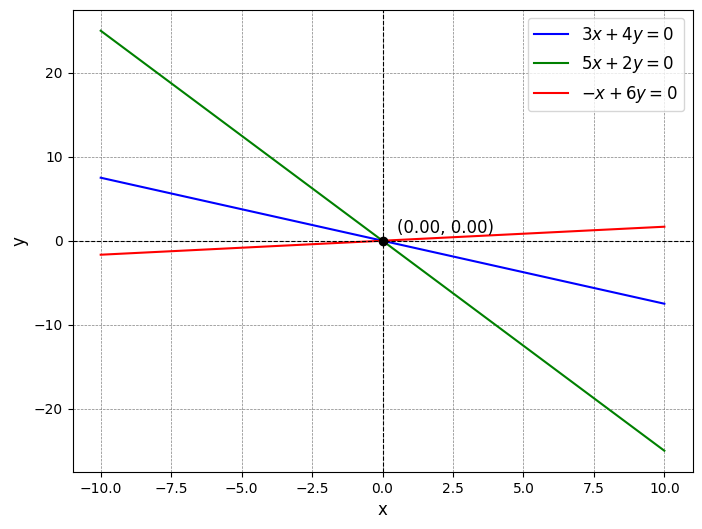
\includegraphics[scale=0.4]{images/img01}\quad  		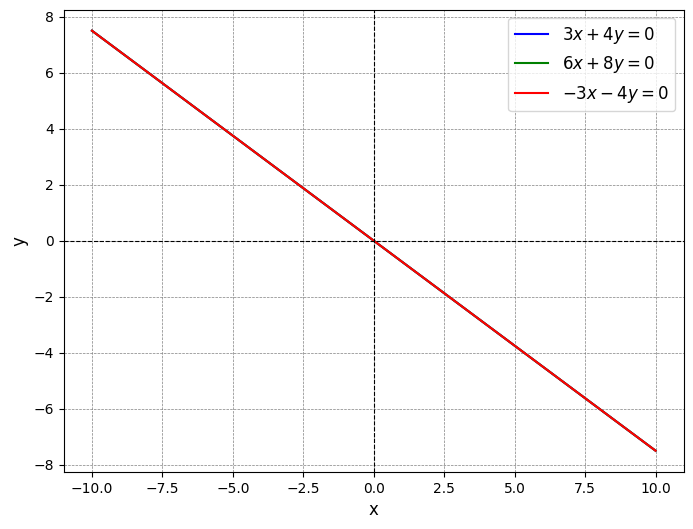
\includegraphics[scale=0.4]{images/img02}
		$$
	\end{enumerate}
	{В линейном пространстве $L_\text{о}$ решений однородной системы $AX = 0$ существует базис, который называется \textbf{фундаментальной системой решений}.}
	\\\\
	{Если столбец $B\ne 0$, то система линейных уравнений \eqref{eq:slae-1} называется \textbf{неоднородной}.}
	\\\\
	Обозначим расширенную матрицу системы
	\begin{equation*}
		\widetilde A = \Big(A | B\Big) = \begin{pmatrix}
			a_{11} & \ldots & a_{1n} & b_1\\
			\vdots & \ddots & \vdots & \vdots \\
			a_{m1} & \ldots & a_{mn} & b_{m}
		\end{pmatrix}
	\end{equation*}
	\begin{theorem}
		[Кронекера-Капелли]
		Система линейных уравнений $AX = B$ совместна (то есть имеет хотя бы одно решение) тогда и только тогда, когда $\rank (A) = \rank (\widetilde{A})$.
	\end{theorem}
	\noindent
	{Однородная система линейных уравнений $AX = 0$ с той же матрицей $A$, что и система $AX = B$, называется \textbf{приведенной} для неоднородной системы $AX = B$.}
	\begin{theorem}
		Если $X = (x_1,\dots,x_n) \in P^n$ --- решение системы $AX = B$, а $L_\text{o}$ --- это пространство решений приведенной системы $AX = 0$, то множество решений системы $AX = B$ совпадает с множеством \begin{equation}
			L_\text{н} = \{x\} + L_\text{o} = \{ x + y \ | \ y\in L_\text{o} \}.
		\end{equation}
	\end{theorem}
	\begin{theorem}
		Система линейных уравнений $AX = B$ имеет единственное решение тогда и только тогда, когда $\rank(A) = \rank(\widetilde A) = n$.
	\end{theorem}
	\noindent
	Рассмотрим возможные случаи для неоднородной системы $AX = B$ на плоскости $\mathbb R^2$.
	\begin{enumerate}
		\item Система имеет единственное решение ($\rank(A) = \rank(\widetilde A) = n$)
		то есть все гиперплоскости в $n$-мерном пространстве пересекаются в одной точке.
		\item Система имеет бесконечное количество решений ($\rank(A)= \rank(\widetilde A) < n$)
		то есть все гиперплоскости в $n$-мерном пространстве пересекаются по подпространству размерности $n - \rank(A)$.
		\item Система не имеет решений ($\rank(A) \ne \rank(\widetilde A)$)
		то есть все гиперплоскости $n$-мерном пространстве не имеют одной общей точки пересечения (например, они пересекаются частично или параллельны)
		$$
		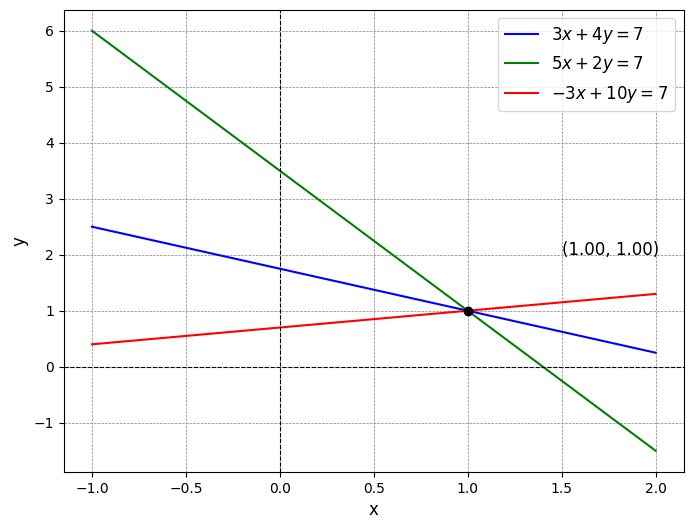
\includegraphics[scale=0.3]{images/img03} 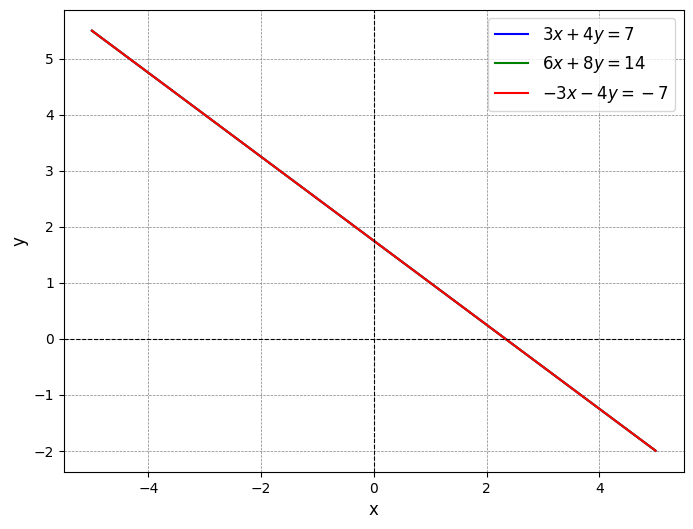
\includegraphics[scale=0.3]{images/img04}
		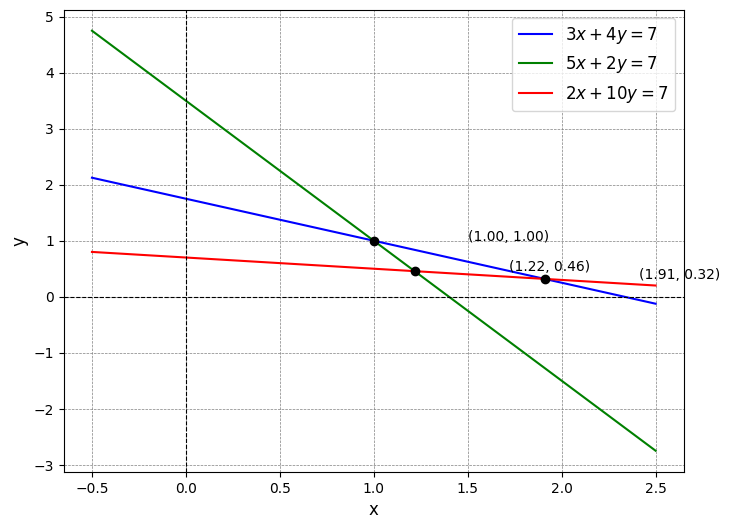
\includegraphics[scale=0.3]{images/img05}
		$$
	\end{enumerate}
	
	\chapter{Дискретная математика и алгоритмика}
	\section{Булевы функции и их представления}
	Пусть $B = \{0, 1\}$. Набор $(a_1, \dots, a_n)$, где $a_i \in \{0, 1\}$, $1 \leq i \leq n$, называется \textbf{булевым} или \textbf{двоичным набором (вектором)}. Элементы набора называют часто \textbf{компонентами} или \textbf{координатами}. Кратко набор $(a_1, \dots, a_n)$ обозначают через $\widetilde{a}^n$. 
	\textbf{Весом} (или \textbf{нормой}) набора $\widetilde{a}^n$ (обозначают $\Norm{\widetilde{a}^n}$) называют число его координат, равных 1, то есть
	\[
	\Norm{\widetilde{a}^n} = \sum_{i=1}^n a_i.
	\]
	Множество всех двоичных наборов длины $n$ образуют $n$-мерный \textbf{булев} (или \textbf{двоичный}) \textbf{куб}, который называют также единичным $n$-мерным кубом и обычно обозначают $B^n$. Наборы $\widetilde{a}^n\in B^n$ называют \textbf{вершинами} куба.
	$$
	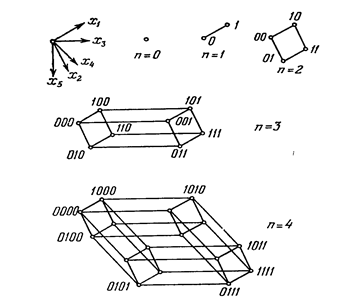
\includegraphics[scale=0.8]{images/img13}
	$$
	Функция, которая отображает $B_n$ в $B$ — \textbf{булева функция} (БФ).
	\\\\
	Если $f(x_1, x_2, \dots, x_n)$ есть БФ и $(a_1, \dots, a_n) \in B^n$, то $f(a_1, \dots, a_n)$ есть значение этой функции на наборе $(a_1, \dots, a_n)$; $f(a_1, \dots, a_n) \in B$ в случае определенности этого значения (возможно, что $f(a_1, \dots, a_n)$ не определено).
	Пусть $\widetilde{x}^n = (x_1, x_2, \dots, x_n)$, $n \geq 2$.
	\\\\
	Каждую БФ $f(\widetilde{x}^n)$ можно задать следующей \textbf{таблицей}, в которой в первых $n$ столбцах перечислены все наборы значений $n$ аргументов в так называемом естественном порядке, а в $(n+1)$-м столбце — значения функции.
	\[
	\begin{array}{|c|c|c|c|c|c|}
		\hline
		x_1 & \dots & x_{n-2} & x_{n-1} & x_n & f(\widetilde{x}^n) \\
		\hline
		0   & \dots & 0       & 0       & 0   & a_1 \\
		0   & \dots & 0       & 0       & 1   & a_2 \\
		0   & \dots & 0       & 1       & 0   & a_3 \\
		\vdots & \ddots & \vdots & \vdots & \vdots & \vdots \\
		1   & \dots & 1       & 1       & 1   & a_{2^n} \\
		\hline
	\end{array}
	\]
	БФ $f(\vec{x}^n)$ можно определить \textbf{векторным заданием}
	\[
	f(\widetilde{x}^n) = (a_1, a_2, \dots, a_{2^n}),
	\]
	где набор $(a_1, a_2, \dots,a_{2^n-1}, a_{2^n})$ есть столбец значений БФ из ее табличного задания, поскольку наборы значений аргументов легко восстановить.
	\begin{theorem}
		[о числе различных БФ от $n$ аргументов] Число всех различных БФ от $n$ аргументов равно $2^{2^n}$.
	\end{theorem}
	\noindent
	Переменные бывают существенные и фиктивные. Переменная $x_i$ \textbf{существенна}, если существует такой набор $(a_1,\ldots, a_{i-1}, a_{i+1},\ldots, a_n)$ значений аргументов $(x_1,\ldots, x_{i-1}, x_{i+1},\ldots, x_n)$, что	
	\[
	f(x_1, \dots, x_{i-1}, 0, x_{i+1}, \dots, x_n) \neq f(x_1, \dots, x_{i-1}, 1, x_{i+1}, \dots, x_n);
	\]
	в противном случае $x_i$ \textbf{фиктивна}.
	\\\\
	В таблице ниже перечислены БФ, которые называются \textbf{элементарными}.
	\[
	\begin{array}{|c|c|c|c|c|c|c|c|c|}
		\hline
		x & y & x \land y & x \lor y & x \to y & x \leftrightarrow y & x \oplus y & x \uparrow y & x \downarrow y \\
		\hline
		0 & 0 & 0 & 0 & 1 & 1 & 0 & 1 & 1 \\
		0 & 1 & 0 & 1 & 1 & 0 & 1 & 1 & 0 \\
		1 & 0 & 0 & 1 & 0 & 0 & 1 & 1 & 0 \\
		1 & 1 & 1 & 1 & 1 & 1 & 0 & 0 & 0 \\
		\hline
	\end{array}
	\]
	Элементарные булевы функции:
	\begin{itemize}
		\item Конъюнкция ($\land$),
		\item Дизъюнкция ($\lor$),
		\item Импликация ($\to$),
		\item Эквиваленция ($\leftrightarrow$),
		\item Сумма по модулю 2 ($\oplus$),
		\item Штрих Шеффера ($\uparrow$),
		\item Стрелка Пирса ($\downarrow$).
	\end{itemize}
	Пусть задано некоторое множество $F$ БФ, причем $F \neq 0$. Например, множество всех элементарных БФ обозначим через $F_0$, и имеем $F_0 \neq 0$.
	\\\\
	Индуктивное определение формулы под множеством $F$ БФ:
	\begin{enumerate}
		\item Каждая функция $f(x^n)$ из $F$ называется \textbf{формулой} над $F$.
		\item Пусть $f(x_1, \dots, x_n) \in F$, а $A_1, \dots, A_n$ — формулы над $F$.
	\end{enumerate}
	Тогда выражение $f(A_1, \dots, A_n)$ называется \textbf{формулой} над $F$.
	\begin{theorem}[о дизъюнктивном разложении БФ]
		Для каждой БФ $f(x^n)$ и любого $k$ $(1 \leq k \leq n)$ справедливо равенство
		\[
		f(a_1, \dots, a_n) = \bigvee_{(a_1, \dots, a_k)} x_1^{a_1}\cdot \ldots \cdot x_k^{a_k}\cdot f(a_1,\ldots, a_k,x_{k+1},\ldots, x_n),
		\]
		где дизъюнкция берется по всем $k$-наборам из $0$ и $1$.
	\end{theorem}
	Для любой БФ $f(\widetilde{x}^n)$ справедливы равенства:
	\begin{equation}
		f(\widetilde{x}^n) = x_n \cdot f(\widetilde{x}^{n-1}, 1) \lor \overline{x_n} \cdot f(\widetilde{x}^{n-1}, 0),
	\end{equation}
	\begin{equation}
		\label{bf-1}
		f(\widetilde{x}^n) = \bigvee_{(a_1, \dots, a_n)} x_1^{a_1} \cdots x_n^{a_n} \cdot f(a_1, \dots, a_n). 
	\end{equation}
	Если же $f(\widetilde{x}^n) \neq 0$, то из равенства \eqref{bf-1} вытекает:
	\begin{equation}
		\label{bf-2}
		f(\widetilde{x}^n) = \bigvee_{(a_1, \dots, a_n) \,:\, f(a_1, \dots, a_n) = 1} x_1^{a_1} \cdot x_2^{a_2} \cdots x_n^{a_n}.
	\end{equation}
	Правая часть равенства \eqref{bf-2} называется \textbf{совершенной дизъюнктивной нормальной формой (СДНФ)} функции $f(\widetilde{x}^n)$.
	Ее можно привести к виду
	\begin{equation}
		\label{bf-3}
		f(\widetilde{x}^n) = \bigwedge_{(a_1, \dots, a_n) \,:\, f(a_1, \dots, a_n) = 0} (x_1^{\overline a_1} \vee x_2^{\overline a_2} \vee \ldots \vee  x_n^{\overline a_n}).
	\end{equation}
	Правая часть равенства \eqref{bf-3} называется \textbf{совершенной конъюнктивной нормальной формой (СКНФ)} функции $f(\widetilde{x}^n)$.
	\\\\
	Выражение вида $K_1\oplus \ldots \oplus K_s$, где $K_i = 1,\ldots, s$ -- попарно различные элементарные конъюнкции, не содержащие отрицаний переменных, над множеством переменных $\{x_1,\ldots, x_n\}$ ранга от $0$ до $n$, называется \textbf{полиномом по модулю два} или \textbf{полиномом Жегалкина}
	\begin{equation}
		f(\widetilde{x}^n)=a_0\oplus a_1x_1 \oplus a_2 x_2\oplus \ldots\oplus a_{12}x_1x_2\oplus \ldots \oplus a_{123}x_1 x_2 x_3 \oplus \ldots.
	\end{equation}
	\begin{theorem}
		[Жегалкина] Каждая БФ единственным образом представим в виде полинома Жегалкина.
	\end{theorem}
	\noindent
	Одним из алгоритмов построения полиномов mod 2 является
	следующий. Для БФ $f(\widetilde{x}^n)$ находят ее СДНФ, затем в этой формуле всюду заменяю $\vee$ на $\oplus$, $\overline x_i$ на $x_i\oplus 1$ и используют равенство $x(y\oplus z)=xy\oplus xz$ требуемое число раз.
	\\\\
	Система $M$ называется \textbf{полной}, если любую БФ можно представить формулой над $M$
	\begin{theorem}
		Система $\{\neg, \vee, \wedge\}$ является полной.
	\end{theorem}
	\begin{theorem}
		Система $\{\neg, \oplus, 1\}$ является полной.
	\end{theorem}
	\noindent
	\textbf{Замыканием} множества $M$
	называется множество $[M]$, состоящее из всех БФ,
	которые могут быть заданы формулой над $M$. Класс $M$ БФ называется
	\textbf{замкнутым}, если $[M]=M$.
	\\\\
	\textbf{Важнейшие замкнутые классы БФ}:
	\begin{enumerate}
		\item $T_0 = \{f \in P_2 \mid f(0, 0, \ldots, 0) = 0\}$~--- множество БФ, которые сохраняют константу 0.
		\item $T_1 = \{f \in P_2 \mid f(1, 1, \ldots, 1) = 1\}$~--- множество БФ, которые сохраняют константу 1.
		\item $S = \{f \mid f(\widetilde{x}^n) = f(\bar{x}_1, \ldots, \bar{x}_n)\}$~--- самодвойственные.
		\item $L = \{\text{Если } \exists a_0, \ldots, a_n: f(\widetilde{x}^n) = a_0 \oplus a_1 x_1 \oplus \ldots \oplus a_n x_n\}$~--- линейные.
		\item $M = \{f(a_1, \ldots, a_n) < f(b_1, \ldots, b_n) \text{ при } (a_1, \ldots, a_n) < (b_1, \ldots, b_n)\}$~--- монотонные.
	\end{enumerate}
	\begin{theorem}
		[критерий полноты]
		Для того чтобы система $A$ была \textit{полной}, необходимо и достаточно, чтобы была хотя бы одна функция $f$ из системы $A$, которая не принадлежит ни одной из систем $T_0, T_1, L, S, M$.
	\end{theorem}
	\section{Основные классы графов}
	\textbf{Граф} -- это упорядоченная пара множеств $G = (V,E)$ множеств $V$ и $E$ при условии, что $V \ne 0$, $E \subseteq [V]^2$. Таким образом, элементами множества $E$ являются двухэлементные подмножества множества $V$. Такие графы называются \textbf{неориентированными}. Элементы множества $V$ называются \textbf{вершинами}, а множества $E$ -- \textbf{ребрами}.
	\\\\
	Рассмотрим основные способы задания графов.
	\begin{enumerate}
		\item Отношение изоморфизма графов – отношение эквивалентности
		(симметрично, транзитивно, рефлексивно). Изоморфные графы
		отождествляют. -- с помощью явного указания множества вершин $V$ и множества ребер $E$.
		$$
			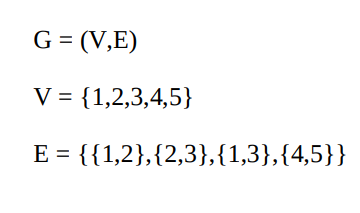
\includegraphics[scale=0.5]{images/img29}
		$$
		\item Обычно графы изображают, рисуя каждую вершину как точку на
		плоскости (в пространстве), и соединяют две точки линией, если
		соответствующие им вершины соединены ребром. Линии соединений не
		должны образовывать новых вершин. Такие изображения графа называются
		его \textbf{геометрической реализацией}.
		$$
			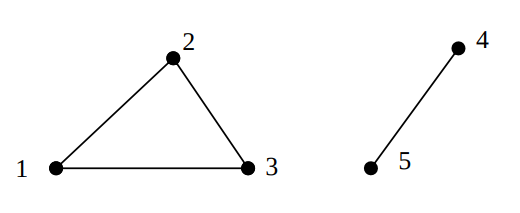
\includegraphics[scale=0.5]{images/img28}
		$$
		\item Пусть \( G \) --- помеченный граф порядка \( n \):$
		V(G)=\{1,2,3,\ldots,n\}.$
		Определим бинарную матрицу \( n \times n \) : $A = A(G)$,
		заданную следующим образом:
		\[
		A_{i,j} = \begin{cases}
			1, & \text{если вершины \(i\) и \(j\) смежные},\\[1mm]
			0, & \text{если вершины \(i\) и \(j\) не смежные}.
		\end{cases}
		\]
		\( A \) --- \textbf{матрица смежности графа} \( G \).
		\begin{equation*}
			A = \begin{pmatrix}
				1 & 1 & 1 & 0 & 0\\
				1 & 1 & 1& 0 & 0\\
				1 & 1 & 1& 0 & 0\\
				0 & 0 & 0 & 1 & 1 \\
				0 & 0 & 0 & 1 & 1
			\end{pmatrix}
		\end{equation*}
		\item \textbf{Матрица Кирхгофа}Определим матрицу \(B = \bigl(B_{i,j}\bigr)\) следующим образом:
		\[
		B_{i,j} = 
		\begin{cases}
			-1, & \text{если вершины } i,j \text{ смежны},\\[1mm]
			0,  & \text{если } i \neq j \text{ и вершины } i,j \text{ несмежны},\\[1mm]
			\deg\, i, & \text{если } i = j.
		\end{cases}
		\]
		\begin{equation*}
			B = \begin{pmatrix}
				2 & -1 & -1 & 0 & 0\\
				-1 & 2 & -1& 0 & 0\\
				-1 & -1 & 2& 0 & 0\\
				0 & 0 & 0 & 1 & -1 \\
				0 & 0 & 0 & -1 & 1
			\end{pmatrix}
		\end{equation*}
		Сумма элементов в каждой строке и в каждом столбце этой матрицы равна 0.
		Алгебраические дополнения всех элементов матрицы Кирхгофа равны между собой.
		\item Пусть граф \( G \) имеет \( n \) вершин
		$
		V(G) = \{1, 2, \dots, n\},
		$
		и \( m \) рёбер
		$
		E(G) = \{l_1, l_2, \dots, l_m\}.
		$
		\textbf{Инцидентная матрица} графа \( G \) – это бинарная матрица размера \( n \times m \), задающаяся следующим образом:
		\[
		I_{k,l} = \begin{cases}
			1, & \text{если вершина } k \text{ и ребро } l \text{ инцидентны,} \\
			0, & \text{иначе.}
		\end{cases}
		\]
		Отметим, что в каждом столбце матрицы ровно две единицы, и никакие два столбца не совпадают.
		\begin{equation*}
			I = \begin{pmatrix}
				1 & 0 & 1 & 0\\
				1 & 1 & 0 & 0\\
				0 & 1 & 1 & 0\\
				0 & 0 & 0 & 1\\
				0 & 0 & 0 & 1
			\end{pmatrix}
		\end{equation*}
	\end{enumerate}
	Два графа \textbf{изоморфны}, если между множествами их вершин существует
	взаимно-однозначное соответствие, сохраняющее смежность. Т.е. существует
	биекция $\varphi : V \to V$ такая, что 
	\begin{eqnarray*}
		\{x,y\} \in E \Longleftrightarrow \{\varphi(x),\varphi(y)\}\in E'\ \forall x ,y \in V.
	\end{eqnarray*}
	Содержательно изоморфизм двух графов означает, что они \textit{могут быть
	представлены одной и той же фигурой}. Отношение изоморфизма графов -- отношение эквивалентности
	(симметрично, транзитивно, рефлексивно). Изоморфные графы
	отождествляют.
	\\\\
	\textbf{Дерево} – связный граф без циклов.
	\textbf{Лес} – это граф, компонент которого являются деревьями.
	$$
		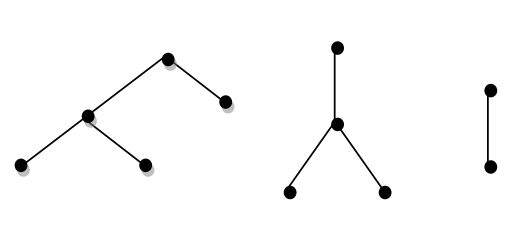
\includegraphics[scale=0.5]{images/img31}
	$$	
	Рассмотрим свойства деревьев.
	\begin{enumerate}
		\item Граф $G$ -- дерево $\Leftrightarrow$ для любых двух вершин $a$ и $b$ дерева $Т$ существует единственный путь из $a$ в $b$.
		\item Граф $G$ -- дерево $\Leftrightarrow$ если у связного графа имеется $l$ ребер и $v$ вершин, то $v = l+1$.
		\item Граф $G$ не имеет циклов; если какую-либо пару его несмежных
		вершин соединить ребром, то итоговый граф будет иметь ровно 1 цикл.
		\item Дерево не имеет кратных ребер и петель. Любое дерево – двудольный
		граф.
	\end{enumerate}
	\begin{theorem}
		[Кэли]
		Число различных деревьев, которые можно построить на $n$
		нумерованных вершинах, равно $n^{n-2}$.
	\end{theorem}
	\noindent
	Понятие дерева широко используется во многих областях математики и
	информатики. Например, они используются как инструмент при
	вычислениях, как удобный способ хранения данных (TA), способ сортировки
	или поиска данных.
	\\\\
	Граф называется \textbf{двудольным}, если существует такое разбиение множества
	его вершин на две части (доли), что концы каждого ребра принадлежат
	разным частям. Если при этом любые две вершины, входящие в разные доли,
	смежны, то граф называется \textbf{полным двудольным}.
	$$
		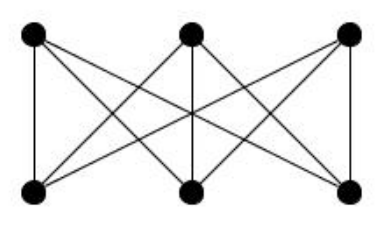
\includegraphics[scale=0.5]{images/img30}
	$$
	\begin{theorem}
		[Кенинга]
		Для двудольного графа необходимо и достаточно,
		чтобы он не содержал циклов нечётной длины.
	\end{theorem}
	\noindent
	Граф называется \textbf{планарным}, если его можно изобразить на
	плоскости так, что никакие его два ребра (за исключением ребер выходящих
	из одной вершины) не имеют общих точек. Граф, нарисованный таким
	образом, называется \textbf{плоским} графом.
	\\\\
	\textbf{Гранью} плоского графа называется максимальное множество
	точек плоскости, каждую пару которых можно соединить кривой, не
	пересекающей ребра графа. Грань, которая имеет бесконечную площадь,
	называется \textbf{внешней}, остальные грани – \textbf{внутренними}.
	\begin{theorem}
		[Эйлера]
		Если $G$ -- связный плоский граф, содержащий $n$
		вершин и $m$ ребер и $f$ граней, то $n-m+f = 2$.
	\end{theorem}
	\noindent
	Два графа \textbf{гомеоморфны}, если существует такие их
	подразделения, которые между собой изоморфны. Граф $G'$ называют \textbf{подразделением} графа $G$, если он может быть
	получен из графа $G$ путем применения некоторого числа раз операции
	подразделения ребер. \textbf{Подразделением ребра} $(а,b)$ графа $G$ называют переход от графа
	подразделением графа
	$G = (V, E)$
	к графу
	$G' = (V,E)$
	следующим образом:
	\begin{enumerate}
		\item Ребро $(а,b)$ удаляется из множества $Е$;
		\item Новая вершина $С$ добавляется во множество $V$;
		\item Новые ребра добавляются во множество $G$.
	\end{enumerate}
	\begin{theorem}
		[Критерий планарности Понтрягина-Куратовского]
		Граф $G$ планарен $\Leftrightarrow$ он не содержит подграфов гомеоморфных $K_{3,3}$, $K_{5}$
		$$
		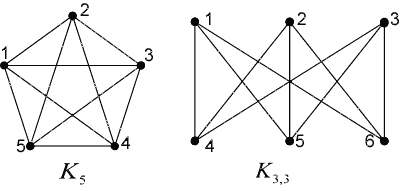
\includegraphics[scale=0.5]{images/img32}
		$$
	\end{theorem}
	\noindent
	Цикл в графе называется \textbf{эйлеровым}, если он содержит все ребра.
	\begin{theorem}
		Граф с более чем одной вершиной имеет эйлеров
		цикл тогда и только, когда он связный и каждая его
		вершина имеет чётную степень.
	\end{theorem}
	\noindent
	Связный граф с эйлеровым циклом называется \textbf{эйлеровым графом}.
	$$
		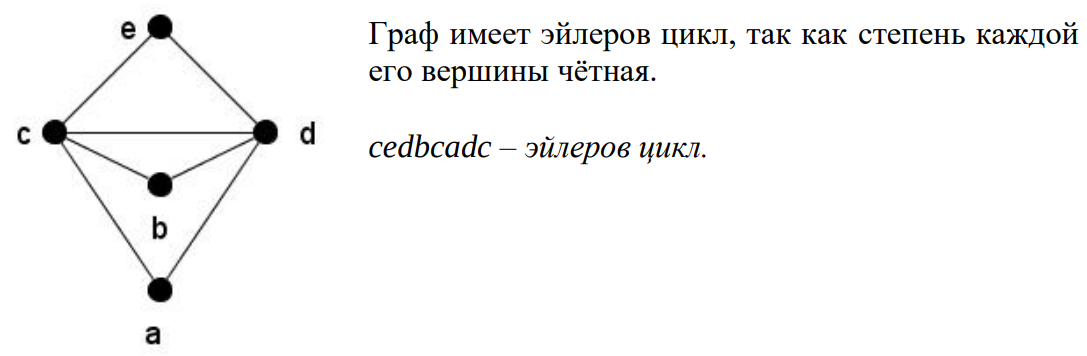
\includegraphics[scale=0.5]{images/img33}
	$$
	Если граф имеет простой цикл, содержащий все вершины графа по одному разу,
	то такой цикл называется \textbf{гамильтоновым} циклом, а граф называется \textbf{гамильтоновым}
	графом. Граф, который содержит простой путь, проходящий через каждую его вершину,
	называется \textbf{полугамильтоновым}.
	$$
		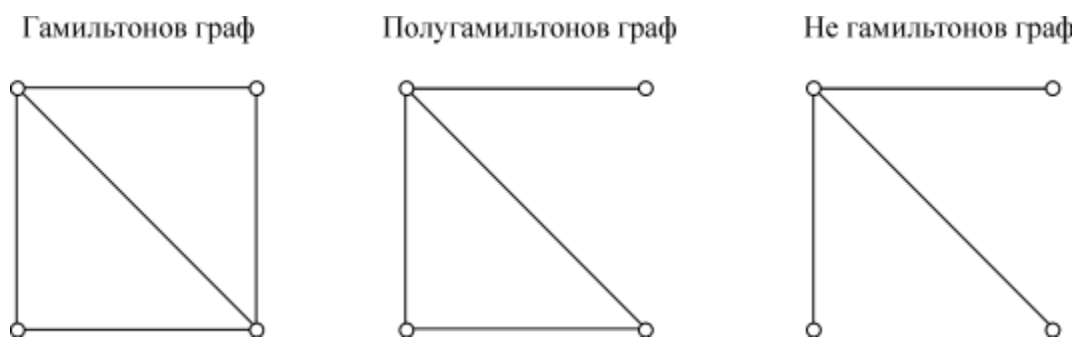
\includegraphics[scale=0.5]{images/img34}
	$$
	Гамильтонов цикл не обязательно содержит все ребра графа.
	\\\\
	Рассмотрим несколько достаточных условий существования гамильтоновых
	циклов в графе.
	\begin{enumerate}
		\item всякий полный граф является гамильтоновым. Действительно, он содержит
		такой простой цикл, которому принадлежат все вершины данного графа.
		\item если граф, помимо простого цикла, проходящего через все его вершины,
		содержит и другие ребра, то он также является гамильтоновым.
	\end{enumerate}
	\begin{theorem}
		[Дирака]
		Если в простом графе с $n > 3$ вершинами $\deg (v) > n/2$ для любой вершины $v$, то граф $G$
		является гамильтоновым. 
	\end{theorem}
	\begin{theorem}
		[Оре]
		Если число вершин графа $G(V, E)$ $n > 3$ и для любых двух несмежных вершин $u$ и
		$v$ выполняется неравенство:
		$$\deg(u) + \deg(v) > n,$$  то граф $G$ -- гамильтонов.
	\end{theorem}
	\noindent
	Теоремы не применимы к планарным графам.
	\\\\
	Пусть $G$ – граф. \textbf{Раскраской графа} $G$ называется
	окрашивание вершин графа $G$ так, что никакие две
	смежные вершины не окрашены в один цвет. Тогда
	$С_G(\lambda)$ – число способов раскраски графа $G$ в $\lambda$
	цветов так, что никакие две смежные вершины не
	окрашены в один цвет.
	\\\\
	Для фиксированного графа $G$ функция $С_G(\lambda)$ является полиномиальной
	функцией от $\lambda$ и называется \textbf{хроматическим многочленом} графа $G$.
	\textbf{Хроматическое число} графа – наименьшее число цветов, которое
	используется для раскраски графа.
	$$
		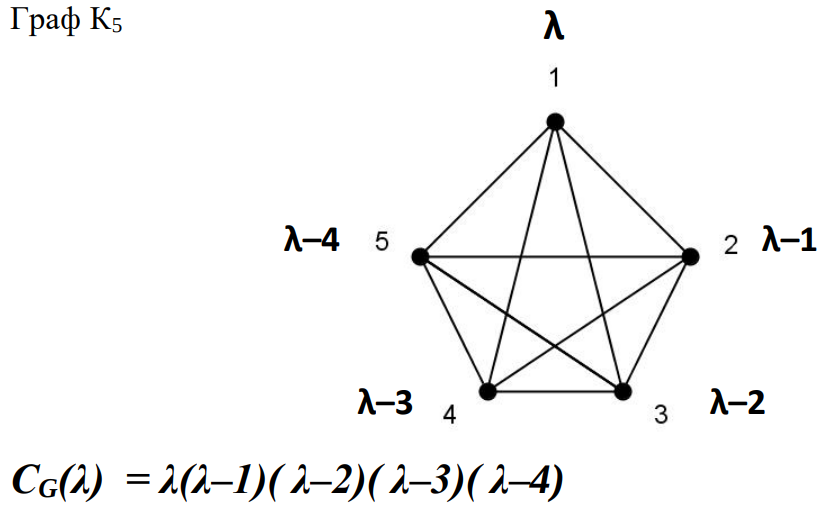
\includegraphics[scale=0.4]{images/img35}
	$$
	\section{Алгоритмы и рекурсивные функции}
	\textbf{Алгоритм} -- это строгое предписание, задающее последовательность некоторых элементарных операций, выполненных в определенном порядке для решения задач одного типа.
	\\\\
	\textbf{Детерминированная машина Тьюринга} (ДМТ) есть шестерка
	\[
	T = \langle Q, A, \delta, \Lambda, q_1, q_0 \rangle,
	\]
	где
	\begin{itemize}
		\item $Q$ -- непустое конечное множество состояний,
		\item $A$ -- непустой конечный алфавит,
		\item $\Lambda$ -- пустой символ, $\Lambda \notin A$,
		\item $\delta$ -- функция переходов, $\delta : Q \times A \to Q \times A \times \{R, L, S\}$,
		\item $q_1 \in Q$ -- начальное состояние,
		\item $q_0 \in Q$ -- конечное состояние.
	\end{itemize}
	Машина Тьюринга состоит из бесконечной ленты с записанными на ней символами из некоторого конечного алфавита и автоматического устройства -- головки чтения записей, способной считывать символы с ленты, записывать на нее новые символы и перемещаться вдоль ленты в обоих направлениях. Автоматическое устройство может находится в одном из состояний, число которых конечно.
	$$
	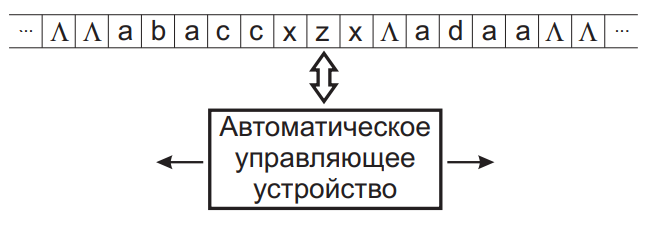
\includegraphics[scale=0.5]{images/img45}
	$$
	Начальное состояние --- $q_1$, голова считывает с ленты некоторый символ $a$.
	\textbf{Один такт работы ДМТ} в зависимости от текущего состояния:
	\begin{enumerate}
		\item Изменить состояние или оставить прежним.
		\item Записать на ленту новый символ (который может совпадать с прочитанным).
		\item Сместить голову вправо (R), влево (L) или оставить её на месте (S).
	\end{enumerate}
	\textbf{Команда ДМТ} для записи одного действия:
	\[
	qa \rightarrow q'a'd, \quad \text{где } d \in \{L, R, S\}
	\]
	или проще
	\[
	qaq'a'd,
	\]
	где $q'$ -- новое состояние машины, $a'$ -- записанный символ, $d$ -- направление движения головки.
	Список команд называется \textbf{программой} ДМТ.
	\\\\
	Обобщением одноленточной ДМТ является ДМТ, имеющая $k\geq 1$ лент, на каждой из которых имеется по одной считывающей головке. \textbf{\( k \)-ленточной детерминированной Машиной Тьюринга}, обозначается \( k \)-ДМТ, называется шестерка следующего вида
	\[
	M = \langle Q, A, \delta, \Lambda, q_1, q_0 \rangle,
	\]
	где символы \( Q, A, \Lambda, q_1 \) и \( q_0 \) определяются так же как и для однооленточных ДМТ, а функция перехода
	\[
	\delta : Q \times A^k \rightarrow Q \times (A \times \{L, R, S\})^k
	\]
	по текущему состоянию и набору текущих символов на \( k \) лентах задаёт новое состояние, новые \( k \) символов и направление движения каждой из \( k \) считывающих головок.
	\\\\
	Арифметическая функция  $T_M(n)$ называется \textbf{временной сложностью} вычисления $k$-ДМТ $M$, если получив на вход слово длины $n$ машина $M$ остановится не более чем через $T_M(n)$ шагов. Если на каком-либо слове длины $n$ машина не остановится, то для этого $n$ функция $T_M(n)$ не определена.
	\\\\
	\textbf{\(k\)-ленточной недетерминированной Машиной Тьюринга}, обозначается \(k\)-HMT, называется шестерка следующего вида
	\[
	\langle Q, A, \delta, \Lambda, q_1, q_0 \rangle,
	\]
	элементы которой определяются так же, как для однооленточных ДМТ, а функция перехода
	\[
	\delta : Q \times A^k \to 2^{Q \times (A \times \{L, S, R\})^k}
	\]
	по текущему состоянию и списку из \(k\) символов на лентах выдаёт конечное множество вариантов следующего шага.
	\\\\
	$k$-НМТ имеет \textbf{временную сложность} $T(n)$, если для произвольного входного слова длины $n$ найдется последовательность, состоящая не более чем из $T(n)$ конфигураций, переводящая машину в состояние $q_0$.
	\\\\
	Язык \(L\) распознается за \textbf{полиномиальное время}, если существует \(k\)-ДМТ \(M\) и полином \(p(n)\) такие, что
	\[
	T_M(n)=O(p(n)).
	\]
	Множество всех языков, распознаваемых некоторой $k$-ДМТ за полиномиальное время, образует \textbf{класс \(\mathcal{P}\)}.
	\\\\
	Другими словами, класс \(\mathcal{P}\) включает только те задачи распознавания, для которых существует полиномиальный алгоритм решения, независимый от их размера.
	\\\\
	Примерами полиномиально разрешимых задач являются поиск кратчайшего пути между любыми двумя вершинами графа, нахождение минимального потока в сети, перемножение матриц, все виды сортировки, различные геометрические задачи и т.\,д.
	\\\\
	Множество языков, распознаваемых некоторой $k$-НМТ за полиномиальное время, образует сложный \textbf{класс $\mathcal {NP}$}.
	\\\\
	Примерами задач, принадлежащих классу $\mathcal {NP}$ могут быть задачи поиска гамильтонова цикла в графе, определение существования целочисленного решения для системы линейных неравенств.
	\\\\
	Множество всех языков делятся на
	\begin{itemize}
		\item класс языков, для которых не существует распознающей машины Тьюринга (ни ДМТ, ни НМТ);
		\item класс языков $\mathcal P$, для которых существует $k$-ДМТ, распознающая язык за полиномиальное время;
		\item промежуточный класс -- класс языков $\mathcal {NP}$, для которых существует $k$-НМТ, распознающая язык за полиномиальное время;
	\end{itemize}
	Если класс $\mathcal P$ можно представить как класс задач, \textit{которые можно быстро решить}, то класс $\mathcal {NP}$ можно описать как класс задач, \textit{решение которых можно быстро проверить}.
	\begin{theorem}
		$\mathcal P \subseteq \mathcal {NP}$.
		$$
			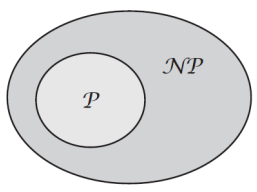
\includegraphics[scale=0.5]{images/img46}
		$$
	\end{theorem}
	\noindent
	Обратное включение $\mathcal{NP} \subseteq \mathcal P$ не доказано. Таким образом, \textbf{проблема $\mathcal P \overset{?}{=}\mathcal{NP}$} остается открытой.
	\\\\
	Задача распознавания $A$ \textbf{полиномиально сводится} к задаче распознавания $B$,
	если существует полиномиальный алгоритм, преобразующий входные данные
	задачи $A$ к таким входным данным задачи $B$, что на этих входных данных обе
	задачи имеют одинаковые решения (то есть ответ да или нет).
	\begin{theorem}
		Если задача $A$ полиномиально сводится к задаче $B$ и $B\in \mathcal P$, то $A \in \mathcal P$.
	\end{theorem}
	\noindent
	Абстрактная задача распознавания $Q$ называется \textbf{$\mathcal {NP}$-полной}, если выполняются два условия:
	\begin{enumerate}
		\item $Q \in \mathcal {NP}$;
		\item любая задача из класса $\mathcal {NP}$ полиномиально сводится к $Q$.
	\end{enumerate}
	Если выполняется только свойство 2, то задача называется \textbf{$\mathcal {NP}$-трудной.}
	\begin{theorem}
		Если хотя бы одна $\mathcal {NP}$-полная задача может быть
		решена за полиномиальное время, то
		$\mathcal P = \mathcal {NP}$. Если в классе
		$\mathcal {NP}$ существует хотя бы одна задача, неразрешимая за
		полиномиальное время, то и все $\mathcal NP$-полные задачи таковы.
		$$
			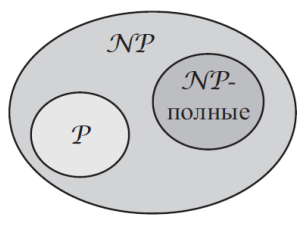
\includegraphics[scale=0.5]{images/img47}
		$$	
	\end{theorem}
	\chapter{Дифференциальные уравнения и функциональный анализ}
		\section{Линейные дифференциальные уравнения и системы}	
	\textbf{Линейным дифференциальным уравнением n-ого порядка с постоянными коэффициентами} называется уравнение вида \begin{equation}
			\label{eq:lde-n}	
			D^nx + a_{n-1}\cdot D^{n-1}x + \ldots + a_1\cdot Dx + a_0\cdot D^0x = f(t),\quad t\in \mathbb{I}\subseteq\mathbb{R},
		\end{equation} 
		где функция $f(t)$ непрерывна на промежутке (связном множестве) $\mathbb{I}$. Общее решение линейного уравнения с постоянными коэффициентами первого порядка
		\begin{equation}
			Dx - \lambda x = f(t),\ t\in\mathbb{I}\subseteq\mathbb{R}
		\end{equation} 
		можно построить в виде
		\begin{equation}
			x(t) = \int\limits e^{\lambda (t-\tau)}f(\tau)d\tau + C e^{\lambda t},\ C \in \mathbb R
		\end{equation}
	\noindent
	Построим решение для уравнения $n$-ого порядка. Обозначим через 
	\begin{equation}
		L_n = D^n + a_{n-1}D^{n-1} + \ldots + a_1D + a_0D^0
	\end{equation} 
	оператор дифференцирования. Тогда уравнение \eqref{eq:lde-n} запишем в виде 
	\begin{equation}
		L_nx=f(t),
	\end{equation}
	оператор $L_n$ является линейным.
	\noindent
	Рассмотрим линейное стационарное однородное уравнение 
	\begin{equation}
		\label{lhe}
		L_nx = 0,\ t\in \mathbb{R}.
	\end{equation}
	Множество решений линейного стационарного однородного уравнения порядка $n$ является конечномерным линейным пространством размерности $n$. А значит решение уравнения \eqref{lhe} можно представить в виде
	\begin{equation}
		x(t) = \sum_{i=1}^n C_i \phi_i(t),
	\end{equation}
	где $\phi_i(t)$ -- это базисные функции. В свою очередь базисные функции имеют следующий вид. Если $\lambda_1,\ldots,\lambda_s$ --- корни над полем $\mathbb C$ характеристического многочлена $\Delta(\lambda)$ кратности $k_1,\ldots,k_s$ соответственно, то совокупность функций $$e^{\lambda_it}, te^{\lambda_it}, t^2e^{\lambda_it},\ldots,t^{k_i-1}e^{\lambda_it},\ i=\overline{1,s}$$ является системой линейно независимых решений уравнения \eqref{lhe}. Причем комплексные решения вида $t^m e^{(\alpha+\beta i)t}$ заменяются парой двух вещественных решений $t^m e^{\alpha t}\cos \beta t$, $t^m e^{\alpha t}\sin \beta t$. Таким образом, алгоритм построения решения однородного линейного уравнения \eqref{lhe} следующий:
	Рассмотрим линейное неоднородное уравнение 
	\begin{equation}
		\label{le}
		L_nx = f(t),\ t\in \mathbb{I}
	\end{equation} и соответствующее ему линейное однородное уравнение $L_nx = 0.$ Все решения неоднородного линейного уравнения можно представить в виде $$x_{\text{он}}(t) =\phi_0(t) + \sum_{i=1}^n C_i \phi_i(t),$$
	где $\phi_0(t)$ -- это частное решение неоднородного уравнения. Частное решение строится одним из следующих способов.
	\begin{enumerate}
		\item \textbf{Метод Коши}.
		Пусть функция $f(t)$ непрерывна на $\mathbb I$ и пусть $\varphi_{n-1}(t)$ --- функция Коши (последняя функция фундаментальной системы решений нормированной при $t=0$) оператора $L_n$. Тогда функция $$\phi_0(t) = \int\limits_{t_0}^{t}\varphi_{n-1}(t-\uptau) f(\uptau)d\uptau,\ \forall t_0 \in \mathbb I.$$
		\item \textbf{Метод Лагранжа (вариации произвольной постоянной)}.
		Пусть $\varphi_1(t),\ldots,\varphi_n(t)$ --- фундаментальная система решений уравнения \eqref{lhe}. Тогда функция $$\phi_0(t) = u_1(t)\varphi_1(t) + \ldots + u_n(t)\varphi_n(t)$$ является решением уравнения \eqref{le}, если функции $u_i(t)$ удовлетворяют системе $$\begin{cases}
			Du_1\varphi_1 + \ldots + Du_n\varphi_n = 0,\\
			Du_1D\varphi_1 + \ldots + Du_nD\varphi_n = 0,\\
			\dotfill\\
			Du_1D^{n-2}\varphi_1 + \ldots + Du_nD^{n-2}\varphi_n = 0,\\
			Du_1D^{n-1}\varphi_1 + \ldots + Du_nD^{n-1}\varphi_n = f(t).
		\end{cases}$$
		\item \textbf{Метод Эйлера}. Уравнение $$L_nx = P(t)\cdot e^{\upgamma t},$$ где $x(t)$ --- неизвестная действительная функция, $P(t)\in\mathbb R[t]$, $\deg P(t) = m$, $\upgamma \in \mathbb R$, имеет частное решение вида $$\phi_0(t) = t^k\cdot Q(t)\cdot e^{\upgamma t},$$ где $Q(t) \in \mathbb R[t], \deg Q(t) \leqslant m$, $k$ --- кратность корня $\upgamma$ характеристического многочлена $\Delta(\lambda)$.
	\end{enumerate}
	\textbf{Системой линейных дифференциальных уравнений первого порядка с постоянными коэффициентами} называется система вида
	$$\begin{cases}
		Dx_1=a_{11}\cdot x_1(t) + \ldots + a_{1n}\cdot x_n(t) + f_1(t),\\
		\dotfill\\
		Dx_n=a_{n1}\cdot x_1(t) + \ldots + a_{nn}\cdot x_n(t) + f_n(t);
	\end{cases}\quad t \in \mathbb I.$$ Любую систему $k$ дифференциальных уравнений произвольного порядков $m_1,\ldots, m_k$ можно привести к системе $m_1+\ldots + m_k$ уравнений первого порядка. В матричном виде можно записать систему как
	\begin{equation}
		\label{lsys}
		Dx = Ax + f(t),
	\end{equation}
	где $x(t)$, $f(t)$ -- это $n$-мерные векторы, а $A=(a_{ij})$ -- это $n\times n$ матрица. Все методы отыскания решений линейных уравнений обобщаются до систем.
	\\\\
	Рассмотрим однородную систему 
	\begin{equation}
		\label{hsys}
		Dx = Ax.
	\end{equation}
	\begin{theorem}[Метод Эйлера]
		Если $B_0, B_1, \ldots, B_k$ --- жорданова цепочка матрицы $A$, соответствующая собственному значению $\lambda_0$, то векторная функция $$x(t) = \Big(B_0\dfrac{t^k}{k!} + B_1\dfrac{t^{k-1}}{(k-1)!} + B_2\dfrac{t^{k-2}}{(k-2)!} + \ldots + B_{k-1}\dfrac{t}{1!} + B_k\Big)\cdot e^{\lambda_0 t}$$ является решением уравнения \eqref{hsys}. 
	\end{theorem}
	\noindent
	Решение системы \eqref{hsys} можно также построить в виде матричной экспоненты
	\begin{equation}
		x(t) = e^{At}C,
	\end{equation}
	где $e^{At}$ -- матрица, $C$ -- $n$-мерный вектор произвольных постоянных.
	\\\\
	Для построения частного решения неоднородного уравнения \eqref{lsys} можно воспользоваться одним из следующих методов.
	\begin{enumerate}
		\item \textbf{Метод Лагранжа}. Представляем частное решение в виде
		\begin{equation}
			x_0(t) = x_1(t)\cdot u_1(t) + \ldots + x_n(t)\cdot u_n(t),
		\end{equation}
		где $[x_1(t),\ldots, x_n(t)]$ -- это матрица фундаментальных решений однородной системы \eqref{hsys}, а $u_1(t),\ldots, u_n(t)$ -- это произвольные функции, которые подлежат определению путем подстановки в уравнение \eqref{lsys}.
		\item \textbf{Метод Коши.} Частное решение имеет вид
		\begin{equation}
			x_0(t) = \int\limits_{t_0}^t e^{A(t-\tau)}f(\tau)d\tau.
		\end{equation}
	\end{enumerate}
	Тогда, например, если использовать матричную экспоненту для представления общего решения, получим решение неоднородной системы \eqref{lsys} в виде
	\begin{equation}
		x_{\text{он}}(t) =e^{At} C + \int\limits_{t_0}^t e^{A(t-\tau)}f(\tau)d\tau.
	\end{equation}
	В общем случае, если рассматривать систему нестационарных линейных уравнений вида
	\begin{equation}
		Dx = A(t)\cdot x(t) + f(t),\ t \in \mathbb I.
	\end{equation}
	Пусть $\Phi(t)$ -- это матрица фундаментальных решений однородной линейной системы $Dx = A(t)\cdot x(t)$. Тогда по \textbf{формуле Коши} можно записать решение неоднородной системы
	\begin{equation}
		x_{\text{он}}(t) =\Phi(t) C + \int\limits_{t_0}^t \Phi(t) \Phi^{-1}(\tau)f(\tau)d\tau.
	\end{equation}
	\section{Общая теория дифференциальных уравнений}
	Рассмотрим задачу Коши 
	\begin{equation}
		\label{eq:cauchi-1}
		\begin{cases}
			y' = f(x,y),\ (x,y)\in D\subseteq \mathbb R^2,\\
			y(x_0) = y_0,\ (x_0,y_0)\in D;
		\end{cases}
	\end{equation}
	где $f(x,y)$ --- непрерывная в некоторой области $D$ функция.\\\\
	Важным является вопрос о корректности поставленной задачи. Задача Коши называется \textbf{корректно поставленной}, если
	\begin{enumerate}
		\item для любых входных данных решение задачи существует;
		\item для любых входных данных решение задачи единственно;
		\item решение устойчиво по входным данным.
	\end{enumerate}
	На вопрос существования и единственности решения задачи Коши отвечает теорема Пикара-Линделефа.
	\begin{theorem}
		[Пикара-Линделефа]
		Если функция $f(x,y)$ непрерывна в некоторой области $D\subseteq\mathbb R^2$ и в некоторой окрестности $U$ содержащейся в $D$ удовлетворяет условию Липшица по $y$, то есть $$\exists L:\forall (x,y_1),(x,y_2)\in U\quad |f(x,y_1) - f(x,y_2)| \leq L|y_1 - y_2|,$$
		то задача Коши \eqref{eq:cauchi-1} имеет единственное решение.
	\end{theorem}
	\begin{theorem}
		[об условии Липшица]
		Если на некотором замкнутом ограниченном множестве $U\subseteq \mathbb R^2$ функция $f(x,y)$ непрерывна вместе со своей частной производной $f'_y$, то функция $f(x,y)$ удовлетворяет условию Липшица по $y$.
	\end{theorem}
	\noindent
	Таким образом, при определенных условиях на функцию $f$ задача Коши \eqref{eq:cauchi-1} для дифференциального уравнения первого порядка однозначно разрешима.
	Теперь обобщим это до случая дифференциального уравнения $n$-ого порядка.
	\\\\
	Задача Коши для уравнения $n$-ого порядка имеет вид 
	\begin{equation}
		\label{eq:cauchi-2}
		\begin{cases}
			y^{(n)} = f(x, y, y', \ldots, y^{(n-1)}),\\
			y(x_0) = y_0,\ y'(x_0) = \xi_1,\ \ldots,\ y^{(n-1)}(x_0) = \xi_{n-1}.
		\end{cases}
	\end{equation}
	Задачу Коши \eqref{eq:cauchi-2} можно свести к системе $n$ уравнений первого порядка. 
	Рассмотрим произвольную систему $k$ дифференциальных уравнений порядков $m_1,\ldots, m_k$.
	Система дифференциальных уравнений \textbf{имеет нормальную форму}, если она состоит из уравнений вида $$D^{m_i}x_i(t) = f_i(t,x_1(t),Dx_1,\ldots,D^{m_1-1}x_1, \ldots, x_k(t), Dx_k, \ldots, D^{m_k - 1}x_k),\quad i = 1,\ldots, k.$$
	Эту систему можно заменить эквивалентной ей системой из $m_1+\ldots +m_k$ уравнений первого порядка.\\\\
	Следовательно, далее рассматриваем задачу Коши для системы $n$ дифференциальных уравнений первого порядка
	\begin{equation}
		\label{ode-sys}
		\begin{cases}
			\dfrac{dx_1}{dt} = f_1(t, x_1(t),\ldots, x_n(t)),\\
			\dotfill\\
			\dfrac{dx_n}{dt} = f_n(t, x_1(t),\ldots, x_n(t)),\\
			x_1(t_0) =  \xi_1,\ldots, x_n(t_0)=\xi_n
		\end{cases}
	\end{equation}
	или в векторной форме
	\begin{equation}
		\label{cauchi-3}
		\begin{cases}
			\dfrac{d\mathbf x}{dt} = \mathbf f(t,\mathbf x(t)),\\
		\mathbf x(t_0) = \mathbf \xi,
		\end{cases}
	\end{equation}
	где $t_0$ из некоторого промежутка $\mathbb I$.
	Для системы $n$ дифференциальных уравнений первого порядка справедлива следующая теорема.
	\begin{theorem}
		Если функции $f_i(t, x_1, \ldots, x_n)$ $\forall i = \overline{1,n}$ непрерывны по всем своим аргументам в области $D$ и удовлетворяют условию Липшица по каждой переменной $x_i$ в окрестности некоторой точки $(t_0, \xi_1,\ldots, \xi_n)$, то задача Коши $$\begin{cases}
			x'_i = f_i(t, x_1, \ldots, x_n),\\
			x_i (t_0) = \xi_i;
		\end{cases}$$ имеет единственное решение в окрестности этой точки.
	\end{theorem}
	\noindent
	Пусть $\mathbf x_0(t)$ -- это решение задачи Коши \eqref{cauchi-3}. Тогда решение $\mathbf x_0$ называется \textbf{непрерывно зависящим от начальных данных} на промежутке  $\mathbb I$, если
	\begin{equation}
		\forall \epsilon > 0,\ \exists \delta > 0 : \forall \mathbf x(t),\ \Norm{\mathbf x(t_0) - \mathbf x_0(t_0)} < \delta \Rightarrow \Norm{\mathbf x(t) - \mathbf x_0(t)} < \epsilon\ \forall t \in \mathbb I.
	\end{equation}
	Под этим понимается, что при малом изменении начальных данных в задаче, решения задач Коши должны слабо отклоняться друг от друга:
	
	$$
	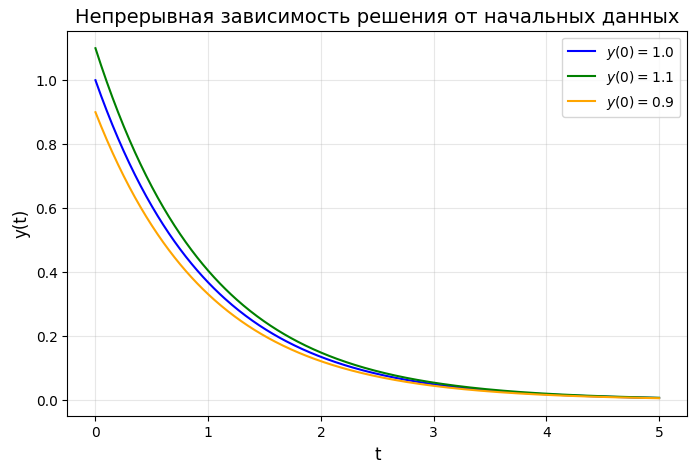
\includegraphics[scale=0.4]{images/img21}\
	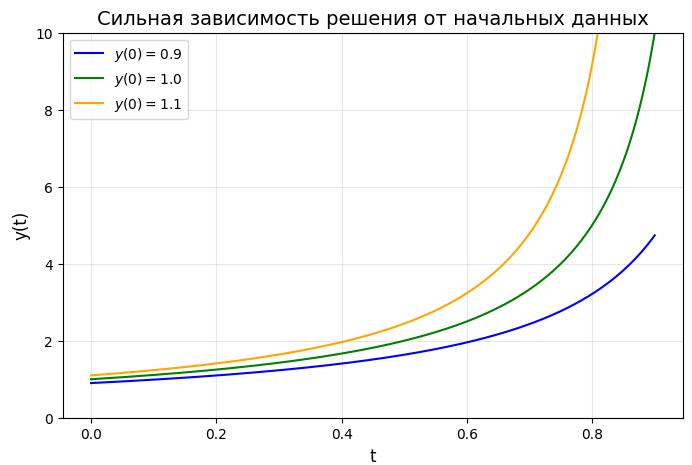
\includegraphics[scale=0.4]{images/img22}
	$$
	Пусть $\mathbf f_0(t,\mathbf x(t))$ -- это конкретная правая часть, при которой получается решение $\mathbf x_0(t)$ в задаче Коши. Тогда решение $\mathbf x_0$ называется \textbf{непрерывно зависящим от правой части} на промежутке $\mathbb I$, если
	\begin{equation}
		\forall \epsilon > 0,\ \exists \delta > 0 : \forall \mathbf x(t) \text{ с } \mathbf f,\ \underset{t}{\sup}|\mathbf f(t, \mathbf x(t)) - \mathbf f_0(t, \mathbf x(t))|<\delta \Rightarrow \Norm{\mathbf x(t) - \mathbf x_0(t)} < \epsilon\ \forall t \in \mathbb I.
	\end{equation}
	Под этим понимается, что при малом изменении правой части в задаче, решения задач Коши должны слабо отклоняться друг от друга:
	$$
	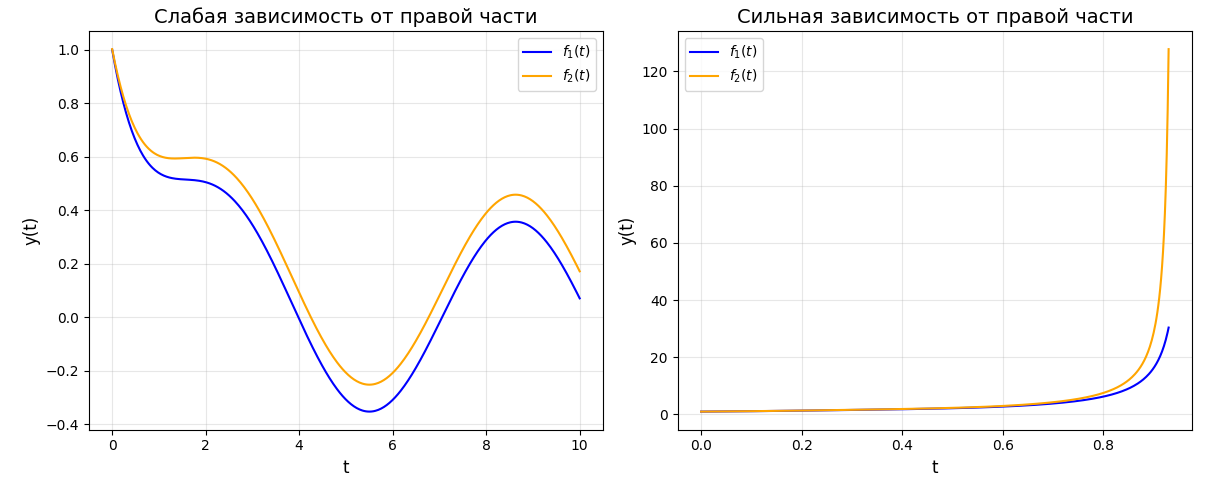
\includegraphics[scale=0.5]{images/img23}
	$$
	Если функция $\mathbf f$ в задаче \eqref{cauchi-3} является липшицевой, что равносильно тому, что она имеет непрерывные производные по $\mathbf x$, то можно доказать неравенство
	\begin{equation}
		\Norm{\mathbf x(t) - \mathbf x_0(t)} \leq M_1\cdot \Norm{\mathbf x(t_0) - \mathbf x_0(t)} + M_2\cdot \underset{t}{\sup}|\mathbf f(t, \mathbf x(t)) - \mathbf f_0(t, \mathbf x(t))|
	\end{equation}
	для любого решения $\mathbf x(t)$ задачи Коши с правой частью $\mathbf f$, где $M_1, M_2>0$ -- некоторые постоянные.
	Таким образом, решение задачи Коши \eqref{cauchi-3} непрерывно зависит от начальных данных и правой части, если функция $\mathbf f$ является липшицевой. Также это неравенство дает понять, что все решения системы  будут одновременно зависеть или не зависеть от начальных данных и правых частей.
	\\\\
	Решение $\mathbf x_0(t)$ задачи \eqref{cauchi-3} называется \textbf{устойчивым по Ляпунову}, если оно непрерывно зависит от начальных данных на промежутке вида $\mathbb I = [t_0; +\infty)$, то есть
	\begin{equation}
		\forall \epsilon > 0,\ \exists \delta > 0 : \forall \mathbf x(t),\ \Norm{\mathbf x(t_0) - \mathbf x_0(t_0)} < \delta \Rightarrow \Norm{\mathbf x(t) - \mathbf x_0(t)} < \epsilon\ \forall t >t_0.
	\end{equation}
	Если кроме того
	\begin{equation*}
		\lim\limits_{t \to +\infty} \Norm{\mathbf x(t) - \mathbf x_0(t)}=0,
	\end{equation*}
	то решение называется \textbf{ассимптотически устойчивым}. 
	\\\\
	Система называется \textbf{приведенной}, если 
	\begin{equation*}
		f(0,t) \equiv 0,
	\end{equation*}
	она всегда имеет нулевое решение $\mathbf x \equiv 0$. Любую систему вида \eqref{cauchi-3} можно свести к \textbf{приведенному} виду. Решение $\mathbf x_0(t)$ переходит в нулевое решение. Таким образом, в дальнейшем можно исследовать устойчивость нулевого решения приведенной системы
	\\\\
	Нулевое решение приведенной системы называется \textbf{устойчивым по Ляпунову}, если 
	\begin{equation}
		\forall \epsilon > 0,\ \exists \delta > 0 : \forall \mathbf x(t),\ \Norm{\mathbf x(t_0)} < \delta \Rightarrow \Norm{\mathbf x(t)} < \epsilon\ \forall t >t_0.
	\end{equation}
	\begin{theorem}
		[Ляпунова об устойчивости нулевого решения приведенной системы]
		Если существует функция $v : \mathbb R^n \rightarrow \mathbb R$ положительно определенная в некоторой окрестности $u$ точки $O = (0,\ldots, 0)$ и при этом 
		$$\dfrac{\d v}{\d x_1}\cdot f_1(t, x_1,\ldots, x_n) +\ldots + \dfrac{\d v}{\d x_n}\cdot f_n(t, x_1,\ldots, x_n) \leq 0\quad \forall x \in u, t > t_0,\eqno (6.4.2)$$
		то нулевое решение системы \eqref{cauchi-3} устойчиво.\\\\
		Если кроме того существует положительно определенная в окрестности $u$ функция $w : \mathbb R^n \rightarrow \mathbb R$ такая, что $$\dfrac{\d v}{\d x_1}\cdot f_1(t, x_1,\ldots, x_n) +\ldots + \dfrac{\d v}{\d x_n}\cdot f_n(t, x_1,\ldots, x_n) \leq -w\quad \forall x \in u, t > t_0,$$
		то нулевое решение является асимптотически устойчивым.
	\end{theorem}
	\noindent
	Рассмотрим стационарное линейное векторное уравнение 
	\begin{equation}
		\label{slve}
		\dfrac{d \mathbf x}{d t} = A\mathbf x + \mathbf f(t), t \in \mathbb I
	\end{equation}
	с непрерывной на $\mathbb I$ векторной функцией $\mathbf f(t)$.
	Пусть $\mathbf x_0(t)|_{t=t_0} = \xi$, а $\mathbf x(t)|_{t=t_0} = \xi+\Delta \xi$, где $\xi, \Delta\xi \in \mathbb R_{n,1}.$
	Тогда по правилу Коши $$\mathbf x_0(t) = e^{A(t-t_0)}\xi + \int\limits_{t_0}^te^{A(t-\uptau)} \mathbf f(\uptau)d\uptau;\quad \mathbf x(t) = e^{A(t-t_0)}(\xi +\Delta\xi)+ \int\limits_{t_0}^te^{A(t-\uptau)} \mathbf f(\uptau)d\uptau.$$
	Все решения уравнения \eqref{slve} либо одновременно зависят от начальных данных, либо нет. Кроме того отклонение не зависит от неоднородности $\mathbf f(t)$. Для исследования устойчивости стационарного линейного векторного уравнения \eqref{slve} можно исследовать нулевое решение однородного уравнения.
	\begin{theorem}
		[Критерий устойчивости]
		Неоднородное уравнение \eqref{slve} устойчиво $\Longleftrightarrow$ действительные части собственных значений матрицы $A$ неположительны, при этом собственные значения с нулевой действительной частью имеют равные алгебраические и геометрические кратности.
	\end{theorem}
	\begin{theorem}
		[Критерий асимптотической устойчивости]
		Неоднородное уравнение \eqref{slve} асимптотически устойчиво $\Longleftrightarrow$ все действительные части собственных значений матрицы $A$ отрицательны.
	\end{theorem}
	\noindent
	Если приведенная система имеет непрерывно дифференцируемые функции $f_i$, то линейная система $$Dx = A(t)\cdot x,\quad A(t) = \Big(\dfrac{\d f_i}{\d x_i}\Big)\Big|_{x= 0},$$
	называется \textbf{системой первого приближения} для системы \eqref{cauchi-3}.
	\begin{theorem}
		Если система первого приближения для приведенной системы \eqref{cauchi-3} является стационарной и асимптотически устойчивой, то нулевое решение системы \eqref{cauchi-3} асимптотически устойчиво. А если стационарной и неустойчивой, то нулевое решение неустойчиво.
	\end{theorem}
	\section{Принцип сжимающих отображений и его применение}
	Пусть задано нормированное векторное пространство $E$. Последовательность $(x_n)_{n=1}^\infty\subset E$ точек называется \textbf{фундаментальной}, или \textbf{последовательностью Коши}, если \begin{equation*}
		\lim\limits_{n,m\to\infty} \Norm{x_n - x_m}_E = 0.
	\end{equation*} 
	Например, в пространстве $\mathbb R$ с манхэттенской метрикой $\rho(x,y) = |x-y|,$ $x,y \in \mathbb R$ последовательность $1$,$1.4$,$1.41$,$1.414$,$\ldots$ десятичных приближений числа $\sqrt 2$ является последовательностью Коши
	$$
	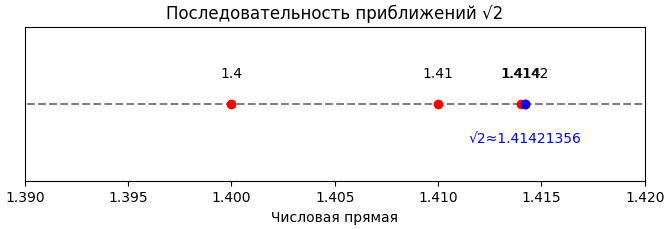
\includegraphics[scale=0.5]{images/img11}
	$$
	Метрическое пространство называется \textbf{полным}, если в нем всякая
	фундаментальная последовательность сходится. Полное нормированное
	пространство называется \textbf{банаховым пространством}.
	\\\\
	Например, 
	\begin{itemize}
		\item $C[a,b]$ с нормой $\Norm{x} = \underset{t \in [a,b]}{\max} |x(t)|$;
		\item $l_p$ с нормой $\Norm{x} = \left(\sum_{k=1}^{\infty}|x_k|^p\right)^{1/p}$.
	\end{itemize} 
	Пусть в банаховом пространстве $E$ действует отображение $f$. Точка $x^*\in E$ называется \textbf{неподвижной точкой отображения $f$}, если \begin{equation*}
		f(x^*) = x^*.
	\end{equation*}
	Таким образом, неподвижные точки $f$ -- это решения уравнения \begin{equation*}
		x = f(x).
	\end{equation*}
	Среди отображений $f: E \to F$ выделим класс отображений специального вида.
	Отображение $f$ является \textbf{сжимающим (сжатием)}, если существует константа $\alpha \in (0,1)$ такая, что
	\begin{equation*}
		\Norm{f(x) - f(y)}_F\leq \alpha \Norm{x - y}_E,\ \forall x ,y \in E,
	\end{equation*}
	а число $\alpha$ называется \textbf{коэффициентом сжатия}.
	\begin{theorem}
		[Банаха о неподвижной точке сжимающего отображения]
		Пусть
		\begin{itemize}
			\item в банаховом пространстве $E$ задано замкнутое множество $M$;
			\item отображение $f$ отображает $M$ в себя;
			\item отображение $f$ на $M$ является сжимающим с коэффициентом сжатия $\alpha$.
		\end{itemize}
		Тогда 
		\begin{itemize}
			\item на множестве $M$ отображение $f$ имеет единственную неподвижную точку $x^*$;
			\item неподвижная точка $x^*$ может быть найдена методом последовательных приближений
			\begin{equation*}
				x_n = f(x_{n-1}),\ n=1,2,\ldots,
			\end{equation*}
			где $(x_n) \subset M$, $x_ n \xrightarrow[n\to\infty]{}x^*$;
			\item справедлива оценка скорости сходимости
			\begin{equation*}
				\Norm{x_n - x^*} \leq \dfrac{\alpha^n}{1 - \alpha} \Norm{x_0 - x_1}.
			\end{equation*}
		\end{itemize}
	\end{theorem}
	Пусть задана система линейных уравнений 
	\begin{equation}
		\label{sle-1}
		Ax = b,
	\end{equation}
	где $A$  -- невырожденная квадратная матрица размерности $m\times m$, то есть существует единственное решение, $b$ -- это вектор неоднородности, а $x$ -- неизвестный вектор решений. Представим эту систему в эквивалентном виде
	\begin{equation}
		\label{sle-2}
		x = Cx + d,
	\end{equation}
	где $C = (c_{ij})$ -- это матрица размерности $m\times m$, а $d$ -- это вектор. Тогда найдя решение системы \eqref{sle-2}, мы найдем решение системы \eqref{sle-1}.  Если представить, что задано отображение $F : \mathbb R^m \to \mathbb R^m$ такое, что
	\begin{equation*}
		F(x) = Cx + d,
	\end{equation*}
	то уравнение \eqref{sle-2} представимо в виде
	\begin{equation}
		x = F(x),
	\end{equation}
	решением которого будет являться неподвижная точка отображения $F$. Следовательно, решение системы \eqref{sle-2} свелось к тому, что мы должны выяснить, является ли отображение $F$ сжатием. И если это так, то к отысканию решения системы \eqref{sle-2} можно применить принцип сжимающих отображений. 
	\begin{theorem}
		Если для системы линейных уравнений \eqref{sle-2} матрица $C$ такая, что выполняется хотя бы одно из условий
		\begin{equation}
			\label{conditions-1}
			\Norm{C}_1 = \underset{1 \leq i \leq m}{\max} \sum_{j=1}^{m}|c_{ij}| < 1, \text{ или } \Norm{C}_2 = \underset{1 \leq j \leq m}{\max} \sum_{i=1}^{m}|c_{ij}| < 1,
		\end{equation}
		то существует единственное решение системы \eqref{sle-2} (следовательно и \eqref{sle-1}), которое может быть найдено методом последовательных приближений
		\begin{equation}
			x_i ^{(n+1)} = \sum_{j=1}^m c_{ij} x_j ^{(n)} + d_i
		\end{equation}
		при любом заданном начальном приближении $x^{(0)}\in \mathbb R^m$.
	\end{theorem}
	\noindent Условия \eqref{conditions-1} являются достаточными, но не необходимыми. Пусть матрица $C$ является симметричной. Тогда принцип сжимающих отображений сходится к решению тогда и только тогда, когда
	\begin{equation*}
		\Norm{C}_3 = |\underset{i}{\max \lambda _i (C)}| < 1.
	\end{equation*}
	Чтобы представить систему \eqref{sle-1} в виде \eqref{sle-2} таким образом, чтобы метод последовательных приближений сходился, матричное уравнение можно записать следующим образом
	\begin{equation}
		x = \underbrace{\left(E - \dfrac{A^T A}{\lambda(A^T A)} \right)}_{C}x + \underbrace{\dfrac{A^T b}{\lambda (A^T A)}}_{d}, 
	\end{equation}
	в таком случае $|\lambda_i(C)| < 1$, а значит будет сходимость.
	\noindent
	Пусть задано линейное неоднородное интегральное уравнение Фредгольма второго рода
	\begin{equation}
		\label{fie-1}
		x(t) -\lambda\int\limits_a^b \mathcal K(t,s)x(s)ds = y(t),\ t \in [a,b].
	\end{equation}
	Оно имеет единственное непрерывное на $[a,b]$ решение, если $\lambda$ не является собственным значением интегрального оператора.
	Уравнение \eqref{fie-1} можно представить в виде
	\begin{equation*}
		\label{fie-2}
		x = F(x),\ F(x) = \lambda\int\limits_a^b \mathcal K(t,s)x(s)ds + y(t),
	\end{equation*}
	причем отображение $F$ отображает множество функций, заданных на $[a,b]$ в себя. Таким образом, решением уравнения \eqref{fie-2} является неподвижная точка отображения $F$. Для применения принципа сжимающих отображений необходимо 
	\begin{itemize}
		\item задать банахово пространство функций;
		\item проверить, что отображение $F$ сжимающее.
	\end{itemize}
	\begin{theorem}
		Пусть в банаховом пространстве $E = C[a,b]$ ядро $\mathcal K(t,s)$ -- непрерывная на $\Omega = [a,b]\times [a,b]$ функция и $M = \underset{(t,s)\in \Omega}{\max} |\mathcal K(t,s)|$. Тогда для любого $\lambda$ такого, что 
		\begin{equation*}
			|\lambda| < \dfrac{1}{M(b-a)},
		\end{equation*}
		существует единственное решение уравнения \eqref{fie-1} для любой правой части $y(t) \in C[a,b]$, которое может быть найдено методом последовательных приближений по формуле
		\begin{equation}
			x_n(t) = \lambda\int\limits_a^b \mathcal K(t,s)x_{n-1}(s)ds + y(t)
		\end{equation}
	\end{theorem}
	\noindent
	Пусть задано линейное неоднородное интегральное уравнение Вольтерра второго рода
	\begin{equation}
		\label{vie-1}
		x(t) -\lambda\int\limits_a^t \mathcal K(t,s)x(s)ds = y(t).
	\end{equation}
	\begin{theorem}
		Пусть в банаховом пространстве $E = C[a,b]$ ядро $\mathcal K(t,s)$ -- непрерывная по переменным $t$ и $s$ функция. Тогда для любого $\lambda$ из поля $P$ существует единственное решение уравнения \eqref{vie-1} для любой правой части $y(t) \in C[a,b]$, которое может быть найдено методом последовательных приближений по формуле
		\begin{equation}
			x_n(t) = \lambda\int\limits_a^t \mathcal K(t,s)x_{n-1}(s)ds + y(t)
		\end{equation}
	\end{theorem}
	\noindent
	Ядро $\mathcal K(t,s)$ называется \textbf{вырожденным}, если оно имеет вид
	\begin{equation*}
		\mathcal K(t,s) = \sum_{i=1}^{m} a_i(t) b_i(s),
	\end{equation*}
	где $a_i(t)$, $b_i(s)$ -- равномерно непрерывные, линейно независимые функции. Интегральные уравнения Фредгольма второго рода с вырожденным ядром можно свести к решению системы линейных алгебраических уравнений. Интегральные уравнения Вольтерра второго рода с вырожденным ядром можно свести к решению системы линейных обыкновенных дифференциальных уравнений. 
	\\\\
	При выполнении условий теоремы для интегрального уравнения Фредгольма решение можно также искать с помощью метода резольвент (это следует из теории обратимых линейных ограниченных операторов). Функция
	\begin{equation}
		R(t,s;\lambda)=\sum_{n=1}^{\infty} \lambda^{n-1} \mathcal K_n(t,s),
	\end{equation}
	называется \textbf{резольвентой} ядра $\mathcal K(t,s)$, при этом
	\begin{equation}
		\mathcal K_n(t,s) = \int\limits_a^b \mathcal K(t,\tau) \cdot \mathcal K_{n-1}(\tau, s)d\tau,\ K_1(t,\tau) = K(t,\tau).
	\end{equation}
	Таким образом, решение уравнения \eqref{fie-1} по методу резольвент представимо в виде
	\begin{equation}
		x(t) = y(t) + \lambda \int\limits_a^b R(t,s;\lambda)y(s)ds.
	\end{equation}
	По аналогии определяется решение методом резольвент для интегрального уравнения Вольтерра.
	
	\section{Компактные множества и компактные операторы}
	Пусть $E$ -- банахово пространство. Множество $M \subset E$ называется \textbf{компактным}, если из каждое последовательности $(x_n)\subset M$ можно выбрать сходящуюся подпоследовательность $(x_{n_k})\subset (x_n)$, предел которой принадлежит $M$.
	\\\\
	Компактное множество в банаховом пространстве ограничено, замкнуто и полно.
	\\\\
	Множество $S _ \epsilon \subset E$ называется \textbf{$\epsilon$-сетью}, $\epsilon > 0$ для множества $M \subset E$, если для любого $x \in M$ найдется $s \in S_\epsilon$ такое, что $\Norm{x -s }< \epsilon$. 
	\\\\
	Например на плоскости $M = [-5, 5]\times [-5,5]$ целочисленные точки образуют сеть радиуса $\epsilon = \sqrt 2 / 2$
	$$
		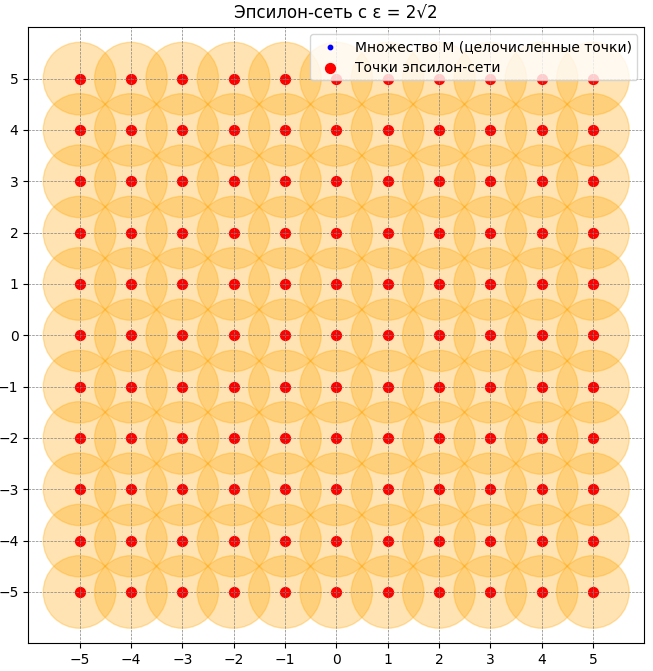
\includegraphics[scale=0.5]{images/img26}
	$$
	Множество $M\subset E$ называется \textbf{вполне ограниченным}, если для любого $\epsilon > 0$ в $E$ существует конечная $\epsilon$-сеть для множества $M$.
	\begin{theorem}
		[критерий компактности Хаусдорфа]
		Пусть $M \subset E$ -- множество в банаховом пространстве. Тогда $M$ компактно тогда и только тогда, когда $M$ замкнуто и вполне ограничено. 
	\end{theorem}
	\noindent
	В конечномерном пространстве множество $M$ компактно тогда и только тогда, когда оно замкнуто и ограничено.
	\\\\
	Множество $M \subset E$ называется \textbf{предкомпактным}, если его замыкание $\overline M$ компактно.
	\begin{theorem}
		Предкомпактное множество в банаховом пространстве компактно тогда и только тогда, когда оно замкнуто.
	\end{theorem}
	\begin{theorem}
		Множество $M$ предкомпактно тогда и только тогда, когда оно вполне ограничено.
	\end{theorem}
	\noindent
	Пусть $X$ и $Y$ -- банаховы пространства. Линейный оператор $A : X \to Y$ называется \textbf{компактным (вполне непрерывным)}, если он отображает всякое ограниченное множество пространства $X$  в предкомпактное множество пространства $Y$.
	\\\\
	Рассмотрим оператор $A : C[a,b]\to C[a,b]$ такой, что 
	\begin{equation*}
		Ax(t) = \int\limits_a^b \mathcal K(t,s), x(s)dx.
	\end{equation*}
	Пусть $\mathcal K(t,s) \in C([a,b]\times [a,b])$ -- непрерывное ядро интегрального оператора Фредгольма. Можно доказать, что интегральный оператор Фредгольма с непрерывным ядром компактен. В частности интегральный оператор Фредгольма (и Вольтерра) с вырожденным ядром является компактным. Ядро $\mathcal K(t,s)$ называется \textbf{вырожденным}, если оно имеет вид
	\begin{equation*}
		\mathcal K(t,s) = \sum_{i=1}^{m} a_i(t) b_i(s),
	\end{equation*}
	где $a_i(t)$, $b_i(s)$ -- равномерно непрерывные, линейно независимые функции.
	\begin{theorem}
		Пусть $X,Y$ -- банаховы пространства, а оператор $A:X\to Y$ является компактным. Тогда сопряженный оператор $A^* : X^* \to Y^*$ также является компактным.
	\end{theorem}
	\noindent
	Пусть $A$  -- это компактный оператор, заданный на банаховом пространстве $X$. Рассмотрим в $X$ линейное уравнение второго рода
	\begin{equation}
		\label{eq-II}
		x - Ax = y,
	\end{equation}
	соответствующее ему однородное уравнение 
	\begin{equation}
		\label{heq-II}
		z - Az = 0,
	\end{equation}
	сопряженное уравнение 
	\begin{equation}
		\label{seq-II}
		u - A^*u = g,
	\end{equation}
	и однородное сопряженное уравнение 
	\begin{equation}
		\label{sheq-II}
		v - A^* v = 0.
	\end{equation}
	Известно также, что $A^*$ является компактным на $X^*$.
	\begin{theorem}
		Множество значений оператора $I - A$ замкнуто в $X$, и, соответственно $I-A^*$ -- в $X^*$.
	\end{theorem}
	\noindent
	Следующие теоремы составляют содержание теории Рисса-Шаудера, являющейся обобщением фредгольмовской теории интегральных уравнений.
	\begin{theorem}[первая теорема Фредгольма]
		Пусть $A$ -- компактный оператор, заданный на банаховом пространстве $X$. Тогда следующие утверждения эквивалентны
		\begin{enumerate}
			\item уравнение \eqref{eq-II} имеет решение при любой правой части $y \in X$;
			\item уравнение \eqref{heq-II} имеет только нулевое решение;
			\item уравнение \eqref{seq-II} разрешимо при любом $g \in X^*$;
			\item уравнение \eqref{sheq-II} имеет только нулевое решение.
		\end{enumerate}
		Если выполнено одно из условий, то операторы $I-A$, $I-A^*$ непрерывно обратимы.
	\end{theorem}
	\begin{theorem}[вторая теорема Фредгольма]
		Пусть $A$ -- компактный оператор, заданный на банаховом пространстве $X$. Тогда однородные уравнения \eqref{heq-II}, \eqref{sheq-II} имеют одинаковое число линейно независимых решений.
	\end{theorem}
	\begin{theorem}[вторая теорема Фредгольма]
		Пусть $A$ -- компактный оператор, заданный на банаховом пространстве $X$. Для того, чтобы уравнение второго рода \eqref{eq-II} имело хотя бы одно решение при заданной правой части $y \in X$, необходимо и достаточно, чтобы для любого решения $v$ уравнения \eqref{sheq-II} выполнялось условие $(v,y) = 0$, то есть правая часть $y \in X$ должна быть ортогональна всем линейно независимым решениям уравнения \eqref{sheq-II}.
	\end{theorem}
	Рассмотрим в пространстве $L_2[a,b]$ интегральное уравнение Фредгольма второго рода
	\begin{equation}
		x(t) - \int\limits_a^b \mathcal K(t,s)x(s)ds = y(t),
	\end{equation}
	где 
	\begin{equation*}
		\label{feq-II}
		\int\limits_a^b \int\limits_a^b | \mathcal K(t,s)|^2ds dt < \infty,
	\end{equation*}
	соответствующее однородное уравнение
	\begin{equation}
		\label{hfeq-II}
		x(t) - \int\limits_a^b \mathcal K(t,s)x(s)ds = 0.
	\end{equation}
	Поскольку $L_2[a,b]$ -- гильбертово пространство и $(L_2[a,b])^*$ линейно изоморфно $L_2[a,b]$, то соответствующие сопряженные уравнения можно записать опять же на элементах пространства $L_2[0,1]$
	\begin{equation}
		\label{sfeq-II}
		u(t) - \int\limits_a^b \mathcal K(s,t)u(s)ds = g(t),
	\end{equation}
	\begin{equation}
		\label{hsfeq-II}
		u(t) - \int\limits_a^b \mathcal K(s,t)u(s)ds = 0.
	\end{equation}
	\begin{theorem}
		[альтернатива Фредгольма]
		Пусть $\mathcal K(t,s)$ -- такое ядро, при котором интегральный оператор компактен в $L_2[a,b]$. Тогда возможны лишь два случая
		\begin{enumerate}
			\item однородные уравнения \eqref{hfeq-II}, \eqref{hsfeq-II} имеют только нулевые решения; уравнения \eqref{feq-II}, \eqref{sfeq-II} разрешимы для любой правой части и имеют единственные решения;
			\item однородное уравнение \eqref{hfeq-II} имеет лишь конечное число линейно независимых решений $x_1,\ldots, x_n$. Тогда сопряженное уравнение \eqref{hsfeq-II} имеет то же количество линейно независимых решений $u_1,\ldots, u_n$. Неоднородное уравнение \eqref{feq-II} разрешимо, если 
			\begin{equation*}
				\int\limits_a^b u_i(t) y(t)dt = 0,\ i = 1,\ldots, n,
			\end{equation*}
			 и его решение
			 \begin{equation*}
			 	x(t) = \sum_{k=1}^{n}C_k x_k + x_0(t),
			 \end{equation*}
			 где $C_1,\ldots, C_n$ -- произвольные постоянные; $x_0$ -- некоторое частное решение неоднородного уравнения \eqref{feq-II}.
		\end{enumerate}
	\end{theorem}
	\begin{theorem}
		Если ядро $\mathcal K(t,s) \in C([a,b]\times [a,b])$, то для уравнения \eqref{feq-II} справедлива альтернатива Фредгольма.
	\end{theorem}
	\chapter{Математическое моделирование}
	\section{Методы решения задачи Коши для дифференциальных уравнений с частными производными}
	\textbf{Задача Коши для уравнения второго порядка с двумя независимыми переменными} в области $D\in\mathbb R^2$ формулируется как:
	\begin{equation} \label{2.1.1}
		Lu \equiv a_{11}\dfrac{\partial ^ 2u}{\partial x^2} + 2a_{12}\dfrac{\partial ^ 2u}{\partial x \partial y} + a_{22}\dfrac{\partial^2 u}{\partial y^2} + a\dfrac{\partial u}{\partial x} + b\dfrac{\partial u}{\partial y} + cu = f(x,y),
	\end{equation}
	\begin{equation} \label{2.1.2}
		\begin{gathered}
			u|_{(x, y)\in\textup{Г}} = \varphi(x, y),\\
			\dfrac{\partial u}{\partial \Vec{n}}\Bigr|_{(x, y)\in\textup{Г}} = \psi(x, y),
		\end{gathered}
	\end{equation}
	где $D$ --- плоская область в $\mathbb R^2$, $\Gamma$ --- линия внутри области $D$, $u \in C^2(D)$, $\Gamma\in C^2$, $\varphi$ и $\psi$ --- функции, заданные на линии $\Gamma$.
	\begin{center}
		\begin{tikzpicture} [scale=1.5]
			\draw (-0.1, -0.1) node {0};
			\draw (1.65, 1.1) node {$\Vec{n}$};
			\draw (1.25, 1.65) node {$D$};
			\draw (2.4, 1.3) node {Г};
			\draw [<->,thick] (0,2) node (yaxis) [above] {$y$}
			|- (3.5,0) node (xaxis) [right] {$x$};
			\draw plot[smooth, tension=.7] coordinates {(0.5,0.5) (0.25, 1) (0.75, 1.8) (1.25, 2) (2.5, 1.9) (3, 1.4) (2.9, -0.25) (1.5, -0.1) (0.5,0.5)};
			\draw plot[smooth, tension=.7] coordinates {(0.25, 1) (1.5, 0.75) (3, 1.4)};
			\draw[->, thick](1.5,0.75) -- (1.4, 1.2);
		\end{tikzpicture}
	\end{center}
	Пусть
	\begin{enumerate}
		\item $V_1$(Г) --- метрическое пространство начальных функций $\varphi$ с метрикой $\rho_1(\varphi_1, \varphi_2)$;
		\item $V_2$(Г) --- метрические пространство начальных функций $\psi$ с метрикой $\rho_2(\psi_1, \psi_2)$;
		\item $V$(D) --- метрическое пространство  функций $u$, в котором задано решение задачи \eqref{2.1.1}, \eqref{2.1.2}, с метрикой $\rho_3(u_1, u_2)$.
	\end{enumerate}
	Если пространства нормированные, то
	\[
	\rho_1(\varphi_1, \varphi_2) = \|\varphi_1 - \varphi_2\|_{V_1},\
	\rho_2(\psi_1, \psi_2) = \|\psi_1 - \psi_2\|_{V_2},\
	\rho_3(u_1, u_2) = \|u_1 - u_2\|_V.
	\]
	Рассмотрим две задачи Коши с различными начальными функциями
	\begin{equation} \label{2.1.3}
		L(u_i) = f,
	\end{equation}
	\begin{equation} \label{2.1.4}
		\begin{gathered}
			u_i|_{(x, y)\in\textup{Г}} = \varphi_i,\\ \dfrac{\partial u_i}{\partial \Vec{n}}\Bigr|_{(x, y)\in\textup{Г}} = \psi_i,
		\end{gathered}\;\;\; i = 1, 2
	\end{equation}
	Решение задачи \eqref{2.1.3}, \eqref{2.1.4} называется \textbf{устойчивым по начальным данным}, если:
	\begin{equation}\label{2.1.5}
		\forall\varepsilon>0\;\exists\delta>0: \rho_1(\varphi_1, \varphi_2) < \delta,\; \rho_2(\psi_1, \psi_2) < \delta \Rightarrow \rho_3(u_1, u_2) < \varepsilon
	\end{equation}
	Это означает, что с малым изменением начальных параметров, решение также изменяется на малую величину.
	\\\\
	Итак, задача \eqref{2.1.1}, \eqref{2.1.2} считается \textbf{корректно поставленной}, если:
	\begin{enumerate}
		\item {$\forall\varphi\in{V_1},\; \forall\psi\in{V_2}$ существует решение $u\in{V}$;}
		\item {$\forall\varphi\in{V_1},\; \forall\psi\in{V_2}$ решение задачи $u\in V$ единственно;}
		\item {решение $u$ устойчиво по начальным данным.}
	\end{enumerate}
	Пусть задана некоторая область $D=\lbrace- \infty<x<+\infty, |t|\leq T \rbrace.$
	Рассмотрим задачу Коши для однородного уравнения колебания струны
	\begin{equation}
		\label{2.2.1}
		\frac{\partial^2u}{\partial t^2}-a^2\frac{\partial^2u}{\partial x^2}=0, \
		u(x,t) \in C^2(D),
	\end{equation}
	\begin{equation}
		\label{2.2.2}
		u|_{t=0} = \varphi(x),\ -\infty<x<+\infty, \ \varphi \in C^2(\mathbb R),
	\end{equation}
	\begin{equation}
		\label{2.2.3}
		\dfrac{\partial u}{\partial t}\Bigr|_{t=0} = \psi(x),\  -\infty<x<+\infty, \ \psi \in C^1(\mathbb R),
	\end{equation}
	где $a=\sqrt{\dfrac{N}{p}}$, $N$ -- натяжение струны, $p$ -- линейная плотность струны, $t$ -- временная переменная, $x$ -- пространственная переменная.
	Уравнение \eqref{2.2.1} описывает колебания бесконечной струны (под струной понимают тонкую, упругую нить),
	$u(x, t)$ -- задаёт отклонение (смещение) точки с координатой $x$ в момент времени $t$, т.е. задаёт график колебания струны в момент времени $t$.
	Уравнение \eqref{2.2.2} задаёт положение струны в начальный момент времени.
	Уравнение \eqref{2.2.3} задаёт скорость в начальный момент времени.\\\\
	Задача Коши \eqref{2.2.1}-\eqref{2.2.3} является корректно поставленной.
	\textit{Метод характеристик} для построения решения задачи Коши состоит в следующем:
	\begin{enumerate}
		\item
		Уравнение приводится к каноническому виду.
		\item
		Находится общее решение.
		\item
		Определяется явный вид функций из условий (\ref{2.2.2}) и (\ref{2.2.3}).
	\end{enumerate}
	По методу характеристик можно получить решение в виде
	\begin{equation}\label{2.2.4}
		u(x,t)=\frac{\varphi(x-at)+\varphi(x+at)}{2}+\frac{1}{2a}\int\limits_{x-at}^{x+at}\psi(\xi)d\xi
	\end{equation}
	Формула \eqref{2.2.4} называется \textbf{формулой Д'Аламбера} для решения задачи Коши волнового уравнения (для одномерного случая).
	\\\\
	На плоскости $Oxy$ рассмотрим линию $y=g(x)$, которая является достаточно гладкой и удовлетворяет условию, что линии $x=x_0$ и $y=y_0$ пересекают её в одной точке.
	\\\\
	Рассмотрим обобщенную задачу Коши для уравнения гиперболического типа
	\begin{gather}
		\label{2.8.1}
		\pderivtwo{u}{x}{y} + a(x,y)\pderiv{u}{x} +b(x,y)\pderiv{u}{y} + c(x,y)u = f(x,y),\\
		\label{2.8.2}
		u|_{y=g(x)} = \varphi(x),\\
		\label{2.8.3}
		\pderiv{u}{y}\Bigr|_{y=g(x)} = \psi(x).
	\end{gather}
	При этом $\varphi \in C^2[x_1; x_0], \: \psi \in C^1[x_1,x_0]$.\\
	\begin{center}
		\begin{tikzpicture} [scale=1.5]
			\draw (1.2,0.6) node[rotate=-3] {$y=g(x)$};
			\draw (-2.8, 3.6) node {$y_0$};
			\draw (2.8, -0.2) node {$x_0$};
			\draw (1, 2.3) node {$\Omega$};
			\draw (3.2, 3.6) node {$M(x_0,y_0)$};
			\draw (-0.6, 3.6) node {$P(x_1,y_0)$};
			\draw (3.2, 1) node {$Q(x_0,y_1)$};
			\draw[thick] (-2.8,3.4) -- (2.8,3.4);
			\draw[thick] (2.6,-0.2) -- (2.6,3.6);
			\draw (-1.2,3.6) .. controls (-1.2,0.8) .. (2.8,0.8);
			\draw [->, thick] (-3,0)-- (3.5,0) node (xaxis)[below] {$x$};
			\draw [->, thick] (-2.5,-0.2) -- (-2.5,4) node (yaxis)[left] {$y$};
		\end{tikzpicture}
	\end{center}
	Необходимо построить решение в точке $M(x_0,y_0)$.\\\\
	Для задачи \eqref{2.8.1}-\eqref{2.8.3} линии $x=x_0$ и $y=y_0$ являются характеристиками.\\\\
	Введём дифференциальный оператор $Lu$ и сопряжённый к нему $L^*v$:
	$$ Lu = \pderivtwo{u}{x}{y} + a(x,y)\pderiv{u}{x} +b(x,y)\pderiv{u}{y} + c(x,y)u, $$
	$$ L^*v = \pderivtwo{v}{x}{y} -\pderiv{ }{x}(a(x,y)v) -\pderiv{ }{y}(b(x,y)v) + c(x,y)v. $$
	ля того, чтобы решить задачу \eqref{2.8.1}-\eqref{2.8.3} \textbf{методом Римана} необходимо:
	\begin{enumerate}
		\item выписать из исходного уравнения задачу Гурса \begin{equation}
			\begin{gathered}
				\label{2.8.6}
				\begin{cases}
					L^*v=0,\\
					v|_{y=y_0} = e^{\int\limits_{x_0}^x b(x,y_0)dx},\\
					v|_{x=x_0} = e^{\int\limits_{y_0}^y a(x_0,y)dy},\\
					v(x_0,y_0)=1,
				\end{cases}
			\end{gathered}
		\end{equation} для функции Римана; эта задача имеет единственное решение;
		\item решить эту задачу (найти функцию $v=v(x,y, x_0, y_0)$);
		\item найти решение исходной задачи по формуле Римана для обобщенной задачи Коши
		\begin{equation}
			\begin{gathered}
				\label{2.8.7}
				u(x_0,y_0) = \frac{1}{2}(uv)\Bigr|_P + \frac{1}{2}(uv)\Bigr|_Q+\\+
				\frac{1}{2}\int\limits_{PQ}\left(v\pderiv{u}{x} - u\pderiv{v}{x} + 2buv\right)dx -
				\left(v\pderiv{u}{y} - u\pderiv{v}{y} + 2auv\right)dy +
				\int\limits_\Omega vfdxdy
			\end{gathered}
		\end{equation}
	\end{enumerate}
	Пусть задана некоторая область $D=\{-\infty<x<+\infty\text{, } t>0\}$. Рассмотрим задачу Коши для однородного уравнения теплопроводности
	\begin{equation}\label{2.14.1}
		\begin{cases}
			\pderiv{u}{t}=\alpha\pderiv{^2u}{x^2}+\beta\pderiv{u}{x}+\gamma u\text{, } \\
			u|_{t=0}=\varphi(x)
		\end{cases}
	\end{equation}
	Введём пространства:
	$$V_1= \{\varphi\in C_0(-\infty<x<+\infty)\}$$
	$$V=\{u\in C^2(D)\cap C(\overline{D})\}$$
	Алгоритм решения задачи Коши \eqref{2.14.1} \textbf{методом интегральных преобразований Фурье} следующий:
	\begin{enumerate}
		\item вместо функции $u(x,t)$ решается задача относительно образа этой функции 
		\begin{equation*}
			\hat{u}(\lambda,t)=\frac{1}{\sqrt{2\pi}}\int\limits_{-\infty}^{+\infty}u(x,t)e^{i\lambda x}dx,
		\end{equation*}
		который получается в результате применения прямого преобразования Фурье к $u(x,t)$;
		\item задача относительно образа $\hat{u}(\lambda,t)$ сводится к линейному обыкновенному дифференциальному уравнению с постоянными коэффициентами;
		\item решив задачу относительно образа функции, с помощью обратного преобразования Фурье можно получить решение задачи Коши $u(x,t)$.
	\end{enumerate}
	По методу интегральных преобразований Фурье получаются следующие формулы для решения задачи \eqref{2.14.1}.
	\\\\
	Функция 
	\begin{equation*}
		G(x-y,t)=\frac{e^{\gamma t}}{2\sqrt{\alpha\pi t}}e^{-\frac{(\beta t+x-y)^2}{4\alpha t}}
	\end{equation*}
	называется \textbf{фундаментальным решением уравнения теплопроводности}.
	\\\\
	Тогда решение задачи Коши представляется в виде
	\begin{equation}
		u(x,t)=\int\limits_{-\infty}^{+\infty}\varphi(y)G(x-y,t)dy
	\end{equation}
	Рассмотрим стандартную задачу Коши для теплопроводности стержня
	\begin{equation}
		\begin{gathered}
			\pderiv{u}{t}=a^2\pderiv{^2u}{x^2},\\
			u|_{t=0}=\varphi(x).
		\end{gathered}
	\end{equation}
	Используя фундаментальное решение, получим функцию
	\begin{equation}
		\label{eq:pois-int}
		u(x,t)=\frac{1}{2a\sqrt{\pi t}}\int\limits_{-\infty}^{+\infty}\varphi(y)e^{-\frac{(x-y)^2}{4a^2t}}dy
	\end{equation}
	Функция \eqref{eq:pois-int} называется \textbf{интегралом Пуассона}.
	\section{Дифференциальные модели. Постановка краевых задач для дифференциальных уравнений с частными производными}
	На плоскости рассмотрим полуограниченную полосу
	$D=\{0<x<l\text{, } t>0\}.$
	На ней поставлена \textbf{задача Коши для волнового уравнения}
	\begin{equation}
		\begin{gathered}
			\pderiv{^2u}{t^2}=a^2\pderiv{^2u}{x^2}+f(x,t),\\
			u|_{t=0}=\varphi(x)\text{, } 0\leq x\leq l,\\
			\pderiv{u}{t}\Bigr|_{t=0}=\psi(x)\text{, } 0\leq x\leq l,
		\end{gathered}
	\end{equation}
	при этом $f_{xx}\in C(\overline{D})\text{, } \varphi\in C^2(0\leq x\leq l)\text{, } \psi\in C^1(0\leq x\leq l).$
	Волновое уравнение описывает процесс колебания струны. Т.е. $u(x,t)$ -- это смещение точки с координатой $x$ в момент времени $t$. Первое начальное условие задаёт профиль струны в начальный момент времени, второе начальное условие задаёт скорость в начальный момент времени.
	\begin{table}[h!]
		\renewcommand{\arraystretch}{1.4}
		\begin{tabular}{|p{5.5cm}|p{4.5cm}|p{7cm}|}
			\hline
			\textbf{Вид граничных условий} & \textbf{Физический смысл} & \textbf{Условия согласования} \\
			\hline
			Первого рода $$u|_{x=0}=\mu_1(t),\ t \geq 0,$$ $$u|_{x=l}=\mu_2(t), \ t \geq 0.$$
			& 
			Концы струны закреплены на определённой высоте, причём высота может меняться со временем.
			& 
			$$\varphi(0)=\mu_1(0),\ \varphi(l)=\mu_2(0)$$  $$\psi(0)=\mu_1'(0),\ \psi(l)=\mu_2'(0)$$ \\
			\hline
			
			{Второго рода} $$\begin{gathered}
				\pderiv{u}{x}\Bigr|_{x=0}=\mu_1(t)\text{, } t\geq 0,\\
				\pderiv{u}{x}\Bigr|_{x=l}=\mu_2(t)\text{, } t\geq 0,
			\end{gathered}$$ 
			& 
			На концы струны действуют заданные силы.
			& 
			$$\varphi'(0)=\mu_1(0)\text{, } \varphi'(l)=\mu_2(0),$$
			$$\psi'(0)=\mu_1'(0)\text{, }\psi'(l)=\mu_2'(0).$$ \\
			\hline
			
			{Третьего рода} $$\begin{gathered}
				\pderiv{u}{x}-h(t)u\Bigr|_{x=0}=\mu_1(t)\text{, } t\geq 0,\\
				\pderiv{u}{x}+h(t)u\Bigr|_{x=l}=\mu_2(t)\text{, } t\geq 0,
			\end{gathered}$$
			& 
			На концы струны действуют упругие силы: концы движутся, но упругие силы возвращают их в исходное положение.
			& 
			$$\varphi'(0)-h(0)\varphi(0)=\mu_1(0),$$
			$$\varphi'(l)+h(0)\varphi(l)=\mu_2(0),$$
			$$\psi'(0)-h'(0)\varphi(0)-h(0)\psi(0)=\mu_1'(0),$$
			$$\psi'(l)+h'(0)\varphi(l)+h(0)\psi(l)=\mu_2'(0).$$ \\
			\hline
		\end{tabular}
	\end{table}

	При этом $\mu_i\in C^2(t\geq 0)$, $i=1,2$; $h\in C^1(t\geq 0)$, $h(t)>0$. Необходимо найти функцию
	$u\in C^2(\overline{D})$, удовлетворяющую задаче Коши и граничным условиям. Для корректной постановки задачи необходимо выполнение условий согласования.
	
	
	Пусть теперь поставлена \textbf{задача Коши для уравнения теплопроводности}
	\begin{equation}
		\begin{gathered}
			\pderiv{u}{t}=a^2\pderiv{^2u}{x^2}+f(x,t),\\
			u|_{t=0}=\varphi(x)\text{, } 0\leq x\leq l,
		\end{gathered}
	\end{equation}
	при этом $f\in C(\overline{D})$, $\varphi\in C(0\leq x\leq l)$. Уравнение теплопроводности описывает процесс распространения тепла в тонком стержне. Функция $u(x,t)$ задаёт температуру стержня в сечении $x$ в момент времени $t$. Начальное условие задаёт температуру стержня в каждом сечении $x$ в начальный момент времени $t=0$.
	\begin{table}[h!]
		\renewcommand{\arraystretch}{1.4}
		\begin{tabular}{|p{5.5cm}|p{4.5cm}|p{7cm}|}
			\hline
			\textbf{Вид граничных условий} & \textbf{Физический смысл} & \textbf{Условия согласования} \\
			\hline
			{Первого рода} 
			$$\begin{gathered}
				u|_{x=0}=\mu_1(t),\ t \geq 0,\\
				u|_{x=l}=\mu_2(t),\ t \geq 0
			\end{gathered}$$
			&
			На концах стержня поддерживаются заданные температуры $\mu_1(t)$ и $\mu_2(t)$.
			&
			$$\varphi(0)=\mu_1(0),\ \varphi(l)=\mu_2(0)$$
			\\
			\hline
			
			{Второго рода}
			$$\begin{gathered}
				\pderiv{u}{x}\Bigr|_{x=0}=\mu_1(t),\ t\geq 0,\\
				\pderiv{u}{x}\Bigr|_{x=l}=\mu_2(t),\ t\geq 0
			\end{gathered}$$
			&
			На концах стержня задаётся тепловой поток.
			&
			$$\varphi'(0)=\mu_1(0),\ \varphi'(l)=\mu_2(0)$$
			\\
			\hline
			
			{Третьего рода}
			$$\begin{gathered}
				\pderiv{u}{x}-h(t)u\Bigr|_{x=0}=\mu_1(t),\ t\geq 0,\\
				\pderiv{u}{x}+h(t)u\Bigr|_{x=l}=\mu_2(t),\ t\geq 0
			\end{gathered}$$
			&
			На концах стержня происходит теплообмен с внешней средой.
			&
			$$\varphi'(0) - h(0)\varphi(0) = \mu_1(0),$$ 
			$$\varphi'(l) + h(0)\varphi(l) = \mu_2(0)$$
			\\
			\hline
		\end{tabular}
	\end{table}
	
	При этом $\mu_i\in C(t\geq 0)$, $i=1,2$; $h\in C(t\geq 0)$. Необходимо найти функцию
	$u\in C_{x,t}^{2,1}(D)\cap C^1(\overline{D})$, удовлетворяющую задаче Коши с граничными условиями.
	\\\\
	Деление на типы смешанных задач происходит по виду граничных условий.
	\\\\
	Рассмотрим область $D$ с границей $\Gamma  = \delta D$. На ней задана функция $u \in C^2(D)$. 
	\\\\
	Уравнение 
	\begin{equation}
		\Delta u = \pderivt{u}{x} + \pderivt{u}{y} + \pderivt{u}{z} = 0,
	\end{equation}
	называется \textbf{уравнением Лапласа}. Функция, удовлетворяющая уравнению Лапласа, называется \textbf{гармонической функцией}.\\\\
	Уравнение \begin{equation}
		\Delta u = f(x,y,z)
	\end{equation}
	называется \textbf{уравнением Пуассона}.
	
	\begin{table}[h!]
		\renewcommand{\arraystretch}{1.4}
		\begin{tabular}{|p{5.5cm}|p{6cm}|p{5cm}|}
			\hline
			\textbf{Вид задачи и граничные условия} & \textbf{Физический смысл / интерпретация} & \textbf{Особые требования / корректность} \\
			\hline
			
			\textbf{Внутренняя задача Дирихле} 
			$$\begin{gathered}
				\Delta u = f(M),\ M \in D, \\
				u|_{P \in \Gamma} = \varphi(P)
			\end{gathered}$$
			& 
			Внутренняя задача для области $D$ с заданием значений функции $u$ на границе $\Gamma$ (например, фиксированная температура, потенциал и т.п.). 
			&
			Является корректно поставленной: решение существует, единственно и непрерывно зависит от данных. 
			\\
			\hline
			
			\textbf{Внешняя задача Дирихле} 
			$$\begin{gathered}
				\Delta u = f, \\
				u|_{P \in \Gamma} = \varphi(P), \\
				u(M) \underset{M\to\infty}{\rightrightarrows} 0
			\end{gathered}$$
			& 
			Внешняя задача для $D' = \mathbb{R}^3 \setminus D$. Требуется найти функцию $u$, равную $\varphi$ на поверхности $\Gamma$, и стремящуюся к нулю при удалении в бесконечность (например, распределение потенциала вне проводника).
			&
			Требуется условие стремления $u$ к нулю на бесконечности. Задача корректна.
			\\
			\hline
			
			\textbf{Внутренняя задача Неймана} 
			$$\begin{gathered}
				\Delta u = f, \\
				\dfrac{\partial u(P)}{\partial n_P}|_{P\in \Gamma} = \varphi(P)
			\end{gathered}$$
			& 
			Внутренняя задача с заданием нормальной производной на границе (например, заданная плотность потока через поверхность $\Gamma$).
			&
			Единственность решения только с точностью до константы; для существования решения требуется $$\int_\Gamma \varphi(P)\, dS = \int_D f(M)\, dV$$ (условие совместимости).
			\\
			\hline
			
			\textbf{Внешняя задача Неймана}
			$$\begin{gathered}
				\Delta u = f, \\
				\dfrac{\partial u(P)}{\partial n_P}|_{P\in \Gamma} = \varphi(P), \\
				u(M) \underset{M\to\infty}{\rightrightarrows} 0
			\end{gathered}$$
			&
			Внешняя задача для $D' = \mathbb{R}^3 \setminus D$ с заданием нормальной производной на $\Gamma$ и стремлением $u$ к нулю на бесконечности.
			&
			Для существования решения требуется условие совместимости $$\int_\Gamma \varphi(P)\, dS = \int_{D'} f(M)\, dV.$$
			\\
			\hline
		\end{tabular}
	\end{table}
	
	Рассмотрим общую схему метода Фурье (разделения переменных) для решения смешанных задач.
	Рассмотрим смешанную задачу для уравнения гиперболического типа:
	\begin{equation}\label{3.5.1}
		\rho(x)\pderiv{^2u}{t^2}-L(u)=0,
	\end{equation}
	\begin{equation}\label{3.5.2}
		\begin{gathered}
			u|_{t=0}=\varphi(x),\\
			\pderiv{u}{t}\Bigr|_{t=0}=\psi(x),
		\end{gathered}
	\end{equation}
	\begin{equation}\label{3.5.3}
		\begin{gathered}
			\alpha_1\pderiv{u}{x}-\beta_1u\Bigr|_{x=0}=0,\\
			\alpha_2\pderiv{u}{x}+\beta_2u\Bigr|_{x=l}=0,
		\end{gathered}
	\end{equation}
	где
	$$L(u)=\frac{d}{dx}\left(k(x)\frac{du}{dx}\right)-qu.$$
	Решение ищем в виде произведения функций:
	$$u(x,t)=X(x)T(t), \text{ где }X(x)\not\equiv 0,\ T(t)\not\equiv 0.$$
	Подставим это представление в уравнение
	$$\rho(x)T''X-L(X)T=0.$$
	Делим полученное выражение на $\rho XT$ и приравниваем к константе (так как слева и справа функции зависят от разных переменных)
	$$\frac{T''}{T}=\frac{L(X)}{\rho X} = -\lambda.$$
	Отсюда получаем два уравнения:
	\begin{equation}\label{3.5.4}
		T''(t)+\lambda T(t)=0,
	\end{equation}
	\begin{equation}\label{3.5.5}
		L(X(x))+\lambda\rho X(X)=0.
	\end{equation}
	Подставляем $u(x,t) = X(x)T(t)$ в граничные условия и получаем
	\begin{equation}\label{3.5.6}
		\alpha_1X'(0)-\beta_1X(0)=0,
	\end{equation}
	\begin{equation}\label{3.5.7}
		\alpha_2X'(l)+\beta_2X(l)=0,
	\end{equation}
	в силу того, что $T(t) \not \equiv 0$.
	В итоге имеем задачу Штурма-Лиувилля для исходной задачи
	\begin{equation}
		\begin{cases}
			L(X(x))+\lambda\rho X(x)=0,\\
			\alpha_1X'(0)-\beta_1X(0)=0,\\
			\alpha_2X'(l)+\beta_2X(l)=0.
		\end{cases}
	\end{equation}
	Пусть $\lambda_n\geq 0$ -- собственные значения для этой задачи, а $X_n$ -- собственные функции.
	Если $\lambda_0=0$ является собственным значением, то полагаем, что $X_0=1$. Если $\lambda_0=0$ не является собственным значением, то полагаем, что $X_0=0$.\\\\
	Для найденных собственных значений $\lambda_n$ решаем уравнение (\ref{3.5.4}) для $T$:
	$$T_n''(t)+\lambda_nT_n(t)=0$$
	Тогда
	$$T_n(t)=A_n\cos\left(\sqrt{\lambda_n}t\right)+B_n\sin\left(\sqrt{\lambda_n}t\right)$$
	Если $\lambda_0=0$ является собственным значением, то для $T_0$ имеем уравнение $T_0''(t)=0$, и его общее решение имеет вид $T_0=A_0t+B_0$. Тогда имеем для исходного уравнение общее решение вида $u_0=A_0t+B_0$.
	Таким образом имеем множество частных решений:
	$$u_n=\left(A_n\cos\left(\sqrt{\lambda_n}t\right)+B_n\sin\left(\sqrt{\lambda_n}t\right)\right)X_n(x)$$
	Так как исходное уравнение однородно, то решение будем искать как сумму однородного и частных решений:
	$$u(x,t)=A_0t+B_0+\sum\limits_{n=1}^\infty\left(A_ncos\left(\sqrt{\lambda_n}t\right)+B_nsin\left(\sqrt{\lambda_n}t\right)\right)X_n(x)$$
	В данном решении не известны коэффициенты $A_n$ и $B_n$.
	Для их нахождения используются начальные условия (\ref{3.5.2}).
	Подставляем в первое начальное условие:
	$$u|_{t=0}=B_0+\sum\limits_{n=1}^\infty A_nX_n(x)=\varphi(x)$$
	Раскладываем в ряд Фурье по собственным функциям:
	$$\varphi(x) = \sum_{n=1}^\infty \varphi_n X_n(x),\ \varphi_n=\frac{1}{\|X_n\|^2}\int\limits_0^l\varphi(x)\rho(x)X_n(x)dx$$
	Откуда
	$$A_n=\varphi_n\text{, }n=1,2\dots$$
	$$B_0=\varphi_0$$
	Подставляем во второе начальное условие:
	$$\pderiv{u}{t}\Bigr|_{t=0}=A_0+\sum\limits_{n=1}^\infty \sqrt{\lambda_n}B_nX_n(x)=\psi(x)$$
	Раскладываем в ряд по собственным функциям:
	$$\psi(x)=\sum\limits_{n=1}^\infty \psi_nX_n\Rightarrow A_0=\psi_0,\  B_n=\frac{\psi_n}{\sqrt{\lambda_n}}.$$
	Таким образом построили решение:
	$$u(x,t)=\psi_0t+\varphi_0+\sum_{n=1}^\infty\left(\varphi_n\cos\left(\sqrt{\lambda_n}t\right)+\frac{\psi_n}{\sqrt{\lambda_n}}\sin\left(\sqrt{\lambda_n}t\right)\right)X_n(x)$$
	Но, для того, чтобы этот ряд был решением смешанной задачи (\ref{3.5.1})-(\ref{3.5.3}), необходимо, чтобы этот ряд сходился.\\\\
	Возможны два случая:
	\begin{enumerate}
		\item исходное уравнение неоднородное;
		\item граничные условия неоднородные.
	\end{enumerate}
	В первом случае мы сначала выписываем и решаем соответствующую задачу Штурма-Лиувилля для неоднородного уравнения и находим функции $X_n(x)$, а затем представляем решение в виде $$u(x,t) = \sum_{n=1}^\infty X_n(x)T_n(t),$$ и подставляем его в уравнение.
	\\\\
	Во втором случае мы представляем решение задачи в виде
	\begin{equation*}
		u(x,t) = v(x,t) + w(x,t),
	\end{equation*}
	где функция $w(x,t)$ подбирается таким образом, чтобы для $v(x,t)$ можно было сформулировать соответствующую задачу с однородными граничными условиями.
	\section{Задачи для уравнений эллиптического типа}
	Рассмотрим область $D \subset \mathbb R^3$, ограниченную поверхностью $\Gamma = \delta D$ и определим на ней функцию $u(x,y,z):D \to \mathbb R$. Функция $u(x,y,z)$ называется \textbf{гармонической функцией}, если $u\in C^2(D)$ и
	\begin{equation}
		\label{laplaseq-1}
		\Delta u = \pderivt{u}{x} + \pderivt{u}{y} + \pderivt{u}{z} = 0,
	\end{equation}
	а уравнение \eqref{laplaseq-1} называется \textbf{уравнением Лапласа}.
	\\\\
	Рассмотрим свойства гармонических функцией.
	\begin{enumerate}
		\item Пусть функция $u(x,y,z)$ является гармонической в области $D$ ограниченной областью $\Gamma$. Тогда имеем, что
		$$\iint\limits_\Gamma \pderiv{u(P)}{n_P}dS_P=0.$$
		(данное свойство важно для разрешения задачи Неймана, которая задана на поверхности $\Gamma$ значением своих производных).
		\item \textbf{Теорема о среднем}. Пусть $u(x,y,z)$ --- гармоническая функция и $\Gamma_a^M$ -- сфера радиуса $a$ с центром в точке $M$.
		Тогда
		$$u(M)=\frac{1}{|\Gamma_a^M|}\iint\limits_{\Gamma_a^M}u(P)dS_P,$$
		где $|\Gamma_a^M|=4\pi a^2$ -- площадь поверхности сферы.
		\item \textbf{Принцип максимума и минимума для гармонических функций}. Пусть функция $u(x,y,z)$ является гармонической функцией в области $D$, ограниченной поверхностью $\Gamma$, причем $u\in C^2(D)\cap C^1(\overline{D})$. Тогда своего максимального и минимального значения функция достигает на поверхности $\Gamma$, то есть
		$$\min\limits_{M\in\Gamma}u(M)\leq \underset{M\in D}{u(M)}\leq \max\limits_{M\in\Gamma}u(M).$$
	\end{enumerate}
	Уравнение 
	\begin{equation}
		\Delta u = f(x,y,z)
	\end{equation}
	называется \textbf{уравнением Пуассона}.
	\\\\
	Дифференциальные уравнения в частных производных с дифференциальным оператором Лапласа (то есть уравнения Лапласа и Пуассона) называются \textbf{уравнениями эллиптического типа}. Для уравнений эллиптического типа формулируются следующие граничные задачи:
	\begin{enumerate}
		\item \textbf{Внутренняя задача Дирихле} в $D$
		\begin{equation}
			\label{dir-in}
			\begin{gathered}
				\Delta u = f,\\
				u|_{P \in \Gamma} = \varphi(P).
			\end{gathered}
		\end{equation}
		\item \textbf{Внешняя задача Дирихле} в $D' = \mathbb R^3 \backslash D$
		\begin{equation}
			\label{dir-out}
			\begin{gathered}
				\Delta u = f,\\
				u|_{P \in \Gamma} = \varphi(P),\\
				u(M) \underset{M\to\infty}\rightrightarrows 0.
			\end{gathered}
		\end{equation}
		\item \textbf{Внутренняя задача Неймана} в $D$
		\begin{equation}
			\label{ney-in}
			\begin{gathered}
				\Delta u = f,\\
				\dfrac{\d u(P)}{\d n_P}\Big|_{P\in \Gamma} = \varphi(P),
			\end{gathered}
		\end{equation}
		где $n_P$ -- это единичный вектор нормали к поверхности $\Gamma$ в точке $P$.
		\item \textbf{Внешняя задача Неймана} в $D' = \mathbb R^3 \backslash D$
		\begin{equation}
			\label{ney-out}
			\begin{gathered}
				\Delta u = f,\\
				\dfrac{\d u(P)}{\d n_P}\Big|_{P\in \Gamma} = \varphi(P),\\
				u(M) \underset{M\to\infty}\rightrightarrows 0.
			\end{gathered}
		\end{equation}
	\end{enumerate}
	Задачи Дирихле и Неймана являются корректно поставленными.
	\\\\
	Функция
	\begin{equation}
		u(x, y) = G(M, M_0) \equiv \dfrac{1}{2\pi}\ln{\dfrac{1}{R_{MM_0}}} =  \dfrac{1}{2\pi}\ln{\dfrac{1}{\sqrt{(x-x_0)^2 + (y - y_0)^2}}},\ M(x,y) \ne M_0(x_0,y_0)
	\end{equation}
	определяет \textbf{фундаментальное решение уравнения Лапласа на плоскости $\mathbb R^2$} во всех точках кроме $M = M_0$
	\\\\
	\textbf{Фундаментальное решение уравнения Лапласа в пространстве $\mathbb R^3$} во всех точках кроме $M = M_0$ будет иметь вид
	\begin{equation}
		u(x, y, z) = G(M, M_0) \equiv \dfrac{1}{4\pi R_{MM_0}} =  \dfrac{1}{4\pi{\sqrt{(x-x_0)^2 + (y - y_0)^2 + (z - z_0)^2}}},
	\end{equation}
	где $x_0, y_0, z_0$ --- координаты фиксированной точки $M_0$.\\\\
	Функция \begin{equation}
		\frac{1}{R}=\frac{1}{\sqrt{(x-\xi)^2+(y-\eta)^2+(z-\gamma)^2}}
	\end{equation} представляет \textbf{потенциал заряда единичной массы}, помещенный в точке $M_0(\xi, \eta, \gamma)$, в точке $M$.\\
	Пусть имеется область $D$, ограниченная поверхностью $\Gamma$, и функция $\rho$ -- финитная, с носителем в области $D$ (финитная -- с компактным носителем).
	Тогда \textbf{объемный (ньютоновский) потенциал} имеет вид
	\begin{equation}
		V(M)=\iiint\limits_D\frac{\rho(P)}{R_{MP}}dV_P
	\end{equation}
	Функция $\rho$ имеет физический смысл:
	$$\rho=\frac{\rho_{\text{зар.}}}{4\pi \varepsilon},$$
	где $\rho_{\text{зар.}}$ -- это объёмная плотность зарядов, а $\varepsilon$ -- диэлектрическая проницаемость среды.\\\\
	Вокруг области $D$ возникает электрическое поле $E(x,y,z)$ и потенциал этого поля будет иметь вид:
	\begin{equation}
		\grad(V(M))=-\left(\pderiv{V}{x}, \pderiv{V}{y}, \pderiv{V}{z}\right)=E(x,y,z).
	\end{equation}
	Если $\rho(x,y,z)$ -- непрерывно дифференцируемая функция, тогда
	\begin{gather*}
		\pderiv{V}{x}=-\iiint\limits_D \rho(P)\frac{x-\xi}{R_{MP}^3}dV_P=E_x,\\
		\pderiv{V}{y}=-\iiint\limits_D\rho(P)\frac{y-\eta}{R_{MP}^3}dV_P=E_y,\\
		\pderiv{V}{z}=-\iiint\limits_D\rho(P)\frac{z-\gamma}{R_{MP}^3}dV_P=E_z.
	\end{gather*}
	Взяв вторые производные, можно показать, что
	\begin{equation}\label{4.13.1}
		\Delta V=-4\pi\rho(M),
	\end{equation}
	то есть объемный потенциал $V$ удовлетворяет уравнению Пуассона вида (\ref{4.13.1}).\\\\
	Если возьмём произвольное уравнение Пуассона с $\Delta u=f$, то в качестве частного решения можно взять объемный потенциал с функцией $f$
	\begin{equation}
		u_{\text{ч.}}(M)=-\iiint\limits_D\frac{f}{4\pi R_{MP}}dV_P
	\end{equation} 
	Общее решение уравнения Пуассона в таком случае имеет вид
	\begin{equation}
		u=u_{\text{ч.}}+u_{\text{одн.}},
	\end{equation}
	где $u_{\text{одн.}}$ -- гармоническая функция, удовлетворяющая $\Delta u_{\text{одн.}}=0$.
	\\\\
	\textbf{Потенциал простого слоя} имеет вид
	\begin{equation}
		V(M)=\iint\limits_\Gamma\frac{\mu(P)}{R_{MP}}dS_P,
	\end{equation}
	где $\mu$ -- это плотность рассматриваемого потенциала.
	При этом $\mu=\frac{\mu_{\text{зар.}}}{4\pi\varepsilon}$, где $\mu_{\text{зар.}}$ -- поверхностная плотность зарядов, $\varepsilon$ -- диэлектрическая проницаемость среды.\\\\
	Если $M\neq P$, то интеграл является собственным интегралом и допустимо дифференцирование под знаком интеграла
	$$\Delta V(M)=\iint\limits_\Gamma \mu(P)\Delta_M\left(\frac{1}{R_{MP}}\right)dS_P=0,$$
	следовательно, потенциал простого слоя является гармонической функцией.\\\\
	\textbf{Потенциал двойного слоя} имеет вид
	\begin{equation}
		W(M)=\iint\limits_\Gamma\mu(P)\pderiv{}{n_P}\left(\frac{1}{R_{MP}}\right)dS_P,
	\end{equation}
	где $n_P$ -- это единичная нормаль к поверхности $\Gamma$ в точке $P$.
	Если $M\neq P$, то интеграл является собственным интегралом и допустимо дифференцирование под знаком интеграла
	$$\Delta W(M)=\iint\limits_\Gamma \mu(P)\pderiv{}{n_P}\Delta_M\left(\frac{1}{R_{MP}}\right)dS_P=0,$$
	следовательно, потенциал двойного слоя также является гармонической функцией.\\\\
	Решение внутренней задачи Дирихле \eqref{dir-in} с уравнением $\Delta = 0$ можно представить в виде потенциала двойного слоя
	\begin{equation}\label{4.15.3}
		u(M)=\iint\limits_\Gamma \mu(P)\pderiv{}{n_P}\left(\frac{1}{R_{MP}}\right)dS_P,
	\end{equation}
	где $\mu(P)$ -- неизвестная функция, которую можно найти путем решения интегрального уравнения Фредгольма второго рода
	$$f(P_0)=\iint\limits_\Gamma\mu(P)\pderiv{}{n_P}\left(\frac{1}{R_{PP_0}}\right)dS_P+2\pi\mu(P_0).$$
	Решение внешней задачи Дирихле \eqref{dir-out} с уравнением $\Delta = 0$ можно представить в виде потенциала двойного слоя \eqref{4.15.3}, где $\mu(P)$ -- неизвестная функция, которую можно найти путем решения интегрального уравнения Фредгольма второго рода
	$$f(P_0)=\iint\limits_\Gamma \mu(P)\pderiv{}{n_P}\left(\frac{1}{R_{PP_0}}\right)dS_P-2\pi\mu(P_0).$$
	Решение внутренней задачи Неймана \eqref{ney-in} с уравнением $\Delta = 0$ можно представить в виде потенциала простого слоя
	\begin{equation}\label{4.16.3}
		u(M)=\iint\limits_\Gamma \mu(P)\frac{1}{R_{MP}}dS_P,
	\end{equation}
	где $\mu(P)$ -- неизвестная функция, которую можно найти путем решения интегрального уравнения Фредгольма второго рода
	$$f(P_0)=\iint\limits_\Gamma\mu(P)\pderiv{}{n_P}\left(\frac{1}{R_{PP_0}}\right)dS_P-2\pi\mu(P_0).$$
	Решение внешней задачи Неймана \eqref{ney-out} с уравнением $\Delta = 0$ можно представить в виде потенциала простого слоя
	\eqref{4.16.3},
	где $\mu(P)$ -- неизвестная функция, которую можно найти путем решения интегрального уравнения Фредгольма второго рода
	$$f(P_0)=\iint\limits_\Gamma\mu(P)\pderiv{}{n_P}\left(\frac{1}{R_{PP_0}}\right)dS_P+2\pi\mu(P_0).$$
	Формула \begin{equation}\label{4.1.1}
		\iint\limits_\Gamma v(P)\pderiv{u(P)}{n_P}dS_P=\iiint\limits_D\left(v(Q)\Delta u(Q)+(\grad(v(Q)),\grad(u(Q)))\right)dV_Q,
	\end{equation}
	где $P$ -- это точка поверхности $\Gamma$, а $Q$ -- это точка поверхности $D$, носит название \textbf{первой формулы Грина}.\\\\
	Формула
	\begin{equation}\label{4.1.3}
		\iint\limits_\Gamma\left(u(P)\pderiv{v(P)}{n_P}-v(P)\pderiv{u(P)}{n_P}\right)dS_P=\iiint\limits_D\left(u(Q)\Delta v(Q)-v(Q)\Delta u(Q)\right)dV_Q
	\end{equation}
	носит название \textbf{второй формулы Грина}.\\\\
	Формула
	\begin{equation}\label{4.1.4}
		\iint\limits_\Gamma u(P)\pderiv{u(P)}{n_P}dS_P=\iiint\limits_D\left(u(Q)\Delta u(Q)+(\grad(u(Q)))^2\right)dV_Q
	\end{equation}
	носит название \textbf{третьей формулы Грина}.
	\\\\
	Формула
	\begin{equation}\label{4.2.2}
		u(M)=\iint\limits_\Gamma\left(\frac{1}{4\pi R_{MP}}\pderiv{u(P)}{n_P}-u(P)\pderiv{}{n_P}\left(\frac{1}{4\pi R_{PM}}\right)\right)dS_P -\iiint\limits_D\frac{\Delta u}{4\pi R_{MQ}}dV_Q
	\end{equation}
	носит название \textbf{интегральной формулы Грина}.
	Используя формулу (\ref{4.2.2}) можно получить значение функции в любой точке поверхности.
	\\\\
	Пусть $v$ -- это гармоническая функция. Функция
	\begin{equation}
		\label{Gr-func}
		G(M, M_0) = \dfrac{1}{4\pi R_{MM_0}} + v
	\end{equation}
	называется \textbf{функцией Грина}.
	Функция Грина называется \textit{функцией-источником}, причём первое слагаемое $\dfrac{1}{4\pi R_{MM_0}}$ означает потенциал поля точечного заряда в свободном пространстве, а второе слагаемое $v$ -- потенциал поля, индуцированного к заряду на поверхности $\Gamma$.\\\\
	Рассмотрим задачу Дирихле \eqref{dir-out}. С помощью функции Грина можно представить ее решение в виде
	\begin{equation}
		u(M_0)=-\iint\limits_\Gamma\pderiv{G}{n}\varphi dS-\iiint\limits_D GfdV,
	\end{equation}
	при этом выполняются следующие условия
	\begin{enumerate}
		\item $\Delta G = 0$ о всех точках, за исключением точки $M=M_0$.
		\item Мы полагаем, что в точке $M=M_0$, функция Грина обладает особенностью и представима как \eqref{Gr-func}.
		\item Для задачи Дирихле
		$$G\Bigr|_\Gamma=0;$$
		для задачи Неймана 
		$$\pderiv{G}{n}\Bigr|_\Gamma=0.$$
	\end{enumerate}
	Тогда относительно функции $v$, получаем следующую задачу Дирихле для уравнения Лапласа:
	\begin{gather*}
		\begin{cases}
			\Delta v = 0,\\
			v|_\Gamma=-\dfrac{1}{4\pi R_{MM_0}}.
		\end{cases}
	\end{gather*}
	Однако задача Дирихле для функции $v$ имеет специфические краевые условия и функцию $v$ можно построить, исходя из физических соображений.
	
	\section{Уравнения Лагранжа второго рода}
	Рассмотрим систему материальных точек $M_i(x_i, y_i, z_i)$ с массами $m_i$, $i = 1, 2, \dots, n$, подчинённую несвободящимся, стационарным, геометрическим, идеальным связям с уравнениями
	\begin{equation}
		\label{4.4.1}
		f_j(x_1, y_1, z_1, \dots, x_n, y_n, z_n) = 0, \quad j = 1, 2, \dots, m.
	\end{equation}
	Независимые параметры, однозначно задающие положение точек системы, называют \textbf{обобщёнными координатами}, а их число~--- \textbf{числом степеней свободы системы}.
	\\\\
	Примером системы со стационарными геометрическими связями
	является твердое тело, точки которого находятся на неизменном расстоянии друг от друга.
	\\\\
	Если уравнения \eqref{4.4.1} независимы, то $3n$ декартовых координат точек можно выразить через $k = 3n - m$ независимых параметров $q_1, \dots, q_k$, которые представляют собой обобщённые координаты:
	\begin{equation}
		\label{4.15}
		x_i = x_i(q_1, \dots, q_k), \quad
		y_i = y_i(q_1, \dots, q_k), \quad
		z_i = z_i(q_1, \dots, q_k), \quad
		i = 1, 2, \dots, n.
	\end{equation}
	Число степеней свободы системы материальных точек в данном случае равно $3n - m$. Подчеркнём, что обобщённые координаты выбираются неоднозначно. В качестве них можно взять часть декартовых координат.
	\\\\
	Для иллюстрации сказанного заметим, что одна материальная точка ($n = 1$), которая может двигаться по некоторой поверхности, имеет две степени свободы, поскольку поверхность в пространстве задаётся одним уравнением ($m = 1$). Точка, которая может двигаться только вдоль некоторой линии, имеет одну степень свободы, так как линия в пространстве задаётся двумя независимыми уравнениями ($m = 2$). С этим выводом можно прийти иначе: точка на поверхности задаётся двумя независимыми параметрами, а на линии~--- одним.
	
	$$
	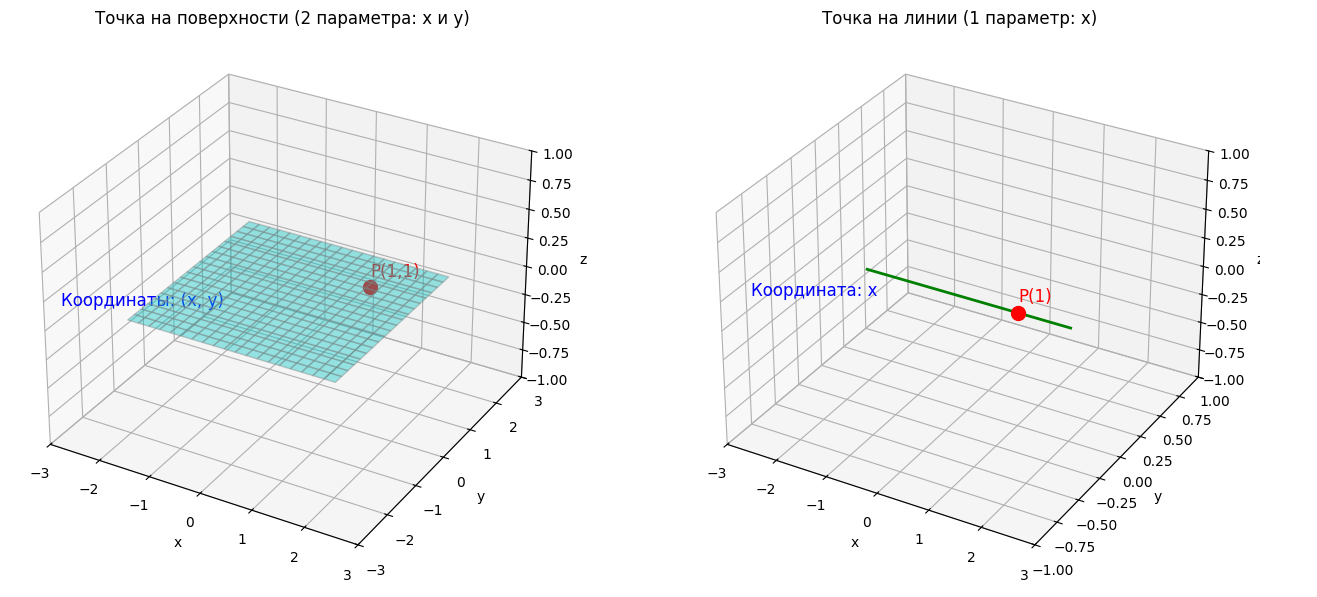
\includegraphics[scale=0.4]{images/img12}
	$$
	Если на систему материальных точек действуют активные силы $F_i(X_i, Y_i, Z_i)$, $i = 1, 2, \dots, n$, то как декартовы, так и обобщённые координаты точек будут изменяться с течением времени, т.~е. будут функциями временного аргумента $t$:
	\begin{equation}
		\label{4.16}
		x_i = x_i(t), \quad y_i = y_i(t), \quad z_i = z_i(t), \quad i = 1, 2, \dots, n,
		\quad q_s = q_s(t), \quad s = 1, 2, \dots, k.
	\end{equation}
	Функции \eqref{4.16} зависят от приложенных к системе активных сил, т.~е. определяются неоднозначно. Чтобы подчеркнуть это обстоятельство, мы будем обозначать их дифференциалы через $\delta x_i$, $\delta y_i$, $\delta z_i$, $\delta q_s$, $i = 1, 2, \dots, n$, $s = 1, 2, \dots, k$. 
	\begin{itemize}
		\item Величины $\delta x_i$, $\delta y_i$, $\delta z_i$ обозначают возможные перемещения системы материальных точек.
		\item Величины $\delta q_s$, $s = 1, 2, \dots, k$, называют \textit{вариациями обобщённых координат}.
	\end{itemize} 
	Заметим, что поскольку обобщённые координаты не стеснены никакими ограничениями, то их вариации произвольны и независимы.
	\\\\
	Тогда дифференциалы функций \eqref{4.16} в силу \eqref{4.15} связаны соотношениями
	\begin{equation}
		\label{4.18}
		\delta x_i = \sum_{s=1}^k \frac{\partial x_i}{\partial q_s} \delta q_s, \quad
		\delta y_i = \sum_{s=1}^k \frac{\partial y_i}{\partial q_s} \delta q_s, \quad
		\delta z_i = \sum_{s=1}^k \frac{\partial z_i}{\partial q_s} \delta q_s, \quad
		i = 1, 2, \dots, n.	
	\end{equation}
	Подставим выражения для возможных перемещений \eqref{4.18} в общее уравнение динамики. Изменив знак и порядок суммирования, имеем
	\begin{equation}
		\label{4.19}
		\sum_{s=1}^k \delta q_s 
		\left[
		\sum_{i=1}^n m_i 
		\left(
		\frac{d^2 x_i}{dt^2} \frac{\partial x_i}{\partial q_s} + 
		\frac{d^2 y_i}{dt^2} \frac{\partial y_i}{\partial q_s} + 
		\frac{d^2 z_i}{dt^2} \frac{\partial z_i}{\partial q_s}
		\right) 
		- 
		\sum_{i=1}^n 
		\left(
		X_i \frac{\partial x_i}{\partial q_s} + 
		Y_i \frac{\partial y_i}{\partial q_s} + 
		Z_i \frac{\partial z_i}{\partial q_s}
		\right)
		\right] = 0.
	\end{equation}
	Обозначим
	\begin{equation}
		\label{4.20}
		Q_s = \sum_{i=1}^n 
		\left(
		X_i \frac{\partial x_i}{\partial q_s} + 
		Y_i \frac{\partial y_i}{\partial q_s} + 
		Z_i \frac{\partial z_i}{\partial q_s}
		\right), \quad s = 1, 2, \dots, k.
	\end{equation}
	Величину $Q_s$ называют \textbf{обобщённой силой}, отнесённой к координате $q_s$. 
	\\\\
	Смысл обобщённых сил можно прояснить, рассматривая возможную работу $\delta A$ всех активных сил, действующих на систему на её произвольном возможном перемещении:
	\begin{equation*}
		\delta A = \sum_{i=1}^n 
		\left(
		X_i \delta x_i + Y_i \delta y_i + Z_i \delta z_i
		\right),
	\end{equation*}
	которую в силу \eqref{4.18} можно записать следующим образом:
	\begin{equation*}
		\delta A = \sum_{s=1}^k 
		\left[
		\sum_{i=1}^n 
		\left(
		X_i \frac{\partial x_i}{\partial q_s} + 
		Y_i \frac{\partial y_i}{\partial q_s} + 
		Z_i \frac{\partial z_i}{\partial q_s}
		\right)
		\right] \delta q_s,
	\end{equation*}
	или
	\begin{equation*}
		\delta A = \sum_{s=1}^k Q_s \delta q_s.
	\end{equation*}
	Если рассмотреть такое возможное перемещение системы, при котором среди обобщённых координат изменяется только координата $q_s$, то $\delta A = Q_s \delta q_s$, откуда получаем
	\begin{equation*}
		Q_s = \frac{\delta A}{\delta q_s}, \quad s = 1, 2, \dots, k.
	\end{equation*}
	Если система материальных точек представляет собой твёрдое тело, то сумма элементарных работ всех внутренних активных сил на любом возможном перемещении системы равна нулю. По этой причине в данном случае при вычислении обобщённых сил достаточно учесть только внешние активные силы, действующие на систему.
	\\\\
	Величина
	\begin{equation*}
		T = \sum_{i=1}^n \frac{m_i v_i^2}{2} = \sum_{i=1}^n \frac{m_i}{2} \left( \dot{x}_i^2 + \dot{y}_i^2 + \dot{z}_i^2 \right)
	\end{equation*}
	есть \textbf{кинетическая энергия системы материальных точек}.
	\\\\
	Уравнения 
	\begin{equation}
		\label{4.26}
		\frac{d}{dt} \frac{\partial T}{\partial \dot{q}_s} - \frac{\partial T}{\partial q_s} = Q_s, \quad s = 1, 2, \dots, k.
	\end{equation}
	были впервые получены Лагранжем и называются \textbf{уравнениями Лагранжа второго рода}. Это дифференциальные уравнения второго порядка относительно обобщённых координат. Их число равно числу степеней свободы системы материальных точек.
	\\\\
	Допустим, что действующая на материальную точку сила $\vec{F}$ зависит только от положения точки, т. е.
	\[
	X = X(x, y, z), \quad Y = Y(x, y, z), \quad Z = Z(x, y, z).
	\]
	Область определения функций $X$, $Y$, $Z$ называется \textbf{силовым полем}. Если движение точки происходит в силовом поле и работа силы $\vec{F}$
	\[
	dW = Xdx + Ydy + Zdz
	\]
	не зависит от пути, по которому происходит перемещение точки, а зависит лишь от начального $M_1$ и конечного $M_2$ положений точки, то такое поле называется \textbf{потенциальным}, а сила $\vec{F}$ --- \textbf{консервативной}. Примеры консервативных сил: \begin{itemize}
		\item сила тяготения;
		\item сила упругости пружины, подчиненная закону Гука
		\item сила тяжести.
	\end{itemize}
	В потенциальном силовом поле работа по любому замкнутому контуру равна нулю. Это условие, как доказывается в теории криволинейных интегралов, эквивалентно тому, что элементарная работа силы $\vec{F}$ есть полный дифференциал некоторой функции $U(x, y, z)$:
	\[
	dW = \frac{\partial U}{\partial x}dx + \frac{\partial U}{\partial y}dy + \frac{\partial U}{\partial z}dz.
	\]
	Функция $U(x, y, z)$ называется \textbf{силовой функцией}. Поскольку, с другой стороны, по определению полного дифференциала
	\[
	\frac{\partial U}{\partial x}dx + \frac{\partial U}{\partial y}dy + \frac{\partial U}{\partial z}dz,
	\]
	то
	\begin{equation}
		\label{3.10}
		X = \frac{\partial U}{\partial x}, \quad Y = \frac{\partial U}{\partial y}, \quad Z = \frac{\partial U}{\partial z}. 
	\end{equation}
	Существование гладкой функции $U$, удовлетворяющей соотношениям \eqref{3.10}, является необходимым и достаточным условием для того, чтобы силовое поле было потенциальным. 
	\\\\
	По теореме об изменении кинетической энергии системы
	\begin{equation}
		\label{4.10}
		dT = \sum_{i=1}^{m}(X_i dx_i + Y_i dy_i + Z_idz_i).
	\end{equation}
	Пусть все активные силы, действующие на точки системы, являются консервативными и $U_i(x, y, z)$, $i = 1, 2, \ldots, n$, — силовая функция силы $\vec{F}_i(X_i, Y_i, Z_i)$. 
	Функцию
	\[
	U(x_1, y_1, z_1, \ldots, x_n, y_n, z_n) = \sum_{i=1}^{n} U_i(x_i, y_i, z_i)
	\]
	называют \textbf{силовой функцией системы материальных точек}. Очевидно, она удовлетворяет условиям
	\begin{equation}
		\label{4.11}
		X_i = \frac{\partial U}{\partial x_i}, \quad Y_i = \frac{\partial U}{\partial y_i}, \quad Z_i = \frac{\partial U}{\partial z_i}, \quad i = 1, 2, \ldots, n. 
	\end{equation}
	Функция, противоположная по знаку силовой функции,
	\[
	V = -U
	\]
	есть \textbf{потенциальная энергия системы материальных точек}. Обе эти функции определены с точностью до аддитивной постоянной.
	\\\\
	Подставив \eqref{4.11} в \eqref{4.10}, получим
	\begin{equation}
		\label{4.12}
		dT = \sum_{i=1}^{n} \left( \frac{\partial U}{\partial x_i} dx_i + \frac{\partial U}{\partial y_i} dy_i + \frac{\partial U}{\partial z_i} dz_i \right) = dU,
	\end{equation}
	где $dU$ — полный дифференциал силовой функции.
	\\\\
	Величина $T + V$ есть \textbf{полная механическая энергия системы материальных точек}. Из равенства \eqref{4.12} следует $d(T + V) = 0$, или $T + V = \text{const}$. Таким образом, полная механическая энергия системы материальных точек, находящихся под действием консервативных сил, есть величина постоянная.
	\\\\
	Пусть активные силы, действующие на точки системы, являются консервативными. В этом случае существует скалярная функция $U(x_1, y_1, z_1, \dots, x_n, y_n, z_n)$, удовлетворяющая условиям
	\begin{equation*}
		X_i = -\frac{\partial U}{\partial x_i}, \quad Y_i = -\frac{\partial U}{\partial y_i}, \quad Z_i = -\frac{\partial U}{\partial z_i}.
	\end{equation*}
	Тогда обобщённые силы могут быть представлены в виде
	\begin{equation*}
		Q_s = \sum_{i=1}^n \left( 
		X_i \frac{\partial x_i}{\partial q_s} + 
		Y_i \frac{\partial y_i}{\partial q_s} + 
		Z_i \frac{\partial z_i}{\partial q_s} 
		\right) = -\frac{\partial U}{\partial q_s}.
	\end{equation*}
	Соответственно, уравнения Лагранжа можно записать следующим образом:
	\begin{equation}
		\label{4.27}
		\frac{d}{dt} \frac{\partial T}{\partial \dot{q}_s} - \frac{\partial T}{\partial q_s} + \frac{\partial U}{\partial q_s} = 0, \quad s = 1, 2, \dots, k.
	\end{equation}
	Если ввести функцию Лагранжа, или \textbf{кинетический потенциал системы материальных точек}, как $L = T - U$ (где $T$~--- полная кинетическая энергия), то уравнения \eqref{4.27} запишутся следующим образом:
	\begin{equation}
		\label{4.28}
		\frac{d}{dt} \left( \frac{\partial L}{\partial \dot{q}_s} \right) - \frac{\partial L}{\partial q_s} = 0, \quad s = 1, 2, \ldots, k,
	\end{equation}
	поскольку очевидно, что
	\[
	\frac{\partial U}{\partial \dot{q}_s} = 0, \quad s = 1, 2, \ldots, k.
	\]
	Уравнения \eqref{4.28} представляют собой \textbf{уравнения Лагранжа второго рода для консервативных сил}.
	Если система материальных точек представляет собой твёрдое тело, то уравнения Лагранжа можно записать в этой форме, если консервативными являются только внешние активные силы.
	
	\section{Модели и моделирование, их определение и роль}
	\textbf{Математическая модель} - любая структура математических символов, определенным образом организованная с соответствующими связями между элементами структуры, подчиняющимися законам математической логики. 
	Математическая модель всегда соответствует исходному изучаемому\textbf{ объекту реальности}, а \textbf{частям объекта и их функциональным свойствам} - символы и связи математической структуры, которые соответствующим образом интерпретируются, т.е. наделяются физическим смыслом.
	\\\\
	\textbf{Математическое моделирование} - это процесс, предполагающий динамику организованных действий исследователя, направленных на сопоставление изучаемому объекту реальности конкретной математической модели или класса моделей.
	\\\\
	Моделирование включает: 
	\begin{itemize}
		\item процесс построения модели, 
		\item исследование модели,
		\item извлечение новой информации об объекте реальности с помощью разработанной модели.
	\end{itemize}
	Классификация моделей может быть представлена следующей таблицей
	$$
	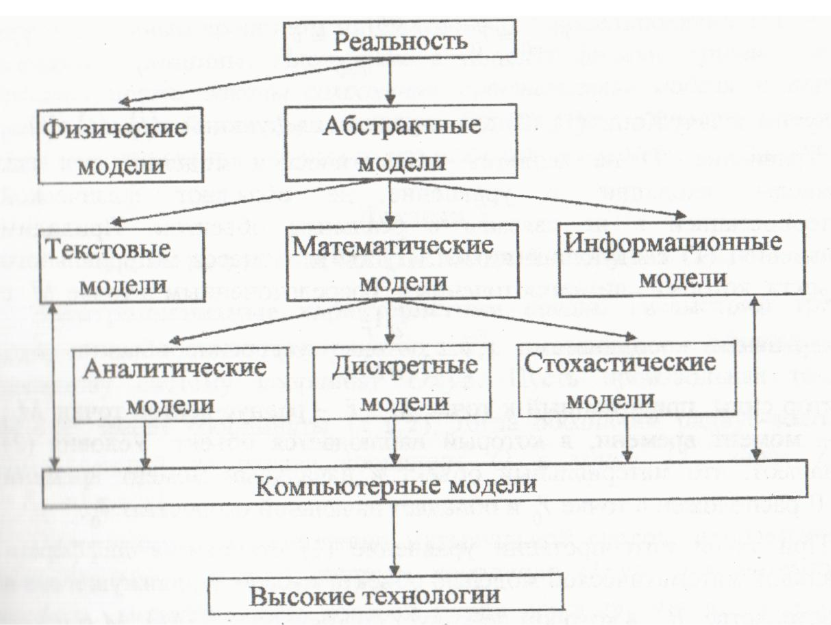
\includegraphics[width=0.5\linewidth]{images/img24.png}
	$$
	\begin{itemize}
		\item \textbf{Физическая модель} - это упрощенный физический объект, заменяющий реальный изучаемый объект, который в лабораторных условиях экспериментально исследуется с целью выявления закономерностей исходного объекта реальности.
		\item \textbf{Текстовые модели} являются описательными, выполненными на естественном языке исследователя. 
		\item \textbf{Математические модели} основываются на использовании специальных математических символов, терминов и понятий, из которых конструируется модель. Например, число, функция, график, уравнение, производная, алгебраические и булевы операции, алгоритм, программа и другие структуры, которые в каждой конкретной математической модели имеют свою физическую интерпретацию.
		\item \textbf{Информационные модели} базируются на сборе информации об изучаемом физическом объекте, на кодировании и хранении информации, на ее систематизации и переработке определенными методами с целью получения новой информации об объекте. Например, базы данных деталей и материалов, используемых в производстве автомобилей, могут рассматриваться как информационные модели автомобиля.
		\item Для \textbf{аналитических моделей} характерно применение функциональных, дифференциальных, интегральных и других соотношений и уравнений для описания изучаемого объекта с использованием методов непрерывной математики. 
		\item \textbf{Дискретные модели}, как правило, основываются на использовании алгоритмов дискретной математики, формальной логики и вычислительных процедур для исследовании параметров объекта. 
		\item \textbf{Стохастические модели} используются, когда параметры объекта испытывают многочисленные внутренние и внешние влияния, не подчиняются детерминированным закономерностям и рассматриваются как случайные величины.
		\item \textbf{Высокие технологии} представляют собой сочетание математических, информационных и компьютерных моделей. Основным признаком высоких технологий является информационное взаимодействие модели с моделируемым объектом в реальном режиме времени с использованием датчиков, измерительной техники и линий связи, поставляющих информацию с функционирующего объекта.
	\end{itemize}
	\textbf{Классификация моделей по применяемому математическому аппарату}: алгебраические, дифференциальные, интегральные, стохастические, вероятностные, дискретные, логические и др.
	\\\\
	\textbf{Классификация моделей по отраслям науки}: модели в физике,
	биологии, социологии, химии, модели в медицине и технике, модели в
	экономике и др.
	\\\\
	\textbf{Физический объект $A$} -- это ситуация, явление, процесс, материальный объект и др., являющиеся фрагментами реальности. При изучении объекта $A$ выделяют его основные свойства $\vec{S} = (S_1, S_2, \ldots, S_N)$.  
	\\\\
	Физическому объекту $A$ ставится в соответствие идеальный объект $A'$, называемый \textbf{математической моделью} объекта $A$ относительно совокупности свойств $\vec{S}$. В связи с этим объекту $A$ могут быть сопоставлены различные модели $A'$ в зависимости от свойств объекта $A$, положенных в основу модели. В результате строится ряд математических моделей $A_1', A_2', \ldots$, всесторонне описывающих изучаемый объект $A$. При этом учитывается принцип \textbf{взаимной дополняемости моделей} и принцип \textbf{иерархии моделей}.  
	\\\\
	Таким образом, математические модели обладают свойством \textbf{множественности}, то есть для каждого физического объекта могут быть построены различные \textbf{неравносильные модели}.  
	\\\\
	Второе свойство математических моделей -- это свойство \textbf{универсальности}, когда одна и та же модель может описывать \textbf{принципиально} различные физические объекты.
	\\\\
	\textbf{Основные этапы моделирования.} Любой процесс моделирования, вне зависимости от предметной области, можно разбить на две основные части:
	\begin{enumerate}
		\item построение   математической   модели, соответствующей конкретному физическому объекту;
		\begin{enumerate}
			\item \textbf{Качественное исследование физического объекта $A$.} Свoдится к выделению основных параметров, элементов, связей объекта ($\vec{S} \text{ -- свойства}$), подлежащих моделированию. При этом на основании экспериментальных данных отбрасываются несущественные факторы, слабо влияющие на функционирование объекта $A$ в пределах, требуемых изменением параметров.
			\item \textbf{Построение содержательной модели.} Выбирается одна из предметных областей: физическая, механическая, биологическая, химическая, экономическая и т. д. При построении содержательной модели формулируются соответствующие гипотезы, постулаты, законы, которые ложатся в основу математической модели. Используется, как правило, устоявшаяся информация об объекте и универсальные законы природы.
			\item \textbf{Построение математической модели $A'$.} Содержательная модель объекта описывается на формальном математическом языке. При этом каждому реальному элементу, свойству объекта $А$ соответствует элемент математической модели, то есть символ, наделенный физическим смыслом. При построении математической модели, как правило, используются хорошо разработанные математические теории: дифференциальное и интегральное исчисление, дискретная математика, линейная  алгебра, теория вероятностей и др.
		\end{enumerate}
		\item практическое использование разработанной математической модели.
		\begin{enumerate}
			\item \textbf{Постановка математических задач и их решение.} На
			практике обычно отдельные параметры объекта известны или легко
			могут быть определены экспериментально. При использовании математической
			модели возникают математические задачи, которые должны быть
			решены в рамках исходной модели. В случае дифференциальных
			моделей задачи, как правило, ставятся в форме краевых или начально-краевых задач. Сформулированная задача также может быть рассмотрена как математическая модель одной из сторон физического объекта.
			\item \textbf{Истолкование результатов моделирования. Верификация модели.} Результаты решения задач, поставленных на основании математической модели, должны быть отождествлены со значениями реальных параметров физического объекта и определена точность моделирования, то есть возникает \textbf{проблема верификации}. 
			\\\\
			\textbf{Верификация модели} - система мероприятий по определению
			адекватности модели физическому объекту. Если используемая модель достаточно апробирована на практике, то верификация не проводится. Если же рассматривается модель с неапробированными значениями параметров или новая модель, то верификация сводится к следующему: к сравнению результатов моделирования с экспериментальными данными, к сравнению с выводами, полученными на основании других моделей, к более глубокому теоретическому исследованию и обоснованию модели.
			
		\end{enumerate}
	\end{enumerate}
	\textbf{Основные цели математического моделирования}.
	\begin{itemize}
		\item Модель необходима для изучения внутренней структуры объекта и взаимодействия между его элементами, для выявления его новых свойств и характера связей с окружающей реальностью.
		\item Модель необходима для управления объектом или процессом при заданных целях и критериях.
		\item Модель необходима для прогнозирования поведения объекта в будущем при различных начальных режимах.
	\end{itemize}
	\textbf{Вычислительный эксперимент} – многократное численное решение математических задач в пределах определённой математической модели при различных исходных данных с применением вычислительной техники для выявления новых закономерностей изучаемого объекта. 
	\\\\
	Типичные математические модели, соответствующие естественнонаучным процессам (явлениям, объектам), формулируются в виде уравнений математической физики. Большинство реальных процессов описывается нелинейными уравнениями и лишь в первом приближении (при малых значениях параметров, малых отклонениях от положения равновесия и т.п.) эти уравнения можно заменить линейными. Естественно, такие задачи, как правило, мы не умеем решать аналитически. Поэтому построение численного эксперимента предназначено для «дискретизации» математической модели, т.е. для перехода к системе алгебраических уравнений и описания алгоритмов ее решения.
	$$
	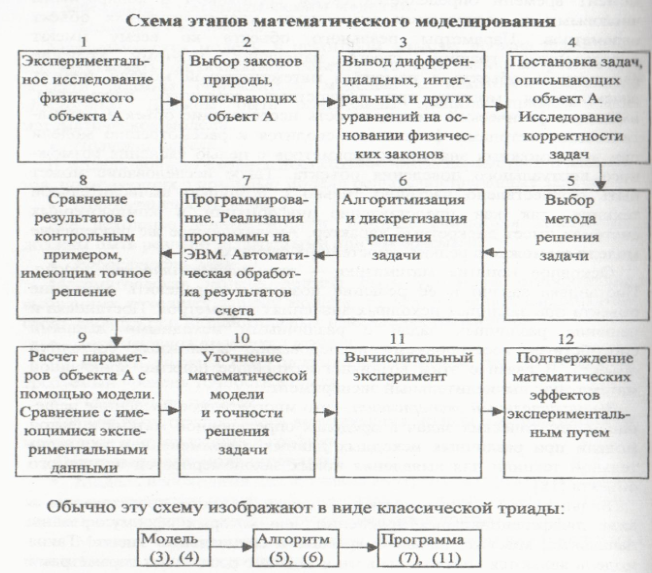
\includegraphics[width=0.5\linewidth]{images/img25.png}
	$$
	\textbf{Требования к математическим моделям}.
	\begin{itemize}
		\item \textbf{Адекватность модели.} Математическая модель, в некотором смысле, должна правильно соответствовать физическому объекту, то есть свойства реального объекта должны описываться моделью с некоторой разумной точностью. Должны быть определены границы применимости математической модели.
		\item \textbf{Полнота модели.} В модель должно входить достаточное число параметров и элементов, позволяющих с помощью модели решать поставленные задачи
		\item \textbf{Продуктивность модели.} Все исходные данные модели, которые считаются заданными, должны быть реально задаваемыми или измеряемыми.
		\item \textbf{Устойчивость модели.} Математическая модель должна быть устойчива относительно выбранных исходных данных модели, т.е. не менять кардинально своих свойств при незначительных изменениях параметров.
		\item \textbf{Достаточная простота модели.} Из модели должны быть исключены элементы, не влияющие им требуемый уровень точности модели.
		\item \textbf{Наглядность модели.} Должна быть осуществлена визуализация модели с использованием мониторов и компьютерной графики.
		
	\end{itemize}
	
	\section{Постановка краевых задач в задачах моделирования (в физике и биологии)}
	\textbf{Задача электростатики для диэлектрического прозрачного тела}. Рассмотрим однородное диэлектрическое тело $D_1$ с диэлектрической проницаемостью $\varepsilon_1$. Внешняя область $D_2$ заполнена однородной средой (например, воздухом) с диэлектрической проницаемостью $\varepsilon_2$. Во внешней области $D_2$ расположен источник электрического поля $D_0$, который порождает \textbf{первичное электрическое поле} с потенциалом $u_0$. При взаимодействии поля $u_0$ с границей тела $\Gamma$ в области $D_2$ образуется отражённое поле $u'$, а в области $D_1$ проникает поле $u_1$. Обозначим через $u_2 = u_0 + u'$~--- суммарное поле в $D_2$.
    $$   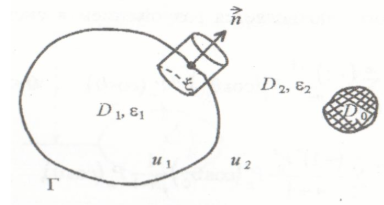
\includegraphics[width=0.5\linewidth]{images/img37.png}
    $$
\textbf{Краевая задача 1}
\begin{equation}
\label{cr-1}
    \begin{cases}
    \Delta u_1 = 0\ \text{в}\ D_1,\\
    \Delta u_2 = 0\ \text{в}\ D_2,\\
    u_1|_\Gamma = u_2|_\Gamma, \\
    \varepsilon_1 \left. \dfrac{\partial u_1}{\partial \nu} \right|_\Gamma = \varepsilon_2 \left. \dfrac{\partial u_2}{\partial \nu} \right|_\Gamma,\\
    u_2(M) = 0\ \text{при}\ M \rightarrow \infty
\end{cases}
\end{equation}
В задаче \eqref{cr-1} функция $u_0$
считается заданной в области $D_2$, параметры $\epsilon_1, \epsilon_@$
определены, геометрия граничной области
$\Gamma$
известна. Требуется найти неизвестную функцию $u_1$
в области $D_1$
и неизвестную функцию $u_2$
в области $D_2$, которые удовлетворяют граничным
условиям.
\\\\
\textbf{Задача электростатики для металлического тела.}
Рассмотрим металлическое тело $D_1$ с внешней областью $D_2$, заполненной средой с диэлектрической проницаемостью $\varepsilon_2$. Пусть первичное поле $u_0$ взаимодействует с граничной поверхностью $\Gamma$, на которой поддерживается заданный потенциал $C = \text{const}$, т.е. выполнено граничное условие для суммарного потенциала $u = u_0 + u'$, где $u'$~--- отражённое поле в области $D_2$. Сформулируем соответствующую задачу.
\\\\
\textbf{Краевая задача 2 (внешняя задача Дирихле)}
\begin{equation}
\begin{cases}
    \Delta u' = 0\ \text{в}\ D_2, \\ (u' + u_0)|_\Gamma = C, \\ u'(M) \rightrightarrows 0\ \text{при}\ M \rightarrow \infty
\end{cases}
\end{equation}
Рассмотрим также случай, когда на поверхности $\Gamma$ металлического тела $D_1$ распределены заряды с заданной поверхностной плотностью $\sigma$, тогда взаимодействие первичного поля $u_0$ с поверхностью $\Gamma$ определяется граничным условием.
\\\\
\textbf{Краевая задача 3 (внешняя задача Неймана)}
\begin{equation}
    \begin{cases}
        \Delta u' = 0\ \text{в}\ D_2, \\ \left. \dfrac{\partial (u' + u_0)}{\partial \nu} \right|_\Gamma = -4\pi \sigma, \\ u'(M) \rightrightarrows 0\ \text{при}\ M \rightarrow \infty
    \end{cases}
\end{equation}
Пусть популяция размещается в области \(D \subset \mathbb{R}^3\), которая называется \textbf{областью популяции}. Будем считать, что поток вещества \(X\) через границу \(\Gamma = \partial D\) равен нулю, то есть выполняется условие \(\dfrac{\partial \rho}{\partial \vec{n}} \bigg|_{\Gamma} = 0\). Отсюда следует, что поток через \(\Gamma\) также равен нулю. Потребуем, чтобы потоки не пересекали границу \(\Gamma\), то есть дополнительно положим поток равным нулю \(\left( \dfrac{\partial u}{\partial \vec{n}} \bigg|_{\Gamma} = 0 \right)\). Поставим задачу.
\\\\
\textbf{Вторая смешанная краевая задача.}
\begin{equation}
\label{cr-3}
    \begin{cases}
        \dfrac{\partial u}{\partial t} = \operatorname{div} (\mu \nabla u-\nu u\nabla \rho)+(\alpha - \gamma u) u \equiv L_1(u,\rho),\quad \text{в} \quad D \times (0 < t < \infty),\\
        \dfrac{\partial \rho}{\partial t} =\operatorname{div} (\nu \rho)+\delta u-\beta \rho= L_2(u, \rho) \quad \text{в} \quad D \times (0 < t < \infty),\\
        \dfrac{\partial u(M, t)}{\partial \vec{n}} \bigg|_{M \in \Gamma} = 0, \quad t \geq 0,\\ 
        \dfrac{\partial \rho(M, t)}{\partial \vec{n}} \bigg|_{M \in \Gamma} = 0, \quad t \geq 0,\\
        u(M,t)\big|_{t=0} = \varphi(M), \quad M \in \overline{D}, 
        \\ \rho(M,t)\big|_{t=0} = \psi(M), \quad M \in \overline{D},
    \end{cases}
\end{equation}
где \( \varphi(M) \) --- начальная плотность амёб в \(D\), \( \psi(M) \) --- начальная плотность химического вещества в \(D\).
\\\\
Замена граничных условий второго рода на граничные условия первого рода
\[
u\big|_{\Gamma} = 0,\quad \rho\big|_{\Gamma} = 0,
\]
приведет к \textbf{первой смешанной краевой задачу}.
\\\\
Очевидно, что для существования популяции важна ситуация, когда она находится в некотором стабильном положении, слабо изменяющемся во времени. Предположим, что существуют некоторые начальные функции
\[
\varphi = u_0(M), \quad \rho = \rho_0(M), \quad \psi = \psi_0(M), \quad M \in D,
\]
такие, что решение задачи \eqref{cr-3} не зависит от времени \(t\), то есть
\[
\frac{\partial u}{\partial t} = 0, \quad \frac{\partial \rho}{\partial t} = 0.
\]
В результате для определения стационарных решений \(u = u_0(M), \rho = \rho_0(M)\) получим следующую задачу\\\\
\textbf{Краевая адача Неймана}
\begin{equation}
    \begin{cases}
        L_1(u, \rho) = 0,\ L_2(u, \rho) = 0 \quad \text{в} \quad D,\\
        \left. \dfrac{\partial u}{\partial n} \right|_{\Gamma} = 0, \\ 
        \left. \dfrac{\partial \rho}{\partial n} \right|_{\Gamma} = 0.
    \end{cases}
\end{equation}
По краевой мере два решения этой задачи существуют:
\begin{equation}
\nu_0 = \dfrac{\alpha}{\gamma} - \text{const}, \quad 
\rho_0 = \dfrac{\alpha \delta}{\beta \gamma} - \text{const}; \quad 
u_0 = 0, \quad \rho_0 = 0.
\end{equation}
Из всех стационарных решений начально-краевой задачи для уравнений популяции выделяют решения, которые устойчивы относительно начальных возмущений.
Рассматриваем задачу \eqref{cr-3} при возмущённых начальных функциях 
\[
\psi = u_0(M) + \epsilon_1(M), \quad 
\rho_0(M) + \epsilon_2(M),
\]
где \(\epsilon_1, \epsilon_2\) --- достаточно малые величины. Если решение задачи \eqref{cr-3} с возмущёнными начальными условиями стремится к стационарному решению, то есть
\[
u(M, t) \rightarrow u_0(M), \quad 
\rho(M, t) \rightarrow \rho_0(M) \quad \text{при} \quad t \rightarrow 0,
\]
то стационарное решение \(u_0, \rho_0\) называется \textbf{диссипативной структурой}. Для однокомпонентной популяции с выпуклым ареалом \(D\) такие структуры не существуют.
\\\\
\textbf{Описательная модель.} Рассмотрим популяцию леммингов.
Модель строится с учетом свойств отдельной особи и взаимодействия её с различными факторами внутри популяции и в окружающей среде. В модель включены две компоненты: потребитель-лемминг и ресурс-растительность.  Пространственные аспекты учитываются существенно. При этом используются \textbf{клеточные автоматы}, являющиеся одним из средств моделирования малочисленных популяций.
\\\\
Модель функционирует следующим образом.
\begin{itemize}
    \item Участок тундры, заселенный популяцией, \textit{разбивается на клетки}. В результате получаем прямоугольную таблицу.
    \item  Состояние каждой клетки таблицы описывается \textit{значением ресурса} (пиши) в клетке и \textit{списком потребителей} (леммингов, находящихся (проживающих) в клетке).
    \item  Каждый потребитель описывается \textit{набором свойств}: возраст, жизненный потенциал и способность к размножению.
    \item В клетке, в которой находится потребитель (лемминг), он потребляет некоторый ресурс. Если потребляемый ресурс больше некоторого значения, то \textit{жизненный потенциал} потребителя увеличивается, в противном случае потенциал уменьшается, но не может стать отрицательным. Если жизненный потенциал падает до некоторого минимального уровня - потребитель гибнет.
    (Жизненный потенциал не может увеличиваться безгранично, увеличивается до некоторого порогового значения, имеющего смысл максимальной жизнестойкости потребителя в зависимости от возраста).
    \item Между потребителями существует конкуренция за обладание ресурсами, поэтому увеличение плотности популяции приводит к снижению жизнестойкости. Если два потребителя находятся в одной клетке, жизненный потенциал уменьшается.
    \item На каждой итерации значение способности к размножению увеличивается и зависит от жизненного потенциала. Более жизнестойкие потребители быстрее наращивают способность к произведению потомства. Когда способность к размножению увеличивается до некоторого порогового значения, появляется потомство. При этом значение способности к размножению полагается равным нулю и процесс повторяется.
    \item На каждой итерации происходит перемещение потребителей. Эти перемещения происходят с учетом благоприятности условий обитания в клетке. Степень благоприятности описывается штрафом, который начисляется в зависимости от плотности популяции в клетке и количества растительности в клетке.
    \item Если возраст потребителя меньше некоторого значения, он не передвигается, не потребляет ресурс, не участвует в столкновениях и не размножается. 
Для леммингов — это возрастание достижения половой зрелости.
Таким образом, вводятся две категории потребителей: половозрелых и неполовозрелых. Число половозрелых учитывается в плотности популяции.
\end{itemize}
$$
    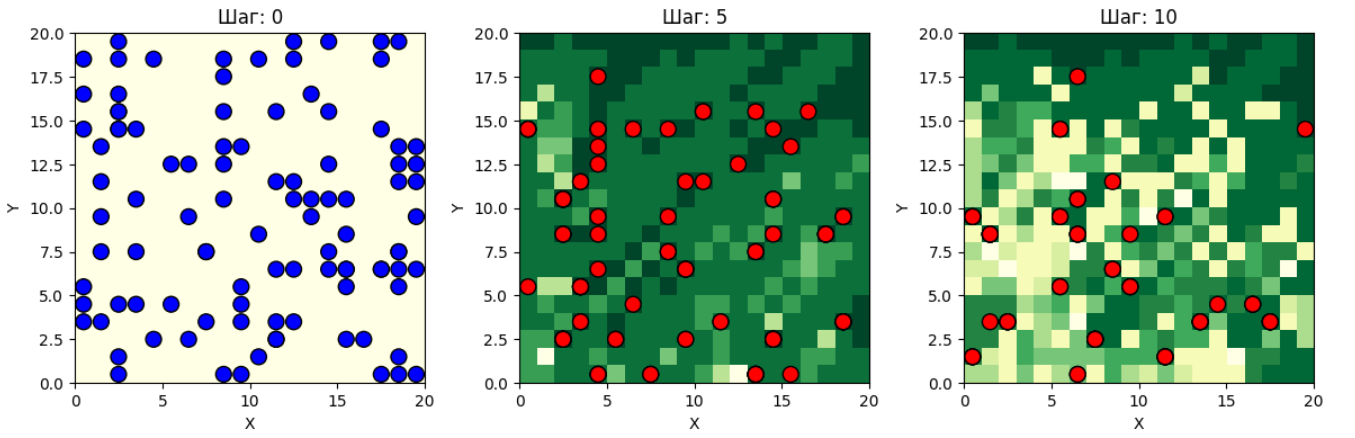
\includegraphics[width=0.7\linewidth]{images/img38.png}
$$
\textbf{Состояние системы}, рассматриваемой как единое целое, определяется некоторыми основными функциями
$
u_1, u_2, \ldots, u_n,
$
которые представляются как \( n \)-мерный вектор
$
\vec{u} = (u_1, u_2, \ldots, u_n).
$
В качестве примера сложной системы можно рассмотреть \( n \) взаимодействующих популяций живых организмов, где \( u_i \) --- численность \( i \)-ой популяции или плотность пространственного распределения особей \( i \)-ого сорта. В последнем случае функции \( u_i \) зависят от пространственных переменных 
$
\vec{r} = (x, y, z).
$
Естественно, вектор-функция \( \vec{u} \) изменяется с течением времени, поэтому является также функцией времени \( t \). Любая система всегда подвергается воздействию внешних факторов. Выделим наиболее существенные параметры, характеризующие внешнюю среду и влияющие на изучаемую систему. Совокупность числовых и функциональных параметров среды обозначим вектором $\vec{\tau} = (\tau_1, \tau_2, \ldots, \tau_N)$.
Параметры среды могут эволюционировать по некоторым детерминированным известным законам, которые в простейшем случае описываются системой обыкновенных дифференциальных уравнений
\begin{equation}
\frac{d\vec{\tau}}{dt} = f(\vec{\tau}, t).
\end{equation}
В случае, когда число внешних параметров велико, параметры 
не поддаются аналитическому описанию, быстро осциллируют и имеют непредсказуемый характер, для моделирования их воздействия на систему вводится вектор случайных величин
$
\vec{\xi} = (\xi_1, \xi_2, \ldots, \xi_5).
$
Случайные величины отвечают за неуправляемость эволюционных процессов.
Сообщество популяций характеризуется также и своими внутренними параметрами
$
\lambda = (\lambda_1, \lambda_2, \ldots, \lambda_C),
$
которые называются \textbf{свойствами системы}. В число этих параметров входят индивидуальные свойства особей: возраст, масса, цвет, пол особей и другие.
	Состояние исследуемого объекта определяется вектор-функцией
\begin{equation}
  \vec{u} = \vec{u}(t, \vec{r}, \vec{\lambda}, \tau, \vec{\xi}). \tag{2.98}
\end{equation}
Поскольку указанная вектор-функция может зависеть от некоторых параметров управления
$
\vec{v} = (v_1, v_2, \ldots, v_m),
$
которые определяют воздействие человека на систему, для получения уравнения, описывающего эволюцию состояния, вычисляется её производная
\begin{equation}
  \frac{d\vec{u}}{dt},
\end{equation}
и представляется в виде \textbf{эволюционного уравнения}
\begin{equation}
  \frac{d\vec{u}}{dt} = \Phi(\vec{u}),
\end{equation}
где эволюционный оператор $\Phi$ имеет самую общую структуру и может быть функциональным, дифференциальным, интегральным, конечномерным и т.д.
	\chapter{Численные методы}
	\section{Численные методы решения нелинейных уравнений, систем и задач оптимизации}
	Пусть задана функция $f(x)$ действительного переменного $x \in \mathbb R$. Требуется найти корни уравнения 
	\begin{equation}
		\label{nle-1}
		f(x) = 0,
	\end{equation}
	или, что то же самое, нули функции $f(x)$. 
	\begin{theorem}
		Если функция $f(x)$ непрерывна на отрезке $[a,b]$ и принимает на его концах значения разных знаков, то на этом отрезке существует по крайней мере один корень уравнения $f(x) = 0$.
		Если при этом функция $f(x)$ будет монотонной на отрезке $[a,b]$, то она может иметь только один корень.
	\end{theorem}
	\noindent
	То есть мы определили условия, при которых задача будет корректно поставленной.
	Задача нахождения корней уравнения \eqref{nle-1} обычно решается в два этапа:
	\begin{enumerate}
		\item \textbf{Отделение корней.}\\\\
		На этом этапе изучается расположение корней (в общем случае на комплексной плоскости), проводится их разделение, то есть выделяются области, содержащие только один корень. Кроме того изучается вопрос о кратности корней. Находятся некоторые начальные приближения $x^0$ для точного решения.
		
		\item \textbf{Построение метода.}
		\\\\
		На этом этапе, используя заданное начальное приближение, строится итерационный процесс, позволяющий уточнить значение отыскиваемого корня до некоторой заданной точности $\varepsilon$. То есть, зная начальное приближение $x^0$, мы строим последовательность $x^k \xrightarrow[k\to\infty]{\varepsilon}x^*$.
	\end{enumerate}
	Применение \textbf{метода простой итерации} требует предварительного приведения уравнения $f(x) = 0$ к каноническому виду 
	\begin{equation}
		\label{mpi-1}
		x = \varphi(x),
	\end{equation} где $\varphi(x)$ --- это заданная функция. Для канонической формы метод простой итерации будет иметь следующий вид: 
	\begin{equation}
		\label{mpi-2}
		x^{k+1} = \varphi(x^k),\ k = 0,1,2,\ldots,
	\end{equation}
	где $x^k$ --- последовательность, начинающаяся с $x^0$, которая должна сходится к точному решению.
	\\\\
	Для построения сходящегося метода простой итерации в практических вычислениях проверяется \textbf{достаточное условие сходимости}: для всех $x$ из отрезка $|x - x^0| \leq \delta$ функция $\varphi(x)$ имеет непрерывную первую производную $\varphi'(x)$ такую, что $$|\varphi'(x)|<1 \ \forall x \in [x_0 - \delta; x_0 + \delta].$$
	Более того, если $0\leq\varphi'(x)<1$, то поведение последовательных приближений будет монотонным. Если $-1<\varphi'(x)\leq 0$, то поведение итерационной последовательности будет колебательным.\\\\
	Геометрический смысл метода простой итерации продемонстрируем на графике:
	$$
	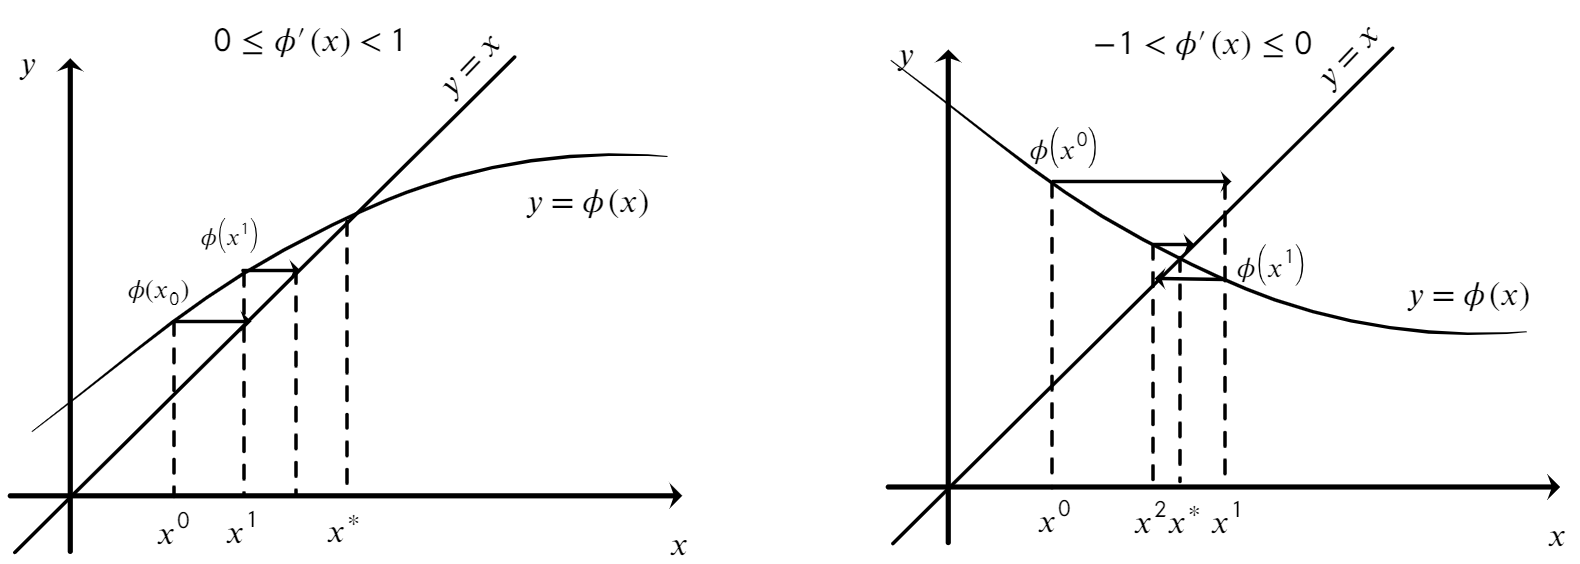
\includegraphics[scale=0.35]{images/img15}
	$$
	В соответствии с формулой
	\begin{equation}
		\varepsilon_{k+1} \approx \varphi'(x^*)\varepsilon_k
	\end{equation}
	сходимость метода осуществляется по закону геометрической прогрессии со знаменателем $q = \varphi'$.
	\\\\
	Итерационная формула
	\begin{equation}
		\label{newton-method-1}
		x^{k+1} = x^k - \dfrac{f(x^k)}{f'(x^k)},\quad k = 0,1,\ldots;\quad x_0
	\end{equation}
	носит название \textbf{метода Ньютона}. Иногда этот метод называют \textbf{методом касательных} (это название следует из геометрического смысла).
	Добавка $x_0$ означает, что начальное приближение задано.
	\\\\
	Исследуем геометрический смысл метода.
	Если рассмотреть уравнение кривой $y = f(x)$, то в точке $x^k$ касательная к ней задается уравнением $$y - f(x^k) = f'(x^k) (x-x^k).$$ Найдем точку пересечения касательной с осью $Ox$: полагая $y=0$, получим $$x= x^k - \dfrac{f(x^k)}{f'(x^k)}.$$ Таким образом строим приближение $x^{k+1}$ и так далее:
	$$
	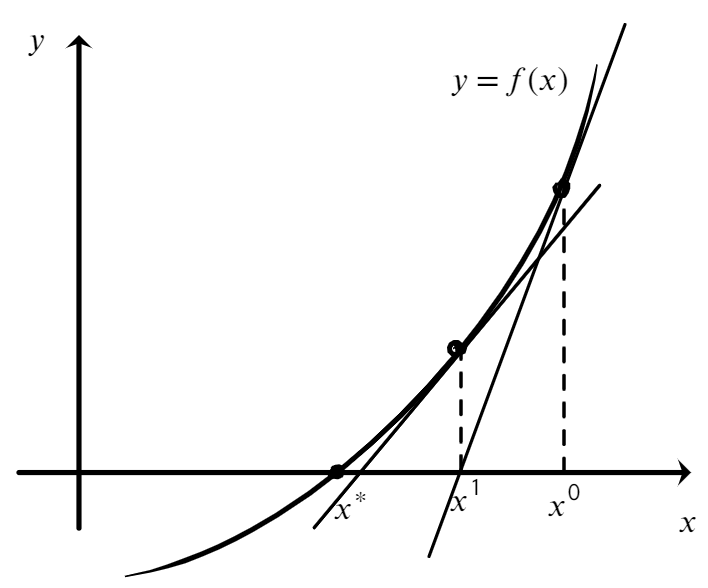
\includegraphics[scale=0.35]{images/img16}
	$$
	То есть мы приближаемся к корню по последовательности касательных прямых.\\\\
	Последовательность $x^k$ построенная по формуле \eqref{newton-method-1} обладает квадратичной сходимостью.

	\begin{table}[h!]
		\centering
		\renewcommand{\arraystretch}{1.5}
		\begin{tabular}{|p{7cm}|p{8cm}|p{2cm}|}
			\hline
			\textbf{Название метода и формула метода} & \textbf{Геометрический смысл метода} & \textbf{Скорость сходимости} \\
			\hline
			
			Метод Ньютона с постоянной производной
			$$x^{k+1} = x^k - \dfrac{f(x^k)}{f'(x^0)},$$ $k=0,1,\ldots$. В этом методе количество операций меньше, чем в классическом. & 
			На каждой итерации используем касательную, построенную в $x^0$ — все последующие касательные параллельны первой.
			$$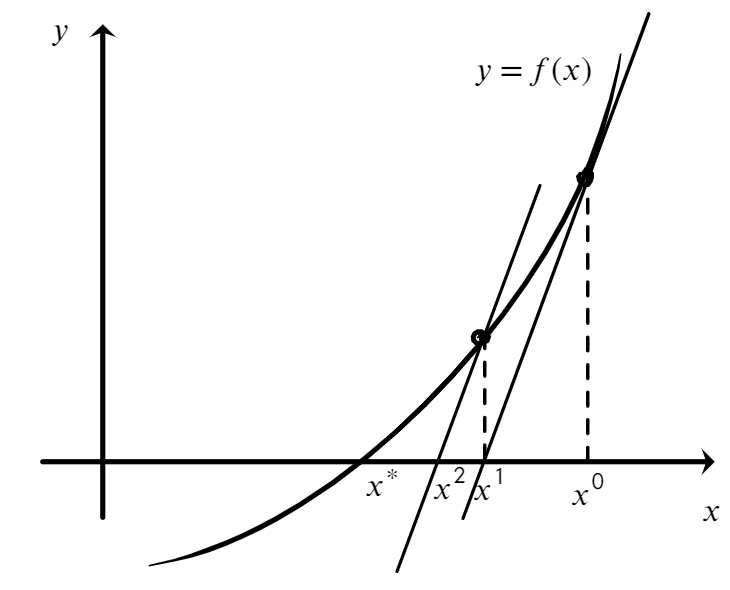
\includegraphics[scale=0.3]{images/img42}$$ & 
			Линейная\\
			\hline
			
			Метод секущих
			$$x^{k+1} = x^k - f(x^k)\dfrac{x^k - x^{k-1}}{f(x^k) - f(x^{k-1})},$$ $k=1,2,\ldots$. Количество операций как и в предыдущем методе. & 
			Проводим секущую через точки $(x^{k-1}, f(x^{k-1}))$ и $(x^k, f(x^k))$. Пересечение секущей с осью Ox даёт новое приближение. 
			$$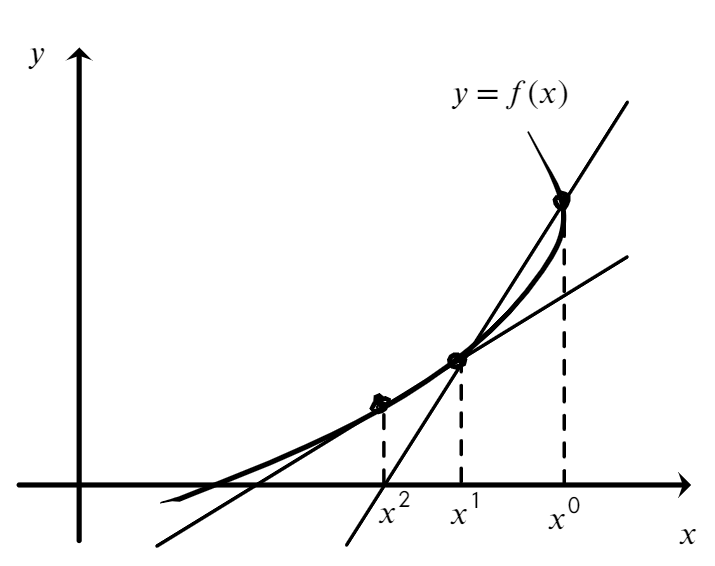
\includegraphics[scale=0.3]{images/img43}$$ & 
			Выше линейной, ниже квадратичной\\
			\hline
			
			Метод хорд
			$$x^{k+1} = x^k - f(x^k)\dfrac{x^k - x^0}{f(x^k) - f(x^0)},$$ $k=1,2,\ldots$. При хорошем начальном приближении метод сходится быстрее остальных. & 
			На каждой итерации строится хорда между $f(x^0)$ и $f(x^k)$. Пересечение хорды с осью Ox даёт новое приближение.  
			$$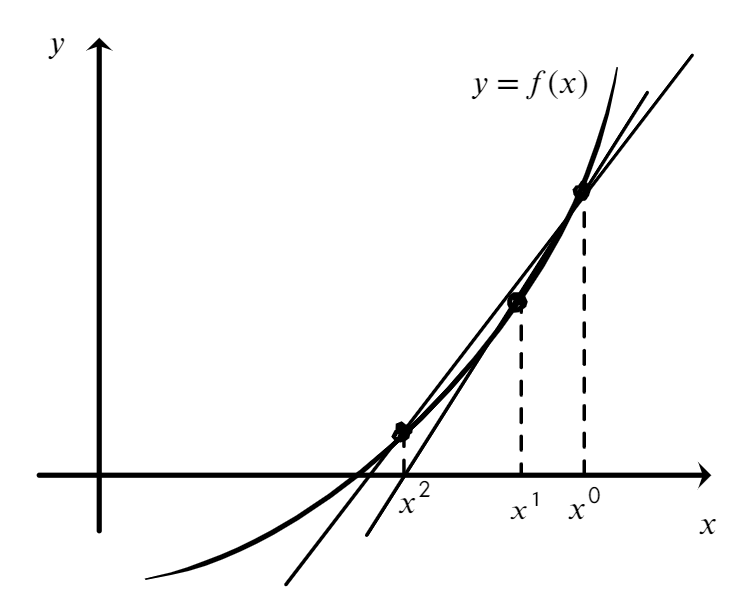
\includegraphics[scale=0.3]{images/img44}$$ & 
			Линейная\\
			\hline
			
		\end{tabular}
		\caption{Сравнительная характеристика модификаций метода Ньютона}
	\end{table}
	
	\begin{table}[h!]
		\centering
		\renewcommand{\arraystretch}{1.5}
		\begin{tabular}{|p{12cm}|p{3cm}|}
			\hline
			\textbf{Название метода и формула метода} & \textbf{Скорость сходимости} \\
			\hline
			
			Метод Стеффенсена
			$$x^{k+1} = \dfrac{x^k \varphi(\varphi(x^k)) - (\varphi(x^k))^2}{\varphi(\varphi(x^k)) - 2 \varphi(x^k) + x^k},\ k=0,1,\ldots; x_0.$$& 
			Квадратичная\\
			\hline
			
			Метод Чебышева
			$$x^{k+1} = x^k - \dfrac{f(x^k)}{f'(x^k)} - \dfrac{f^2(x^k)f''(x^k)}{2(f'(x^k))^3},\ k=1,2,\ldots.$$ &  
			Кубическая\\
			\hline
			
		\end{tabular}
		\caption{Сравнительная характеристика модификаций метода простой итерации}
	\end{table}
	
	Рассмотрим систему нелинейных уравнений (СНУ)
	\begin{equation}
		\begin{cases}
			f_1(x_1,\ldots, x_n) = 0,\\
			\dotfill,\\
			f_n(x_1,\ldots, x_n) = 0.\\
		\end{cases}
	\end{equation}
	или в векторном виде 
	\begin{equation}
		f(x) = 0,\ f=(f_1,\ldots, f_n)^T,\ x = (x_1,\ldots, x_n).
	\end{equation}
	Основные этапы решения:
	\begin{enumerate}
		\item отделение корня;
		\item построение последовательности приближений;
		\item контроль сходимости.
	\end{enumerate}
	Проблема отделения корня для СНУ в общем случае не имеет решений.
	\\\\
	Применение \textbf{метода простой итерации} требует приведения исходной системы к виду удобному для итераций, т.е. канонической форме, и выбора начального приближения $x_0$. Тогда все последующие приближения находятся по формуле 
	\begin{equation}
		\begin{cases}
			x_1^{k+1} = \varphi_1(x_1^k, \ldots, x_n^k),\\
			\dotfill\\
			x_n^{k+1} = \varphi_n(x_1^k, \ldots, x_n^k),
		\end{cases}
		k=0,1,\ldots.
	\end{equation}
	Скорость сходимость по аналогии одномерному случаю линейная, а достаточное условие сходимости 
	\begin{equation}
		\Norm{\dfrac{\partial \varphi(x)}{\partial x}}_1 < 1,\ \Norm{x-x^0}_1\leq \delta.
	\end{equation}
	\begin{table}[h!]
		\centering
		\renewcommand{\arraystretch}{1.5}
		\begin{tabular}{|p{12cm}|p{3cm}|}
			\hline
			\textbf{Название метода и формула метода} & \textbf{Скорость сходимости} \\
			\hline
			
			Метод Зейделя
			\begin{equation}
				\begin{cases}
					x_1^{k+1} = \varphi(x_1^k, x_2^k,\ldots, x_n^k),\\
					x_2^{k+1} = \varphi(x_1^{k+1}, x_2^k,\ldots, x_n^k),\\
					\dotfill\\
					x_n^{k+1} = \varphi(x_1^{k+1}, x_2^{k+1},\ldots, x_n^k),
				\end{cases}\ k=0,1,\ldots
			\end{equation}  & 
			Линейная\\
			\hline
			
			Метод Гаусса-Зейделя
			\begin{equation}
				\begin{cases}
					f_1(x_1^{k+1},x_2^k,\ldots,x_n^k) = 0,\\
					f_2(x_1^{k+1},x_2^{k+1},\ldots,x_n^k) = 0,\\
					\dotfill\\
					f_n(x_1^{k+1},x_2^{k+1},\ldots,x_n^{k+1}) = 0.
				\end{cases}\ k=0,1,\ldots
			\end{equation} 
			Нахождение каждого нового значения $x_i^{k+1}$ требует решения нелинейного уравнения вида $$f_i(x_1^{k+1},\ldots, x_{i-1}^{k+1}, x_i^{k+1}, x_{i+1}^k, \ldots, x_n^k) = 0,$$
			где все $x_j^k, j>i$ известны как значения с предыдущей итерации, а значения $x_j^{k+1}, j<i$ также известны как координаты точек, которые мы ранее вычислили. &  
			-\\
			\hline
			
		\end{tabular}
		\caption{Сравнительная характеристика модификаций метода простой итерации}
	\end{table}
	
	\textbf{Метод Ньютона} для решения СНУ имеет вид
	\begin{equation}
		x^{k+1} = x^k - \Big(\dfrac{\partial f(x^k)}{\partial x}\Big)^{-1}f(x^k),\quad k=0,1,\ldots
	\end{equation}
	Скорость сходимости метода квадратичная, а для существования решения необходимо существование обратной матрицы $\left(\dfrac{\d f}{\d x}\right)^{-1}$.
	\\\\
	Видоизменения метода Ньютона связаны с упрощением вычисления матрицы Якоби $\left(\dfrac{\d f(x^k)}{\d x}\right)$.
	\begin{enumerate}
		\item \textbf{Метод Ньютона с постоянной матрицей Якоби}. 
		Производится замена 
		\begin{equation}
			\left(\dfrac{\d f(x^k)}{\d x}\right)\sim \left(\dfrac{\d f(x^0)}{\d x}\right).
		\end{equation}
		\item \textbf{Дискретный метод Ньютона}.
		Производится замена 
		\begin{equation}
			\left(\dfrac{\d f(x^k)}{\d x}\right)\sim J(x^k, h^k),
		\end{equation}
		где элементы матрицы $J(x^k, h^k)$ вычисляются как 
		$$\dfrac{\d f_i(x_1,\ldots, x_n)}{\d x_j} \approx \dfrac{f_i(x_1,\ldots, x_j,\ldots, x_n) - f_i(x_1,\ldots, x_j-h_j^k,\ldots, x_n)}{h_j^k},$$
		причем $h^k \in \mathbb R^k$, $h_j^k \to 0$.
		\item \textbf{Метод секущих}.
		Производится замена 
		\begin{equation}
			\left(\dfrac{\d f(x^k)}{\d x}\right)\sim J(x^k, h^k),
		\end{equation}
		где элементы матрицы $J(x^k, h^k)$ вычисляются как 
		$$\dfrac{\d f_i(x_1^k,\ldots, x_n^k)}{\d x_j}\approx \dfrac{ f_i(x_1^k,\ldots, x_j^k,\ldots, x_n^k) - f_i(x_1^k,\ldots, x_j^{k-1},\ldots, x_n^k)}{x_j^k - x_j^{k-1}},\ h^k=x^k - x^{k-1}.$$
	\end{enumerate}
	Определим градиентные методы. В этом случае на основе исходной СНУ задается некоторый функционал
	\begin{equation}
		\Phi(x) = \sum_{i=1}^n f_i^2(x_1,\ldots, x_n)
	\end{equation}
	и отыскиваются точки, которые доставляют минимум этого функционала. По \textbf{методу градиентного спуска} итерационная последовательность сходящаяся к решению определяется формулой 
	\begin{equation}
		x^{k+1} = x^k - t_k\operatorname{grad} \Phi(x^k),\ k=0,1,\ldots,\ t\geq 0.
	\end{equation}
	Параметр $t$ выберем из условия минимума функции $\Phi$ в точке $x^{k+1}$:
	\begin{equation}
		t_k = \arg \underset{t}{\min} \Phi(x^k - t\operatorname{grad} \Phi(x^k)).
	\end{equation}
	Рассмотрим задачу нелинейной оптимизации
	\begin{equation}
		f(x) \to \min, \ x\in \mathbb R^n,
	\end{equation}
	где $f(x)\in C^{(2)}$ и в окрестности решения $\dfrac{\d ^2f(x)}{\d x^2}>0$. \textbf{Метод Ньютона для решения задачи нелинейной оптимизации} определяется по итерационной формуле
	\begin{equation}
		x^{k+1} = x^k - \left(\dfrac{\d ^2f(x^k)}{\d x^2} \right)^{-1} \cdot \grad f(x^k),\ k=0,1,\ldots.
	\end{equation}
	
	\section{Приближение функцией. Основные приближения функций и соответствующие алгоритмы}
	\textbf{Проблема приближения функций} формулируется следующим образом \begin{enumerate}
		\item {имея значения функции $f(x_i)$ в одних точках, найти значения функции в других точках;}
		\item {имея некоторую функцию $f(x)$, которую трудно вычислить, заменить ее другой функцией $\varphi(x)$, которую легко вычислить; при этом задача, связанная с приближением функций, состоит в том, чтобы найти такую функцию $\varphi(x)$ и она приближала функцию $f(x)$ с некоторой точностью $\varepsilon$.}
	\end{enumerate}
	Пусть $R$ --- линейное нормированное пространство, $f\in R$ --- элемент, который нужно приблизить. Возьмем в $R$ $(n+1)$ элементов $\varphi_i$, $i=\overline{0,n}$, причем пусть они являются линейно независимыми. С помощью этой системы функций образуем линейное подпространство $\Phi$ всевозможных линейных комбинаций (обобщенных многочленов) вида \begin{equation}
		\varphi = \sum_{i=0}^n c_i\varphi_i,
	\end{equation}
	где $c_i$ --- действительные коэффициенты. Рассмотрим числовое множество 
	\begin{equation}
		\Delta (f,\varphi) = \Norm{f - \varphi},
	\end{equation} где $f$ --- фиксированный элемент, а $\varphi$ --- произвольный элемент из $\Phi$. Это числовое множество ограничено снизу, то есть $\exists \Delta (f)$ такое, что
	\begin{equation}
		\Delta (f) = \underset{\varphi \in \Phi}{\inf} \Delta (f,\varphi).
	\end{equation}
	которое называется \textbf{наилучшим приближением элемента} $f$ на множестве $\Phi$. Элемент $\varphi^*\in \Phi$, называется \textbf{элементом наилучшего приближения} $f$ на $\Phi$.
	\begin{theorem}
		Для любого элемента $f \in R$ в подпространстве $\Phi$ существует элемент наилучшего приближения.
	\end{theorem}
	\noindent
	Нормированное пространство называется \textbf{строго нормированным}, если $$\Norm{f+g} = \Norm{f} + \Norm{g} \Longleftrightarrow f = \lambda g,\ \lambda > 0.$$
	\begin{theorem}
		В строго нормированном пространстве $R$ элемент наилучшего приближения единственный.
	\end{theorem}
	\noindent
	Пусть $R$ --- гильбертово пространство, а $H$ --- его линейное подпространство. Так как гильбертово пространство строго нормировано, то в $H$ существует и единственен элемент наилучшего приближения. 
	\begin{theorem}
		Для того, чтобы элемент $\Phi_0$ был элементом наилучшего приближения $f$ в подпространстве $H$, необходимо и достаточно, чтобы выполнялось соотношение $$f - \Phi_0 \perp H$$
		(то есть $(f - \Phi_0, h) = 0$ $\forall h \in H$).
	\end{theorem}
	\noindent
	Пусть $R = L_2(p)[a,b]$ --- пространство вещественнозначных функций интегрируемых с квадратом на отрезке $[a,b]$ по весу $p(x)$.
	В качестве системы базисных функций возьмем функции $1, x, \ldots, x^n$, или же $\varphi_i = x^i$, $i=\overline{0,n}$. Обобщенный многочлен в этом случае превращается в алгебраический многочлен вида 
	\begin{equation}
		\varphi = P_n(x) = \sum_{i=0}^{n}c_ix^i,\ c_i \in\mathbb R.
	\end{equation}
	Согласно общей теории существует единственный элемент $\varphi^* = P_n^*(x)$, который дает наилучшее приближение данной функции $f$ в пространстве $R$, то есть $$\Delta^2(f) = \Norm{f(x) - P_n^*(x)}^2=\int\limits_a^b p(x)[f(x) - P_n^*(x)]^2dx=\underset{P_n(x)}{\inf}\Norm{f(x) - P_n(x)}^2.$$
	$\bullet$ \textit{Многочлен $P_n^*$ называется \textbf{многочленом наилучшего среднеквадратичного приближения}.}
	\\\\
	Для того, чтобы задать $P_n^*$ нужно решить систему $$(f- P^*_n, x^j) = 0,\ j=0,\ldots, n,$$ то есть
	\begin{equation}
		\begin{cases}
			c_0s_0 + c_1s_1 + \ldots + c_ns_n = m_0,\\
			c_0s_1 + c_1s_2 + \ldots + c_ns_{n+1} = m_1,\\
			\dotfill\\
			c_0s_n + c_1s_{n+1} + \ldots + c_ns_{2n} = m_n.
		\end{cases}
	\end{equation}
	$$s_i = \int\limits_a^b p(x) x^i dx,\ m_j= \int\limits_a^b p(x) f(x) x^j dx,\ i=\overline{0,2n}, j=\overline{0,n}.$$
	$$
		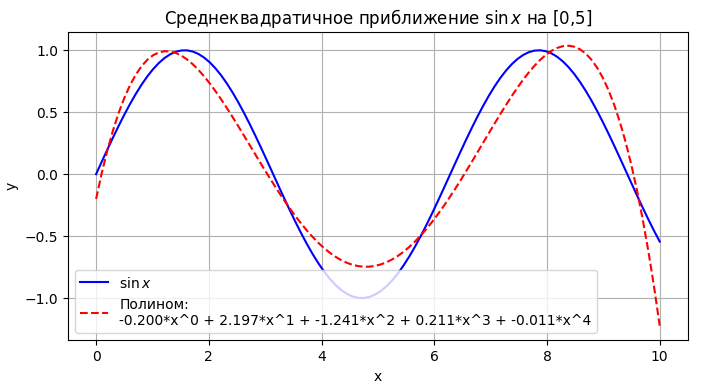
\includegraphics[scale=0.5]{images/img39}
	$$
	\textbf{Интерполированием} называется такой способ приближения функции $f(x)$, $x\in [a,b]$ другой функцией $\varphi(x,a)$, где $a = (a_0,\ldots, a_n)$ --- векторный параметр, когда функция $\varphi(x,a)$ определяется из условия совпадения в точках $x_0,\ldots, x_n$, то есть
		\begin{equation}
			\varphi(x_i,a_0,\ldots, a_n) = f(x_i),\ i =0,1,\ldots, n.
		\end{equation}
		При этом значения $x_i$ называются \textbf{узлами интерполирования}, а совокупность пар чисел $(x_i, f(x_i)), i = \overline{0,n}$ называются \textbf{исходными данными интерполирования}.
	\\\\
	Формула \begin{equation}
		P_n(x) = \sum_{i=0}^{n}l_i(x)f(x_i) = \sum_{i=0}^{n}\dfrac{\omega_{n+1}(x)}{(x-x_i)\omega'_{n+1}(x_i)}f(x_i).
	\end{equation} называется \textbf{формулой Лагранжа для интерполяционного многочлена $P_n$}.\\\\
	Формула \begin{equation}
		r_n(x) = \omega_{n+1}(x) \dfrac{f^{(n+1)}(\xi)}{(n+1)!},\ \xi \in [a,b].
	\end{equation} называется \textbf{представлением остатка интерполирования в форме Лагранжа}.
	\\\\
	Разделенная разность (дискретный аналог производной) для функции определяется по формулам
	$$f(x_i, x_j) = \dfrac{f(x_j) - f(x_i)}{x_j - x_i},\ \ldots,\ f(x_0, \ldots, x_{k+1}) = \dfrac{f(x_1,\ldots, x_{k+1}) - f(x_0,\ldots, x_k)}{x_{k+1} - x_0}.$$
	Формула \begin{multline}
		P_n(x) = f(x_0) + (x-x_0)\cdot f(x_0, x_1) + (x-x_0)(x-x_1)\cdot f(x_0,x_1,x_2) +\ldots \\ \ldots + (x-x_0)\ldots (x-x_{n-1})\cdot f(x_0,\ldots, x_n).
	\end{multline} называется \textbf{формулой Ньютона для интерполяционного многочлена} $P_n(x)$.
	$$
		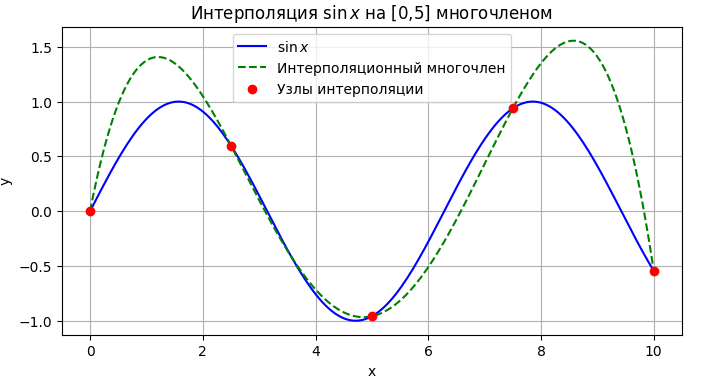
\includegraphics[scale=0.5]{images/img40}
	$$
	Формула \begin{equation}
		r_n(x) = \omega_{n+1}(x)\cdot f(x,x_0,\ldots, x_n).
	\end{equation} --- это \textbf{представление остатка интерполирования в форме Ньютона}.
	\\\\
	\textbf{Сплайн-функцией $m$-ого порядка} называется функция $S_m(x)$, которая удовлетворяет следующим условиям:
	\begin{enumerate}
		\item {На каждом из отрезков $[x_{i-1}, x_i]$, $i=\overline{1,N}$ функция $S_m(x)$ является алгебраическим многочленом степени $m$, то есть} \begin{equation}
			S_m(x) = P_{im}(x) = a_{i0} + a_{i1}x + \ldots + a_{im}x^m,\ x\in [x_{i-1}, x_i],\ i=\overline{1,N}.
		\end{equation}
		\item {Функция $S_m(x)$ непрерывна вместе со своими производными до $(m-1)$-ого порядка включительно во всех внутренних точках, в том числе и в точках $x_i$, $i=\overline{1,N-1}$. То есть} \begin{equation}
			S_m^{(j)}(x_i+0) = S_m^{(j)}(x_i-0),\ j=\overline{0, m-1}, \ i=\overline{1, N-1}.
		\end{equation}
		\item
		\begin{equation}
			S_m(x_i) = f(x_i),\ i=\overline{0,N},
		\end{equation}
	\end{enumerate}
	то функция $S_m(x)$ называется \textbf{интерполяционным сплайном.}\\\\
	Часто рассматривается интерполирование \textbf{кубическим сплайном}, $m=3$.
	Формально он задается 
	\begin{multline}
		S_3(x) = M_{i-1}\dfrac{(x_i - x)^3}{6h_i} + M_{i}\dfrac{(x-x_{i-1})^3}{6h_i} + \left(f_i - M_i\dfrac{h_i^2}{6}\right)\dfrac{x-x_{i-1}}{h_i} +\\+ \left(f_{i-1} - M_{i-1}\dfrac{h_i^2}{6}\right)\dfrac{(x_i - x)}{h_i},\ x\in [x_{i-1}, x_i],\ i = \overline{1,N},
	\end{multline}
	где константы $M_i$ определяются из дополнительных условий
	\begin{equation}
		\dfrac{h_i}{6}M_{i-1} + \dfrac{h_i + h_{i+1}}{3}M_i + \dfrac{h_{i+1}}{6}M_{i+1} = \dfrac{f_{i+1} - f_i}{h_{i+1}} - \dfrac{f_i - f_{i-1}}{h_i},\ i = \overline {1,N-1},
	\end{equation}
	а также граничных условий
	\begin{enumerate}
		\item естественные
		\begin{equation}
			M_0 =0,\ M_N = 0.
		\end{equation}
		\item моменты
		\begin{equation}
			M_0 = f''(a),\ M_N = f''(b).
		\end{equation}
		\item наклоны
		\begin{equation}
			\begin{dcases}
				2M_0 + M_1 = \dfrac{6}{h_1}\left(\dfrac{f_1-f_0}{h_1} - f'(a)\right),\\
				M_{N-1} + 2M_N = \dfrac{6}{h_N}\left(f'(b) - \dfrac{f_N-f_{N-1}}{h_N} \right).
			\end{dcases}
		\end{equation}
	\end{enumerate}
	Таким образом, выбирая к основным условиям граничные условия (16), (17) или (18), можно получить систему линейных уравнений для отыскания коэффициенты $M_i$.
	$$
		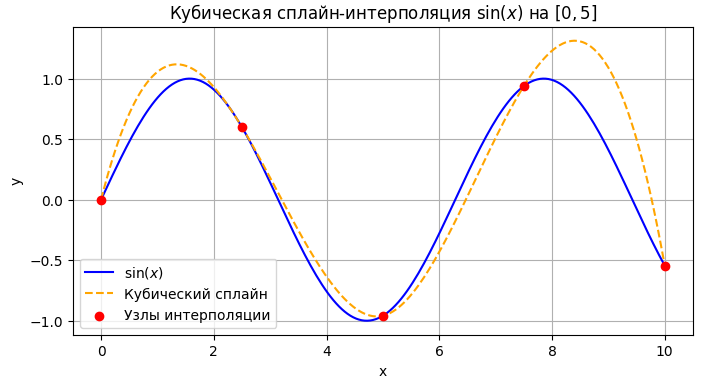
\includegraphics[scale=0.5]{images/img41}
	$$
	\section{Приближенное вычисление интегралов}
	Пусть функция $f(x)$ интегрируемая по Риману на отрезке $[a,b]$. Задача заключается в отыскании значения интеграла $$I = \int\limits_a^b f(x)dx.$$
	Аналитически эту задачу можно решить с помощью формулы Ньютона-Лейбница. Если можно найти для функции $f(x)$ ее первообразную $\mathcal F$, то значение интеграла равно $$I = \mathcal F(b) - \mathcal F(a).$$ Если применение этой формулы невозможно, то используются численные методы.
	Основной подход напрямую связан с заменой подынтегральной функции достаточно близкой, но более простой с точки зрения интегрирования. То есть в качестве \textbf{задачи численного интегрирования} рассматривается задача вычисления значения 
		\begin{equation}
			\label{int-1}
			I(f) = \int\limits_a^b p(x)f(x)dx,
		\end{equation} где $p(x)$ --- это фиксированная ненулевая функция, которая является \textbf{весовой функцией}, а $f(x)$ --- это достаточно гладкая функция, которую будем называть \textbf{интегрируемой функцией.} \\\\
	Следуя теории интерполирования функции, интеграл \eqref{int-1} можно вычислять следующим образом 
	\begin{equation}
		\label{int-2}
		I (f) = \int\limits_a^b p(x) f(x)dx \approx \sum_{k=0}^{n}A_k f(x_k),\ x_k\in[a,b],\ A_k\in \mathbb R.
	\end{equation}
	При этом выражение, стоящее в правой части приближенного равенства \eqref{int-2} называется \textbf{квадратурной суммой}, $A_k$ --- ее коэффициенты, а $x_k$ --- узлы. Само выражение \eqref{int-2} называется \textbf{квадратурной формулой} (или квадратурное правило).\\\\
	Квадратурная формула \eqref{int-2}, коэффициенты $A_k$ которой вычисляются по формуле 
	\begin{equation}
		A_k = \int\limits_a^b p(x) \dfrac{\omega_{n+1}(x)}{(x-x_k)\omega'_{n+1}(x_k)}dx,
	\end{equation}
	называется \textbf{интерполяционной квадратурной формулой}.
	Пусть $f\in C^{n+1}[a,b]$. Тогда выражение для остатка квадратурной формулы
	\begin{equation}
		R_n(f) = \dfrac{1}{(n+1)!} \int\limits_a^b p(x)\omega_{n+1}(x)f^{(n+1)}(\xi)dx.
	\end{equation}
    Пусть $p(x)\equiv1$. Рассмотрим основные интерполяционные квадратурные формулы
    \begin{itemize}
        \item Простейшая квадратурная формула левых прямоугольников и ее остаток
         \begin{equation}
	 	I_{\text{лп}}(f) =(b-a)\cdot f(a),\quad R_\text{лп} (f) = \dfrac{(b-a)^2}{2}f'(\eta), \ \eta \in [a,b].
	 \end{equation}
     Составная квадратурная формула левых прямоугольников и ее остаток
         \begin{equation}
	 	I_\text{лс}(f)= h\sum_{k=0}^{N-1} f(a+kh),\quad R_\text{лс}(f)  = \dfrac{(b-a)^2}{2N}f'(\eta),\ \eta \in [a,b],\quad h = \dfrac{b-a}{N}.
	 \end{equation}
     \item Простейшая квадратурная формула правых прямоугольников и ее остаток
         \begin{equation}
	 	I_{\text{пп}}(f) =(b-a)\cdot f(b),\quad R_\text{пп} (f) = -\dfrac{(b-a)^2}{2}f'(\eta), \ \eta \in [a,b].
	 \end{equation}
     Составная квадратурная формула правых прямоугольников и ее остаток
         \begin{equation}
	 	I_\text{пс}(f)= h\sum_{k=0}^{N-1}f(a+(k+1)h),\quad R_\text{сп}(f)= \dfrac{(b-a)^3}{24}f''(\eta),\ \eta \in [a,b].
	 \end{equation}
     \item Простейшая квадратурная формула средних прямоугольников и ее остаток
         \begin{equation}
	 	I_\text{сп}(f) = (b-a)\cdot f\left(\dfrac{a+b}{2}\right),\quad R_\text{сп}(f) = \dfrac{(b-a)^3}{24}f''(\eta), \ \eta \in [a,b].
	 \end{equation}
     Составная квадратурная формула средних прямоугольников и ее остаток
         \begin{equation}
	 	I_\text{сс}(f) = h\sum_{k=0}^{N-1}f\left(a+\left(k+\dfrac12\right)h\right),\quad R_\text{сс}(f) = \dfrac{(b-a)^3}{24N^2}f''(\eta),\ \eta \in [a,b].
	 \end{equation}
     \item Простейшая квадратурная формула трапеций и ее остаток
         \begin{equation}
	 	I_\text{тп} (f)= \dfrac{b-a}{2}\left(f(a) + f(b)\right),\quad R_\text{тп}(f) = -\dfrac{(b-a)^3}{12}f''(\eta), \ \eta \in [a,b].
	 \end{equation}
     Составная квадратурная формула трапеций и ее остаток
         \begin{equation}
	 	I_\text{тс}(f) = h\left[\dfrac{f(a)+f(b)}{2} + \sum_{k=0}^{N-1}f(kh)\right],\quad R_\text{тс}(f) = -\dfrac{(b-a)^3}{12N^2}f''(\eta),\ \eta \in [a,b].
	 \end{equation}
     \item Простейшая квадратурная формула Симпсона и ее остаток
         \begin{equation}
	 	I_\text{симп п}(f) = \dfrac{b-a}{6}\left(f(a) + 4f\left(\dfrac{a+b}{2}\right) + f(b)\right),\quad R_\text{симп п}(f) = -\dfrac{(b-a)^5}{2880}f^{(4)}(\eta), \ \eta \in [a,b].
	 \end{equation}
     Составная квадратурная формула Симпсона и ее остаток
         \begin{equation}
         \begin{gathered}
             I_\text{симп с}(f) = \dfrac{h}{3}\big(f_0 + f_N + 2(f_2 + f_4 + \ldots + f_{N-2}) + 4(f_1 + f_3 + \ldots + f_{N-1})\big),\ f_i = f(x_i),\\ R_\text{симп с}(f) = -\dfrac{(b-a)^5}{180N^4}f^{(4)}(\eta),\ \eta \in [a,b].
         \end{gathered}
	 \end{equation}
    \end{itemize}
    Применим составную квадратурную формулу при разных параметрах: возьмем два значения $h_1$ и $h_2$ и найдем $I_{h_1}, I_{h_2}$.
    Формула \begin{equation}
	 	R(h,f)\approx \dfrac{I_{h_2}-I_{h_1}}{h_1^m - h_2^m}h_1^m = \dfrac{I_{h_2}-I_{h_1}}{1 - \left(\frac{h_2}{h_1}\right)^m}.
	 \end{equation} дает выражение для главной части остатка квадратурной формулы. Таким образом, мы можем указать алгоритм апостериорной оценки. Мы подбираем шаги $h_1$ и $h_2$ таким образом, чтобы $$|R(h,f)|\leq \varepsilon,$$ тогда интеграл будет считаться вычисленным с заданной точностью. Данное правило называется \textbf{правилом Рунге практической оценки погрешности квадратур}.
	 \\\\
	 Наивысшая степень точности для интерполяционной квадратурной формулы \eqref{int-2} равна $2n+1$. Все их коэффициенты имеют один знак и могут быть вычислены по формуле
	 $$A_k=\dfrac{c_{n+1}}{c_n}\cdot \dfrac{1}{Q_n(x_k)Q_{n+1}'(x_k)},\ k=\overline{0,n},$$
	 $Q_i(x), i=0,1,\ldots,n$ --- это система ортонормированных по весу $p(x)$ многочленов, а $c_n$ и $c_{n+1}$ --- это коэффициенты при старших степенях у многочленов $Q_n(x)$ и $Q_{n+1}(x)$, например,
	 \begin{enumerate}
	 	\item если $p(x) = 1$, $[a,b]=[-1,1]$, то можно выбрать систему многочленов Лежандра;
	 	\item если $p(x) = \dfrac{1}{\sqrt{1-x^2}}$, $[a,b]=[-1,1]$, то можно выбрать систему многочленов Чебышева.
	 \end{enumerate}
	 Пусть в $n$-мерном пространстве $E_n$ необходимо вычислить интеграл по области $\Omega$ вида $$I = \int\limits_\Omega p(x)f(x)dx,$$
	 где $x = (x_1,\ldots, x_n)$, $dx = dx_1\ldots dx_n$, $p(x)$ --- весовая функция, $f(x)$ --- интегрируемая функция. Если случай $n=2$, то рассмотри интеграл по плоской фигуре и в качестве $\Omega$ возьмем прямоугольник $$\Omega = \{(x,y): a\leq x \leq b,\ c \leq y \leq d\}.$$
	 Также возьмем $p(x)\equiv 1$. Тогда интеграл можно записать в виде $$\int\limits_a^b\int\limits_c^d f(x,y)dxdy = \int\limits_a^b F(x)dx,\ F(x) = \int\limits_c^d f(x,y)dy.$$
	 Таким образом, процесс вычисления двойного интеграла сводится к процессу последовательного вычисления одномерных интегралов. Для одномерных интегралов можно применить теорию квадратурных формул.
	 \begin{enumerate}
	 	\item \textbf{Кубатурная формула средних прямоугольников.}
	 	$$I = \int\limits_a^b \int\limits_c^d f(x,y)dxdy\approx S f\left(\dfrac{a+b}{2}, \dfrac{c+d}{2}\right),$$ где $S = (b-a)(c-d)$ -- это площадь прямоугольника $\Omega$.
	 	\item \textbf{Кубатурная формула трапеций.}
	 	$$I=\int\limits_a^b \int\limits_c^d f(x,y)dxdy\approx \dfrac{S}{4}\left[f(a,c) + f(b,c)+f(a,d)+f(b,d)\right].$$
	 	\item \textbf{Кубатурная формула Симпсона.}
	 	\begin{multline*}
	 		I=\int\limits_a^b \int\limits_c^d f(x,y)dxdy\approx \dfrac{S}{36}\left[f(a,c) + f(b,c)+f(a,d)+f(b,d)\right] +\\+ \dfrac S9 \left[f\left(a,\dfrac{c+d}{2}\right) + f\left(\dfrac{a+b}{2},c\right)+f\left(\dfrac{a+b}{2},d\right)+f\left(b,\dfrac{c+d}{2}\right) +4f\left(\dfrac{a+b}{2},\dfrac{c+d}{2}\right)\right].
	 	\end{multline*}
	 \end{enumerate}
	\section{Методы численного решения начальных и граничных задач для обыкновенных дифференциальных уравнений}
	Не ограничивая общности, рассмотрим задачу Коши для одного обыкновенного дифференциального уравнения первого порядка вида 
	\begin{equation}
		\label{cauchi-1}
		\begin{cases}
			u'(x) = f(x, u(x)),\ x_0 \leq x \leq X,\\
			u(x_0) = u_0,
		\end{cases}
	\end{equation} где $x$ --- это независимая переменная, $f(x, u(x))$ --- заданная функция.
	Если правая часть уравнения непрерывна и удовлетворяет условию Липшица по переменной $u$, то решение задачи Коши \eqref{cauchi-1} единственно и непрерывно зависит от координат начальной точки. Таким образом, задача \eqref{cauchi-1} является корректно поставленной.
	\\\\
	Идея одношаговых методов заключается в следующем. Рассмотрим исходную задачу \eqref{cauchi-1} и по формуле из теоремы Пикара-Линделефа проинтегрируем уравнение, но не на промежутке $[x_0,x]$, а на $[x_j, x_{j+1}]$. Тогда \begin{equation}
		\label{approx-formula}
		u(x_{j+1}) = u(x_j) + \int\limits_{x_j}^{x_{j+1}}f(t, u(t))dt.
	\end{equation}
	Уравнение \eqref{approx-formula} связывает значение решения исходного уравнения в точках $x_{j+1}$ и $x_j$. Указав способ вычисления интегралов в правой части, мы можем получить соответствующее вычислительное правило.
	\\\\
	Для построения одношаговых правил любого наперед заданного порядка точности существует способ, основанный на введении трех наборов параметров:
	\begin{equation}
		\label{params}
		\begin{cases}
		\alpha_1,\ldots, \alpha_q \quad (\alpha),\\
		\begin{gathered} 
			\beta_{10} \hfill \\ 
			\beta_{20},\ \beta_{21}\hfill  \\
			\dots\dots\dots \hfill \\
			\beta_{q0}, \beta_{q1},\ldots, \beta_{qq-1} \hfill \\
		\end{gathered}\quad (\beta)\\
		A_0,\ldots, A_q \quad (A)
	\end{cases}
	\end{equation}
	Используя эти параметры, мы можем записать метод 
	\begin{equation}
		\label{ode-method}
		y_{j+1} = y_j + \sum_{i=0}^q A_i\varphi_i,
	\end{equation}
	\begin{equation}
		\label{conditions}
		\begin{cases}
		\varphi_0 = hf(x_j, y_j),\\
		\varphi_1 = hf(x_j + \alpha_1 h_, y_j + \beta_{10}\varphi_0),\\
		\varphi_2 = hf(x_j + \alpha_2h, y_j + \beta_{20}\varphi_0 + \beta_{21}\varphi_1),\\
		\dotfill\\
		\varphi_q = hf(x_j + \alpha_q h, y_j + \beta_{q0} \varphi_0 + \ldots + \beta_{qq-1}\varphi_{q-1}).
	\end{cases}
	\end{equation}
	Семейство методов \eqref{ode-method}-\eqref{conditions} при известных значениях параметров \eqref{params} называются \textbf{методами Рунге-Кутта.}\\\\
	Весь смысл введения параметров заключается в том, чтобы за счет их выбора обеспечить требуемое свойство данного метода, а именно точность. Выбор параметров $\alpha, \beta, A$ осуществляется на основании требования, чтобы погрешность формулы \eqref{ode-method} была величиной порядка $r_j = O(h^{k+1})$, где $k$ --- требуемый порядок метода. Таким образом, мы можем построить метод любого порядка.
	\\\\
	Рассмотрим две методики, которые приняты в литературе, для определения параметров $\alpha, \beta, A$.
	\begin{enumerate}
		\item Предполагаем, что правая часть исходного уравнения \eqref{cauchi-1} является достаточно гладкой функцией. Рассмотрим невязку формулы \eqref{ode-method} над точным решением в точке $x_j$. Мы можем записать разложение этой функции в ряд Тейлора в окрестности точки $0$:
		$$r_j(h) = \sum_{l=0}^{k}\dfrac{h^l}{l!} r^{(l)}_j(0) + \dfrac{h^{k+1}}{(k+1)!}r_j^{(k+1)}(\theta h),\ 0 < \theta < 1.$$
		Основным требованием для обеспечения требуемого порядка есть условие, чтобы \begin{equation}
			\label{coef-conditions}
			r_j^{(l)}(0) = 0,\ l = 0,1\ldots, k
		\end{equation}
		Условие \eqref{coef-conditions} и есть условие для выбора коэффициентов. При этом, учитывая разложение, мы можем утверждать, что $$r_j(h)= \dfrac{h^{k+1}}{(k+1)!}r^{k+1}(\theta h)$$
		Таким образом, методы Рунге-Кутта $k$-ого порядка точности могут быть построены за счет выполнения условия \eqref{coef-conditions}, которое в свою очередь может быть выполнено за счет выбора параметров \eqref{params}.
		\item Основан на требовании, чтобы разложения функций $u(x_j + h) - u(x_j)$ и
		$\sum_{i=0}^{q}A_i \varphi_i$, где $\varphi_i$ вычислены над точным решением, по степеням $h$ совпадали до членов с возможно более высокими степенями $h$. Это возможно сделать за счет выбора параметров $\alpha, \beta, A$. Таким образом, мы добьемся требуемого порядка точности метода.
	\end{enumerate}
	Способ построения многошаговых методов, как и в случае одношаговых, базируется на интегральном соотношении, которое можно записать в следующем виде 
	\begin{equation}
		\label{int-formula}
		u(x_{j+1}) = u(x_j)  + \int\limits_{x_j}^{x_{j+1}} u'(t)dt.
	\end{equation}
	Предполагая, что в точках $x_j, x_{j-1},\ldots, x_{j-k}$ мы знаем приближенные значения нашего решения, заменим подынтегральную функцию $u'(t)$ ее интерполяционным приближением по этим значениям:
	$$u'(t) \approx \varphi(t, y_{j-k}, \ldots, y_j).$$
	Очевидно, что после такой замены интеграл в формуле \eqref{int-formula} может быть вычислен с учетом погрешности интерполирования. В результате получим некоторый \textbf{явный $(k+1)$-шаговый метод решения задачи Коши}.\\\\
	Можно интерполировать подынтегральную функцию по узлам $x_{j+1}, x_j,\ldots, x_{j-k}$. А значит привлекается значение $y_{j+1}$, которое в данной формуле является неизвестной. Тогда мы получим некоторый \textbf{неявный $(k+2)$-шаговый метод решения задачи Коши.} \\\\
	Многошаговые методы, использующие в качестве интерполирующей функции алгебраические многочлены получили название \textbf{методов Адамса.}\\\\
	Итак, в случае равномерного шага мы получим формулу следующего вида \begin{equation}
		\label{adams-1}
		y_{j+1} = y_j + h\sum_{i=0}^{k}A_i f(x_{j-i}, y_{j-i}),
	\end{equation}
	где коэффициенты вычисляются через интегралы $$A_i = \dfrac{(-1)^i}{i! (k-i)!}\int\limits_0^1 \dfrac{\alpha(\alpha+1)\ldots (\alpha+k)}{\alpha+i}d\alpha.$$
	Метод \eqref{adams-1} называется \textbf{явным экстраполяционным методом Адамса.}\\\\
	Можно показать, что $(k+1)$-шаговый экстраполяционный метод Адамса является методом $(k+1)$-ого порядка точности.
	Особенностью реализации является необходимость задавать первые $k$ значений приближенного решения $y_j$, $j=\overline{1,k}$.\\\\
	На практике, как правило, для определения начала таблицы используются одношаговые методы. Причем с единственным ограничением: чтобы эти значения были получены с погрешностью, соответствующей погрешности метода. \\\\
	В случае интерполяционных методов мы получим формулу
	\begin{equation}
		\label{adams-2}
		y_{j+1} = y_j + h\sum_{i=-1}^{k}A_i f(x_{j-i}, y_{j-i}),
	\end{equation}
	где коэффициенты вычисляются как 
	$$A_i = \dfrac{(-1)^{i+1}}{(i+1)! (k-i)!}\int\limits_0^1\dfrac{(\alpha-1)\alpha(\alpha+1)\ldots(\alpha+k)}{\alpha+i}d\alpha$$
	Метод \eqref{adams-2} называется \textbf{интерполяционным методом Адамса.} Этот метод $(k+2)$-ого порядка точности.\\\\
	Методы Адамса по сравнению с одношаговыми методами являются более экономичными.\\\\
	Формула 
	\begin{equation}
		R(t_j)\approx\dfrac{y_{\tau_1}-y_{\tau_2}}{\tau_2^k - \tau_1^k}
	\end{equation}
	дает возможность после проведения вычислений до точки $t_j + \tau$ с шагами $\tau_1$ и $\tau_2$ получить приближенные значения величин погрешностей для каждого из приближенных значений решения $y_{\tau_1}$, $y_{\tau_2}$. Это правило называется \textbf{правилом Рунге}. Кроме того при заданной границе $\epsilon$ допустимой погрешности на основании приближенного равенства \begin{equation}
		\epsilon \approx |R(t_j)|\tau_\epsilon^k
	\end{equation}
	по результатам вычислений можно выбрать практически более  приемлемое при данных требованиях к точности значение шага 
	\begin{equation}
		\tau_\epsilon = \sqrt[k]{\epsilon \left|\dfrac{\tau_2^k - \tau_1^k}{y_{\tau_1}-y_{\tau_2}}\right|}.
	\end{equation}
	\textbf{Метод редукции} предназначен для решения линейных краевых задач и основан на сведении линейной краевой задачи к решению задачи Коши.\\\\
	Определим дифференциальную задачу с граничными условиями с помощью линейных дифференциальных операторов $L$, $l$
	\begin{equation}
		\label{gr-ode}
		\begin{dcases}
			Lu \equiv u^{(n)}(x) + p_1(x) u^{(n-1)}(x) + \ldots + p_{n-1}(x)u'(x) + p_n(x)u(x) = f(x),\ a < x < b,\\
			l_j(x) = \sum\limits_{i=0}^{n-1}\left[\alpha_{ij} u^{(i)} (a) + \beta _{ij}u^{(i)}(b)\right] = \mu _j,\ j = \overline{1,n},
		\end{dcases}
	\end{equation}
	где заданы $\alpha_{ij}, \beta_{ij} = \operatorname{const}$, а количество условий должно совпадать с порядком уравнения.
	Из теории дифференциальных уравнений известно, что общее решение задачи \eqref{gr-ode} представимо в виде линейной комбинации $$u(x) = u_0(x) + \sum_{i=1}^{n}C_iu_i(x),$$
	где $u_0(x)$ --- это некоторое частное решение неоднородного уравнения, а $u_i(x)$ --- решения соответствующего однородного уравнения, причем $u_i(x)$ образуют линейную независимую систему. В формуле (5) $C_i$ --- это произвольные постоянные, конкретные значения которых определяются граничным.
	Функцию $u_0(x)$ будем определять из следующей задачи Коши
	$$\begin{cases}
		L u_0(x) = f(x),\ a<x< b,\\
		u_0(a) = 0,\\
		\dotfill\\
		u_0^{(n-1)}(a) = 0.
	\end{cases}$$
	Функции $u_i(x)$ будем находить из следующей задачи Коши
	$$
	\begin{cases}
		L u_i(x) = 0,\\
		u_i^{(j)}(a)  = \delta_i^{j+1},\ j = \overline{0,n-1}
	\end{cases}
	$$
	Такой выбор начальных условий обеспечивает линейную независимость функций $u_i(x)$.
	Таким образом, решение краевой задачи \eqref{gr-ode} свелось к решению $(n+1)$ задач Коши.
	\\\\
	Будем рассматривать подход, когда дифференциальная задача, которая представима в виде операторного уравнения $$Au = f$$ сводится к построению приближения $u_n(x)$ к искомой функции $u(x)$ как линейную комбинацию
	$$u_n(x) = \varphi_0 + \sum_{i=1}^n a_i \varphi_i(x),$$
	где $\varphi_i(x)$ -- базисные функции, а $a_i$ -- это коэффициенты подлежащие определению. Если коэффициенты $a_i$ определяются из условия минимума функционала соответствующего рассматриваемой вариационной задаче $$(Au,u)-2(f,u)\to \underset{u}{\min},$$ то мы получим, так называемые, \textbf{вариационные методы}, среди которых \textbf{метод Ритца}, \textbf{метод наименьших квадратов}. Если определять $a_i$ из условия ортогональности невязки к каждой из базисных функций $$(Au_n - f, \varphi_i) =0,$$ то мы придем к, так называемому, \textbf{проекционному методу}, среди которых \textbf{метод Галеркина}, \textbf{метод моментов}.\\\\
	Оба эти варианта приводят к системам линейных алгебраических уравнений.
	\\\\
	Дифференциальную задачу, представленную операторным уравнением, мы можем также решать \textbf{сеточными методами}. Их суть заключается в замене дифференциальных операторов $A$ разностными операторами $A_h$, определенными на некоторой \textbf{сетке узлов} по некоторому \textbf{шаблону}. Исходное же непрерывное решение $u(x)$ заменятся дискретной сеточной функцией $y(x)$, являющейся \textbf{сеточной аппроксимацией} исходного непрерывного решения $u(x)$. В итоге решение исходной задачи заменяется решением \textbf{разностных уравнений}, которые в свою очередь являются системой линейных алгебраических уравнений.
	\chapter{Математические методы принятия решений}

    \section{Симплекс-метод как основной метод решения задач линейного программирования}
    \textbf{Задача линейного программирования} (ЛП) --- это задача максимизации (минимизации) линейной функции на множестве, заданном системой линейных уравнений и неравенств. По форме записи выделяют \textbf{каноническую задачу ЛП}
    \begin{equation}
    \label{lp}
    \begin{cases}
        c^\top x \to \max, \\ Ax = b, \\ d_{-} \leq x \leq d^{+}.
    \end{cases}
    \end{equation}
    В ЛП, исходя из физического смысла элементов, называют: $c = (c_J)$~--- \textbf{вектором стоимости} (координаты $c_j$~--- \textbf{коэффициентами стоимости}), вектор $b = (b_I)$~--- \textbf{вектором основных ограничений (вектором ресурсов)}, матрицу $A = (a_{ij})$~--- \textbf{матрицей условий} (\textbf{матрицей ресурсов}), столбцы~--- $a_j = (a_{ij})_{i \in I}$, $j \in J$, матрицы $A$~--- \textbf{векторами условий}. Здесь $I = \{1, 2, \ldots, m\}$, $J = \{1, 2, \ldots, n\}$.
\\\\
Предположим, что ограничения задачи \eqref{lp} совместны. Каждый вектор $x \in \mathbb{R}^n$, удовлетворяющий ограничениям задачи, называется \textbf{планом}. Тогда
\[
    X = \{x \in \mathbb{R}^n : Ax = b, \, d_{-} \leq x \leq d^{+}\}
\]
называется \textbf{множеством планов}.
\\\\
План $x^0$, являющийся решением задачи, т.е. $c^\top x^0 = \max c^\top x$, $x \in X$, называют \textbf{оптимальным планом}.
\\\\
В ЛП наряду с канонической формой широко используется \textbf{нормальная задача ЛП}
\begin{equation}
\label{lp-2}
\begin{cases}
    c^\top x \to \max, \\ Ax \leq b, \\ d_{-} \leq x \leq d^{+},
\end{cases}
\end{equation}
которая, как и задача \eqref{lp}, является общей, т.е. к ней можно свести любую задачу ЛП.
\\\\
При $n=2$ задачу ЛП удобно решать \textbf{графическим методом}. Его суть состоит в следующем. Система линейных неравенств на плоскости задает выпуклый многоугольник (возможно неограниченный). Это и есть множество планов. Известно, что любая функция $f(x)$ возрастает в направлении градиента $\nabla f(x) = (\partial f/\partial x_1, \ldots, \partial f/\partial x_n)$. Для линейной функции задачи ЛП градиентом является вектор $c$. Значит, максимум функции $c^\top x$ достигается в направлении вектора $c$. Поэтому, двигаясь от произвольной точки $c$ до тех пор, пока множество уровней не только касается множества $X$, найдем точку $x^0$, в которой минимум уровня в последний раз касается множества $X$, и будет точка максимума. Заметим, что множество уровней в последний раз может касаться множества планов не в одной точке~--- это ребро. В этом случае каждая точка этого ребра~--- оптимальный план. Возможна и такая ситуация, когда множество планов не ограничено, и все точки с направления в сторону неограниченности множества планов, так что точки уровня, равные множества уровней с множеством планов можно удалить в бесконечность. В таком случае целевая функция неограниченно возрастает на множестве планов, и задача не имеет решения.
$$
    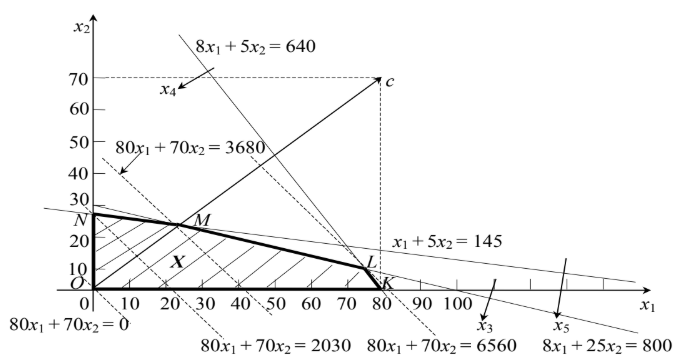
\includegraphics[width=0.5\linewidth]{images/img36.png}
$$
Рассмотрим задачу в канонической форме \eqref{lp}. Пусть выполняются условия: 
\begin{enumerate}
    \item $X \neq \varnothing$;
    \item $\operatorname{rank} A = m$ ($m < n$).
\end{enumerate}
\textbf{План} $x$ называется \textbf{базисным}, если $n-m$ его координат принимают одно из граничных значений ($x_j = d_j,\, d_j^*$), а остальным $m$ координатам
\begin{equation}
\label{coords}
    x_{j_1}, \ldots, x_{j_m}
\end{equation}
соответствуют линейно независимые векторы условий
\begin{equation}
\label{vecs}
    a_{j_1},\ldots,a_{j_m}.
\end{equation}
Множество $J_B = \{j_1, \ldots, j_m\}$ назовём \textbf{базисным множеством индексов}, $J_H = \{1, \ldots, n\} \setminus J_B$ --- \textbf{небазисным}, векторы \eqref{vecs} --- \textbf{базисом базисного плана}, координаты $x_j$ --- \textbf{базисными координатами} плана, остальные --- \textbf{небазисными}, матрицу $A_B = (a_j,\, j\in J_B)$ --- \textbf{базисной матрицей}.
\\\\
\textbf{Базисный план} $x$ называется \textbf{невырожденным}, если базисные координаты не лежат на границах: $d_j < x_j < d_j^*$, $j \in J_B$.
\\\\
\textbf{Задача ЛП} называется \textbf{невырожденной}, если все её базисные планы не вырождены.
\\\\
По базисной матрице $A_B$ подсчитаем m-вектор
\begin{equation}
\label{potencia}
    u' = c'_B A_B^{-1}
\end{equation}
(он называется \textbf{вектором потенциалов}), а также числа (\textbf{оценки})
\begin{equation}
\label{estimates}
    \Delta_j = c_j - u' a_j = c_j - c'_B A_B^{-1} a_j, \quad j = 1, \ldots, n.
\end{equation}
\begin{theorem}
    [критерий оптимальности базисного плана] Для оптимальности базисного плана $x$ с базисной матрицей $A_B$ достаточно, а в случае его невырожденности и необходимо, чтобы выполнялись соотношения:
\begin{equation}
    \Delta_j \leq 0 \text{ при } x_j = d_j, \quad \Delta_j \geq 0 \text{ при } x_j = d_j^*, \quad j \in J_H.
\end{equation}
\end{theorem}
\noindent
\textbf{Задача двойственная задача к канонической задаче} \eqref{lp} имеет вид
\begin{equation}
\label{dvost}
    \begin{cases}
        \psi(\lambda) = b' y + w' d_{-} - v' d^{+} \to \min,\\
        A'_y + w - v = c,\\
        w \geq 0,\ v \geq 0,
    \end{cases}
\end{equation}
где $\lambda = (y,w,v)$. Ограничения $A'_y + w - v = c$ называются \textbf{основными ограничениями}, ограничения $w \geq 0,\ v \geq 0$ --- \textbf{прямыми ограничениями} двойственной задачи \eqref{dvost}.
\begin{theorem}
    [двойственности]
    Для существования решения $x^0$ прямой задачи \eqref{lp} необходимо и достаточно существование решения $\lambda^0$ двойственной задачи, при этом выполнится равенство $\varphi(x^0) = \psi(\lambda^0)$.
\end{theorem}
\noindent
\textbf{Задача двойственная задача к нормальной задаче} \eqref{lp-2} имеет вид
\begin{equation}
\begin{cases}
     b' y \to \min,\\
    A'_y \geq c, \\ x \geq 0.   
\end{cases}
\end{equation}
\noindent
\textbf{Физический смысл двойственных переменных}: $y_i^0 = u_i^0$~--- \textbf{мера (степень) чувствительности} максимальной прибыли к изменению $i$-го ресурса: если $y_i^0 > 0$, то увеличение объёма $i$-го ресурса ведёт к увеличению максимальной прибыли и тем эффективнее, чем больше $y_i^0$; при $y_i^0 < 0$ увеличение максимальной прибыли ведёт к уменьшению объёма $i$-го ресурса. $w_j^0$~--- мера (степень) чувствительности максимального значения целевой функции к изменению значения $j$-й верхней границы, а $-v_j^0$~--- к изменению значения $j$-й нижней границы.
	\section{Метод множителей Лагранжа в нелинейном и выпуклом программировании}
	\textbf{Задача нелинейного программирования со смешанными ограничениями} формулируется следующим образом
	\begin{equation}
		\label{nlp}
		\begin{cases}
			f(x)\to \min,\ x \in \mathbb R^n,\\
			g(x)\leq 0,\\
			h(x) = 0,
		\end{cases}
	\end{equation}
	где $f(x)$ -- скалярная функция, определенная на множестве $\mathbb R^n$, $g(x)$ -- $m$-мерная вектор-функция, а $h(x)$ -- $k$-мерная вектор-функция, $k<n$. Элементы $x\in \mathbb R^n$ называются \textbf{планами задачи}, а функция $f(x)$ -- \textbf{целевой функцией}. В частном случае одно или оба дополнительным условия могут отсутствовать, тогда задача называется \textbf{задачей на безусловный экстремум}.
	\\\\
	Если план $x^0$ удовлетворяет условию $f(x^0) = \min f(x)$, $x \in \mathbb R^n$, то он называется \textbf{глобально оптимальным планом}. Если на плане $x^0$ для некоторого $\epsilon > 0$ выполняется равенство $f(x^0) = \min f(x)$, $\Norm{x - x^0}<\epsilon$, $x \in \mathbb R^n$, то план $x^0$ называется \textbf{локальном оптимальным планом} задачи \eqref{nlp}.
	\\\\
	План \(x^* \in X\) называется \textbf{регулярным}, если векторы-градиенты 
	\[
	\frac{\partial g_i(x^*)}{\partial x}, \, i \in I_a(x^*), \quad \frac{\partial h_j(x^*)}{\partial x}, \, j = 1, \dots, k,
	\]
	линейно независимы.
	\\\\
	\textbf{Условиями регулярности множества планов} являются любое из следующих:
	\begin{enumerate}
		\item Выпуклость функций \(g_i(x), \, i = 1, \dots, m\), отсутствие ограничений-равенств и существование точки \(x^* \in X\) такой, что \(g(x^*) < 0\) (условие Слейтера);
		\item Линейность функций \(g(x), \, h(x)\);
		\item Векторы-градиенты \(\frac{\partial g_i(x^0)}{\partial x}, \, i \in I_a(x^0), \, \frac{\partial h_j(x^0)}{\partial x}, \, j = 1, \dots, k,\) линейно независимы.
	\end{enumerate}
	При исследовании задач на условный минимум используется \textbf{классическая функция Лагранжа}
	\begin{equation}
		\label{classic-lagrange}
		F(x, \lambda, \mu) = f(x) + \lambda^T g(x) + \mu^T h(x).
	\end{equation}
	Это возможно лишь при выполнении одного из трех условий регулярности.
	\\\\
	Числа \(\lambda_i, \, i = 1, \dots, m,\) \(\mu_j, \, j = 1, \dots, k,\) называют \textbf{множителями Лагранжа}, а вектор \((\lambda, \mu), \, \lambda = (\lambda_1, \dots, \lambda_m), \, \mu = (\mu_1, \dots, \mu_k),\) — \textbf{вектором Лагранжа}.
	\begin{theorem}
	[классическое правило множителей Лагранжа] Пусть \(x^0\) — регулярный локально оптимальный план задачи \eqref{nlp}. Тогда существует единственный вектор Лагранжа \((\lambda^0, \mu^0)\), такой, что выполняются соотношения:
	\begin{enumerate}
		\item \textbf{условие неотрицательности:} \(\lambda^0 \geq 0\),
		\[
		\]
		\item \textbf{условие дополняющей нежёсткости:} \(\lambda^0 g(x^0) = 0\),
		\[
		\]
		\item \textbf{условие стационарности:}
		\[
		\frac{\partial F(x^0, \lambda^0, \mu^0)}{\partial x} = 0.
		\]
	\end{enumerate}
	\end{theorem}
	\noindent
	План \(x^* \in \mathbb R^n,\) для которого справедливы условия теоремы, называется \textbf{условно стационарным}.
	Таким образом, локально оптимальные планы задачи \eqref{nlp} находятся среди условно стационарных планов.
	\\\\
	Множество $X \subset \mathbb R^n$ называется \textbf{выпуклым}, если $x(\lambda) = \lambda x^1 + (1-\lambda)x^2 \in X$ при всех $x^1,x^2 \in X$, $\lambda \in [0,1]$, то есть если вместе с любыми своими двумя точками множество $X$ содержит соединяющий их отрезок
	$$
		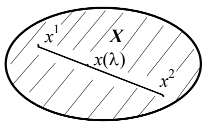
\includegraphics[scale=0.6]{images/img27}
	$$
	Функция $f(x)$ определенная и конечная на выпуклом множестве $X \subset \mathbb R^n$ называется \textbf{выпуклой}, если для любых $x^1, x^2 \in X$ выполняется неравенство
	\begin{equation}
		f(\lambda x^1 + (1-\lambda)x^2)\leq \lambda f(x^1) + (1-\lambda)f(x^2),\ \forall \lambda \in [0,1].
	\end{equation}
	\textbf{Основная задача выпуклого программирования} имеет вид
	\begin{equation}
		\label{vp}
		\begin{cases}
			f(x)\to \min,\ x \in Q,\\
			g(x) \leq 0,
		\end{cases}
	\end{equation}
	где $f(x)$, $g_i(x)$, $i=1,\ldots,m$ ($g(x) = (g_1(x),\ldots, g_m(x))$) -- выпуклые (вогнутые) функции, $Q \subset \mathbb R^n$ -- выпуклое множество.
	\\\\
	Вектор $x$, удовлетворяющий всем ограничениям задачи \eqref{vp}, называется \textit{планом}, множество 
	$
	X = \{ x : g(x) \leq 0,\, x \in Q \}
	$
	-- \textit{множеством планов} задачи \eqref{vp}. В силу свойств выпуклых множеств и выпуклых функций, $X \subset \mathbb{R}^n$ -- выпуклое множество.
	\\\\
	План $x^0$, для которого 
	$
	f(x^0) = \min f(x),\, x \in X,
	$
	называется \textit{оптимальным планом} задачи \eqref{vp}. Если целевая функция $f(x)$, $x \in X$, -- строго выпуклая функция, то оптимальный план единственный.
	\\\\
	Говорят, что множество планов $X$ задачи \eqref{vp} \textbf{регулярно} (удовлетворяет \textbf{условию Слейтера}), если на некотором плане $x^*$ выполняется неравенство $g(x^*) < 0$.
	\\\\
	Решение задачи выпуклого программирования сводится к нахождению седловых точек функции Лагранжа
	\[
	F(x, \lambda) = f(x) + \lambda' g(x),\, x \in Q,\, \lambda \geq 0,\, \lambda \in \mathbb{R}^m
	\]
	($\lambda = (\lambda_1, \ldots, \lambda_m)$ -- вектор множителей Лагранжа).
	\\\\
	Пара $\{ x^*, \lambda^* \}$, $x^* \in Q$, $\lambda^* \geq 0$, -- \textbf{седловая точка функции Лагранжа}, если для любых $x \in Q$, $\lambda \geq 0$ выполняются неравенства
	\[
	F(x^*, \lambda) \leq F(x^*, \lambda^*) \leq F(x, \lambda^*).
	\]
	Теоремы о существовании седловых точек функции Лагранжа называют \textbf{теоремами Куна--Таккера}, по имени ученых, получивших первые результаты для гладких задач.
	\\\\
	Для гладкой задачи выпуклого программирования с регулярным множеством планов (с гладкими выпуклыми функциями $f(x)$, $g(x)$ и множеством $Q = \{ x \in \mathbb{R}^n : x \geq 0 \}$) справедлива
	\begin{theorem}
		[Куна-Таккера]
		Для оптимального плана $x^0$ в гладкой задаче \eqref{vp} с регулярным множеством планов необходимо и достаточно существования такого $m$-векторна $\lambda^0\geq 0$, что выполняются условия Куна--Таккера:
		\[
		\begin{aligned}
			&\frac{\partial F(x^0, \lambda^0)}{\partial x} \geq 0, \\
			&\frac{\partial F'(x^0, \lambda^0)}{\partial x}x^0 = 0, \quad x^0 \geq 0, \\
			&\frac{\partial F(x^0, \lambda^0)}{\partial \lambda} \leq 0, \\
			&\frac{\partial F'(x^0, \lambda^0)}{\partial \lambda}\lambda^0 = 0, \quad \lambda^0 \geq 0,
		\end{aligned}
		\]
		или, что то же самое, пара $\{x^0, \lambda^0\}$ является седловой точкой функции Лагранжа $F(x, \lambda)$ и выполняется условие дополняющей нежесткости $g'(x^0)\lambda^0 = 0$.
	\end{theorem}
	\noindent
	В общем случае справедливо следующее утверждение.
	\begin{theorem}
		Для существования оптимального плана $x^0$ задачи выпуклого программирования \eqref{vp} с регулярным множеством планов необходимо и достаточно существование $m$-вектора $\lambda^0 \geq 0$ такого, что пара $\{x^0, \lambda^0\}$ является седловой точкой функции Лагранжа. При этом выполняется условие дополняющей нежесткости $g'(x^0)\lambda^0 = 0$.
	\end{theorem}
	\section{Метод ветвей и границ, динамическое программирование для решения конечномерных экстремальных задач}
	Рассматривается задача минимизации скалярной функции $f(x)$ на множестве $X \subset \mathbb{R}^n$, состоящем из конечного числа элементов:
	\begin{equation}
		\label{opt-1}
		f(x) \to \min, \quad x \in X \subset \mathbb{R}^n.
	\end{equation}
	\textbf{Алгоритмом дробления} множества $X$ называют правило, согласно которому на первом шаге разбивается множество $X$ на несколько подмножеств и формируется список $S_1$ получившихся при разбиении подмножеств. Далее, согласно этому же правилу, разбиваются одно или несколько подмножеств списка $S_1$ и формируется $S_2$, полученный из вновь образованных подмножеств и элементов списка $S_1$, не подвергшихся разбиению. Это правило действует до тех пор, пока элементами разбиения не станут отдельные планы.
	\\\\	
	Числовую функцию $\xi$, определённую на списках $S_k$, называют \textbf{системой оценок дробления}. Значение $\xi(X_i)$ этой функции на любом элементе $X_i$ списка называют \textbf{оценкой множества} $X_i$.
	\\\\
	\textbf{Методом ветвей и границ} для решения задачи \eqref{opt-1} называют алгоритм дробления множества $X$ и связанную с ним систему оценок дробления $\xi$, удовлетворяющую следующим условиям:
	\begin{enumerate}
		\item Оценка любого подмножества не превосходит минимального значения целевой функции на этом подмножестве;
		\item Оценка подмножества, полученного при разбиении, не меньше оценки того множества, из которого оно получено при разбиении;
		\item Оценка одноэлементного множества равна значению целевой функции на этом элементе.
	\end{enumerate}
	Оценку пустого множества полагают равной $+\infty$.
	\\\\
	Реализация метода ветвей и границ осуществляется по двум основным схемам: полного и одностороннего ветвления.
	\begin{enumerate}
		\item \textbf{Схема полного ветвления}.
		\begin{enumerate}
			\item[I.] Вычисляется оценка исходного множества $\xi(X)$. В соответствии с алгоритмом дробления разбивается множество $X$ на подмножества:
			\[
			X = \bigcup_{i=1}^{m} X_i, \quad X_i \cap X_j = \varnothing, \quad i \neq j,
			\]
			т.е. формируется список $S_1 = \{X_1, \ldots, X_m\}$.
			\item[II.] Подсчитывают оценки элементов списка $S_1$: $\xi(X_i),\ i = 1, \ldots, m$. Для разбиения выбирается множество $$X_{i_0} = \arg\underset{X_i}{\min}\xi(X_i).$$ Если таких множеств несколько, то выбирается любое. К множеству $X_{i_0}$ применяется правило дробления и формируется список второго шага
			\[
			S_2 = \left\{X_i,\, i=1,\ldots, m,\ i \neq i_0,\ X_{i_0j},\, j=1,\ldots, m_{i_0}\right\}.
			\]
		\end{enumerate}
		Далее шаг II повторяется.
		Вычисления продолжаются до тех пор, пока не будет получено одноэлементное подмножество, оценка которого не превосходит оценок всех множеств списка последнего шага. Этот элемент (план $x^0$) и будет решением задачи \eqref{opt-1}.
		\item \textbf{Схема одностороннего ветвления}.
		\\\\
		В отличие от предыдущего пункта в данной схеме элемент для разбиения выбирается не из всего списка предыдущего шага, а только из вновь полученных на предыдущем шаге. Процесс осуществляется до получения хотя бы одного одноэлементного подмножества, минимальную оценку которого обозначим через $r_1$. Запоминается это число и элемент, на котором оно получено.
		\\\\
		При дальнейшей реализации схемы одностороннего ветвления из списка очередного шага исключаются все подмножества, имеющие оценку, не меньше $r_1$, из остальных подмножеств снова выбирается элемент с минимальной оценкой и подвергается разбиению в соответствии с описанной выше схемой одностороннего ветвления. В итоге получаем число $r_2$ и одноэлементное множество, оценка которого равна $r_2$ и не меньше числа $r_1$.
		\\\\
		Вычисления продолжаются до тех пор, пока не будет получено одноэлементное множество, оценка подмножества списка с оценкой не менее $r_k$. Число $r_k$ и есть минимальное значение функции, а элемент $x^0$, на котором оно достигается, — оптимальный план задачи \eqref{opt-1}.
	\end{enumerate}
	Метод ветвей и границ можно применять для решения следующий задач.
	\begin{enumerate}
		\item \textbf{Задача целочисленного программирования.}
		\begin{equation}
			\begin{gathered}
				\varphi(x) = c^T x \to \max,\\
			Ax \leq b,\\
			x \geq 0,
			\end{gathered}
		\end{equation}
		где $x_i\in Z$, $i = \overline{1,n}$.
		\item \textbf{Задача о рюкзаке}. Пусть имеется $n$ неделимых предметов с номерами $i$, $i = \overline{1,n}$. Вес $i$-го предмета равен $p_i$, его ценность $c_i$. Требуется выбрать совокупность предметов с минимальным общим весом при условии, что общая ценность груза не меньше заданной величины $c$.
		\\\\
		Построим математическую модель задачи. Введем переменные $x_i$, $i = \overline{1,n}$, которые принимают лишь два значения: $x_i = 1$, если данный предмет укладывается в рюкзак, $x_i = 0$ — в противном случае. Тогда математическая модель \textit{задачи о рюкзаке} имеет вид
		\[
		\begin{gathered}
			f(x) = \sum_{i=1}^{n} p_i x_i \to \min, \\ \sum_{i=1}^{n} c_i x_i \geq c, \\ x_i = 0 \vee 1, \ i = \overline{1,n}.
		\end{gathered}
		\]
	\end{enumerate}
Решение задачи \eqref{opt-2} назовем \textbf{оптимальным процессом}.
Укажем основные этапы решения задач типа \eqref{opt-2}.
\\\\
    \textbf{Динамическое программирование (ДП)} -- это методы решения многошаговых
    (многоэтапных) и динамических задач оптимизации. Основная идея методов ДП состоит в разбиении исходной (сложной) задачи
    оптимизации на ряд более простых, однотипных, меньшего размера задач. При этом на
    каждом шаге оптимизируется простейшая задача не изолированно от других, а в тесной
    связи с остальными.
    \\\\
    Пусть имеется некоторый процесс, состояние которого описывается переменными $x_1, \ldots, x_n$, зависящими от других переменных $u_1, \ldots, u_r$ -- \textbf{управлений}, которые могут принимать значения из некоторого заданного множества. Под воздействием этих переменных процесс за несколько шагов (за некоторый промежуток времени) переходит из одного состояния (начального) $x^H = (x^H_1, \ldots, x^H_n)$ в другое (конечное) $x^N$, которое не фиксировано. Очевидно $x^N = x^N(u)$. Задача состоит в максимизации функции конечного состояния $\varphi(x^N(u)) \to \max$, где максимум берётся по всем возможным управлениям.
    \\\\
Таким образом, формально математическая модель принимает вид
\begin{equation}
\begin{cases}
\label{opt-2}
    \varphi(x^N) \to \max, \\
    x^{s+1} = f(x^s, u^s),\quad x^1 = x^H,\quad u^s \in U^s,\quad s=\overline{1, N-1}.
\end{cases}
\end{equation}
\begin{enumerate}
    \item[I.] \textbf{Инвариантное погружение}. Исходная задача погружается в семейство подобных ей задач. 
В задаче \eqref{opt-2} через $X^k$ обозначим множество всевозможных состояний рассматриваемого процесса после $(k-1)$-го шага. Тогда указанным выше семейством будет совокупность задач
\begin{equation}
\label{opt-3}
\varphi(x^N) \to \max, \quad x^{s+1} = f(x^s, u^s),\quad x^k = x, \quad u^s \in U^s,\quad s=k, N-1,
\end{equation}
зависящих от $k$ и $x \in X^k$.
Как видим, при $k=1$, $x = x^H$ получим задачу \eqref{opt-2}.

\item[II.] \textbf{Вывод уравнений для функции Р. Беллмана.}
При выводе этих уравнений используется принцип оптимальности. В общих чертах для задачи \eqref{opt-2} суть \textbf{принципа оптимальности} состоит в следующем: \textit{какое бы состояние оптимального процесса ни взяли, относительно этого состояния оставшаяся часть оптимального процесса является оптимальным процессом.}
\\\\
Исходя из этого принципа на $k$-м шаге вводим \textbf{функцию Беллмана}, представляющую собой максимальное значение целевой функции в зависимости от параметров, введённых при инвариантном погружении.
\\\\
Вывод уравнений Беллмана для функции $B_k(x)$ и составляет содержание второго этапа.
Для семейства \eqref{opt-3} на $k$-м шаге выберем произвольное управление $v \in U^k$. Тогда $x^{k+1} = f(x, v)$, а максимальное значение целевой функции задачи при выбранном управлении, согласно определению функции Беллмана, равно
\[
B_{k+1}(x^{k+1}) = B_{k+1}(f(x, v)).
\]
Найдя максимум по $v \in U^k$, получим уравнение Беллмана
\[
B_k(x) = \max_{v \in U^k} B_{k+1}(f(x, v)).
\]
Начальное условие для уравнения Беллмана очевидно:
\[
B_N(x) = \max_{v \in U^{N-1}} \varphi(f(x, v)).
\]
Введённая \textbf{функция Беллмана} называется \textbf{обратной}.
\item [III.] \textbf{Обратный ход (решение уравнений Беллмана и всей задачи в целом).}
Очевидно, для задачи \eqref{opt-2} максимальное значение целевой функции равно $B_1(x^H)$. Чтобы его найти последовательно решаем уравнения Беллмана, полагая $k = N-2, \ldots, 1$. Тем самым определяем значения $B_k(x),\; (k=1,2,\ldots,N)$, а задача нахождения оптимального управления $u^k(x),\; (k=1,2,\ldots,N)$, сводится к выбору в каждом уравнении Беллмана значения $v = u^k(x)$, при котором достигается максимум, т. е. к последовательному изменению состояния процесса, определит оптимальную последовательность векторов $x^k,\; k=1,\ldots,N$.
\end{enumerate}
Имеется $n$ технологических процессов (ТП), в которые вкладывается некоторая сумма
денег в размере с д. е. Известно, что если $i$-му процессу выделить сумму в размере $x$, то прибыль будет равна $f_i(x)$
д. е. Требуется распределить имеющийся ресурс между
технологическими процессами так, чтобы суммарная прибыль была максимальной.
\\\\
Обозначим через $x_i$, $i=1,n$, количество денег, выделяемых на $i$-й ТП. Очевидно,
\[
0 \leq x_i \leq c, \quad i=1,n, \quad \sum_{i=1}^n x_i = c.
\]
Чтобы не усложнять задачу, случай, когда на переменные $x_i$ накладываются дополнительные ограничения, в данном пособии не рассматривается. Тогда математическая модель поставленной задачи будет иметь вид
\begin{equation}
\label{opt-4}
    \sum_{i=1}^n f_i(x_i) \to \max, \quad \sum_{i=1}^n x_i = c, \quad 0 \leq x_i \leq c, \quad i = 1, n.
\end{equation}
Осуществляя инвариантное погружение задачи \eqref{opt-4}, вложим её в следующее семейство аналогичных задач
\begin{equation}
\label{opt-5}
    \sum_{i=1}^k f_i(x_i) \to \max, \quad \sum_{i=1}^k x_i = y, \quad 0 \leq x_i \leq y, \quad i = 1, k,
\end{equation}
с произвольным числом $k$ технологических процессов ($1 \leq k \leq n$) и произвольным запасом сырья ($0 \leq y \leq c$). Введем в рассмотрение функцию Беллмана $B_k(y)$, как максимальное значение целевой функции в задаче \eqref{opt-5}:
\begin{equation}
    B_k(y) = \max \sum_{i=1}^k f_i(x_i), \quad \sum_{i=1}^k x_i = y, \quad 0 \leq x_i \leq y, \quad i = 1, k.
\end{equation}
Перейдём ко второму этапу решения задачи методом ДП. Составим уравнение для функции Беллмана. Оно будет рекуррентным.
\begin{equation}
    B_k(y) = \max_{0 \leq z \leq y} \left( B_{k-1}(y-z) + f_k(z) \right), \quad k = 2, n, \quad 0 \leq y \leq c.
\end{equation}
\begin{equation}
    B_1(y) = f_1(y), \quad 0 \leq y \leq c.
\end{equation}
Третий этап применения динамического программирования состоит в поиске решения
уравнения Беллмана и построении по нему решения исходной задачи.
\\\\
Также методы динамического программирования можно применять для задачи отыскания кратчайшего пути на сети.
	\section{Бесконечномерные экстремальные задачи}
	Основным объектом вариационного исчисления является функционал.  
	\textbf{Функционал} — это отображение \( I(y): \Omega \to \mathbb{R} \), определенное на некотором множестве \(\Omega\) функций \( y(x), x \in M \), и принимающее значение в множестве \(\mathbb{R}\) (\(M\) — заданное множество в \(\mathbb{R}^n\)).  
	\\\\
	Рассмотрим задачу поиска минимума функционала
	\begin{equation}
		\label{var-1}
		I[y] = \int_a^b F(x, y(x), y_x(x)) \, dx, \quad y(\cdot) \in \Omega,
	\end{equation}
	где \(\Omega = \{ y(x),\ x\in M \, | \, y(x) \in C^1(M), y(a) = d_1, y(b) = d_2 \}\), $F(x,y,y_x)$ по совокупности аргументов принадлежит $C^2(M\times \mathbb R \times \mathbb R)$, $M = [a,b]$. \\\\
	\textbf{Функции (кривые)} будем в дальнейшем называть \textbf{допустимыми}. \\\\
	Задача \eqref{var-1} называется \textbf{основной (простейшей) задачей вариационного исчисления}. \\\\
	Допустимая функция$y^0 = y^0(x), \, x \in M$, называется \textbf{сильной минимальной} функционала \eqref{var-1}, если существует такое число $\varepsilon > 0$, что для любой функции $y = y(x), \, x \in M$, удовлетворяющей условию
	\[
	\|y(\cdot) - y^0(\cdot)\|_{C(M)} = \max_{x \in M} |y(x) - y^0(x)| \leq \varepsilon,
	\]
	выполняется неравенство
	\[
	I(y^0) \leq I(y).
	\]
	Допустимая функция $y^0 = y^0(x), \, x \in M$, называется \textbf{слабой минимальной} функционала \eqref{var-1}, если существует такое число $\varepsilon > 0$, что для любой допустимой функции $y = y(x), \, x \in M$, удовлетворяющей условию
	\[
	\|y(\cdot) - y^0(\cdot)\|_{C^{(1)}(M)} = \max\{\max_{x \in M} |y(x) - y^0(x)|, \, \max_{x \in M} |y_x(x) - y^0_x(x)|\} \leq \varepsilon,
	\]
	выполняется неравенство 
	\[
	I(y^0) \leq I(y).
	\]
	Таким образом, очевидно, что сильная минимальная является и слабой минимальной (но не наоборот!).
	\begin{theorem}
		[необходимое условие слабого минимума -- условие Эйлера]
		Если допустимая функция $y^0 = y^0(x), \, x \in M$ – слабая (сильная) минималь основной задачи \eqref{var-1}, то она является решением \textbf{уравнения Эйлера}
		\begin{equation}
			\label{euler-cond}
			\dfrac{\d F(x,y(x),y_x(x))}{\d y} - \dfrac{d}{dx} \dfrac{\d F(x,y(x),y_x(x))}{\d y_x} = 0,\ x \in M.
		\end{equation}
	\end{theorem}
	\noindent
	Допустимые функции $y(x),\ x \in M$, являющиеся решением уравнения Эйлера \eqref{euler-cond}, называются \textbf{экстремалями} функционала \eqref{var-1}.\\\\
	Таким образом, каждая слабая минималь находится среди экстремалей основной задачи.
	\\\\
	\textbf{Экстремаль} $y=y(x)$, $x\in M$ функционала \eqref{var-1} называют \textit{неособой}, если вдоль неё выполняется условие
	\[
	\frac{\partial^2 F(x,y(x),y_x(x))}{\partial y_x^2} \neq 0,\ x \in M.
	\]
	Пусть \(y(\cdot) \in \Omega\). Обозначим
	\[
	\omega(x, h, h_x) = 
	\frac{\partial^2 F(x, y(x), y_x(x))}{\partial y^2} h^2 
	+ 2 \frac{\partial^2 F(x, y(x), y_x(x))}{\partial y \partial y_x} h h_x 
	+ \frac{\partial^2 F(x, y(x), y_x(x))}{\partial y_x^2} h_x^2, \quad h(\cdot) \in \Omega_0.
	\]
	Рассмотрим следующую задачу вариационного исчисления
	\begin{equation}
		\label{min-problem}
		I(h) = \int_a^b \omega(x, h(x), h_x(x)) \, dx \to \min, \quad h(\cdot) \in \Omega_1,
	\end{equation}
	где $\Omega_1 = \{h(x), \, x \in M : h(\cdot) \in C^{(1)}(M), \, h(a) = 0\}$.  
	\\\\
	Задача \eqref{min-problem} называется \textbf{присоединённой задачей о минимуме} (соответствующей кривой $y(x), \, x \in M$).
	\\\\
	Уравнение Эйлера
	\[
	\frac{\partial \omega}{\partial h} - \frac{d}{dx} \frac{\partial \omega}{\partial h_x} = 0
	\]
	для присоединённой задачи \eqref{min-problem} называется \textbf{уравнением Якоби}. В подробной записи уравнение Якоби — обыкновенное линейное однородное дифференциальное уравнение второго порядка
	\begin{equation}
		\label{jacobi-eq}
		a(x)h_{xx} + b(x)h_x + c(x)h = 0,  
	\end{equation}
	где
	\[
	a(x) = \frac{\partial^2 F(x, y(x), y_x(x))}{\partial y_x^2}, \quad
	b(x) = \frac{d}{dx} \frac{\partial^2 F(x, y(x), y_x(x))}{\partial y_x^2},
	\]
	\[
	c(x) = \frac{d}{dx} \frac{\partial^2 F(x, y(x), y_x(x))}{\partial y \partial y_x} -
	\frac{\partial^2 F(x, y(x), y_x(x))}{\partial y^2}, \quad x \in M.
	\]
	Уравнение Якоби \eqref{jacobi-eq} решается при начальном условии $h(a) = 0$ и, значит, решения уравнения зависят от произвольной постоянной и представляют собой пучок кривых.
	\\\\
	Имеет место следующее необходимое условие оптимальности в задаче \eqref{var-1}.
	\begin{theorem}
		[условие Лежандра-Клебша]
		Вдоль каждой слабой минимальной $y^0(x), \, x \in M$, простейшей задачи \eqref{var-1} выполняется условие Лежандра-Клебша
		\[
		\frac{\partial^2 F(x, y(x), y_x(x))}{\partial y_x^2} \geq 0, \quad x \in (a; b).
		\]
	\end{theorem}
	\noindent
	Вдоль допустимой кривой $y(x), \, x \in M$, точка $x^* \in (a; b]$ называется \textbf{сопряжённой с точкой} $x = a$, если существует нетривиальное решение $h(x), \, x \in M$, уравнения Якоби \eqref{jacobi-eq} с $h(a) = 0$, $h(x^*) = 0$.
	Справедливо следующее утверждение.
	\begin{theorem}
		[Якоби]
		Вдоль каждой слабой минимальной $y^0(x), \, x \in M$, не существует точек $x^* \in (a; b)$, сопряжённых с точкой $x = a$.
	\end{theorem}
	\noindent
	Таким образом, вышеприведённые необходимые условия оптимальности (условия Эйлера, Лежандра-Клебша, Якоби) не являются в отдельности достаточными условиями слабого минимума. Достаточные условия оптимальности даёт следующая теорема.
	\begin{theorem}
		Если кривая $y(x),\ x \in M:$
		\begin{enumerate}
			\item является экстремалью;
			\item удовлетворяет усиленному условию Лежандра-Клебша, т.е. вдоль нее выполняется неравенство
			\begin{equation}
				\dfrac{\d^2 F(x,y(x),y_x(x))}{\d y^2_x}>0,\ x \in M;
			\end{equation}
			\item удовлетворяет усиленному условию Якоби, т.е. вдоль этой кривой не существует точек из $(a;b]$, сопряженных с точкой $x=a$;
		\end{enumerate}
		то она является слабой минималью простейшей задачи вариационного исчисления \eqref{var-1}
	\end{theorem}
	\chapter{Программирование}
	\section{Основные типы данных в языках программирования и операции над ними.}
	Базовые типы данных:
	\begin{itemize}
		\item целочисленные:
		\begin{itemize}
			\item \textbf{bool} (логический, 1 байт);
			\item \textbf{char} (символьный, 1 или 2 байта);
			\item \textbf{short} (2 байта);
			\item \textbf{int} (4 байта);
			\item \textbf{long} (4 или 8 байт);
		\end{itemize}
		\item с плавающей точкой:
		\begin{itemize}
			\item \textbf{float} (4 байта);
			\item \textbf{double} (8 байт).
		\end{itemize}
	\end{itemize}
	\textbf{Простые (или атомарные) типы данных} не обладают внутренней структурой. Данные такого типа называются скалярами. К ним относятся: вещественные, символьные, логические и др.
	\\\\
	\textbf{Структурированные типы данных} предназначены для задания сложных структур данных. К ним относятся: массивы, записи (структуры).
	\\\\
	\textbf{Массив} -- это структура данных, хранящая набор элементов, обычно одного и того же типа (в некоторых языках это не так), располагается в памяти последовательно друг за другом одним блоком (также не для всех языков это является верным). Для массивов доступна операция доступа к элементу по индексу. Также можно объявлять многомерные массивы.
	\\\\
	\textbf{Записи (структуры)} -- это структуры данных, состоящих из фиксированного числа логически связанных компонентов, называемых полями записи, каждое из которых имеет свое уникальное имя в пределах записи.
	\\\\
	\textbf{Строковые типы данных} являются массивами символов. В <<C>> для определения конца строки последний символ массива должен быть $\backslash0$ и такие строки обычно называются \textbf{нультерминированными} или можно хранить размер строки, тогда строка не обязательно должна быть нультерминированной.
	\\\\
	\textbf{Ссылочный тип}, как следует из его названия, ссылается на объект, т.е. хранит его адрес, и позволяется проводить косвенные манипуляции с ним. 
	\\\\
	\textbf{Класс} -- абстрактный тип данных, описывающий свойства и поведение каких-либо объектов. Состоят из полей класса (его свойств) и методов (функций, описывающих поведение). Созданные объекты на основе одного класса называются \textbf{экземплярами} этого класса. Поля и методы имеют спецификаторы доступа \textbf{public}, \textbf{protected} и \textbf{private} (некоторые языки имеют и другие спецификаторы). Классы можно \textbf{наследовать} от других классов (и интерфейсов). Некоторые языки допускают множественное наследование, а некоторые нет. При наследовании класса можно дополнять новый класс новыми полями и методами, а также переопределять и перегружать уже существующие методы наследуемого класса.
	\\\\
	\textbf{Пользовательские типы данных} -- это типы данных, определенные самим пользователем, которые являются производными от уже существующих.
	\\\\
	\textbf{Совместимость типов включает в себя}:
	\begin{enumerate}
		\item Тождественность типов данных двух переменных означает, что две переменные используют один идентификатор типа данных.
		\item Совместимость двух типов данных означает, что вместо переменной одного типа данных, можно использовать переменные другого типа данных.
		\item Совместимость по присваиванию двух типов данных означает, что при операции присваивания первой переменной можно передать значение второй переменной без потери или искажения данных.
	\end{enumerate}
	Типы данных можно \textbf{преобразовывать} к другим. Все базовые типы данных можно привести друг к другу, однако следует учитывать их размерность для исключения потери данных, но это не является обязательным. Также многие языки поддерживают автоматическое приведение базовых типов и сужающих привидений классов и интерфейсов (сужающим приведением является приведение потомка к типу любого из его предков, но не наоборот).
	\\\\
	\textbf{Вводом-выводом} называется взаимодействие программы с окружающим миром. Например, это может быть чтение-запись файлов или работа с консолью. Обычно для ввода-вывода используются потоки (которые stream, не thread). \textbf{Поток данных} (stream) – абстракция, используемая для чтения или записи файлов, сокетов и т. п. в единой манере. Его можно представить в виде очереди байт.
	\\\\
	Операции над типами: 
	\begin{itemize}
		\item целочисленные:
		\begin{itemize}
			\item \textbf{арифметические} (+,-,*,/,\%,++,--);
			\item \textbf{битовые} (| (и), \& (или), $\wedge$ (XOR), $\sim$ (отрицание), > > (сдвиг вправо), < < (сдвиг влево));
			\item \textbf{сравнения} (==, !=, >, <, >=, <=);
		\end{itemize}
		\item с плавающей точкой:
		\begin{itemize}
			\item \textbf{арифметические};
			\item \textbf{сравнения};
		\end{itemize}
		\item логические:
		\begin{itemize}
			\item \textbf{логические операции} (||, \&\&, !)
		\end{itemize}
	\end{itemize}
	\textbf{Статическими} данными обычно называются данные, размер которых заранее известен (например, массив с постоянным известным заранее размером). \textbf{Динамические} данные характеризуются отсутствием физической смежности элементов в памяти, а также непостоянством и непредсказуемостью размера в процессе обработки (например, двусвязный список, стек, очередь).
	\\\\
	В языках программирования, таких как Python, Java, C++, объекты \textbf{хранятся} в куче (heap), а ссылки на них -- в стеке (stack).
	\textbf{Обработка} объектов включает создание, изменение, сериализацию, десериализацию и удаление (например, с помощью Garbage Collector в Java или автоматического управления памятью в Python).
	\\\\
	\textbf{Коллекция} – это хранилище, поддерживающее различные способы накопления и упорядочения объектов. Наиболее часто встречающиеся коллекции: \begin{itemize}
		\item \textbf{Массивы} (Arrays) — фиксированный размер, быстрый доступ по индексу.
		
		\item \textbf{Списки} (List, ArrayList) -- динамический размер, удобное добавление/удаление элементов.
		
		\item \textbf{Множества} (Set) -- хранение уникальных элементов, быстрый поиск.
		
		\item \textbf{Словари} (Dictionary, Map) -- хранение пар <<ключ-значение>>, быстрый доступ к данным.
		
		\item \textbf{Очереди} (Queue) и \textbf{стэки} (Stack) -- структуры с определенными принципами извлечения данных (FIFO и LIFO соответственно).
	\end{itemize} 
	Большинство коллекций поддерживают операцию объединения, некоторые из них поддерживают сортировку.
	\\\\
	\textbf{Интерфейсы коллекций} определяют общие методы, которые должны реализовывать коллекции:
	\begin{itemize}
		\item В Java есть \texttt{Collection}, \texttt{List}, \texttt{Set}, \texttt{Map} и их реализации (\texttt{ArrayList}, \texttt{HashSet}, \texttt{HashMap} и др.).
		\item В C\# используется \texttt{ICollection<T>, IList<T>, IDictionary<T, T>} и их реализации.
		\item В Python коллекции реализованы через стандартные типы (\texttt{list, set, dict}), но можно использовать абстрактные классы (\texttt{collections.abc}).
	\end{itemize}
	В C++ вместо явных интерфейсов используются абстрактные классы и шаблонные контейнеры из стандартной библиотеки STL (Standard Template Library)
	\begin{itemize}
		\item \textbf{последовательные контейнеры} – элементы хранятся в определенном порядке: \texttt{std::vector, std::deque, std::list};
		\item\textbf{ ассоциативные контейнеры} – хранят элементы по ключам: \texttt{std::set, std::multiset, std::map, std::multimap};
		\item \textbf{контейнеры адаптеры} – оборачивают другие контейнеры: \texttt{std::stack, std::queue};
		\item \textbf{итераторы}:
		\texttt{std::vector<int>::iterator it; std::list<int>::iterator it; \\ std::map<int, std::string>::iterator it}.
	\end{itemize}
	
	\section{Парадигмы программирования. Объектно - ориентированное программирование}
	\textbf{Функциональное программирование} основано на использовании чистых функций, неизменяемых данных и отказе от побочных эффектов, что делает код более предсказуемым и удобным для тестирования. Примеры функциональных языков: Haskell, Erlang, Scala.
	Функциональное программирование основано на \textbf{лямбда-исчислении}.
	Функция, вызываемая от одних и тех же аргументов, всегда возвращает \textbf{одинаковое значение}.
	\textbf{Переменные неизменяемы} - В функциональном программировании вы не можете изменить переменную после её инициализации. Вы можете создавать новые, но не можете изменять существующие — и благодаря этому вы можете быть уверены, что никакая переменная не изменится.
	\textbf{Относительная прозрачность функций} - если вы можете заменить вызов функции на возвращаемое значение, и состояние при этом не изменится, то функция относительно прозрачна.
	\\\\
	\textbf{Параллельное программирование} позволяет распределять вычислительные задачи между множеством потоков или процессов для ускорения выполнения, а сочетание этих подходов способствует созданию масштабируемых и устойчивых приложений.
	\\\\
	\textbf{Объектно-ориентированное программиирование (ООП)} — методология
	программирования, основанная на представлении программы в виде совокупности \textbf{объектов}, каждый из которых является экземпляром определённого \textbf{класса}, а классы образуют иерархию \textbf{наследования}.
	\\\\
	\textbf{Класс} представляет собой абстрактное описание структуры данных и поведения, объединяя в себе свойства и методы, необходимые для реализации конкретной функциональности. 
	\\\\
	\textbf{Объект} является конкретной реализацией класса, обладая уникальным состоянием и способностью выполнять определённые операции, что позволяет моделировать реальные сущности в программном обеспечении.
	\\\\
	\textbf{Жизненный цикл объекта} начинается с его создания, включает этапы \textbf{инициализации}, \textbf{активного использования} и завершается \textbf{уничтожением} с освобождением ресурсов. Корректное понимание и управление этими этапами важно для оптимизации использования памяти и предотвращения утечек ресурсов в программном обеспечении.
	\\\\
	\textbf{Отношения между классами} могут выражаться через \textbf{наследование}, \textbf{ассоциацию}, \textbf{агрегацию} и \textbf{композицию}, что позволяет моделировать сложные взаимосвязи между классами. 
	\begin{itemize}
		\item \textbf{Наследование} обеспечивает передачу свойств и методов от базового класса к производным.
		\item \textbf{Ассоциация} означает, что объекты двух классов могут ссылаться один на другой, иметь некоторую связь между друг другом. Например Менеджер может выписать Счет. Соответственно возникает ассоциация между Менеджером и Счетом.
		\item \textbf{Агрегация} - отношение когда один объект является частью другого. Например Студент входит в Группу любителей физики.
		\item \textbf{Композиция} - еще более «жесткое отношение, когда объект не только является частью другого объекта, но и вообще не может принадлежат еще кому-то. Например Машина и Двигатель.
	\end{itemize}
	\textbf{Основные принципы ООП}:
	\begin{itemize}
		\item \textbf{Абстрагирование} — это способ выделить набор значимых характеристик объекта, исключая из рассмотрения не значимые. Соответственно, абстракция — это набор всех таких характеристик.
		\item \textbf{Инкапсуляция} — это свойство системы, позволяющее объединить данные и методы, работающие с ними в классе, и скрыть детали реализации от пользователя.
		\item \textbf{Наследование} — это свойство системы, позволяющее описать новый класс на основе уже существующего с частично или полностью заимствующейся функциональностью. Класс, от которого производится наследование, называется \textbf{базовым}, \textbf{родительским} или \textbf{суперклассом}. Новый класс — \textbf{потомком}, \textbf{наследником} или \textbf{производным} классом.
		\item \textbf{Полиморфизм} — это свойство системы использовать объекты с одинаковым интерфейсом без информации о типе и внутренней структуре объекта.
	\end{itemize}
	\textbf{Переопределение методов} подразумевает, что подклассы могут уточнять или менять поведение методов, унаследованных от родительского класса, сохраняя при этом их сигнатуру. Это позволяет реализовать \textbf{полиморфизм}, когда вызов метода определяется типом объекта во время выполнения, что обеспечивает адаптивность и расширяемость приложения.
	\\\\
	\textbf{Перегрузка методов} позволяет в одном классе создать несколько методов с одинаковым именем, но разными наборами параметров, что делает код более читаемым и универсальным. Такой подход помогает обрабатывать различные типы или количества входных данных без необходимости придумывать уникальные имена для схожих операций.
	\\\\
	\textbf{Виртуальные методы} - методы, позволяющие создавать общий код, который может работать как с объектами базового класса, так и с
	объектами любого его класса-наследника.
	\\\\
	\textbf{Абстрактные методы} - методы без реализации, которую необходимо задать при конкретной реализации. Они служат шаблонами для создания конкретных классов, что усиливает гибкость архитектуры приложения.
	\\\\
	\textbf{Раннее связывание} происходит на этапе компиляции, когда вызов метода уже определён, что обеспечивает высокую производительность, но ограничивает гибкость кода. \textbf{Позднее связывание}, возникающее во время выполнения, позволяет динамически выбирать нужный метод в зависимости от типа объекта, что поддерживает полиморфизм и адаптивность системы.
	\\\\
	Организация доступа к элементам класса осуществляется с помощью модификаторов доступа (\textbf{public}, \textbf{protected}, \textbf{private}), которые регулируют видимость и возможность модификации данных. Такой контроль помогает инкапсулировать внутреннее состояние класса, защищая его от некорректных изменений извне и повышая безопасность кода.
	\\\\
	\textbf{Конструктор} (от construct – создавать) – это особый метод класса, который выполняется автоматически в момент создания объекта класса. 
	\textbf{Деструктор} (от destruct – разрушать) – так же особый метод класса, который срабатывает во время уничтожения объектов класса. Чаще всего его роль заключается в том, чтобы освободить динамическую память, которую выделял конструктор для объекта.
	\\\\
	\textbf{Библиотеки классов} представляют собой набор готовых к использованию классов и функций, решающих общие задачи, такие как работа с графикой, сетями, базами данных и т.д. Они позволяют ускорить разработку за счёт повторного использования проверенного кода и способствуют стандартизации разработки программного обеспечения.
	\\\\
	\textbf{Интерфейсы} определяют правила, которые должен соблюдать класс, описывая набор методов без их конкретной реализации. Это даёт возможность создавать взаимозаменяемые компоненты и обеспечивать полиморфизм, позволяющий системе оставаться гибкой и модульной при расширении функциональности.
	Например - Интерфейс двери — наличие ручки; Интерфейс автомобиля — наличие руля, педалей, рычага коробки передач.
	\\\\
	\textbf{Основные типы данных}, такие как целые числа, вещественные числа, символы и логические значения, являются фундаментом для хранения и манипулирования информацией в программном коде. Над этими типами выполняются арифметические, логические, сравнительные операции и преобразования, что позволяет эффективно решать вычислительные задачи и обрабатывать данные.
	
	
	\section{Проектирование и разработка приложений Java}
	\textbf{Приложения} на Java могут значительно различаться по типу интерфейса и функциональности: от простых утилит и консольных программ до полноценных графических и веб-приложений. Например, небольшая утилита для обработки текстовых файлов может быть реализована как консольное приложение, тогда как корпоративная система для управления заказами часто сочетает веб-интерфейс с бэкендом на Java EE.
	\\\\
	\textbf{Консольное приложение} взаимодействует с пользователем через стандартный ввод-вывод, часто используя метод {\tt public static void main(String[] args)}. Представьте себе программу, где пользователь вводит команды в терминале, а система выводит результаты вычислений или обработки данных непосредственно в консоль.
	\\\\
	\textbf{GUI-приложение} предоставляет пользователю графический интерфейс на основе библиотек, таких как Swing, AWT или JavaFX. Например, простое настольное приложение может представлять окно с кнопками, меню и панелями, где пользователь может кликать по элементам для выполнения различных действий, таких как открытие файла или изменение настроек.
	\\\\
	\textbf{Java EE (Enterprise Edition)} — это набор спецификаций и API, предназначенных для создания корпоративных, распределённых и многоуровневых приложений. Она включает в себя компоненты для работы с базами данных, транзакциями, безопасностью и веб-сервисами, позволяя разработчикам создавать масштабируемые системы, например, для управления заказами или клиентскими данными в крупном бизнесе.
	\\\\
	\textbf{В разработке веб-приложений} на Java \textbf{сервлеты} выступают в роли серверных компонентов, обрабатывающих HTTP-запросы и формирующих динамические ответы, а \textbf{JSP (JavaServer Pages)} позволяют внедрять Java-код в HTML для генерации содержимого страниц. Представьте веб-сайт, где при обращении к определенному URL сервлет собирает данные и перенаправляет их на JSP-страницу, отображающую список товаров в интернет-магазине, объединяя тем самым бизнес-логику и представление.
	\\\\
	\textbf{Ресурсы и файлы конфигурации} (такие как XML, YAML или properties-файлы) содержат настройки, определяющие работу приложения, например, параметры подключения к БД или пути к логам. При запуске приложения такие файлы считываются, что позволяет менять поведение или окружение программы без перекомпиляции кода — примером может служить изменение порта сервера через конфигурационный файл.
	\\\\
	\textbf{Класс {\tt java.util.Properties}} служит для работы с конфигурационными файлами, в которых хранятся пары "ключ-значение". Он позволяет легко загружать настройки из файла (например, содержащего параметры для подключения к серверу) через метод {\tt load()}, а затем получать доступ к отдельным параметрам с помощью метода {\tt getProperty()}, что удобно для динамической настройки приложения при старте.
	\\\\
	\textbf{Тестирование в Java-разработке} включает в себя \textbf{модульное} тестирование (например, с использованием JUnit), \textbf{интеграционное} тестирование и \textbf{функциональное}, позволяющее убедиться в корректной работе каждого компонента и их взаимодействии. Представьте, что каждый метод класса проходит серию проверок на корректный ввод и ожидаемый вывод, а отдельные части системы тестируются вместе для выявления возможных проблем в интеграции, что помогает обеспечить стабильность и надёжность приложения.
	
    \section{Унифицированный язык моделирования UML}
    \textbf{UML (Unified Modeling Language)} — унифицированный язык моделирования, предназначенный для графического описания объектных моделей в разработке программного обеспечения. UML — это язык широкого профиля, открытый стандарт, использующий графические обозначения для создания абстрактной модели системы (UML-модели).
\\\\
Основное назначение UML — обеспечить, с одной стороны, достаточную формальность, с другой — удобство и универсальность моделирования, что снижает риск неоднозначного толкования спецификаций.
\\\\
\textbf{Стандарт} — это нормативный документ, устанавливающий правила разработки или типовой вид, которому должно соответствовать изделие по признакам, свойствам и качествам.
\\\\
\textbf{Спецификация} — декларативное описание того, как нечто устроено или работает, документ, устанавливающий требования (например, ГОСТ, ISO). Для ПО: \textit{спецификация требований программного обеспечения} (SRS, техническое задание) — структурированный набор требований к ПО и его внешним интерфейсам.
\\\\
\textbf{История развития UML} включает вклад различных специалистов и организаций в формализацию и стандартизацию методов объектного моделирования, с целью создания универсального и независимого от конкретных языков программирования инструмента для моделирования систем.
\\\\
Диаграммы UML делятся на две основные группы:
\begin{enumerate}
    \item \textbf{Диаграммы поведения}:
    \begin{itemize}
        \item Диаграммы вариантов использования (Use Case Diagrams)
        \item Диаграммы деятельности (Activity Diagrams)
        \item Диаграммы состояний (State Machine Diagrams)
        \item Диаграммы взаимодействия:
        \begin{itemize}
            \item Диаграммы последовательности (Sequence Diagrams)
            \item Диаграммы коммуникации (Communication Diagrams)
            \item Диаграммы синхронизации (Timing Diagrams)
            \item Обзорные диаграммы взаимодействия (Interaction Overview Diagrams)
        \end{itemize}
    \end{itemize}
    \item \textbf{Структурные диаграммы}:
    \begin{itemize}
        \item Диаграммы классов (Class Diagrams)
        \item Диаграммы объектов (Object Diagrams)
        \item Диаграммы пакетов (Package Diagrams)
        \item Диаграммы компонентов (Component Diagrams)
        \item Диаграммы составной структуры (Composite Structure Diagrams)
        \item Диаграммы размещения (Deployment Diagrams)
        \item Диаграммы профиля (Profile Diagrams)
    \end{itemize}
\end{enumerate}
\subsection*{Диаграммы вариантов использования, их элементы и связи между элементами}
\textbf{Основные цели Use Case Diagram}
\begin{itemize}
    \item Определение границ и контекста моделируемой предметной области.
    \item Формулировка общих требований к функциональному поведению системы.
    \item Разработка исходной концептуальной модели для последующей детализации.
    \item Подготовка документации для взаимодействия разработчиков с заказчиками и пользователями.
\end{itemize}
\textbf{Обязательные элементы диаграмм вариантов использования}
\begin{itemize}
    \item Название моделируемой системы
    \item Границы системы
    \item Варианты использования (Use Cases)
    \item Действующие лица (Actors)
    \item Связи между элементами
\end{itemize}
\textbf{Основные понятия}
\begin{itemize}
    \item \textbf{Actor (Действующее лицо)} — роль, которую внешний пользователь или система играет по отношению к системе.
    \item \textbf{Use Case (Вариант использования/прецедент)} — описание типичного взаимодействия между пользователем и системой, спецификация поведения, ожидаемого от системы.
    \item \textbf{Association (Ассоциация)} — связь между актёрами и прецедентами (вариантами использования).
    \item \textbf{Include (Включение)} — отношение, показывающее обязательное выполнение дополнительного поведения.
    \item \textbf{Extend (Расширение)} — опциональное поведение, расширяющее основной сценарий.
    \item \textbf{Generalization (Обобщение)} — иерархия между актёрами или между вариантами использования.
\end{itemize}
\textbf{Связи на диаграммах вариантов использования}
\begin{itemize}
    \item Между actor и use case: ассоциация (association), направленная ассоциация, обобщение.
    \item Между use case: include, extend, generalization.
\end{itemize}

\subsection*{Диаграммы деятельности}

\textbf{Диаграммы деятельности (Activity Diagrams)} — графический способ описания логики процедур, бизнес-процессов и потоков работ, а также реализации вариантов использования.
\\\\
\textbf{Основные элементы}
\begin{itemize}
    \item \textbf{Узлы управления}:
    \begin{itemize}
        \item Входной узел (Initial node)
        \item Финальный узел (Final node)
        \item Узел разделения (Fork node)
        \item Узел слияния (Join node)
        \item Узел разветвления (Decision node)
        \item Узел объединения (Merge node)
        \item Узел действия (Action node)
    \end{itemize}
    \item \textbf{Потоки управления} (Control flows)
    \item \textbf{Потоки объектов} (Object flows)
    \item \textbf{Дорожки} (Swimlanes) — визуально выделяют исполнителей или подсистемы.
    \item \textbf{Объекты в состоянии} — объекты, находящиеся в определённом состоянии в ходе выполнения процесса.
\end{itemize}
\textbf{Особенности}
\begin{itemize}
    \item Позволяют моделировать параллельные и условные процессы.
    \item Показывают динамику выполнения работ, последовательность и условия переходов.
    \item Используются для более глубокого понимания бизнес-процессов и поведения системы.
\end{itemize}

\subsection*{Диаграммы классов, их элементы и связи между элементами}

\textbf{Диаграммы классов (Class Diagrams)} — основной способ описания статической структуры системы.
\\\\
\textbf{Основные элементы}
\begin{itemize}
    \item \textbf{Класс (Class)} — прямоугольник с разделами: имя, атрибуты, операции.
    \item \textbf{Интерфейс (Interface)} — абстрактный набор операций, не имеющий реализации.
    \item \textbf{Абстрактный класс} — класс, который нельзя реализовать непосредственно; имя класса пишется курсивом.
    \item \textbf{Активный класс} — класс, экземпляры которого обладают собственным потоком управления.
    \item \textbf{Граничный класс (Boundary class)} — класс, находящийся на границе системы и внешней среды.
    \item \textbf{Класс-сущность (Entity class)} — класс, хранящий информацию.
    \item \textbf{Управляющий класс (Control class)} — отвечает за координацию действий других классов.
    \item \textbf{Шаблон класса (параметризованный класс)} — класс с параметрами, позволяющий создавать классы на основе шаблона.
\end{itemize}
\textbf{Основные типы связей между элементами}
\begin{itemize}
    \item \textbf{Зависимость (Dependency)}
    \item \textbf{Ассоциация (Association)}, включая:
    \begin{itemize}
        \item Агрегация (Aggregation) — отношение "часть–целое", нестрогое (незаполненный ромб на ассоциации).
        \item Композиция (Composition) — строгое отношение "часть–целое" (закрашенный ромб).
    \end{itemize}
    \item \textbf{Обобщение/наследование (Generalization)}
    \item \textbf{Реализация (Realization)} — отношение между классом и интерфейсом.
\end{itemize}
\textbf{Ассоциации и их свойства}
\begin{itemize}
    \item Имя ассоциации
    \item Кратность полюса ассоциации (сколько объектов участвуют в связи)
    \item Роль полюса ассоциации (role)
    \item Направление навигации
    \item Квалификатор (qualifier)
    \item Класс ассоциации (association class)
    \item Видимость полюса
    \item Многополюсные ассоциации
\end{itemize}
\textbf{Шаблон класса (Template Class, параметризованный класс)} — это класс с параметрами, которые могут быть типами, кратностями атрибутов и т.д. На диаграмме шаблон изображается как прямоугольник класса с пунктирным прямоугольником в правом верхнем углу, содержащим параметры.
\\\\
Для использования шаблона в модели необходимо создать конкретный класс, указав значения параметров (связывание — \textit{binding}). В UML допускается явное связывание (dependency с <<bind>>) и неявное связывание (имя класса с аргументами).
\\\\
\textbf{Активный класс (Active Class)} — класс, экземпляры которого выполняют и управляют собственным потоком управления. На диаграмме обозначается двойной рамкой.
\\\\
\textbf{Диаграммы классов применяются для}:
\begin{itemize}
    \item Описания статической структуры системы.
    \item Формализации связей между сущностями предметной области.
    \item Проектирования архитектуры программных систем.
    \item Визуализации взаимосвязей между объектами, таблицами баз данных, интерфейсами и компонентами.
    \item Документирования и анализа структуры сложных систем.
    \item Генерации программного кода или документации на основе модели.
\end{itemize}
    \section{Анализ и проектирование программного обеспечения}
    \textbf{Классические методы анализа требований}
    \textbf{Системный подход} – общенаучный обобщенный эвроритм, предусматривающий всестороннее исследование сложного объекта с использованием компонентного, структурного, функционального, параметрического и генетического видов анализа.
        \begin{itemize}
            \item \textbf{Компонентный анализ} -- рассмотрение объекта, включающего в себя составные элементы и входящего в систему более высокого ранга.
            \item \textbf{Структурный анализ} -- выявление элементов объекта и связей между ними. 
            \item \textbf{Функциональный анализ} -- рассмотрение объекта как комплекса выполняемых им полезных и вредных функций.
            \item \textbf{Параметрический анализ} -- установление качественных пределов развития объекта (физических, экономических, экологических). Применительно к программам параметрами могут быть: время выполнения алгоритма, размер занимаемой памяти и т.д.
        \end{itemize}
    \textbf{Структурный анализ} использует \textbf{диаграммы потоков данных} (DFD) -- один из основных инструментов структурного анализа и проектирования информационных систем, существовавших до широкого распространения UML.
    \\\\
    \textbf{Методы анализа, ориентированные на структуры данных}, обеспечивают:
    \begin{itemize}
        \item Определение ключевых информационных объектов и операций.
        \item Определение иерархической структуры данных.
        \item Компоновку структур данных из типовых конструкций -- последовательности, выбора, повторения.
        \item Последовательность шагов для превращения иерархической структуры данных в структуру программы.
    \end{itemize}
    \textbf{Метод анализа Джексона} - один из наиболее известных методов, ориентированных на структуры данных. Метод Джексона (1975) включает 6 шагов (3 на этапе анализа, 3 на этапе проектирования):
    \begin{enumerate}
        \item \textbf{Объект-действие} - определяются объекты (источники или приемники информации) и действия (события реального мира, воздействующие на объекты).
        \item \textbf{Объект-структура} - действия над объектами представляются диаграммами Джексона.
        \item \textbf{Начальное моделирование} - объекты и действия представляются как обрабатывающая модель.
        \item \textbf{Доопределение функций} - выделяются и описываются сервисные функции.
        \item \textbf{Учет системного времени} - определяются характеристики планирования будущих процессов.
        \item \textbf{Реализация} - согласование с системной средой, разработка аппаратной платформы.
    \end{enumerate}
    Для представления структуры объектов Джексон предложил три типа структурных диаграмм:
    \begin{itemize}
        \item В первой диаграмме к объектам применяется последовательность,
        \item Во второй -- выбор,
        \item В третьей -- повторение.
    \end{itemize}
    $$
        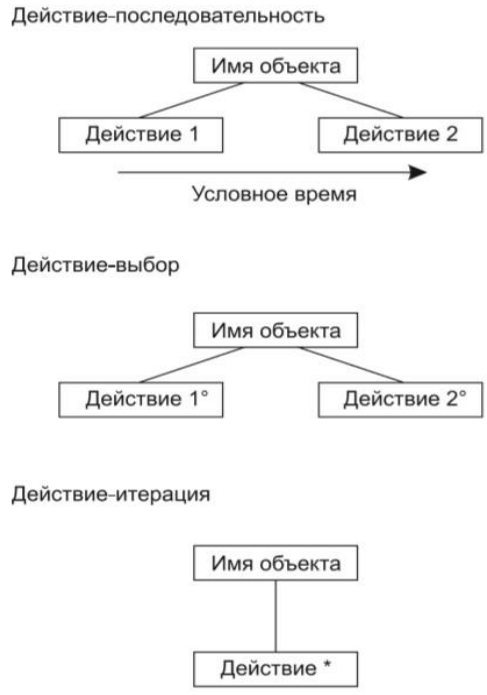
\includegraphics[width=0.3\linewidth]{images/img48.png}
    $$
    \textbf{Сервисные функции} в методе Джексона делятся на три типа:
    \begin{itemize}
        \item Встроенные функции (задаются командами в структурном тексте);
        \item Функции впечатления (наблюдают вектор состояния и вырабатывают выходные результаты);
        \item Функции диалога (наблюдают вектор состояния, формируют данные и выполняют операции).
    \end{itemize}
    \textbf{Объектный подход} к разработке сложных программных систем применяется на всех основных стадиях жизненного цикла ПО и включает:
    \begin{itemize}
        \item \textbf{OOA (object oriented analysis)} -- объектно-ориентированный анализ -- методология анализа предметной области, при которой требования к проектируемой системе воспринимаются с точки зрения классов и объектов, выявленных в предметной области;
        \item \textbf{OOD (object oriented design)} -- объектно-ориентированное проектирование -- методология проектирования, соединяющая в себе процесс объектной декомпозиции и приемы представления логической и физической, а также статической и динамической моделей проектируемой системы;
        \item \textbf{OOP (object oriented programming)} -- объектно-ориентированное программирование -- методология программирования, основанная на представлении программы в виде совокупности объектов, каждый из которых является экземпляром определенного класса, а классы образуют иерархию наследования.
    \end{itemize}
    \textbf{Базовые принципы ООАП:}
    \begin{itemize}
        \item \textbf{Декомпозиция} - разбиение целого на составные элементы;
        \item \textbf{Абстрагирование} - выделение основных элементов предметной области с одинаковой структурой и поведением;
        \item \textbf{Иерархичность};
        \item \textbf{Многомодельность}.
    \end{itemize}
    \textbf{Преимущества применения ООАП:}
    \begin{itemize}
        \item Удовлетворение требованиям заказчика;
        \item Удобство для коллективной разработки, отладки и тестирования;
        \item Прозрачность;
        \item Развиваемость;
        \item Возможность повторного использования компонентов.
    \end{itemize}
    \textbf{Процесс ООАП} можно рассматривать как последовательный переход от разработки наиболее общих моделей концептуального уровня к более детальным представлениям логического и физического уровня. В процессе ООАП на двух уровнях иерархии (концептуальном и физическом) используются статические и динамические представления сложной системы.
    $$
        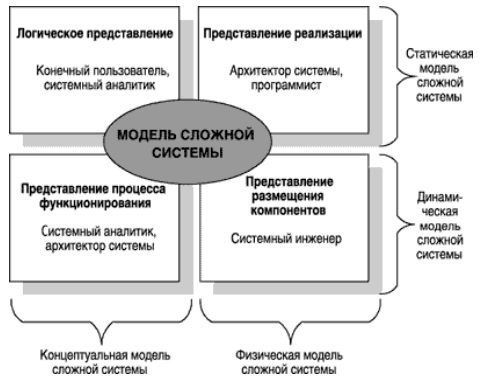
\includegraphics[width=0.5\linewidth]{images/img49.png}
    $$
    \\\\
    При объектно-ориентированном моделировании структуры системы описываются составные части системы и отношения между ними. UML является объектно-ориентированным языком моделирования, где основным видом составных частей, из которых состоит система, являются объекты.
    \\\\
    \textbf{Парадигма программирования} -- собрание основополагающих принципов, служащих методической основой конкретных технологий и инструментальных средств программирования. Центральной идеей объектно-ориентированной парадигмы является \textbf{инкапсуляция} -- структурирование программы на структуры, объединяющие данные и процедуры их обработки. 
    \\\\
    \textbf{Пользовательский интерфейс (UI)} -- внешний вид продукта, способ общения между пользователем и программой.
    \\\\
    \textbf{Графический интерфейс пользователя (GUI)} -- система средств для взаимодействия пользователя с компьютером, основанная на представлении всех доступных пользователю системных объектов и функций в виде графических компонентов экрана (окон, значков, меню, кнопок, списков и т.п.). 
    \\\\
    \textbf{Типы пользовательского интерфейса:}
    \begin{itemize}
        \item Текстовые
        \item Тактильные
        \item Голосовые
        \item Жестовые
        \item Нейронные
        \item Графические
    \end{itemize}
    \textbf{Шесть принципов проектирования пользовательского интерфейса:}
    \begin{enumerate}
        \item Структурная организация
        \item Простота
        \item Видимость
        \item Обратная связь
        \item Толерантность
        \item Повторное использование
    \end{enumerate}
\textbf{Предметно-ориентированное проектирование (Domain-Driven Design, DDD)} -- набор принципов и схем, направленных на создание оптимальных систем объектов. DDD сводится к созданию программных абстракций, которые называются \textbf{моделями предметных областей}. В эти модели входит бизнес-логика, устанавливающая связь между реальными условиями области применения продукта и кодом.
\\\\
DDD не является конкретной технологией или методологией, а представляет собой набор правил, которые позволяют принимать правильные проектные решения. Данный подход позволяет значительно ускорить процесс проектирования программного обеспечения в незнакомой предметной области.

\chapter{Компьютерные системы}
\section{Процессы и потоки}
\textbf{Процесс} — это экземпляр выполняемой программы, включающий текущие значения счётчика команд, регистров и переменных. Каждый процесс имеет своё адресное пространство — список адресов ячеек памяти, откуда процесс может считывать данные и куда может записывать их. 
\\\\
\textbf{Поток (thread)} — это набор инструкций, который будет исполняться процессором во время работы программы. У каждого потока есть свой счётчик команд, регистры для сохранения рабочих переменных и собственный стек. Потоки внутри одного процесса используют общее адресное пространство и могут совместно работать с общими данными.
\\\\
Поток может находиться \textbf{в одном из следующих состояний}:
\begin{itemize}
    \item \textbf{Выполняемый (Running)} — поток занимает центральный процессор и активно исполняется.
    \item \textbf{Готовый (Ready)} — поток готов к выполнению, но ожидает своей очереди на процессор.
    \item \textbf{Блокированный (Blocked)} — поток ожидает наступления события, например завершения операции ввода-вывода.
    \item \textbf{Завершённый (Terminated)} — поток завершил выполнение.
    \item \textbf{Подвешенный (Suspended)} — поток был приостановлен операцией \texttt{Suspend}.
\end{itemize}
$$
    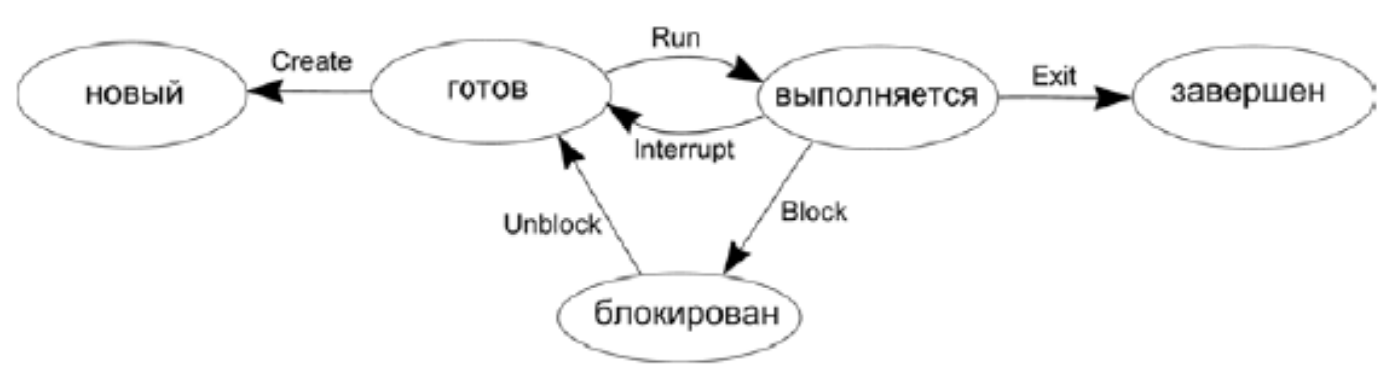
\includegraphics[width=0.5\linewidth]{images/img50.png}
$$
\textbf{Диаграмма состояний потока} включает переходы между различными состояниями:
\begin{itemize}
    \item Операция \texttt{Run} переводит поток из состояния \textit{готов} в состояние \textit{выполняется}.
    \item Операция \texttt{Interrupt} переводит поток из состояния \textit{выполняется} в состояние \textit{готов}.
    \item Операция \texttt{Block} переводит поток из состояния \textit{выполняется} в состояние \textit{блокирован}.
    \item Операция \texttt{Unblock} переводит поток из состояния \textit{блокирован} в состояние \textit{готов}.
    \item Операции \texttt{Suspend} и \texttt{Resume} позволяют приостановить и возобновить выполнение потока из любого состояния.
\end{itemize}
$$
    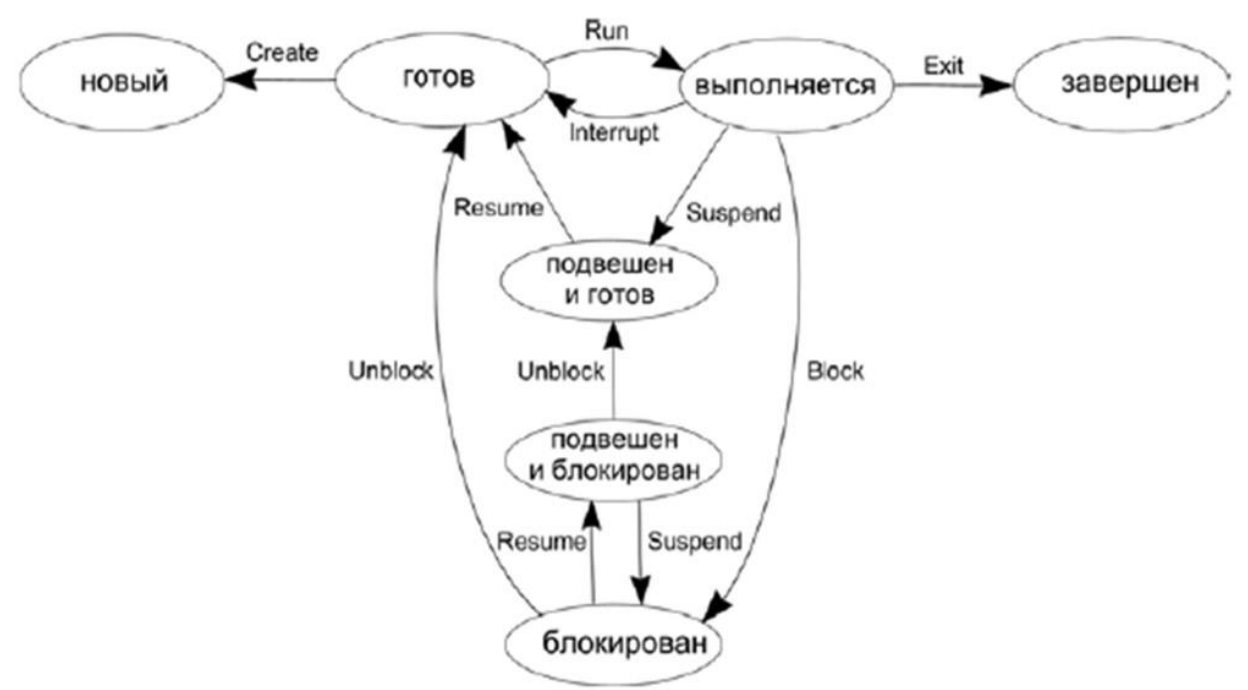
\includegraphics[width=0.5\linewidth]{images/img51.png}
$$
\textbf{Планирование процессов} — это выбор следующего процесса или потока для выполнения. В многозадачных системах одновременно может находиться в состоянии готовности несколько процессов или потоков. Планировщик решает, какой из них будет выполняться следующим, используя алгоритмы планирования. Основные цели планирования:
\begin{itemize}
    \item \textbf{Равнодоступность} — обеспечение справедливого распределения процессорного времени между процессами.
    \item \textbf{Производительность} — выполнение максимального количества заданий за единицу времени.
    \item \textbf{Баланс} — поддержание загруженности всех частей системы.
\end{itemize}
\subsection*{Алгоритмы планирования процессов}
\subsubsection*{FCFS (First Come, First Served)}
Алгоритм \textit{первым пришёл — первым обслужен} (FIFO):
\begin{itemize}
    \item Процессы выстраиваются в очередь в порядке поступления.
    \item Процесс, поступивший первым, выполняется до завершения, после чего выбирается следующий.
    \item Преимущества: простота реализации.
    \item Недостатки: возможны значительные задержки для коротких процессов из-за более длинных процессов.
\end{itemize}

\subsubsection*{SPN (Shortest Process Next)}
Алгоритм \textit{самый короткий процесс следующим}:
\begin{itemize}
    \item Выбирается процесс с наименьшим временем выполнения.
    \item Для оценки времени выполнения можно использовать данные о предыдущих выполнениях.
    \item Преимущества: минимизация среднего времени ожидания.
    \item Недостатки: длинные процессы могут голодать, так как всегда уступают место коротким.
\end{itemize}

\subsubsection*{RR (Round Robin)}
Алгоритм \textit{карусельного планирования}:
\begin{itemize}
    \item Каждому процессу назначается фиксированный квант времени.
    \item Если процесс не завершился за выделенный квант, он переводится в конец очереди.
    \item Преимущества: равномерное распределение процессорного времени.
    \item Недостатки: слишком короткий квант времени может привести к частым переключениям и снижению производительности, слишком длинный — ухудшить отклик системы.
\end{itemize}

\subsubsection*{SRT (Shortest Remaining Time)}
Алгоритм \textit{наименьшего оставшегося времени}:
\begin{itemize}
    \item Выбирается процесс с наименьшим оставшимся временем до завершения.
    \item Если новый процесс с меньшим оставшимся временем поступает в очередь, текущий процесс вытесняется.
    \item Преимущества: минимизация времени завершения.
    \item Недостатки: высокие накладные расходы на вычисление оставшегося времени, возможное голодание длинных процессов.
\end{itemize}

\section{Взаимодействие процессов}
\textbf{Синхронизация потоков} — это процесс координации выполнения потоков для достижения корректного управления общими ресурсами. Основные виды синхронизации:
\begin{itemize}
    \item \textbf{Условная синхронизация} — выполнение потока зависит от выполнения определённого условия.
    \item \textbf{Взаимное исключение} — предотвращение одновременного доступа нескольких потоков к критической секции.
\end{itemize}
\textbf{Условная синхронизация} позволяет потоку выполнять действия только при выполнении определённого условия. 
\begin{itemize}
    \item Оператор условной синхронизации: \texttt{await(условие) действие}
    \item Пример выполнения:
    \begin{enumerate}
        \item Поток ожидает выполнения условия (\texttt{await} блокирует выполнение, пока условие не станет истинным).
        \item После выполнения условия действие выполняется атомарно.
    \end{enumerate}
\end{itemize}

Пример реализации условной синхронизации:
\begin{verbatim}
bool event = false; // событие
void thread_1() {
    actions_before_event(); 
    while(!event); // ожидание события
    actions_after_event();
}
void thread_2() {
    some_actions(); 
    event = true; // оповещение о событии
    other_actions();
}
\end{verbatim}
\textbf{Взаимное исключение} — это механизм, который гарантирует, что несколько потоков не будут одновременно находиться в своих критических секциях. 
\begin{itemize}
    \item Код, выполняемый внутри критической секции, называется \textbf{критической секцией}.
    \item Основные условия для реализации взаимного исключения:
    \begin{enumerate}
        \item Два потока не могут одновременно находиться в критических секциях.
        \item Никакие предположения о скорости или количестве процессоров не должны влиять на выполнение.
        \item Потоки, находящиеся вне критических секций, не могут блокироваться.
        \item Потоки не должны находиться в вечном ожидании входа в критическую секцию.
    \end{enumerate}
\end{itemize}
\textbf{Каналы передачи данных} используются для обмена информацией между потоками, особенно если они принадлежат разным процессам. Канал — это объект операционной системы, представляющий собой область памяти, разделяемую несколькими процессами.
\\\\
\textbf{Канал обычно реализуется} как кольцевой буфер, работающий по принципу \textbf{FIFO (First In — First Out)}. 
\begin{itemize}
    \item Данные, записанные одним процессом в канал, читаются другим процессом в порядке записи.
    \item Передача данных может быть организована:
    \begin{itemize}
        \item \textbf{Потоком} — непрерывная последовательность байтов.
        \item \textbf{Сообщениями} — данные передаются группами байтов, называемыми сообщениями.
    \end{itemize}
\end{itemize}
Порядок работы канала передачи данных:
\begin{enumerate}
    \item Поток-отправитель записывает данные в буфер.
    \item Поток ядра операционной системы перемещает данные из буфера в общую память.
    \item Поток ядра перемещает данные из общей памяти в буфер потока-получателя.
    \item Поток-получатель читает данные из буфера.
\end{enumerate}
\textbf{Передача сообщений} — это механизм обмена данными между процессами через сообщения. Сообщение состоит из двух частей:
\begin{itemize}
    \item \textbf{Заголовок} — содержит тип сообщения, идентификаторы отправителя и получателя, длину сообщения и управляющую информацию.
    \item \textbf{Тело} — содержит данные сообщения.
\end{itemize}
Передача сообщений может происходить с использованием прямой или косвенной адресации:
\begin{itemize}
    \item \textbf{Прямая адресация:} процессы отправитель и получатель явно указываются в функциях \texttt{send} и \texttt{receive}.
    \begin{verbatim}
    send(P, сообщение); // отправка сообщения процессу P
    receive(Q, сообщение); // получение сообщения от процесса Q
    \end{verbatim}
    \item \textbf{Косвенная адресация:} вместо идентификаторов процессов указывается имя канала передачи данных.
    \begin{verbatim}
    send(S, сообщение); // отправка сообщения по каналу S
    receive(R, сообщение); // получение сообщения из канала R
    \end{verbatim}
\end{itemize}
Адресация может быть:
\begin{itemize}
    \item \textbf{Симметричная:} используется только один тип адресации (прямая или косвенная).
    \item \textbf{Асимметричная:} используется комбинация прямой и косвенной адресации.
\end{itemize}
Обмен данными между процессами может быть \textbf{синхронным} или \textbf{асинхронным}:
\begin{itemize}
    \item \textbf{Синхронный обмен:} 
    \begin{itemize}
        \item Поток-отправитель блокируется после вызова \texttt{send}, пока сообщение не будет получено.
        \item Поток-получатель блокируется после вызова \texttt{receive}, пока данные не будут доставлены.
    \end{itemize}
    \item \textbf{Асинхронный обмен:} 
    \begin{itemize}
        \item Поток-отправитель сразу продолжает выполнение после вызова \texttt{send}, не дожидаясь получения сообщения.
        \item Поток-получатель также не блокируется, если сообщение отсутствует.
    \end{itemize}
\end{itemize}
Синхронный обмен более надёжен, так как обеспечивает строгую координацию между потоками, но асинхронный обмен более эффективен за счёт параллельного выполнения процессов.

\section{Определение понятий <<базы данных>> и <<СУБД>>}
\textbf{СУБД} -- совокупность языковых и программных средств, предназначенных для создания, ведения и использования информации, хранящейся в БД.
\\\\
\textbf{Модель данных} -- некоторая абстракция, которая, будучи приложима к
конкретным данным, позволяет пользователям и разработчикам
трактовать их уже как информацию, т. е. как сведения, содержащие не
только данные, но и взаимосвязи между ними.
\\\\
Системы управления базами данных (СУБД) \textbf{классифицируются} по типу моделей данных, которые они поддерживают. Основные типы моделей:
\begin{itemize}
	\item \textbf{Иерархическая модель}
	\begin{itemize}
		\item \textbf{Структура:} Данные организованы в виде \textit{древовидной структуры}, где каждый элемент (узел) имеет только одного родителя, но может иметь множество потомков. Когда запись удаляется из
		дерева, все ее потомки также должны быть удалены.
		\item \textbf{Пример:} IBM IMS.
	\end{itemize}
	\item \textbf{Сетевая модель}
	\begin{itemize}
		\item \textbf{Структура:} Расширяет иерархическую модель. Позволяет одному элементу быть связанным с \textit{несколькими родителями}, поддерживаются сложные связи типа \textit{<<многие ко многим>>}.
		\item \textbf{Пример:} Integrated Data Store (IDS).
	\end{itemize}
	
	\item \textbf{Реляционная модель}
	\begin{itemize}
		\item \textbf{Структура:} Данные организованы в таблицы (отношения), строки которых --- записи, а столбцы --- поля. Каждая запись таблицы имеет одинаковую структуру. 
		\item \textbf{Преимущества:} Простота, мощный язык запросов SQL, независимость данных, хорошо приспособлены для работы в
		архитектуре клиент-сервер, позволяют параллельную обработку БД.
		\item \textbf{Примеры:} Oracle, MySQL, PostgreSQL, Microsoft SQL Server.
	\end{itemize}
	
	\item \textbf{Объектно-ориентированная модель}
	\begin{itemize}
		\item \textbf{Структура:} Данные представлены в виде объектов, поддерживаются наследование, инкапсуляция и полиморфизм.
		\item \textbf{Пример:} ObjectDB, db4o.
	\end{itemize}
	
	\item \textbf{Документо-ориентированная (NoSQL) модель}
	\begin{itemize}
		\item \textbf{Структура:} Данные хранятся в виде документов (обычно в формате JSON/BSON), что удобно для хранения неструктурированных или слабо структурированных данных.
		\item \textbf{Пример:} MongoDB, CouchDB.
	\end{itemize}
	
	\item \textbf{Ключ-значение, графовые и другие модели}
	\begin{itemize}
		\item \textbf{Ключ-значение:} Простая структура, где каждому ключу соответствует определённое значение (Redis, Riak).
		\item \textbf{Графовые:} Данные представлены в виде графов --- узлы и рёбра (Neo4j, ArangoDB).
	\end{itemize}
\end{itemize}
\textbf{Настольные локальные СУБД:}
\begin{itemize}
	\item \textbf{Архитектура:} СУБД и данные находятся на одном компьютере, обычно используются одним пользователем или малой группой.
	\item \textbf{Преимущества:} Простота установки, низкие требования к ресурсам, удобство для небольших проектов или персонального использования.
	\item \textbf{Ограничения:} Ограниченная масштабируемость, низкая производительность при большом количестве пользователей, слабая защита данных.
	\item \textbf{Примеры:} Microsoft Access, SQLite, dBASE, Paradox.
\end{itemize}
\textbf{Клиент-серверные СУБД:}
\begin{itemize}
	\item \textbf{Архитектура:} СУБД работает на сервере, а пользователи подключаются к ней через сеть с помощью клиентских приложений. Центральная машина (сервер базы данных) помимо хранения базы данных обеспечивает выполнение основного объема обработки данных. Запрос клиента (рабочей станции) порождает поиск и извлечение данных на сервере, которые затем транспортируются по сети к клиенту.
	\item \textbf{Преимущества:} Высокая производительность, централизованное управление, возможность работы с большим количеством пользователей, масштабируемость, безопасность.
	\item \textbf{Ограничения:} Большие вычислительные ресурсы, потребляемые
	сервером.
	\item \textbf{Примеры:} Oracle, Microsoft SQL Server, PostgreSQL, MySQL.
\end{itemize}
\textbf{Схема работы:}
\begin{center}
	Клиент $\longleftrightarrow$ Сеть $\longleftrightarrow$ Сервер СУБД $\longleftrightarrow$ Хранилище данных
\end{center}
Главной составляющей в \textbf{жизненном цикле БД} является создание единой базы данных и программ, необходимых для ее работы. Жизненный цикл БД включает в себя следующие основные этапы:
$$
	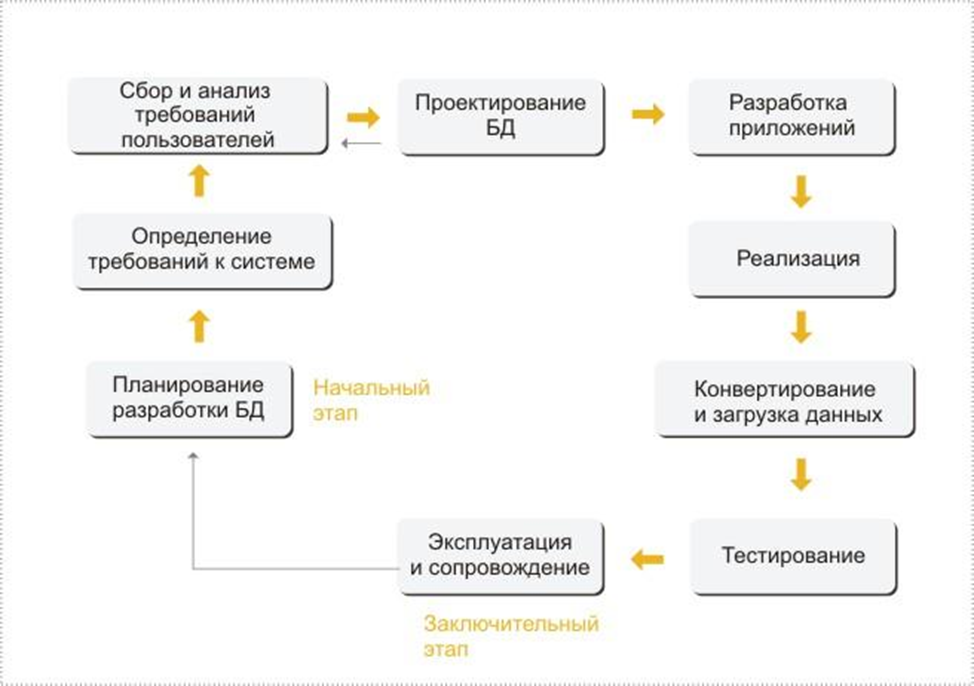
\includegraphics[scale=0.5]{images/img52}
$$
Полный цикл разработки базы данных включает \textbf{концептуальное}, \textbf{логическое} и \textbf{физическое} ее проектирование.
\begin{enumerate}
	\item \textbf{Концептуальное проектирование базы данных}.
	Цель этого концептуального проектирования -- создание концептуальной модели данных исходя из представлений пользователей о предметной области.
	В построении общей концептуальной модели данных выделяют ряд этапов.
	\begin{itemize}
		\item Выделение локальных представлений, соответствующих обычно относительно независимым данным. Каждое такое представление проектируется как подзадача.
		\item Формулирование сущностей, описывающих локальную предметную область проектируемой БД, и описание атрибутов, составляющих структуру каждой сущности.
		\item Выделение ключевых атрибутов.
		\item Спецификация связей между сущностями. Удаление избыточных связей.
		\item Анализ и добавление неключевых атрибутов.
		\item Объединение локальных представлений.
	\end{itemize}
	\item \textbf{Логическое проектирование базы данных}.
	Цель этапа логического проектирования -- преобразование концептуальной модели на основе выбранной модели данных в логическую модель, не зависимую от особенностей используемой в дальнейшем СУБД для физической реализации базы данных.
	\item \textbf{Физическое проектирование базы данных}.
	Цель этапа физического проектирования -- описание конкретной реализации базы данных, размещаемой во внешней памяти компьютера.
\end{enumerate}

\section{Проектирование баз данных. Реляционная модель базы данных. Нормализация данных, типы нормальных форм}
\textbf{Проектирование базы данных (БД)} --- это процесс создания структуры хранения и организации данных, который обеспечивает эффективное хранение, обработку и извлечение информации. Основные этапы проектирования БД:
\begin{itemize}
	\item \textbf{Сбор требований:} Определение целей БД, анализ предметной области и информации, которую необходимо хранить.
	\item \textbf{Концептуальное проектирование:} Описание данных на высоком уровне абстракции с помощью схем (например, ER-диаграмм).
	\item \textbf{Логическое проектирование:} Преобразование концептуальной модели в логическую, обычно в реляционную модель (таблицы, поля, связи).
	\item \textbf{Физическое проектирование:} Определение методов хранения данных, индексов, оптимизация запросов и структуры хранения.
\end{itemize}
\textbf{Реляционная модель} --- это наиболее распространённая логическая модель данных, в которой информация хранится в виде таблиц (отношений).
\begin{itemize}
	\item \textbf{Таблица (отношение):} Множество строк (кортежей) и столбцов (атрибутов).
	\item \textbf{Кортеж:} Строка таблицы, представляющая отдельную запись.
	\item \textbf{Атрибут:} Столбец таблицы, представляющий отдельное свойство.
	\item \textbf{Домен:} Множество допустимых значений для атрибута.
\end{itemize}
Преимущества реляционной модели: простота структуры, гибкость и мощные возможности для запросов (язык SQL).
\\\\
\textbf{Ключ} --- минимальный набор атрибутов, однозначно идентифицирующий каждую запись в таблице.
\begin{itemize}
	\item \textbf{Первичный ключ (Primary Key):} Уникальный идентификатор каждой строки таблицы.
	\item \textbf{Кандидатный ключ (Candidate Key):} Любой минимальный набор атрибутов, способный быть первичным ключом.
	\item \textbf{Альтернативный ключ (Alternate Key):} Кандидатный ключ, не выбранный в качестве первичного.
	\item \textbf{Внешний ключ (Foreign Key):} Атрибут, ссылающийся на первичный ключ другой таблицы для организации связей между таблицами.
\end{itemize}
\textbf{Требования к ключам:}
\begin{itemize}
	\item Уникальность: значения ключа не повторяются.
	\item Минимальность: нет лишних атрибутов.
	\item Неизменяемость: значения ключа не должны меняться.
	\item Не допускаются пустые значения (NULL) в первичном ключе.
\end{itemize}
$$
	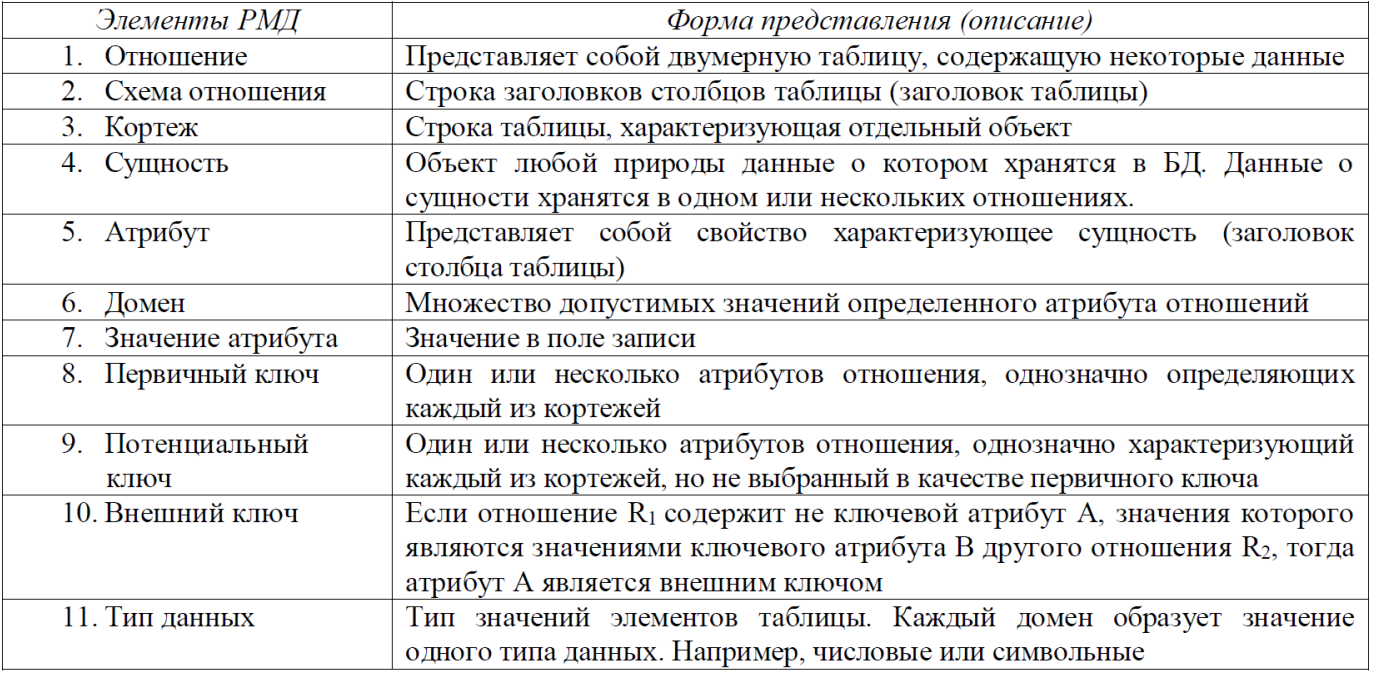
\includegraphics[scale=0.5]{images/img54}
$$
\textbf{Функциональная зависимость} --- отношение между двумя наборами атрибутов, при котором значению одного набора однозначно соответствует значение другого.
Обозначается: $A \rightarrow B$, что означает: \textit{атрибут $B$ функционально зависит от атрибута $A$}.
\begin{itemize}
	\item \textbf{Полная функциональная зависимость:} Атрибут $B$ зависит от всего набора атрибутов $A$.
	\item \textbf{Частичная зависимость:} Атрибут $B$ зависит только от части составного ключа.
	\item \textbf{Транзитивная зависимость:} Атрибут $C$ зависит от $B$, а $B$ зависит от $A$.
\end{itemize}
\textbf{Нормализация} --- это процесс организации структуры данных в реляционной базе с целью устранения избыточности и обеспечения целостности данных. Она проводится путём разбиения таблиц и установления между ними связей.
\\\\
\textbf{Цели нормализации:}
\begin{itemize}
	\item Уменьшение избыточности данных
	\item Устранение аномалий обновления, вставки и удаления
	\item Обеспечение целостности данных
\end{itemize}
\textbf{Нормальные формы} --- это стандартизированные требования к структуре таблиц, направленные на устранение различных видов избыточности и аномалий.
\begin{itemize}
	\item \textbf{Первая нормальная форма (1NF):} Все атрибуты содержат только атомарные (неделимые) значения, нет повторяющихся групп.
	\item \textbf{Вторая нормальная форма (2NF):} Таблица находится в 1NF и каждый неключевой атрибут полностью функционально зависит от первичного ключа.
	\item \textbf{Третья нормальная форма (3NF):} Таблица находится во 2NF и не содержит транзитивных зависимостей между неключевыми атрибутами.
	\item \textbf{Нормальная форма Бойса-Кодда (BCNF):} Более строгая версия 3NF: для всякой нетривиальной функциональной зависимости левый атрибут --- суперключ.
	\item \textbf{Четвёртая нормальная форма (4NF):} Устраняет многозначные зависимости; таблица находится в BCNF и не содержит неминимальных многозначных зависимостей.
	\item \textbf{Пятая нормальная форма (5NF):} Устраняет соединительные зависимости; таблица находится в 4NF и каждая соединительная зависимость является следствием кандидата ключа.
\end{itemize}
$$
	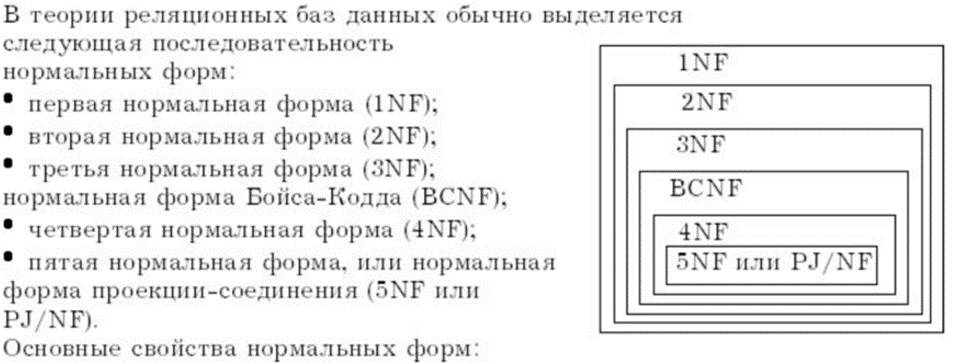
\includegraphics[scale=0.5]{images/img53}
$$
Рассмотрим таблицу, не находящуюся в нормальных формах:
\begin{center}
	\begin{tabular}{|l|l|l|}
		\hline
		\textbf{Студент} & \textbf{Курс} & \textbf{Преподаватель} \\
		\hline
		Иванов & Математика, Физика & Иванова, Петров \\
		\hline
		Петров & Химия & Сидоров \\
		\hline
	\end{tabular}
\end{center}
\begin{itemize}
	\item Для 1NF разделим значения на атомарные:
	\begin{center}
		\begin{tabular}{|l|l|l|}
			\hline
			\textbf{Студент} & \textbf{Курс} & \textbf{Преподаватель} \\
			\hline
			Иванов & Математика & Иванова \\
			Иванов & Физика & Петров \\
			Петров & Химия & Сидоров \\
			\hline
		\end{tabular}
	\end{center}
	\item На следующих шагах нормализации таблица может быть разделена на две:
	\begin{itemize}
		\item <<Студент-Курс>>
		\item <<Курс-Преподаватель>>
	\end{itemize}
\end{itemize}

\section{Язык SQL}
\textbf{SQL (Structured Query Language)} --- это стандартный язык программирования для работы с реляционными базами данных. Он предназначен для определения, изменения, извлечения и управления данными.
\\\\
Язык SQL делится на несколько подсистем:
\begin{itemize}
	\item \textbf{Язык определения данных (DDL --- Data Definition Language)}
	\item \textbf{Язык манипулирования данными (DML --- Data Manipulation Language)}
	\item \textbf{Язык управления транзакциями (TCL --- Transaction Control Language)}
	\item \textbf{Язык управления доступом (DCL --- Data Control Language)}
\end{itemize}
\subsubsection*{Язык определения данных (DDL)}
\textbf{DDL} предназначен для создания, изменения и удаления объектов базы данных (таблиц, индексов, представлений и т.д.).
\\\\
Основные операторы DDL:
\begin{itemize}
	\item \texttt{CREATE} --- создание новых объектов (например, \texttt{CREATE TABLE})
	\item \texttt{ALTER} --- изменение структуры существующих объектов (например, добавление столбцов)
	\item \texttt{DROP} --- удаление объектов
	\item \texttt{TRUNCATE} --- удаление всех данных из таблицы с сохранением структуры
\end{itemize}
\textbf{Пример создания таблицы:}
\begin{verbatim}
	CREATE TABLE Students (
	StudentID INT PRIMARY KEY,
	Name VARCHAR(50),
	Age INT
	);
\end{verbatim}
\subsubsection*{Язык манипулирования данными (DML)}
\textbf{DML} используется для работы с данными внутри таблиц: добавление, изменение, удаление и выборка данных.
\\\\
Основные операторы DML:
\begin{itemize}
	\item \texttt{SELECT} --- выборка данных
	\item \texttt{INSERT} --- добавление новых строк
	\item \texttt{UPDATE} --- изменение существующих строк
	\item \texttt{DELETE} --- удаление строк
\end{itemize}
\textbf{Примеры:}
\begin{verbatim}
	-- Добавление данных
	INSERT INTO Students (StudentID, Name, Age) VALUES (1, 'Иванов', 19);
	
	-- Изменение данных
	UPDATE Students SET Age = 20 WHERE StudentID = 1;
	
	-- Удаление данных
	DELETE FROM Students WHERE StudentID = 1;
	
	-- Выборка данных
	SELECT * FROM Students WHERE Age > 18;
\end{verbatim}
\subsection*{Транзакции и управление транзакциями}
\textbf{Транзакция} --- это последовательность операций с базой данных, которая либо выполняется полностью, либо не выполняется вовсе, обеспечивая целостность данных.
\\\\
Основные свойства транзакций (ACID):
\begin{itemize}
	\item \textbf{Atomicity (атомарность):} Все операции транзакции выполняются как единое целое.
	\item \textbf{Consistency (согласованность):} После выполнения транзакции данные отвечают всем правилам целостности.
	\item \textbf{Isolation (изоляция):} Одновременное выполнение транзакций не влияет друг на друга.
	\item \textbf{Durability (устойчивость):} После завершения транзакции изменения сохраняются даже при сбоях.
\end{itemize}
SQL предоставляет специальные \textbf{операторы для управления транзакциями}:
\begin{itemize}
	\item \texttt{BEGIN TRANSACTION} или \texttt{START TRANSACTION} --- начало транзакции
	\item \texttt{COMMIT} --- фиксация изменений, внесённых транзакцией
	\item \texttt{ROLLBACK} --- отмена изменений, внесённых транзакцией
	\item \texttt{SAVEPOINT} --- создание промежуточной точки сохранения внутри транзакции
	\item \texttt{RELEASE SAVEPOINT} --- удаление точки сохранения
\end{itemize}
\textbf{Пример работы с транзакциями:}
\begin{verbatim}
	START TRANSACTION;
	UPDATE Students SET Age = 21 WHERE StudentID = 2;
	DELETE FROM Students WHERE StudentID = 3;
	COMMIT;
\end{verbatim}
Если при выполнении операций возникает ошибка, можно отменить все изменения так:
\begin{verbatim}
	ROLLBACK;
\end{verbatim}
\chapter{Компьютерные сети}
\section{Основные понятия компьютерных сетей. Принципы организации. Сетевые протоколы}
\textbf{Компьютерная сеть} --- это совокупность:
\begin{itemize}
	\item каналов связи;
	\item устройств приема и передачи данных;
	\item коммуникационного оборудования и сетевого программного обеспечения для объединения компьютеров и обеспечения передачи данных между ними.
\end{itemize}
Компьютерные сети \textbf{создаются для}:
\begin{itemize}
	\item Обеспечения совместного использования ресурсов (файлов, принтеров, соединения с интернетом)
	\item Повышения эффективности обмена информацией между пользователями
	\item Централизованного управления, резервного копирования и безопасности данных
	\item Удалённого доступа к программам и ресурсам
	\item Организации коллективной работы
\end{itemize}
\textbf{Интерфейс} --- совокупность аппаратных и программных средств, обеспечивающих взаимодействие между компонентами сети (например, между компьютером и сетевым оборудованием).
\\\\
\textbf{Проблемы связи нескольких компьютеров:}
\begin{itemize}
	\item \textbf{Выбор физической топологии:} Определяет, как компьютеры физически соединены между собой (шина, звезда, кольцо, ячеистая и др.)
	
	\item \textbf{Адресация узлов:} Необходимо уникально идентифицировать каждый узел сети (например, с помощью MAC-адресов, IP-адресов)
	\item \textbf{Коммутация:}
	\begin{itemize}
		\item \textit{Определение потоков:} Разделение трафика по направлениям
		\item \textit{Определение маршрутов:} Выбор оптимального пути передачи данных
		\item \textit{Коммутация в транзитном узле:} Перенаправление пакетов через промежуточные устройства (например, маршрутизаторы, коммутаторы)
		\item \textit{Мультиплексирование и демультиплексирование:} Совместная передача нескольких потоков данных по одному физическому каналу и их последующее разделение
	\end{itemize}
\end{itemize}
Компьютерные сети \textbf{классифицируются} по различным критериям:
\begin{itemize}
	\item \textbf{По масштабу:}
	\begin{itemize}
		\item \textbf{LAN (Local Area Network):} Локальная сеть (например, сеть в офисе)
		\item \textbf{MAN (Metropolitan Area Network):} Городская сеть
		\item \textbf{WAN (Wide Area Network):} Глобальная сеть (например, Интернет)
	\end{itemize}
	\item \textbf{По способу управления:}
	\begin{itemize}
		\item \textbf{Сети с выделенным сервером}
		\item \textbf{Одноранговые (peer-to-peer) сети}
	\end{itemize}
	\item \textbf{По топологии:} Шина, звезда, кольцо, дерево, сетка и др.
	$$
		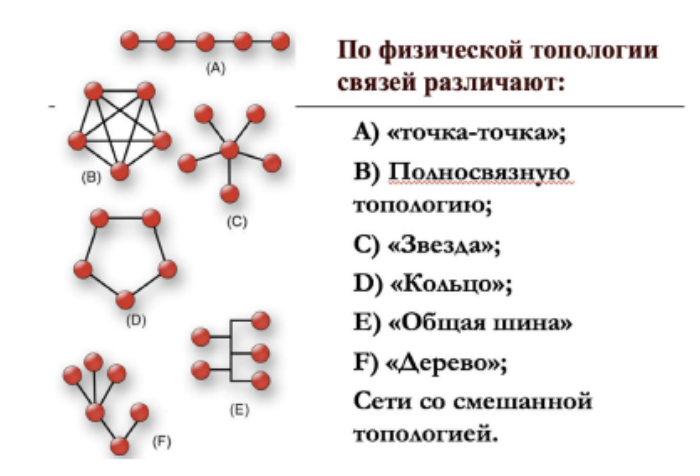
\includegraphics[scale=0.5]{images/img55}
	$$
\end{itemize}
\textbf{Протокол} --- формализованный набор правил и соглашений, определяющих формат, порядок передачи, обработку и интерпретацию данных между устройствами сети.
\\\\
\textbf{Межуровневый интерфейс} --- стандартизированное взаимодействие между уровнями архитектуры сети, позволяющее реализовывать независимость между уровнями.
\\\\
\textbf{Стек протоколов} --- иерархически организованный набор протоколов, где каждый уровень отвечает за определённую функцию при передаче данных.
\\\\
\textbf{Модель OSI (Open Systems Interconnection Reference Model)} состоит из 7 уровней:
\begin{enumerate}
	\item Прикладной (Application)
	\item Представительный (Presentation)
	\item Сеансовый (Session)
	\item Транспортный (Transport)
	\item Сетевой (Network)
	\item Канальный (Data Link)
	\item Физический (Physical)
\end{enumerate}
Каждый уровень выполняет определённые задачи и взаимодействует с соседними уровнями через чётко определённые интерфейсы.
\\\\
\textbf{Модель TCP/IP}, лежащая в основе современных сетей (включая Интернет), включает 4 уровня:
\begin{enumerate}
	\item Прикладной (Application)
	\item Транспортный (Transport)
	\item Сетевой (Internet)
	\item Сетевой доступ (Network Access, Link)
\end{enumerate}
\textbf{Сопоставление моделей:}
\begin{figure}[h!]
	\centering
	\begin{tikzpicture}[node distance=0.5cm, font=\small]
		% OSI Levels
		\node[draw,minimum width=2.5cm,minimum height=0.7cm,fill=blue!10] (osi7) {7. Прикладной};
		\node[draw,minimum width=2.5cm,minimum height=0.7cm,fill=blue!10,below=of osi7] (osi6) {6. Представительный};
		\node[draw,minimum width=2.5cm,minimum height=0.7cm,fill=blue!10,below=of osi6] (osi5) {5. Сеансовый};
		\node[draw,minimum width=2.5cm,minimum height=0.7cm,fill=blue!10,below=of osi5] (osi4) {4. Транспортный};
		\node[draw,minimum width=2.5cm,minimum height=0.7cm,fill=blue!10,below=of osi4] (osi3) {3. Сетевой};
		\node[draw,minimum width=2.5cm,minimum height=0.7cm,fill=blue!10,below=of osi3] (osi2) {2. Канальный};
		\node[draw,minimum width=2.5cm,minimum height=0.7cm,fill=blue!10,below=of osi2] (osi1) {1. Физический};
		\node[align=center, font=\bfseries, above=0.2cm of osi7] {Модель OSI};
		
		% TCP/IP Levels
		\node[draw,minimum width=2.5cm,minimum height=1.4cm,fill=green!10,right=2.2cm of osi6] (tcpip4) {Прикладной};
		\node[draw,minimum width=2.5cm,minimum height=0.7cm,fill=green!10,below=of tcpip4] (tcpip3) {Транспортный};
		\node[draw,minimum width=2.5cm,minimum height=0.7cm,fill=green!10,below=of tcpip3] (tcpip2) {Интернет};
		\node[draw,minimum width=2.5cm,minimum height=1.4cm,fill=green!10,below=of tcpip2] (tcpip1) {Сетевой доступ};
		\node[align=center, font=\bfseries, above=0.2cm of tcpip4] {Модель TCP/IP};
		
		% Линии соответствия
		\draw[->,thick] (osi7.east) -- (tcpip4.west);
		\draw[->,thick] (osi6.east) -- (tcpip4.west);
		\draw[->,thick] (osi5.east) -- (tcpip4.west);
		\draw[->,thick] (osi4.east) -- (tcpip3.west);
		\draw[->,thick] (osi3.east) -- (tcpip2.west);
		\draw[->,thick] (osi2.east) -- (tcpip1.west);
		\draw[->,thick] (osi1.east) -- (tcpip1.west);
	\end{tikzpicture}
	\caption{Сравнение уровней моделей OSI и TCP/IP}
\end{figure}
На прикладном уровне стека TCP/IP работают различные \textbf{протоколы}, отвечающие за разные виды передачи данных:
\begin{itemize}
	\item \textbf{HTTP (Hypertext Transfer Protocol):} Протокол передачи гипертекста (основа WWW)
	\item \textbf{FTP (File Transfer Protocol):} Протокол передачи файлов
	\item \textbf{SMTP (Simple Mail Transfer Protocol):} Протокол передачи электронной почты
	\item \textbf{POP3 (Post Office Protocol 3):} Протокол получения электронной почты
	\item \textbf{IMAP (Internet Message Access Protocol):} Протокол доступа к электронной почте
	\item \textbf{DNS (Domain Name System):} Протокол разрешения доменных имён
	\item \textbf{DHCP (Dynamic Host Configuration Protocol):} Протокол автоматической настройки IP-адресов
	\item \textbf{Telnet, SSH:} Протоколы удалённого доступа к командной строке
\end{itemize}


\section{Основные принципы построения и архитектура сети Интернет. Алгоритмы и протоколы внешней и внутренней маршрутизации}

Современные компьютерные сети, включая Интернет, представляют собой сложную иерархическую структуру, основанную на взаимодействии множества автономных систем (АС). Для обеспечения передачи данных между узлами сети используется маршрутизация — процесс выбора оптимального пути для передачи пакетов данных. Основы маршрутизации включают алгоритмы и протоколы, которые обеспечивают работу как внутри автономной системы, так и между ними.
\\\\
\textbf{Понятие автономной системы} подразумевает совокупность сетей, находящихся под управлением одной или нескольких организаций и использующих единую политику маршрутизации. Каждой АС присваивается \textbf{уникальный номер (ASN, {Autonomous System Number})}, который используется для идентификации в глобальной сети. Главной \textbf{целью маршрутизации} является обеспечение доставки пакетов данных от источника к получателю с минимальными затратами ресурсов и времени. \textbf{Задачи маршрутизации} включают:

\begin{itemize}
	\item \textbf{Определение оптимального маршрута} для передачи данных.
	\item \textbf{Обеспечение устойчивости сети} при изменениях в её структуре.
	\item \textbf{Минимизация задержек и потерь данных} в процессе передачи.
\end{itemize}
Для выполнения этих задач используются различные алгоритмы маршрутизации. \textbf{Основные подходы:}
\begin{itemize}
	\item \textbf{Дистанционно-векторные алгоритмы} основаны на обмене информацией о расстояниях (метриках) до сетей между соседними маршрутизаторами. Каждый маршрутизатор поддерживает таблицу маршрутизации и периодически обновляет её, обмениваясь данными с соседями. Примером такого алгоритма является алгоритм Беллмана-Форда.
	\\\\ 
	Протокол \textbf{RIP ({Routing Information Protocol})} является реализацией дистанционно-векторного подхода. Его основные характеристики:
	\begin{itemize}
		\item Использование метрики на основе количества переходов (hop count).
		\item Ограничение максимальной длины маршрута (15 прыжков).
		\item Периодическое обновление таблиц маршрутизации (каждые 30 секунд).
		\item Простота реализации, но ограниченная масштабируемость.
	\end{itemize}
	\item \textbf{Алгоритмы состояния связей (Link-State Routing Algorithms}) используют информацию о состоянии всех соединений в сети. Каждое устройство строит полную карту сети и рассчитывает оптимальный маршрут с использованием алгоритма Дейкстры. 
	\\\\
	Протокол \textbf{OSPF ({Open Shortest Path First})} является примером реализации данного подхода. Основные особенности OSPF:
	\begin{itemize}
		\item Использование метрики на основе стоимости ({cost}), которая может учитывать полосу пропускания, задержки и другие параметры.
		\item Разделение сети на области ({areas}), что повышает масштабируемость.
		\item Быстрое обновление маршрутов при изменении топологии (поддержка концепции LSA, {Link-State Advertisement}).
	\end{itemize}
	\textbf{EIGRP (Enhanced Interior Gateway Routing Protocol}) — протокол, разработанный компанией Cisco, который сочетает преимущества дистанционно-векторных алгоритмов и алгоритмов состояния связей. Он использует алгоритм DUAL ({Diffusing Update Algorithm}) для выбора оптимального маршрута и обеспечения устойчивости сети. Особенности EIGRP:
	\begin{itemize}
		\item Быстрое восстановление маршрутов при сбоях.
		\item Использование нескольких метрик (полоса пропускания, задержки, надёжность и загруженность).
		\item Поддержка как IPv4, так и IPv6.
	\end{itemize}
\end{itemize}
Для маршрутизации между автономными системами используется \textbf{протокол BGP (Border Gateway Protocol}). BGP является основным протоколом внешней маршрутизации в Интернете. Его ключевые характеристики:
\begin{itemize}
	\item Основан на политике маршрутизации, позволяющей администраторам управлять выбором маршрутов.
	\item Использует TCP для надёжной передачи данных.
	\item Передаёт информацию о доступных маршрутах и не рассчитывает оптимальные маршруты самостоятельно, предоставляя эту задачу администраторам.
	\item Поддерживает сложные политики фильтрации маршрутов и управления трафиком.
\end{itemize}
\end{document}